\documentclass[12pt,notitlepage]{aghdpl}
% \documentclass[en,11pt]{aghdpl}  % praca w języku angielskim

% Lista wszystkich języków stanowiących języki pozycji bibliograficznych użytych w pracy.
% (Zgodnie z zasadami tworzenia bibliografii każda pozycja powinna zostać utworzona zgodnie z zasadami języka, w którym dana publikacja została napisana.)
\usepackage[english,polish]{babel}

% Użyj polskiego łamania wyrazów (zamiast domyślnego angielskiego).
\usepackage{polski}

\usepackage[utf8]{inputenc}

% dodatkowe pakiety
\usepackage{mathtools}
\usepackage{amsfonts}
\usepackage{amsmath}
\usepackage{hyperref}
\usepackage{amsthm}


% --- < bibliografia > ---

\usepackage[
style=numeric,
sorting=none,
%
% Zastosuj styl wpisu bibliograficznego właściwy językowi publikacji.
language=autobib,
autolang=other,
% Zapisuj datę dostępu do strony WWW w formacie RRRR-MM-DD.
urldate=iso8601,
% Nie dodawaj numerów stron, na których występuje cytowanie.
backref=false,
% Podawaj ISBN.
isbn=true,
% Nie podawaj URL-i, o ile nie jest to konieczne.
url=true,
%
% Ustawienia związane z polskimi normami dla bibliografii.
maxbibnames=3,
% Jeżeli używamy BibTeXa:
backend=bibtex
]{biblatex}

\usepackage{csquotes}
% Ponieważ `csquotes` nie posiada polskiego stylu, można skorzystać z mocno zbliżonego stylu chorwackiego.
\DeclareQuoteAlias{croatian}{polish}

\addbibresource{praca_pliki/bibliografia.bib}
\renewcommand{\labelitemii}{$\bullet$}
\usepackage{tabto}

% Nie wyświetlaj wybranych pól.
%\AtEveryBibitem{\clearfield{note}}


% ------------------------
% --- < listingi > ---

% Użyj czcionki kroju Courier.
\usepackage{courier}

\usepackage{listings}
\lstloadlanguages{TeX}

\lstset{
	literate={ą}{{\k{a}}}1
           {ć}{{\'c}}1
           {ę}{{\k{e}}}1
           {ó}{{\'o}}1
           {ń}{{\'n}}1
           {ł}{{\l{}}}1
           {ś}{{\'s}}1
           {ź}{{\'z}}1
           {ż}{{\.z}}1
           {Ą}{{\k{A}}}1
           {Ć}{{\'C}}1
           {Ę}{{\k{E}}}1
           {Ó}{{\'O}}1
           {Ń}{{\'N}}1
           {Ł}{{\L{}}}1
           {Ś}{{\'S}}1
           {Ź}{{\'Z}}1
           {Ż}{{\.Z}}1,
	basicstyle=\footnotesize\ttfamily,
}

% ------------------------

\AtBeginDocument{
	\renewcommand{\tablename}{Tabela}
	\renewcommand{\figurename}{Rys.}
}

% ------------------------
% --- < tabele > ---
\usepackage{relsize}
\usepackage{array}
\usepackage{tabularx}
\usepackage{multirow}
\usepackage{booktabs}
\usepackage{makecell}
\usepackage[flushleft]{threeparttable}
\usepackage{graphicx}
\usepackage[table,x11names]{xcolor}
\usepackage[toc,page]{appendix}	
% defines the X column to use m (\parbox[c]) instead of p (`parbox[t]`)
\newcolumntype{C}[1]{>{\hsize=#1\hsize\centering\arraybackslash}X}

%---------------------------------------------------------------------------

\author{Miłosz Mach}
\shortauthor{M. Mach}

%\titlePL{Przygotowanie bardzo długiej i pasjonującej pracy dyplomowej w~systemie~\LaTeX}
%\titleEN{Preparation of a very long and fascinating bachelor or master thesis in \LaTeX}

\titlePL{Wbudowany system wizyjny do śledzenia obiektów dla potrzeb nawigacji bezzałogowego statku powietrznego (UAV)}
\titleEN{Embedded vision-based tracking system for unmanned aerial vehicle (UAV)}


\shorttitlePL{Wbudowany system wizyjny do śledzenia obiektów dla potrzeb nawigacji bezzałogowego statku powietrznego (UAV)} % skrócona wersja tytułu jeśli jest bardzo długi
\shorttitleEN{Embedded vision-based tracking system for unmanned aerial vehicle (UAV)}

\thesistype{Praca dyplomowa magisterska}
%\thesistype{Master of Science Thesis}

\supervisor{dr inż. Tomasz Kryjak}
%\supervisor{Tomasz Kryjak PhD}

\degreeprogramme{Automatyka i Robotyka}
%\degreeprogramme{Automatics and Robotics}

\date{2017}

\department{Katedra Automatyki i Inżynierii Biomedycznej}
%\department{Department of Applied Computer Science}

\faculty{Wydział Elektrotechniki, Automatyki,\protect\\[-1mm] Informatyki i Inżynierii Biomedycznej}
%\faculty{Faculty of Electrical Engineering, Automatics, Computer Science and Biomedical Engineering}

\acknowledgements{Serdecznie dziękuję mojemu promotorowi Panu dr inż. Tomaszowi Kryjakowi, za wsparcie merytoryczne oraz bliskim za cierpliwość w trakcie pisania tej pracy.}


\setlength{\cftsecnumwidth}{10mm}

%---------------------------------------------------------------------------
\setcounter{secnumdepth}{4}
\brokenpenalty=10000\relax

\begin{document}
\graphicspath{{praca_pliki/}}
\nocite{*}

\titlepages

% Ponowne zdefiniowanie stylu `plain`, aby usunąć numer strony z pierwszej strony spisu treści i poszczególnych rozdziałów.
\fancypagestyle{plain}
{
	% Usuń nagłówek i stopkę
	\fancyhf{}
	% Usuń linie.
	\renewcommand{\headrulewidth}{0pt}
	\renewcommand{\footrulewidth}{0pt}
}

\setcounter{tocdepth}{2}
\tableofcontents
\clearpage

\begin{abstract}

W pracy przedstawiona została sprzętowa realizacja detekcji i śledzenia osoby na potrzeby autonomizacji bezzałogowego statku powietrznego (UAV). System wizyjny stworzono przy wieloskalowym wykorzystaniu deskryptora HOG i klasyfikatora SVM, z niezależnym wsparciem algorytmu MeanShift. Zastosowanie potokowego przetwarzania obrazu pozwoliło na realizację obliczeń w czasie rzeczywistym dla sygnału wideo o rozdzielczości $1280\times 720$ i $60$ klatkach na sekundę dla algorytmu MeanShift i $30$ klatkach na sekundę dla metody HOG+SVM. Przedstawiany projekt został napisany w języku opisu sprzętu System Verilog i C++, oraz uruchomiony w układzie Zynq SoC znajdującym się na karcie uruchomieniowej PYNQ. %Nie wiem jak skategoryzować HOG+SVM, jeśli jest nie jest potokowo implementowany

Dzięki wykorzystaniu heterogenicznego układu Zynq możliwe było zrealizowanie wbudowanego systemu wizyjnego do sterowania bezzałogowym statkiem latającym, realizującym zadanie utrzymywania stałej pozycji względem wykrytej osoby. Poprawne działanie systemu zostało zweryfikowane podczas praktycznych testów.
%Projekt systemu również został opisany w tej pracy.
\end{abstract}

\selectlanguage{english} 
\begin{abstract}
This paper describes a hardware realization of human detection and tracking for unmanned aerial vehicle (UAV). The vision system -- based on a multi-scale approach -- was created using HOG descriptor and SVM classifier, with an independent support of a MeanShift algorithm. 
Hardware implementation and pipelining of image processing allowed to compute $1280\times 720$, $60$fps video signal in real time for MeanShift, and $30$fps for HOG+SVM method. The project was created in hardware description language -- System Verilog -- and C++ and was designed for Zynq SoC which is the part of a PYNQ board.

With a deployment on a heterogenous Zynq platform it was possible to create an embedded vision system, which allowed to control an unmanned aerial vehicle with an intention of following the detected person. The correct operation of this system was verified during practical tests.
 %That system has been described in this document as well.
\end{abstract}

%TODO 2 Uwagi do abstraktu. Zasadniczo OK, ale... pierwsze zdanie trzeba skrócić i doać inforamcę o tym UAV. No taka parafraza tytułu. Potem już te algorytmy. Na koniec dodać jedno zdanie, np. Dzięki wkorzystaniu heterogrnicznego układu Zynq... udało się  oraz, że zostało to zweryfikowane w praktyce. %ODP OK

\selectlanguage{polish} 
\chapter{Wstęp}
\label{cha:wstep}

Bezzałogowe statki powietrzne, potocznie nazywane dronami, zyskują w ostatnich latach coraz większe zainteresowanie. 
Według raportu portalu Business Insider z czerwca 2016 roku \cite{BInsider}, światowy rynek bezzałogowych statków powietrznych powiększy swoją wartość z niecałych 6 mld \$ w 2013 roku do prawie 13 mld \$ w roku 2024. 
Biorąc pod uwagę podstawowy podział maszyn -- ze względu na przeznaczenie -- raport ten wskazuje na rosnący trend zarówno w przypadku przemysłu obronnego, jak i cywilnego. Można uwzględnić zastosowania m.in. w~następujących branżach:
\begin{itemize}
	\item transport -- dostarczanie przesyłek,
	\item przemysł filmowy -- realizacja stabilnych ujęć lotniczych,
	\item rolnictwo -- stosowanie oprysków, nadzór nad wypasem zwierząt,
	\item ekologia -- pomiar zanieczyszczeń na danym obszarze,
	\item ratownictwo medyczne -- transport krwi lub urządzeń ratujących życie, poszukiwanie osób zaginionych.
\end{itemize}
Tak gwałtowny wzrost popularności niesie ze sobą potrzebę tworzenia nowych rozwiązań, którym sprzyja ogólny rozwój technologiczny i dostępność wielu elementów elektronicznych -- czujników, modułów komunikacyjnych, autopilotów; stopniowej poprawie ulega też kwestia zasilania bateryjnego i związany z nią maksymalny czas pracy. 

Jedno z głównych zadań, jakie stoi przed inżynierami, to autonomizacja dronów, czyli nadanie im możliwości pracy bez nadzoru człowieka.
Oznacza to wyposażenie ich w odpowiednie urządzenia elektroniczne i rozwiązania służące do realizacji określonego sterowania w oparciu o zebrane informacje. 
Przykładem takiego zadania jest śledzenie obiektu na podstawie informacji wizyjnej. 
Po inicjalizacji, która polega na wskazaniu celu (lub jego detekcji) następuje określenie jego położenia w kolejnych klatkach obrazu. 
Na tej podstawie generowane jest sterowanie ruchem drona, które w efekcie ma dążyć do utrzymania obiektu w określonej pozycji na rejestrowanym obrazie.

Biorąc pod uwagę główne systemy elektroniczne drona, większość platform bazuje na podejściu sekwencyjnym, realizowanym na mikrokontrolerach lub procesorach sygnałowych. Dodanie nowych funkcjonalności -- zwłaszcza związanych z autonomizacją -- często wykracza poza możliwości obliczeniowe wspomnianych układów. 
Ponadto ograniczenia związane maksymalną ładownością drona i pojemnością baterii wykluczają wykorzystanie większych i często energochłonnych jednostek.  
Z tego względu naukowcy i firmy związane z rynkiem maszyn bezzałogowych coraz chętniej rozważają stosowanie układów rekonfigurowalnych.



\section{Cel pracy}

Celem pracy była realizacja systemu nawigacji bezzałogowego, autonomicznego statku powietrznego w oparciu o informację wizyjną. 
Założeniem zadania było śledzenie obiektu zdefiniowanego podczas inicjalizacji. 
Pierwszym etapem prac był przegląd artykułów związanych z~algorytmami śledzenia 
zaimplementowanymi we wbudowanych systemach rekonfigurowalnych 
(FPGA/Zynq), przy czym preferowane były rozwiązania zbliżone do tematu pracy. 

Na tej podstawie wybrano dwa podejścia i zaimplementowano je programowo, analizując ich pracę na materiale wideo zbliżonym do docelowego. 
Kolejnym etapem była sprzętowa implementacja algorytmów w układzie, której proces był zgodny z typową metodologią obejmującą: stworzenie modelu programowego, rozwój wymaganych modułów, testy symulacyjne oraz testy w sprzęcie.
Ostatnie zadanie stanowiła integracja układu z platformą UAV, zrealizowanie komunikacji pomiędzy modułem wizyjnym, układem reprogramowalnym i autopilotem. 
Docelowo miał powstać prototyp bezzałogowego statku powietrznego, zdolnego podążać za wybraną osobą.





\section{Struktura pracy}

Rozdział drugi opisuje koncepcję śledzenia obiektów dla potrzeb bezzałogowego statku powietrznego.
W rozdziale trzecim przedstawiono przegląd artykułów naukowych i dostępnych rozwiązań nawiązujących do tematu pracy.
Rozdział czwarty poświęcono opisowi algorytmów śledzenia, a następnie skoncentrowano się na dokładnym przedstawieniu zagadnień związanych z metodami HoG+SVM oraz MeanShift. 
W rozdziale piątym pokrótce przedstawiono zrealizowane modele programowe, które następnie przeniesiono na system wbudowany -- co zostało opisane w rozdziale 5.
Ponadto, część 6 zawiera informacje o konfiguracji sprzętowej oraz o wyższej warstwie decyzyjnej. 
Część 7 prezentuje proces testów poświęconych tworzonemu rozwiązaniu. 
W ostatnim rozdziale przedstawiono wnioski i wskazano możliwe kierunki rozwoju pracy.
%TODO 2 stanowi przedstawienie - takie średnie styl. %ODP OK













\chapter{Zastosowanie układów rekonfigurowalnych w bezzałogowych statkach powietrznych}

Drony są urządzeniami, które zazwyczaj pracują w pewnej odległości od osoby nadzorującej, a często nawet poza jej zasięgiem widzenia. 
O ile może rodzić to pewne trudności, jest to chociażby jeden z głównych powodów udziału dronów w zastosowaniach militarnych -- wówczas operator drona wojskowego nie tylko znajduje się poza obszarem zagrożenia, ale często zdalnie podejmowane przez niego decyzje wiążą się z niższym poziomem stresu. 
Taka platforma powietrzna musi być jednak wyposażona w elementy elektroniczne pozwalające przesłać użytkownikowi zestaw danych o statusie drona. 
Podstawową grupę pełnią informacje telemetryczne z czujników (akcelerometr, żyroskop, GPS, stan baterii lub zapas paliwa w zbiorniku). 
Ponadto, już nawet komercyjne drony ze średniej półki cenowej umożliwiają przesłanie informacji wizyjnej, a niektóre nawet ją przetwarzają. 
Przykładem może być DJI Spark, miniaturowa konstrukcja, która na podstawie informacji z wbudowanej kamery może wykonywać komendy wydawane gestami \cite{SPARK}.

Poprawne działanie platformy latającej wymaga przetworzenia sporej ilości informacji, gwałtownie rosnącej wraz z dodawaniem nowych funkcjonalności. 
Na etapie projektowania ważne jest zatem dobranie odpowiedniej jednostki obliczeniowej. 
Schemat \ref{fig:autopilot_architecture} opisuje podstawowe zależności w systemie, które należy uwzględnić definiując architekturę.
\begin{figure}[h]
	\centering
	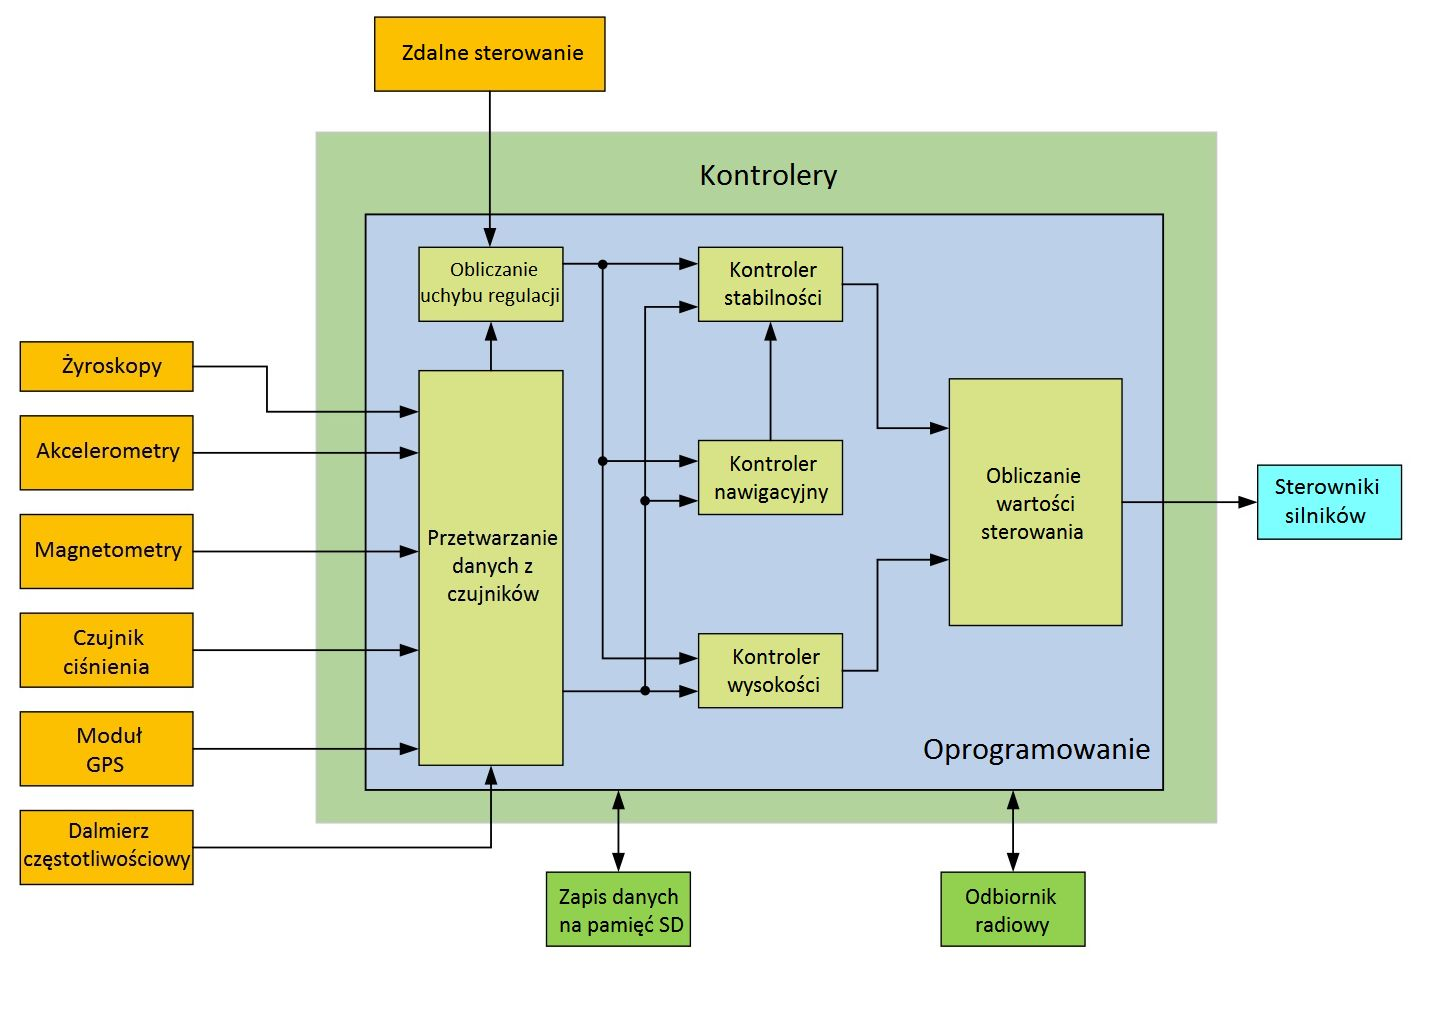
\includegraphics[width=12cm]{7_drone_platform_overview.jpg}
	\caption{Architektura programowo-sprzętowa związana z pracą autopilota \cite{Bouhali2017} }
	\label{fig:autopilot_architecture}
\end{figure} 

Rynek urządzeń typu UAV obfituje w rozwiązania oparte mikrokontrolery. 
Popularnymi autopilotami stosowanymi w komercyjnych produktach -- i przede wszystkim w ręcznie tworzonych konstrukcjach -- są: NAZA-M V2 firmy DJI oraz Pixhawk firmy 3DR. 
Oba te moduły, bazując na mikrokontrolerach ARM i dużej liczbie peryferiów, w zupełności wystarczają do zastosowań niewymagających przetwarzania dużej ilości danych, zapewniając łączność z aparaturą radiową i realizację misji opartych na predefiniowanej sekwencji ruchów. 

Nieco bardziej rozbudowane są rozwiązania wykorzystujące dwa mikrokontrolery -- jeden z~nich jest skonfigurowany w tzw. trybie „baremetal”, który oznacza uruchomienie aplikacji bezpośrednio na procesorze. 
Umożliwia to wykonywanie niskopoziomowych, krytycznych zadań, jak na przykład stabilizacja lotu uwzględniająca sterowanie pracą silników i pomiar wartości z czujników. 
Na drugim mikrokontrolerze uruchomiony jest system operacyjny, który stanowi platformę dla aplikacji wysokopoziomowych -- takich jak algorytmy planowania trasy, stereowizja czy śledzenie celu. 
Jedną z takich komercyjnych platform jest „MikroKopter” stworzony przez firmę HiSystems GmbH \cite{MikroKopter}.

Układy rekonfigurowalne, w miarę postępu technologicznego, stają się godną uwagi alternatywą -- pomimo często wyższej ceny oferują konkurencyjną wartość poboru mocy i niezrównanie szybszą prędkość działania algorytmów. 
Szczególnie, jeśli podczas ich implementacji uwzględni się możliwość zrównoleglania obliczeń. 

\section{Układy rekonfigurowalne w roli autopilota platformy UAV}

Przewaga układów rekonfigurowalnych okazuje się być widoczna już w przypadku zadania stabilizacji, a przykładem może być projekt \cite{Eizad}, w którym częstotliwość pracy regulatora PI dla osi obrotu w układzie FPGA osiągnęła wartość $4.3$MHz, w porównaniu z $0.71$MHz dla rozwiązania programowego na mikrokontrolerze ARM7. 
Prawdziwym przełomem okazały się być układy SoC, które zintegrowały część procesorową i konfigurowalną, i w efekcie dały sporą swobodę w sposobie realizacji projektu autopilota.
Zespół badawczy odpowiedzialny za opisany wyżej projekt wykorzystał układ Zynq w projekcie kolejnego drona, gdzie w części konfigurowalnej (PL -- ang. programmable logic) zaimplementowano regulację PID wymaganej do stabilizacji urządzenia, a niezależnie podejście programowo-sprzętowe pozwoliło zrealizować implementację algorytmu planowania ruchu \cite{Eizad2}. %TODO 2 objaśnić PL %ODP OK
Z kolei dla konstrukcji opisanej w publikacji \cite{Schlender}, najważniejsze zadania rozdzielono pomiędzy 3 procesory w układzie Zynq: 2 z nich, softprocesory Microblaze, odpowiadały za stabilizację, a wyższa warstwa zadań związanych ze zdefiniowaną misją realizowana była w części procesorowej (PS -- ang. processing system) opartej o architekturę ARM. %TODO 2 objaśnić PS %ODP OK

Istotnym aspektem pracy autopilota powinna być możliwość zapewnienia odpowiedniego interfejsu komunikacji z szeregiem wykorzystywanych czujników. 
Układy rekonfigurowalne nie tylko udostępniają ogromną liczbę wejść i wyjść, ale są też często wyposażone w sprzętowe kontrolery dla popularnych interfejsów. 
Ponadto, w przypadku ich niewystarczającej liczby istnieje możliwość sprzętowej implementacji własnego kontrolera. 
Przede wszystkim jednak, układ rekonfigurowalny pozwala przetworzyć otrzymane wartości w sposób bardziej złożony, niż pozwalałaby na to moc obliczeniowa mikrokontrolera. 
W publikacji \cite{MEMS} opisano implementację sprzętową cyfrowego kontrolera dla żyroskopów MEMS, który poprzez kwadraturową demodulację sygnału wejściowego i wykorzystanie równolegle pętli synchronizacji fazy (PLL) i automatycznej regulacji wzmocnienia (AGC) poprawia dokładność działania czujnika.

Kolejnym, bardzo ważnym zadaniem autopilota jest estymacja stanu, polegająca na kompensowaniu wszelkich zakłóceń pochodzących z pomiarów. 
Jest ona najczęściej realizowana w formie filtru Kalmana. 
Jedna z publikacji \cite{SohKalman} opisuje sprzętowo-programową implementację bezśladowego filtru Kalmana (UKF -- \textit{Unscented Kalman Filter}), której osiągi i zużycie zasobów są konfigurowalne poprzez zdefiniowanie liczby tzw. Bloków Przetwarzania (w liczbach: 1,2,5,10). 
Algorytm uruchomiony na urządzeniu Zynq XC7Z045 osiągał ponad dwukrotnie większą prędkość działania w porównaniu z rozwiązaniami programowymi i zużywał mniej energii (131mW dla konfiguracji z pojedynczym Blokiem). 

Ostatnim aspektem pracy autopilota jest generacja sygnałów sterujących silnikami. 
W~dronach najchętniej montowane są bezszczotkowe silniki prądu stałego, których poprawne działanie wymaga kontrolera sterującego odpowiednim przepływem prądu w uzwojeniach.
Zastosowanie układu FPGA pozwala nie tylko generować sygnały PWM wysyłane do kontrolerów prędkości (ESC), ale realizować ich funkcję z pomocą niezależnego obwodu dostarczającego zasilanie. 
Drugą formę rozwiązania zaprezentowano w pracy \cite{ESC}. 
Dzięki niemu osiągnięto wyższą częstotliwości pracy ($12.5$MHz) niż dla tradycyjnego urządzenia ESC ($50$Hz), w efekcie tworząc bardziej responsywną maszynę.

Powyższe rozważania przedstawiają potencjał, jaki osiągnąć mogą autopiloty bazujące na układach rekonfigurowalnych -- co więcej, jednostki tego typu są już dostępne w sprzedaży. %TODO 2 - to "jednak" dziwnie tutaj brzmi
Jedna z nich steruje quadrotorem „Phenox” \cite{Konomura}, w którym część konfigurowalna układu z rodziny Zynq jest odpowiedzialna za generację sygnałów PWM sterujących silnikami, odbiór informacji z czujników oraz przetwarzanie obrazu i dźwięku.
Kolejny, ważny przełom został osiągnięty przez firmę Aerotenna, która w 2016 roku rozpoczęła produkcję autopilotów kompatybilnych z niezwykle popularnym oprogramowaniem Ardupilot. 
Pierwszym z urządzeń był „OcPoc”, z układem Zynq-7000 firmy Xilinx. 
Kilka miesięcy później firma rozszerzyła portfolio o „OcPoC-Cyclone”, którego sercem został układ Intel FPGA Cyclone V \cite{Aerotenna}.
%TODO 2 a podali skąd taka zmiana Xilinx -> Intel ? %ODP Nie ma zmiany, to jest niezależny produkt (pewnie dla fanów pracy z określonym środowiskiem)

\section{Układy rekonfigurowalne w systemach wizyjnych dla platformy UAV}

Inną grupę rozwiązań stanowią układy realizujące kontrolę wysokiego poziomu, czyli wykorzystanie dodatkowych informacji w celu zapewnienia określonego poziomu autonomiczności.
 
\subsection{Zadanie detekcji i śledzenia}
Jednym z podstawowych sposobów przetwarzania materiału wideo jest ekstrakcja jego cech w celu detekcji, klasyfikacji i śledzenia obiektów oraz utrzymywania orientacji kamery. 
W publikacji \cite{RHOG} porównano dwie grupy algorytmów:
\begin{itemize}
	\item algorytmy detekcji cech: SIFT, FAST, STAR, SURF, ORB, HCD, D-HCD
	\item algorytmy opisu cech: SIFT, FEAK, BRIEF, SURF, ORB, HOG, R-HOG.
\end{itemize} 

Następnie w oparciu o algorytmy D-HCD oraz R-HOG stworzono zintegrowany system w układzie Zynq, który na podstawie analizy cech obrazów pochodzących z dwóch kamer ($1080\times 1920$ @ $30$fps) został wykorzystany w zadaniu trójwymiarowego śledzenia scen -- ale może sprawdzić się również w zadaniu śledzenia obiektów, multimodalnej rejestracji obrazów lub generowaniu struktur 3D na podstawie ruchu. 
%TODO 2 a konktrestnie to co on robił ? %ODP doprecyzowano
System z powodzeniem poddano testom na materiałach zarejestrowanych w trakcie lotu, a przy zapotrzebowaniu na moc na poziomie $4$W, częstotliwości odświeżania $30$Hz i opóźnieniu wynoszącym mniej niż $3$ klatki obrazu, deklasuje rozwiązanie uruchomione na laptopie z 8-rdzeniowym procesorem Intel i7 2.8GHz, na którym częstotliwość pracy uruchomionego algorytmu to zaledwie ok. $2$Hz.

Inna praca \cite{FIRE} opisuje system detekcji ognia i ludzi na podstawie obrazów rejestrowanych na dużej wysokości (około 2km). 
W obu przypadkach przetwarzanie dotyczy obrazów wizyjnych oraz termowizyjnych. 
Na takich materiałach rzeczywista odległość pomiędzy środkami dwóch sąsiednich pikseli wynosi $12$cm--$25$cm, zatem osoby znajdujące się na ziemi będą przedstawione za pomocą kilku pikseli.

Detekcja ludzi wymaga rozszerzenia analizy o kształt i wielkość cieni oraz charakter ruchu. 
Wykorzystywane są tu dwa rodzaje obszarów: jeden z nich związany jest z wykrywaną osobą; jest odpowiedzialny za odrzucenie obiektów, których rozmiar nie odpowiada oczekiwanej uśrednionej wielkości człowieka na obrazie. 
Dodatkową referencję stanowi obraz termowizyjny, gdzie informacja o wydzielanym cieple w określonym miejscu może zwiększyć prawdopodobieństwo obecności człowieka. 
Drugi obszar reprezentuje cień osoby, którego kierunek powinien być związany z pozycją słońca w danej lokalizacji i określonym momencie dnia. 
Informacje te można uzyskać poprzez komunikację z urządzeniami działającymi na dronie: GPS i kompasem. 
Parowanie obszarów obu typów pozwala wykryć osoby na obrazie.

Detekcja ognia polega na wykryciu dużej różnicy w temperaturach pomiędzy obszarem ogarniętym pożarem a jego tłem. 
Obszar taki jest następnie klasyfikowany pozytywnie lub negatywnie (wykorzystywany jest SVM) w oparciu o wektor cech związanych ze zmianami chromatyczności badanego obszaru. %TODO 2 klasyfikowany, klasyfikacje... %ODP OK
Autorzy pracy opisują układy rekonfigurowalne jako najlepszą platformę do realizacji systemu detekcji  -- tak ze względu na pobór mocy, wymiary, jak i moc obliczeniową przewyższającą wydajność procesorów wielordzeniowych.
\begin{figure}[h]
	\centering
	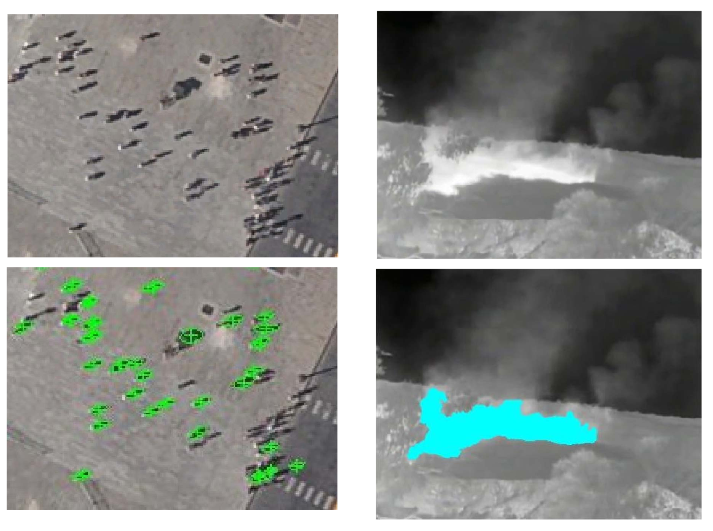
\includegraphics[width=12cm]{fire.png}
	\caption{Przykładowa detekcja ludzi (po lewej) i ognia \cite{FIRE}}
	\label{fig:fire}
\end{figure}

\subsection{Zadanie omijania przeszkód}

Systemy ostrzeżenia przed kolizją lub omijania przeszkód stają się powoli standardowym elementem wyposażenia dronów. Są one niezastąpione w sytuacji, gdy użytkownik traci maszynę z pola widzenia. 

Jedną z najczęściej rozważanych realizacji takiego systemu na platformach latających jest wykorzystanie stereowizji. 
Jej działanie polega na wyznaczeniu współrzędnych punktów sceny trójwymiarowej na podstawie obrazów uzyskiwanych za pomocą co najmniej dwóch kamer, co w efekcie umożliwia określenie odległości od przeszkód lub celów. 
Opisana w pracy \cite{STEREOVISION} implementacja algorytmu SGM (Semi-Global Matching) w układzie FPGA (XC7A100T) pozwoliła utworzyć mapę dysparycji w oparciu o obraz o parametrach $480\times 752$ @ $60$fps. 
Przetworzone dane są przechwytywane przez procesor wykorzystywany zazwyczaj w smartfonach (Samsung Exynos 4412 SoC) i zapisywane w pamięci DDR2. 
Praca ta została później wykorzystana na małej platformie UAV \cite{STEREOVISION2}, gdzie spełniała rolę systemu omijania przeszkód o niskiej latencji (poniżej $2$ms).
\begin{figure}[h]
	\centering
	\captionsetup{justification=centering,margin=1cm}
	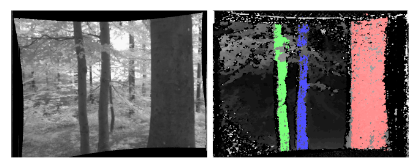
\includegraphics[width=13cm]{stereovision.png}
	\caption{System omijania przeszkód \cite{STEREOVISION2}. Po lewej wejściowy obraz w skali szarości, po prawej mapa dysparycji}
	\label{fig:stereovision}
\end{figure}

Kolejnym rozwiązaniem jest system detekcji linii zasilania \cite{STEREOVISION3}. 
W przypadku małych statków powietrznych, latających zazwyczaj na wysokości kilku, kilkunastu metrów, istnieje zwiększone ryzyko kolizji platformy UAV z instalacją elektryczną. 
Opracowany system wykorzystuje obraz stereowizyjny, poddając go równolegle transformacie Censusa oraz transformacji Top-Hat i określa stopień (koszt) dopasowania pomiędzy obrazami. %TODO 2 ale to chodzi o stereo -> tak wnoskuje.... %ODP Tak
Agregacja kosztów jest obliczana z uwzględnieniem obszaru wsparcia o krzyżowej postaci (eng. cross-based support region). %cross-based support region, nie mogłem znaleźć dobrego tłumaczenia
%TODO 2 - dac eng. %ODP OK
Po nieznacznej korekcie informacje są zapisywane w dwuportowej pamięci RAM i przekazywane do niezależnego procesora sygnałowego, który odpowiada za wyższą warstwę logiczną i realizuje funkcje decyzyjne.  
%TODO 2 - a doczytał Pan na jakies zasadzie to się dzieje ? %ODP w dokumencie nie opisano nic poza tym
Przetworzone informacje są ponownie przekazywane poprzez RAM do kontrolera wideo, który generuje obraz wyjściowy z wysegmentowanymi obszarami.
\begin{figure}[h]
	\centering
	\captionsetup{justification=centering,margin=1cm}
	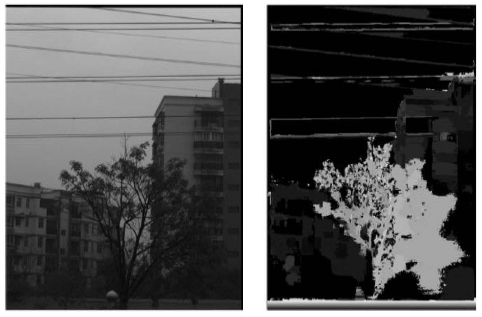
\includegraphics[width=12cm]{line_detection.png}
	\caption{Przykład systemu detekcji linii zasilania zrealizowanego w \cite{STEREOVISION3}. Po lewej wejściowy obraz, po prawej mapa dysparycji}
	\label{fig:line_detection}
\end{figure}

\subsection{Zadanie lokalizacji drona}
Inna praca \cite{Chenini} opisuje metodę estymacji pozycji drona w oparciu o obraz z kamery zamontowanej na statku powietrznym i skierowanej pionowo w dół. 
Pozwala ona wspomóc system nawigacyjny podczas lotu w utrudnionych warunkach (obniżających skuteczność np. GPS). 
Pierwszym krokiem jest określenie punktów zainteresowań -- wykorzystuje się w tym celu metodę Harrisa do wykrycia narożników, a następnie ZNCC (ang. Zero-mean Normalized Cross-Correlation) do określenia podobieństwa pomiędzy kolejnymi obrazami. %TODO 2 rozwinąć skrót ZNCC
Otrzymany zestaw informacji zawiera sporo nieprawidłowo skorelowanych par. 
Korekcja jest dokonywana w trakcie działania metody RANSAC (ang. Random Sample Consensus) opartej o algorytm Levenberga-Marquardta. %TODO 2 rozwinąć RANSAC i na tym bym skończył, bo co tu ma epipolarna do rzeczy ? %ODP OK
Implementacja systemu uwzględniała przeniesienie stworzonego wcześniej modelu programowego do części PS i stworzenie sprzętowego akceleratora dla detektora Harrisa. 
Wymiana informacji jest realizowana przez port ACP, który zapewnia bezpośredni dostęp do pamięci cache procesora. 
Ostatecznie, porównano sposoby implementacji detekcji narożników metodą Harrisa. 
Okazuje się, że dla podejścia programowego etap ten trwa ponad $750$ms, podczas gdy sprzętowa implementacja skraca ten czas do zaledwie $173$ms.

%TODO 2 - przegląd OK. Jakby się Panu udało w artykułach odszukać np. reprezentatywane zdjęcia i je tu zmieścic to już byłoby bardzo ekstra
% !TeX spellcheck = pl_PL

\chapter{Śledzenie obiektów}
\label{cha:sledzenieObiektow}

Zadanie śledzenia obiektów jest zagadnieniem z dziedziny przetwarzania obrazów. Polega na zachowaniu ciągłości analizy ruchu obiektów i zapewnieniu ich obecności w polu widzenia kamery. W praktyce wyznacza się punkt na rejestrowanym obrazie (wartość zadaną) i steruje pozycją oraz orientacją kamery w taki sposób, by jego odległość od śledzonego obiektu (również reprezentowanego przez punkt) była jak najmniejsza. Systemy wizyjne tego typu znajdują zastosowanie m.in. w rozpoznawaniu zachowań ludzi, wykrywaniu kolizji z pieszymi (systemy ADAS), weryfikacji pracy urządzeń przemysłowych czy nawet śledzeniu pojazdów na polu walki.
%TODO rozpoznawania zachowania twarzy dziwnie brzmi. Ogólnie lepsze przykłady. Z ADAS kolizja z pieszym, nawet wojskowe na polu walki śledzenie pojazdów. $ODP OK
\section{Koncepcja systemu śledzenia obiektów}
\label{sec:koncepcja}
Realizacja projektu śledzenia obiektów dla potrzeb nawigacji bezzałogowego statku powietrznego dotyczy detekcji osoby w postawie stojącej. Wymagane było tu zdefiniowanie kilku założeń:
\begin{itemize}
	\item detekcja osoby znajdującej się jedynie w bezpośrednim otoczeniu drona, wewnątrz okręgu o promieniu do 7 metrów
	\item śledzenie poprzez ruch całej platformy -- kamera jest nieruchoma, a jej pozycję dodatkowo stabilizuje gimbal kompensując wychylenia drona,
	\item śledzenie w przestrzeni trójwymiarowej, z zadaną pozycją:
	\begin{itemize}
		\item przesunięcie względem osoby: $0$m, tj. osoba powinna znajdować się w centrum obrazu rejestrowanego przez kamerę
		\item wysokość: około $1.5$m od ziemi
		\item odległość: około $4$m od osoby
	\end{itemize} 
	\item automatyzacja misji - do zadań użytkownika należy jedynie wydanie rozkazu startu z ziemi i zakończenia pracy, skutkującego lądowaniem
	\item możliwość awaryjnego przejęcia manualnej kontroli nad dronem
	\item brak funkcjonalności, która zachowałoby ciągłość detekcji w przypadku pojawienia się drugiej osoby w otoczeniu głównego celu
\end{itemize}

%TODO Brakuje tu takiego rozdziału przedstawiającego koncepcję co Pan chce zrobić. Częściowo będzie to we wstępnie, ale raczej pobieżnie. Wydaje mi się, że dobrze by było w tym rozdziale opisać koncepcję systemu (rysunek), drona i potem przejść do omówienia poszczególnych komponentów. %ODP OK
Dodatkowym warunkiem było oparcie prac na konstrukcji opisanej w kolejnych podrozdziałach.

\subsection{Platforma UAV}
Platforma, na której realizowany jest projekt, składa się z następujących elementów:
\begin{itemize}
	\item typ obiektu: hexacopter (rama DJI F550),
	\item rodzaj śmigieł: wzmocnione śmigła o oznaczeniu 9050, czyli o średnicy śmigła równej $9.0"$ ($~22.86$cm) oraz skoku śmigła $5.0"$ ($~12.7$cm).,
	\item silniki: DJI 2312/960KV sterowane kontrolerami 420 LITE,
	\item zasilanie: czterokomorowa bateria LiPo o nominalnym napięciu $14.8$V (maksymalnym $16.8$V) oraz o pojemności $6450$mAh,
	\item kamera: Xiaomi Yi,
	\item gimbal: Tarot T-2D,
	\item aparatura radiowa: FrSky Taranis X9D Plus,
	\item odbiornik: FrSky X8D,
	\item autopilot: 3DR Pixhawk.
\end{itemize}

Wybór komponentów, montaż platformy i jej kalibracja były częścią tej pracy i w ramach projektu SKN AVADER były dofinansowane ze środków Grantu Rektorskiego AGH 2015 oraz funduszy wydziału EAIiIB.
%TODO do rozdziału 1 %ODP OK
%TODO napisać wprost, że wybór komponentów, montaż itp. były a) elementem tej pracy, b) też że projektem rektorskim SKN AVADER. %ODP

\subsection{Autopilot}

Każdy dron byłby bezużyteczną konstrukcją, gdyby nie serce maszyny -- tzw. autopilot. 
W tym przypadku postanowiono wykorzystać urządzenie Pixhawk. 
Jest to zgodny ze standardami przemysłowymi moduł na otwartej licencji, stworzony przy współpracy z firmą 3D Robotics oraz ArduPilot Group. 
Posiada następujące parametry:
\begin{itemize}
	\item procesor Cortex-M4F taktowany zegarem 168 MHz,
	\item sensory: trzyosiowy akcelerometr, żyroskop, kompas magnetyczny, barometr i zewnętrzny GPS,
	\item slot na kartę microSD,
	\item możliwość połączenia peryferiów (interfejsy: UART, I2C, CAN),
	\item 14 wyjść PWM (8 głównych z zabezpieczeniami + 6 dodatkowych).
\end{itemize}

\begin{figure}[h]
	\centering
	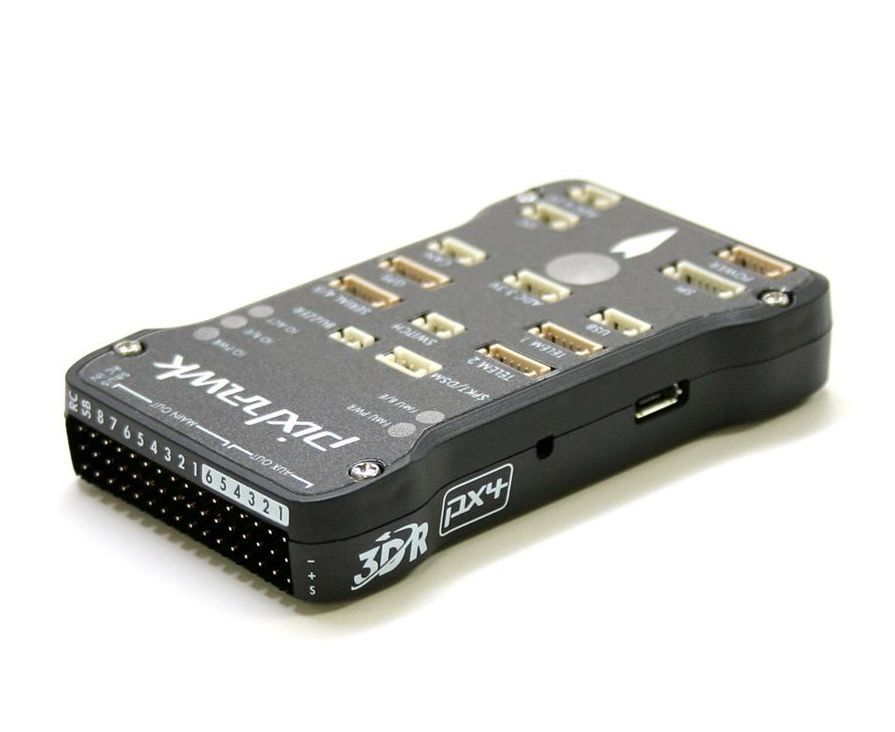
\includegraphics[width=8cm]{5_pixhawk.jpg}
	\caption{Autopilot Pixhawk -- widok na panel główny oraz we/wy PWM}
	\label{fig:pixhawk}
\end{figure}

Powyższy sprzęt jednak nie jest w pełni skonfigurowany do pracy po wyjęciu z pudełka -- szczególnie, że jako produkt uniwersalny, bywa montowany na konstrukcjach o szerokim rozrzucie parametrów. 
Może zapewnić sterowanie śmigłowcom (tzw. multicopterom), samolotom modelarskim oraz nawet łazikom. %TODO mam wątpliwość, czy słowo "kopter" jest poprawne. Skoro helikopter jest niepoprawny (był taki słynny przetarg..) to trzeba śmigłowiec. %ODP OK, do nawiasu wrzucono potoczną nazwę.
W przypadku dwóch pierwszych grup konfiguracja wiąże się ze zdefiniowaniem odpowiedniej liczby śmigieł i ich rozstawienia, typu aparatury radiowej oraz zewnętrznych urządzeń geolokalizacyjnych. 
Tę dość dużą elastyczność mogą zapewnić dwa główne systemy, które są wczytywane z pamięci SD i pracują w czasie rzeczywistym. 
Dedykowany, PX4 Flight Stack jest stworzony przez twórców modułu, oraz ArduPilot Copter (ArduCopter) -- niezależny, otwarty system, który został dostosowany do platformy Pixhawk z wykorzystaniem dostępnych narzędzi deweloperskich. 
Ze względu na większą bazę użytkowników i dojrzałość projektu, wybrano drugie rozwiązanie.

\subsection{Integracja urządzeń na platformie UAV} %TODO średni tytuł %ODP OK

Zbudowanie drona w oparciu o gotowe komponenty nie jest zadaniem skomplikowanym. 
Jednak z uwagi na wymagania projektu (opisane w \ref{sec:koncepcja}), należało dokładnie przemyśleć jego przebudowę. Rysunek \ref{fig:drone_photo} przedstawia zdjęcie zmodyfikowanej, gotowej do lotu platformy. %TODO przerobić zdanie, że z uwagi na wymagania projektu - które powinny być opisane wcześniej. %ODP OK
Z kolei schemat \ref{fig:architecture} opisuje połączenia pomiędzy urządzeniami na platformie UAV.  %TODO arch. sygnałową - dziwne określenie %ODP OK 
\begin{figure}[h]
	\centering
	\captionsetup{justification=centering,margin=1cm}
	\hspace*{0cm}
	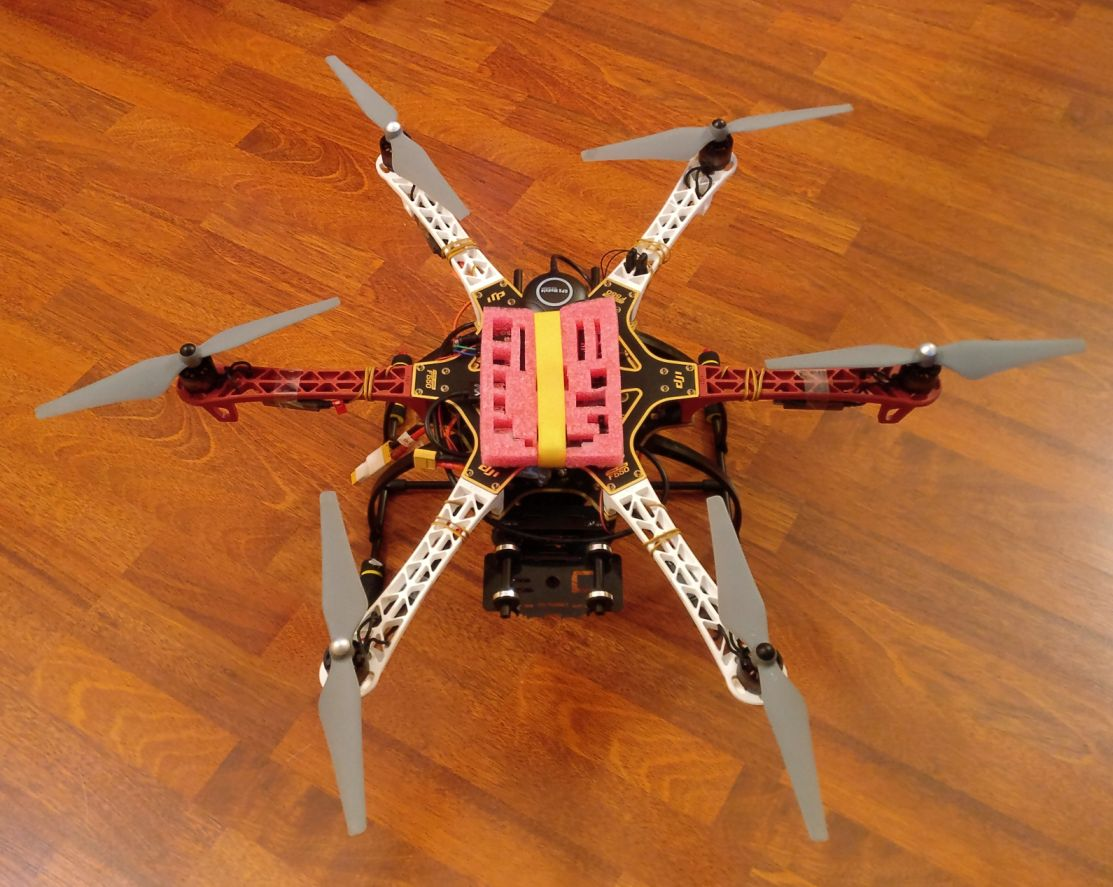
\includegraphics[width=14cm]{5_drone_photo.jpg}
	\caption{Dron po niezbędnych modyfikacjach. Pod gąbką ochronną znajduje się układ PYNQ}
	\label{fig:drone_photo}
\end{figure}
\begin{figure}[]
	\centering
	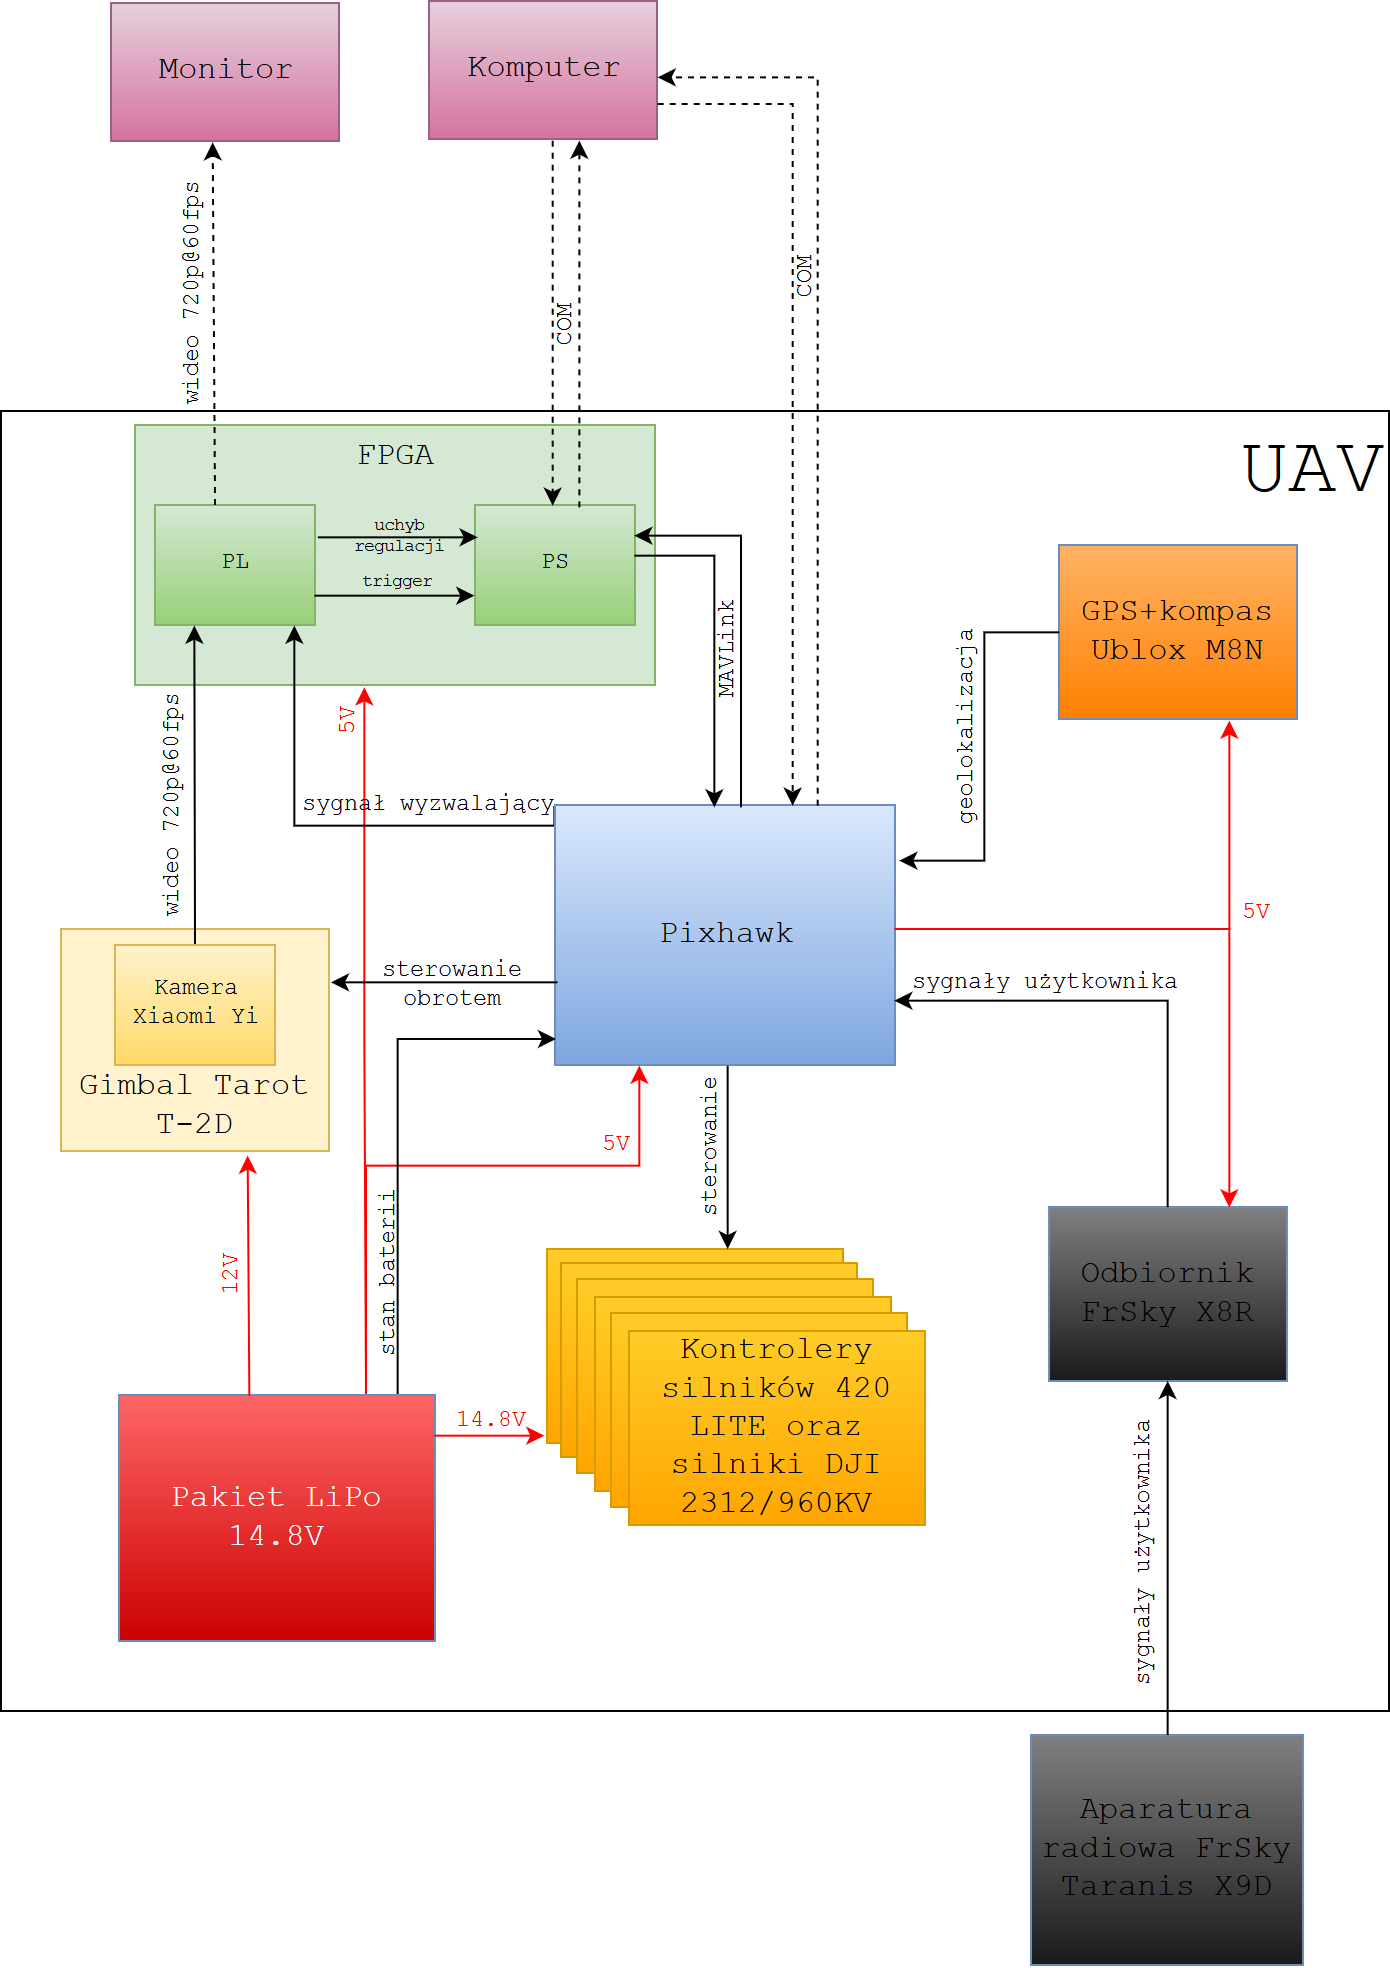
\includegraphics[width=15cm]{5_drone_architecture.png}
	\caption{Relacje pomiędzy urządzeniami na platformie UAV}
	\label{fig:architecture}
\end{figure}
Linie czerwone określają dystrybucję zasilania z zamontowanej baterii (pominięto konwertery napięcia), natomiast linie czarne opisują propagację sygnałów pomiędzy urządzeniami. Dodatkowo, liniami przerywanymi zaznaczono sygnały opcjonalne wykorzystywane w trakcie naziemnej analizy systemu. Porty szeregowe komputera służą do komunikacji z konsolą zaimplementowaną na układzie Zynq, oraz do konfiguracji autopilota poprzez aplikację MISSION Planner.


%TODO brakuje omówienia rysunku. Trzeba go po prostu opisać w tekście. %ODP OK

%TODO Brak referencji w txt. "skrywa" się potoczne. %ODP OK

%TODO co to znaczy komputer w trakcie implementacji ? %ODP zamieniono linię na przerywaną (komputer jest opcjonalnie podłączany na ziemi w celu komunikacji z układami)


%Generalnie nie mam pomysłu na to, gdzie wrzucić powyższe informacje związane z HW.
%---------------------------------------------------------------------------

\section{Rodzaje algorytmów śledzących}
\label{sec:algorytmySledzace}

Algorytmy śledzenia można umieścić w 4 głównych kategoriach utworzonych ze względu na metodę identyfikacji śledzonego obiektu na obrazie. 
Wyróżnia się metody:
\begin{itemize}
	\item różnicowe,
	\item częstotliwościowe,
	\item gradientowe,
	\item korelacyjne.
\end{itemize}

Ponadto, istnieje również podstawowy podział na sceny stacjonarne i ruchome. 
Wykorzystanie kamery stacjonarnej jest stosunkowo proste w realizacji i nie wymaga dużego nakładu obliczeniowego (do głównych czynności należy separacja tła i segmentacja obiektów ruchomych). %TODO uprościć. sceny: stancjonarne i ruchome. W pierwszym przyapdku.... (bo to co Pan napisał jest ciut zbyt zamotone) $ODP OK
W przypadku kamery posiadającej stopnie swobody, pomiędzy obecną i kolejną klatką obrazu zmianie ulec mogą wartości wszystkich pikseli. %TODO wartości wszystkich pikseli $ODP OK
Wyklucza to stosowanie algorytmów opartych o wyodrębnianie tła. 
Dodatkowo, jakikolwiek ruch kamery może zmieniać położenie obiektu i jego wielkość na obrazie - wymusza to wybór zdecydowanie bardziej złożonych obliczeniowo metod. %TODO może zmieniać (bo też może np. śledzić kamera obiekt i wtedy ruch będzie wolniejszy) $ODP racja, OK

\subsection{Algorytmy różnicowe}

Jest to grupa metod, które działają w oparciu o obraz różnicowy, powstały w wyniku odjęcia bieżącego obrazu od poprzedniej klatki lub wcześniej wygenerowanego modelu tła. %TODO modelu tła $ODP OK
Pozwala to na wyodrębnienie obszarów, gdzie nastąpiła zmiana, która zwykle związana jest z ruchem. %TODO, która zwykle związana jest z ruchem. $ODP OK
W celu wyeliminowania szumu (minimalnych zmian w wartościach pikseli) stosuje się progowanie \cite{Rosin}. 
Uzyskuje się maskę binarną - piksele nieruchome (0) i ruchome (1). 
Analizując taką informację, możliwe jest wyznaczenie nowego położenia obiektu i zdefiniowanie przesunięcia, które nastąpiło pomiędzy klatkami. 

Największą zaletą metod różnicowych jest ich prostota w zrozumieniu oraz implementacji, mająca również efekt w niskiej złożoności obliczeniowej. 
Z drugiej jednak strony, tak proste metody bywają zawodne w przypadku większych zakłóceń i ruchu w sąsiedztwie obiektu, błędnie interpretowanego jako właściwe przesunięcie. 
Ponadto, zastosowania tych metod ograniczają się jedynie do obrazów rejestrowanych za pomocą kamery stacjonarnej, co eliminuje je z dalszych rozważań w tej pracy. 

%TODO No dobra. A co jak będą dwa obiekty ? %ODP Pytanie o tę sekcję, czy ogólnie? Jeśli w moim projekciebędą dwie osoby, to algorytm wybierze "bardziej widoczną" i się jej będzie trzymał do czasu zasłonięcia jednej osoby drugą, wtedy się pewnie wysypie.

\subsection{Algorytmy częstotliwościowe}

Metody te opierają się na interpretacji obrazu w dziedzinie częstotliwości. 
Istnieją różne filtry częstotliwościowe, które pozwalają na wykrycie krawędzi - więc, odpowiednio zaimplementowane, umożliwiają również identyfikację obiektu na kolejnych klatkach wideo. %TODO może na kolejnych %ODP OK
 %TODO ale akurat Gabor raczej w dziedzinie przestrzennej %ODP OK, wykasowano
Praca w dziedzinie częstotliwości daje możliwość wykrycia przesunięć obiektu, które mogłyby zostać niezauważone w przypadku stosowania pozostałych typów metod. 
Swoją wysoką dokładność algorytmy te każą jednak opłacić nieporównywalnie większą złożonością obliczeniową, związaną z obliczeniem transformaty Fouriera i stosowaniem filtrów częstotliwościowych. %TODO każą jednak opłacić (styl !) %ODP OK

\subsection{Algorytmy gradientowe}

Działanie wspomnianych metod śledzenia obiektów opiera się na założeniu niewielkich zmian w luminancji (jasności, oświetleniu) oraz niewielkim przesunięciu obiektu pomiędzy kolejnymi klatkami obrazu. %TODO trzeba dodać niewielkim przesunięciu %ODP OK, gdzieś to musiałem zgubić
Istotą tych algorytmów jest znalezienie odpowiedniego przesunięcia obiektu pomiędzy kolejnymi klatkami, tak, aby wskaźnik jakości wynikający z podobieństwa obszarów był zminimalizowany. 
Poszukiwania obszaru można realizować globalnie, bądź na fragmencie będącym otoczeniem śledzonego obiektu. 
Algorytm realizujący obliczenia lokalnie może zawodzić w sytuacjach, gdy przesunięcia są zbyt duże i wykraczają poza obszar poszukiwań, jednak taka metodyka obniża złożoność obliczeniową całego algorytmu i znajduje swoje zastosowania w określonych sytuacjach. %TODO algorytm prowadzący... - nie personifikować...  %ODP OK
Spośród wielu algorytmów gradientowych stosowanych do śledzenia obiektów, najpopularniejszymi są MeanShift, Camshift oraz KLT. %TODO do HOG się nie zgodzę. A dodałbym jeszcze KLT. %ODP OK 

\subsection{Algorytmy korelacyjne}

Działanie tej grupy algorytmów polega na maksymalizacji funkcji korelacyjnej obliczanej na blokach pikseli. %TODO trochę powt. Działanie tej grupy algorytmów polega na maksymalizacji korealcji....%ODP OK
Podstawowym założeniem jest jeden wspólny kierunek przemieszczenia wszystkich punktów obiektu - nie jest to zatem najlepsze rozwiązanie dla innych typów ruchu. %TODO styl. nie działają.%ODP OK
Istotnym dla złożoności i wydajności parametrem przy implementacji tej grupy metod jest określenie rozmiaru obszaru poszukiwań -- w przypadku mniejszych, problemem bywa przemieszczenie obiektu poza obszar; w przypadku tych większych istnieje ryzyko znalezienia maksimum funkcji korelacyjnej, które nie odpowiada obiektowi. %TODO no i złożóność...%ODP poprawione
Zaletą metod korelacyjnych jest jednak mniejsza wrażliwość na zachodzące na siebie obiekty, co umożliwia śledzenie bardziej złożonych ruchów %TODO to jest niejasne %ODP OK poprawione, sam teraz nie wiem o co mogło mi chodzić, a to przeoczyłem przy sprawdzaniu.
Stosuje się je często, gdy obliczanie pochodnych (dla metod gradientowych) byłoby utrudnione -- przykładowo w przypadku gwałtownego ruchu obiektu lub niewystarczającej częstotliwości próbkowania sygnału wideo. %TODO ten klatkaż to potworek. czestotliwosci próbkowania sygnłaku wideo %ODP niby jest w używany przez filmowców, więc to już bardziej słownictwo zawodowe niż potoczne;) https://sjp.pwn.pl/poradnia/haslo/klatkaz;13832.html; ale zmieniłem
Jedną z najbardziej popularnych metod korelacyjnych jest BMA, często używana w kompresji wideo \cite{Aroh}.

\subsection{Algorytmy śledzenia przez detekcję}
Działanie tej grupy algorytmów polega na niezależnym wykrywaniu określonych obiektów w kolejnych klatkach obrazu. Detekcja jest oparta na ekstrakcji kilku charakterystycznych cech obiektu, na przykład kształtu. W kolejnym etapie tak stworzony deskryptor jest klasyfikowany jako obiekt lub odrzucany. Istotną wadą tych metod śledzenia jest duża wrażliwość na zmianę odległości od obiektu -- rozwiązuje się ten problem poprzez analizę kilku przeskalowanych obrazów, jednak podnosi to ogólną złożoność obliczeniową ekstrakcji cech. Odrębną kwestią są parametry klasyfikatora, uzyskiwane w procesie uczenia i mocno wpływające na efekty działania tych metod.
W skład tej grupy wchodzą m.in. algorytmy HOG, SIFT oraz SURF.
%TODO Jeszcze brakuje Panu śledzenia przez detekcję - i do tego ten HOG wchodzi. Z popluarnych metod to jeszcze filtry cząsteczkowe, choć one chyba też umykają Pana klasyfikacji.
%TODO kolejna kwestia to jednak wypadałoby powołać się na jakąś literaturę na podstawie, której Pan to opisał.

\subsection{Algorytmy śledzenia wykorzystujące filtry cząsteczkowe}
Idea działania tej grupy metod polega na przedstawieniu pozycji obiektu za pomocą zbioru losowych próbek (cząsteczek). Każda z nich związana jest z prawdopodobieństwem obecności obiektu w pozycji reprezentowanej przez tę cząsteczkę. Po otrzymaniu nowej klatki obrazu, cząsteczkom są przypisywane wagi na podstawie zgodności predykcji. Następnie odpowiednio cząsteczki z dobrym wynikiem są pomnażane, natomiast te o złych parametrach są usuwane z obliczeń.
Wydajność tej grupy algorytmów w dużej mierze zależy od liczby zdefiniowanych cząsteczek, co może mocno wpłynąć na złożoność obliczeniową.
%Nie wiem, czy mój opis jest do końca poprawny.
\subsection{Podsumowanie}

Ostatecznie w realizacji projektu postanowiono zaimplementować algorytm gradientowy: MeanShift i metodę śledzenia przez detekcję: HOG+SVM. %TODO HOG śledznie przez detekcję. Tzn. wiem, że tam korzysta się z gradientów, ale...%ODP OK
O takim wyborze zadecydowała możliwość wykorzystania obu rozwiązań dla obrazu pochodzącego z kamery ruchomej, co w przypadku pracy drona było decyzją naturalną. %TODO powt. algorytmów.%ODP OK
Mimo, że MeanShift jest algorytmem iteracyjnym (kryterium zakończenia obliczeń stanowi limit iteracji bądź uzyskanie określonej dokładności), to odpowiednie zaprojektowanie modułu obliczeniowego w FPGA pozwoli przetwarzać obraz w czasie rzeczywistym, tj. ukończyć przetwarzanie aktualnej klatki przed rozpoczęciem przetwarzania kolejnej - tak szybko, jak tylko uzyska się na jej temat komplet informacji. %TODO dodać, że przy odpowiednim zaprojektowaniu modułu obliczeniowego%ODP OK
Metoda ta charakteryzuje się dobrymi wynikami w przypadku obiektów zmieniających orientację -- jest to szczególnie przydatne w sytuacji, gdy miejscem umiejscowienia kamery jest dron -- maszyna podatna na podmuchy wiatru zmieniające chwilowo jej orientację względem obiektu. 

Z kolei zastosowanie algorytmu HOG/SVM będzie miało szczególne znaczenie w pierwotnej detekcji śledzonej postaci. Ponadto, jednoczesna analiza kilku przeskalowanych obrazów na danym obszarze pozwoli wybrać najlepszy wynik i określić na tej podstawie odległość kamery od celu  %TODO kompensowanie głębi- usunąć. Natomiast tą rolę trzeba opisać lepiej. Ale to i tak będzie miało sens tylko, jak wcześniej (zgodnie z sugestią) przecyzjie zostanie opisana koncepcja. Rola algorytmu HOG jest dwojaka. Odległość, ale też rozumiem inicjalizacja/re-inicjalizacja mean-shift (metody się uzupełniają) - no przynajmniej w teorii. %ODP Opisano
%Poprawność działania systemu wbudowanego będącego połączeniem obu algorytmów została potwierdzona testami, które zostały przeprowadzone na modelu programowym oraz na symulacjach kodu System Verilog. %TODO to zdanie to do innej cześci pracy. Tu na razie koncepcja. %ODP OK

Oba algorytmy były wcześniej implementowane w układach rekonfigurowalnych w niezależnych projektach \cite{Mazur},\cite{Patel}, \cite{Drozdz}.
%TODO Można też dodać, że oba algorytmy były wcześniej implementowane w FPGA (literatura). %ODP OK

\section{Algorytm MeanShift}

MeanShift jest algorytmem zaprezentowanym po raz pierwszy w 1975 roku przez K. Fukunagę i L. Hostetlera \cite{Fukunaga}. Jest to metoda znajdowania maksimum rozkładu gęstości na pewnym ograniczonym obszarze. Iteracyjny charakter algorytmu pozwala aktualizować położenie obszaru, przemieszczając go w kierunku maksimum i rozpoczynając ponownie analizę.

Z czasem stwierdzono, że MeanShift może znaleźć zastosowanie w systemach wizyjnych. Dla uprzednio zlokalizowanego na obrazie obszaru z obiektem należy zapisać go w postaci histogramu barw. W celu zapewnienia zbieżności histogram ten oblicza się w oparciu o postać jądra, którego wagi będą faworyzowały wartości pikseli w centrum obszaru. Pierwszy histogram pełni rolę wzorca, z którym porównywane są histogramy obszarów z kolejnych klatek obrazu (kandydaci). Dzięki odpowiedno zastosowanym wagom algorytm znajduje maksimum rozkładu gęstości (podobieństwa) i przemieszcza obszar w jego kierunku, by na nowym zestawie pikseli rozpatrzyć kolejnego kandydata.
%TODO TU by się przydało jakieś wprowadzanie i podanie źródła z literatury. %ODP OK

\subsection{Konwersja przestrzeni barw RGB->HSV}
\label{sec:rgb2hsv} %TODO chyba zły label %ODP OK

%TODO Opis mean-shift jest ~ poprawny, ale taki dość trudny do zrozumienia. Na początku trzeba w kilku zadaniach opisać o co chodzi - tak jak jest to na tym schamcie blokwoym i potem uszczegółowić. Proszę też jeszcze raz sprawdzić wzory. %ODP OK

Algorytm MeanShift użyty w procesie śledzenia wykorzystuje rozkład prawdopodobieństwa wybranej cechy na obrazie -- w tym wypadku barwy. 
Jest to składowa H z przestrzeni barw HSV (ang. \textit{Hue, Saturation, Value}). 
Domyślną przestrzenią do rejestracji i zapisu obrazów jest jednak RGB, zatem wymagana jest jej konwersja. 
O ile przestrzeń RGB reprezentowana jest przez sześcian określony parametrami 3 kolorów: czerwonego, zielonego i niebieskiego, to przestrzeń barw HSV opisywana jest przez stożek. 
Jego podstawą jest koło, którego kąt opisuje barwę (H -- \textit{Hue}). %TODO to jest barwa, kat opisuje barwę %ODP OK
Kolor czerwony jest reprezentowany przez kąty $0$\si{\degree} (lub $360$\si{\degree}), zielony przez kąt $120$\si{\degree}, a kolor niebieski przez $240$\si{\degree}. 
Promień koła barw opisuje nasycenie koloru (S -- \textit{Saturation}), zaś za moc światła białego, czyli jasność (V -- \textit{Value}) odpowiada wysokość stożka. 
Model HSV jest lepiej powiązany ze sposobem, w jaki postrzega ludzki narząd wzroku, dla którego wszystkie barwy są światłem odbitym od obiektów.
Rysunek \ref{fig:HSV_cone} przedstawia interpretację graficzną składowych przestrzeni HSV na stożku.

\begin{figure}[h]
	\centering
	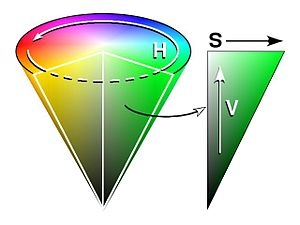
\includegraphics[width=6cm]{2_HSV.jpg}
	\caption{Stożkowa przestrzeń barw modelu HSV \cite{HSV}} %TODO  źródło obrazu (na oko wiki) %ODP OK
	\label{fig:HSV_cone}
\end{figure}

Poniższe wzory opisują sposób wyznaczenia poszczególnych składowych przestrzeni HSV w oparciu o RGB \cite{Kryjak}. Wymagają one kilku względnie złożonych operacji dzielenia.

\begin{equation}
\label{HSV_first}
V=max(R,G,B)
\end{equation}

\begin{equation}
S=\begin{cases}
\frac{V-min(R,G,B)}{V}, & V\neq0 \\
0, & V=0
\end{cases}
\end{equation}

\begin{equation}
\label{HSV_last}
H=\begin{cases}
	0, & \text{jeśli } V-min(R,G,B)==0 \\
	\frac{60(G-B)}{V-min(R,G,B)}, & \text{jeśli } V==R \\
	\frac{60(B-R)}{V-min(R,G,B)}+120, & \text{jeśli } V==G \\
	\frac{60(R-G)}{V-min(R,G,B)}+240, & \text{jeśli } V==B 
\end{cases}
\end{equation}


%TODO Można skomentować, że wymajają one operacji dzielena, która jest wzlędnie złożona. %ODP OK

\subsection{Wektor MeanShift}
\label{ssec:MS}

Istotą działania algorytmu MeanShift jest wyznaczanie maksimum funkcji gęstości w kolejnych iteracjach. 
Dla określanego obszaru obliczany jest środek ciężkości punktów, których nagromadzenie wskazuje na większy stopień podobieństwa rozpatrywanego obszaru z oryginałem. Do nowego środka ciężkości zostaje przesunięte aktualne położenie środka po zakończeniu algorytmu. %TODO trochę nie wiadomo skąd te punkty %ODP OK

To przesunięcie nosi nazwę \textit{wektora MeanShift}, który dla zbioru \textit{n} punktów $\{x_{i}\}_{i=1..n}$ oraz środka obszaru w punkcie $y_0$ może zostać zapisany jako:

\begin{equation}
\label{eq:ms1}
M(y)=\bigg[\frac{1}{n}\mathlarger{\sum\limits_{i=1}^{n}}x_i\bigg]-y_0
\end{equation}

Prostota wzoru \eqref{eq:ms1} wynika z ujednolicenia wagi dla wszystkich punktów. %TODO referencja do wzorów \eqref - dodaje nawias %ODP OK
Wprowadzając wagę punktu zależną od jego odległości od środka obszaru -- takiej, która maleje wraz z oddalaniem się od centrum), wzór \eqref{eq:ms1} można przepisać jako:

\begin{equation}
\label{eq:ms2}
M(y)=\frac{\sum_{i=1}^{n}w_i(y_0)x_i}{\sum_{i=1}^{n}w_i(y_0)}-y_0
\end{equation}
W równaniu \eqref{eq:ms2}, $w_i(y_0)$ są wagami dla poszczególnych punktów.

Rysunek  \ref{fig:ms_vector} ilustruje przykładowe wygenerowanie wektora MeanShift, gdzie niebieskim okręgiem zaznaczono obszar podlegający działaniu algorytmu. 
Wszystkie punkty mają tu jednak identyczną wagę.
\begin{figure}[h]
	\centering
	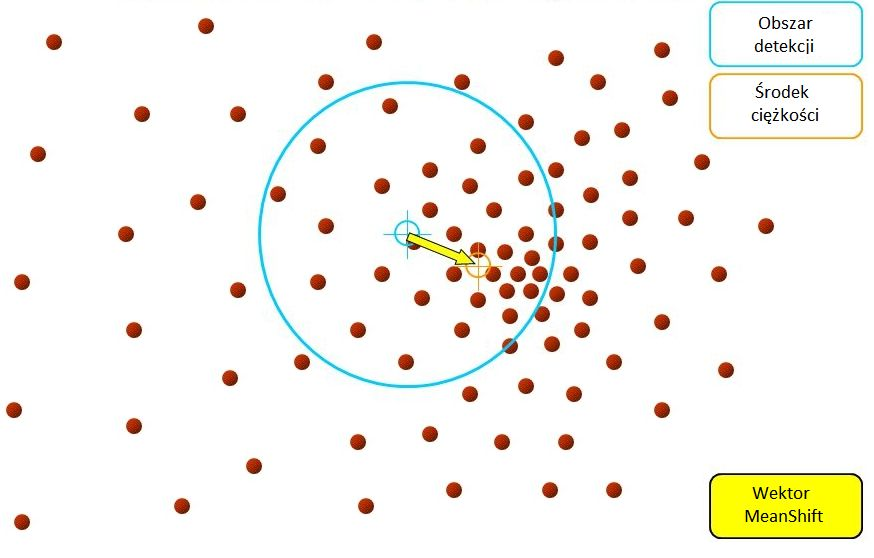
\includegraphics[width=10cm]{2_meanshift.jpg}
	\caption{Graficzna interpretacja wektora MeanShift \cite{Egorov}}
	\label{fig:ms_vector}
\end{figure}
%TODO przy tak prostym rysunku można w paint podmienić napisy na PL %ODP OK

\subsection{Jądro obszaru}

Celem wyznaczenia jądra (ang. \textit{kernel}) dla obszaru o stałej wielkości jest przypisanie najwyższej wagi punktom, które znajdują się najbliżej środka obszaru. 
Konsekwencją tego jest nadawanie znikomych wag punktom na jego brzegach. %TODO rubieże to złe słowo (brzegi) %ODP OK
Postać jądra zwykle przyjmuje klasyczne postacie gęstości rozkładów probabilistycznych: między innymi rozkładu jednorodnego (wagi jednakowe), prostokątnego, Gaussa, Cauchy'ego, Epanechnikova. 
W niniejszej pracy zdecydowano się wykorzystać jądro trójkątne ze względu na jego dobre wyniki i jednoczesną prostotę implementacji, nie bez znaczenia podczas późniejszej realizacji sprzętowej w układzie FPGA. 
Jądro takie można opisać poniższym wzorem:

\begin{equation}
\label{eq:ms3}
K(u)=\begin{cases}
1-\frac{u}{b}, & \text{jeśli }\frac{u}{b}\leq 1 \\
0, & \text{jeśli }\frac{u}{b} > 1
\end{cases}
\end{equation}
gdzie: $u$ jest odległością pomiędzy punktem a środkiem obszaru, a $b$ jest połową jego boku (zakładając, że obszarem jest kwadrat). Rysunek \ref{fig:kernel} przedstawia jądro o wymiarach 100x100 -- w punkcie (50,50) osiąga maksymalną wartość 1 (natomiast $u=0$).
\begin{figure}[h]
	\centering
	\captionsetup{justification=centering,margin=1cm}
	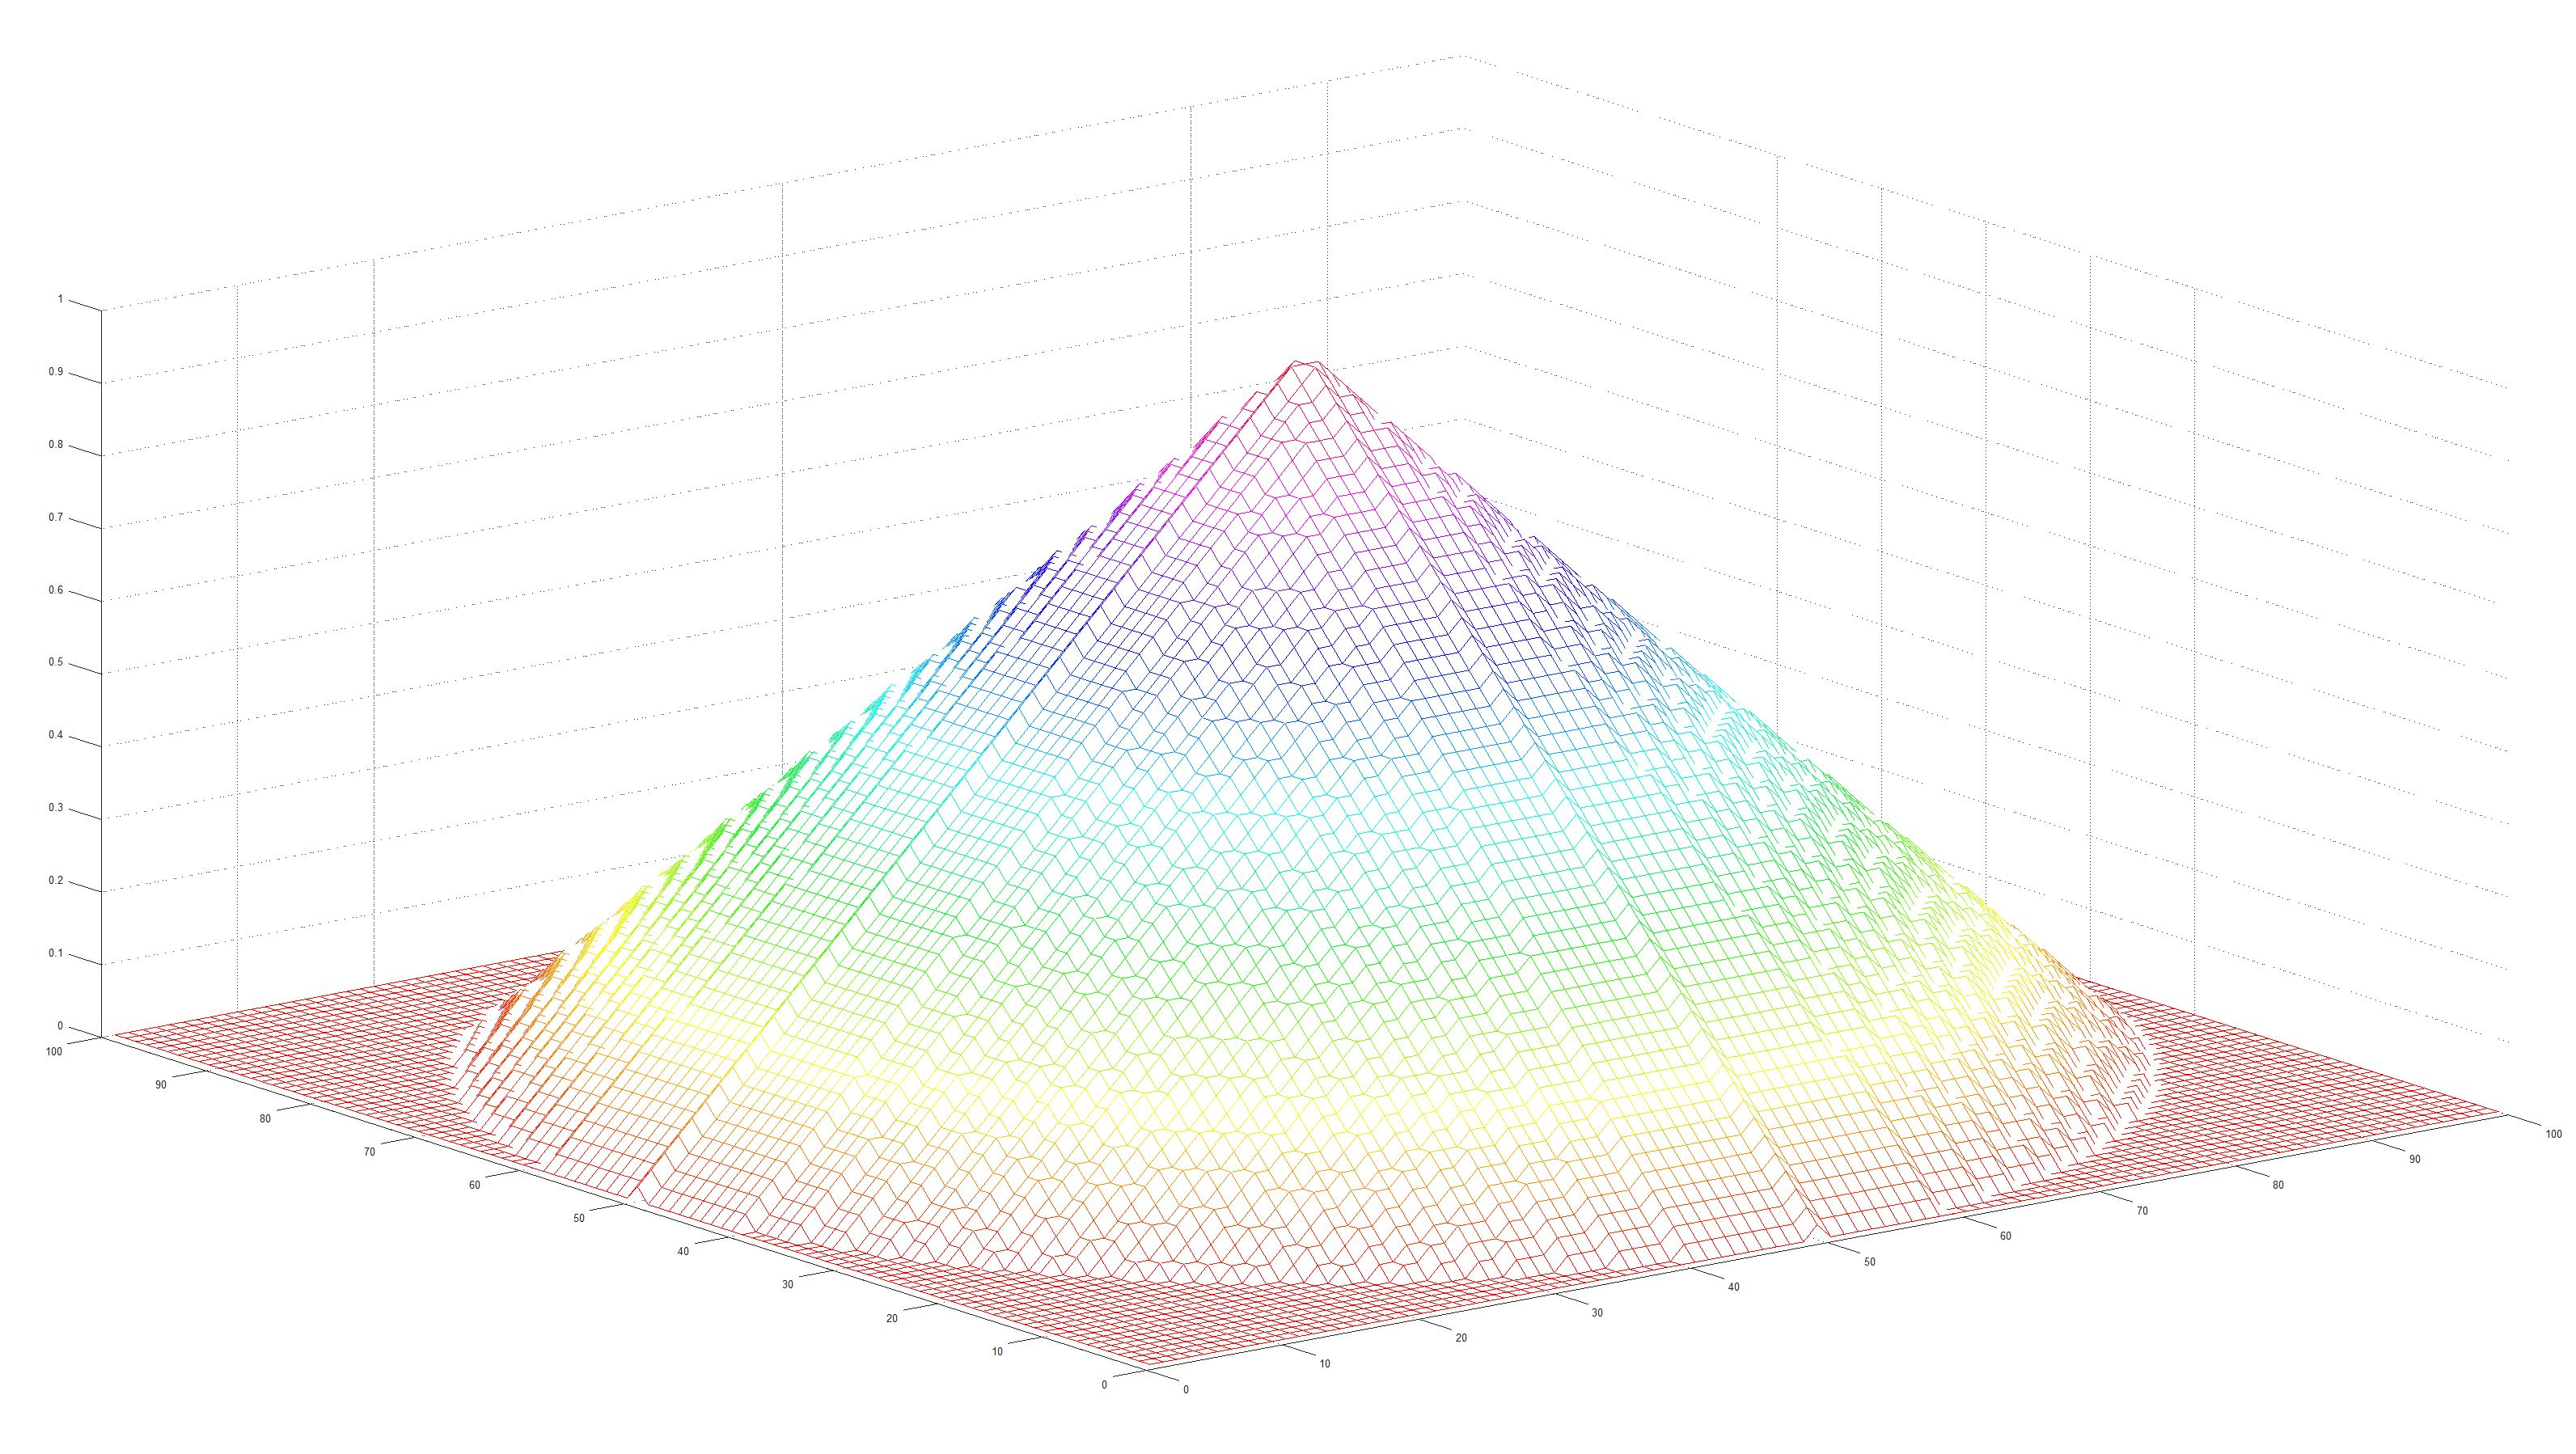
\includegraphics[width=12cm]{2_kernel.jpg}
	\caption{Jądro obszaru o wymiarach $100\times100$ (wygenerowane w programie MATLAB)}
	\label{fig:kernel}
\end{figure}
%TODO rysunek może być ciut mniejszy %ODP OK

\subsection{Gęstość jądra}
Mając zbiór $n\times n$ punktów: $\{x_{i},y_{j}\}_{i=1..n,i=j..n}$ z przestrzeni $\mathbb{R}^2$ oraz jądro $K(u)$ dla punktu centralnego $P=(x,y)$ można przedstawić funkcję oszacowania gęstości:

\begin{equation}
f(P)=\frac{1}{n^2}\sum_{i=1}^{n}\sum_{j=1}^{n}K(||P-P'(i,j)||).
\end{equation}
%TODO Nie za bardzo rozumiem dlaczego są dwa wzory... %ODP OK, usunięto nieużywany dalej wzór
Różniczkując powyższe otrzymuje się:
\begin{equation}
\label{eq:K}
\nabla f(P)=\frac{1}{n^2}\sum_{i=1}^{n}\sum_{j=1}^{n}(P-P'(i,j))K'(||P-P'(i,j)||),
\end{equation}
a po podstawieniu $g(x)$ za $-K'(x)$, wzór \eqref{eq:K} może zostać zapisany jako:
\begin{equation}
\nabla f(x)=\frac{1}{n^2}\sum_{i=1}^{n}\sum_{j=1}^{n}(P'(i,j)-P)g(||P-P'(i,j)||),
\end{equation}
%TODO tu chyba coś jest nie tak z minusem....też jedna suma uciekła... %ODP OK, walnąłem się przy przeglądaniu pracy Krzyśka Mazura
Po przekształceniu wzór może być przedstawiony jako:
\begin{equation}
\label{eq:kerms}
\begin{aligned}
\nabla f(x)= &\frac{1}{n^2}\bigg[\sum_{i=1}^{n}\sum_{j=1}^{n}g(||P-P'(i,j)||)\bigg] \cdot\\ \cdot&\bigg[\frac{\sum_{i=1}^{n}\sum_{j=1}^{n}P'(i,j)g(||P-P'(i,j)||)}{\sum_{i=1}^{n}\sum_{j=1}^{n}g(||P-P'(i,j)||)} -P\bigg],
\end{aligned}
\end{equation}
Ze wzoru \eqref{eq:kerms} można wyodrębnić człon będący gradientem jądra: $g(P)=-K'(P)$. 
Drugą jego część stanowi wektor MeanShift z wagami odpowiadającymi wartościom gradientu jądra o środku w punkcie $x$. 
Zakładając niezerowość wyrażenia $\sum_{i=1}^{n}\sum_{j=1}^{n}g(||P-P'(i,j)||)$, wektor ten może przyjąć ostateczną formę:
%TODO tu ma Pan ^2, a we wzorach nie... %ODP generalnie w źródłach podawana jest norma z ^2, co wydaje mi się dziwne - opisana przeze mnie funkcja K(||P-P'(i,j)||) zwraca zwraca wartość jądra dla danej odległości od środka [K(0)], w którym osiąga maksimum. Dziwi mnie trochę to zastosowanie kwadratu przy normie, stąd usunąłęm w swoich wzorach.
\begin{equation}
M_s(P)=\frac{\sum_{i=1}^{n}\sum_{j=1}^{n}P'(i,j)g(||P-P'(i,j)||)}{\sum_{i=1}^{n}\sum_{j=1}^{n}g(||P-P'(i,j)||)} -P.
\end{equation}

\subsection{Współczynnik Bhattacharyya}
 \label{ssec:Bhat}

Zastosowanie algorytmu MeanShift do śledzenia obiektów na materiale
wideo wymaga znalezienia zależności pomiędzy funkcjami gęstości wzorca oraz kandydata. 
W tym celu należy zestawić ze sobą oba rozkłady na przykład za pomocą współczynnika Bhattacharyya, który dla $m$-wymiarowych funkcji gęstości wzorca $q_h$ oraz obszaru-kandydata $p_h$ ze środkiem w punkcie $P$ wyraża się wzorem \cite{Comaniciu}:
\begin{equation}
\label{eq:Bhat}
\rho(P)=\sum_{h=1}^{m}\sqrt{p_h(P)q_h}
\end{equation}
Wyznaczenie przesunięcia obiektu na obrazie dla kolejnych klatek obrazu wymaga znalezienia maksymalnego współczynnika Bhattacharyya, co jest tożsame (według algorytmu) ze zidentyfikowaniem najbardziej podobnego fragmentu do oryginalnego obszaru śledzonego.

\subsection{Śledzenie}

Opisane wyżej jądro i jego gradient stanowią inicjalizację całego algorytmu i są obliczane jeszcze przed zdefiniowaniem wzorca. 
Cechą obrazu, dla której będzie liczona funkcja prawdopodobieństwa, jest kolor (H z przestrzeni barw HSV, jest to liczba z zakresu 0-359). 
Jeśli położenie piksela na obrazie wzorca oznaczone jest jako $\{x_{i},y_{j}\}_{i=1..n,i=j..n}$, niech zdefiniowana będzie funkcja $b:\mathbb{R}^2\rightarrow\{1..m\}$, która odwoływać się będzie do składowej \textit{H} danego piksela.

Barwa piksela stanowi argument funkcji prawdopodobieństwa utworzonego dla \textit{H} na danym obszarze detekcji. %TODO przede wszystkim ? %ODP OK, wykasowano
Współczynnik Bhattacharyya jest \textit{de facto} porównaniem dwóch funkcji prawdopodobieństwa (wzorca i kandydata), każdej będącej histogramem o 360 przedziałach. %TODO wymiar cech to średnio brzmi %ODP OK
Podczas obliczania prawdopodobieństwa wystąpienia określonego koloru, istotną rolę odgrywać musi wartość jądra, które zwiększa wagę pikseli znajdujących się w centrum obszaru, marginalizując znaczenie tych brzegowych -- które mogłyby być częścią zmiennego w czasie tła. 
O ile w tradycyjnym histogramie wartości przedziałów zwiększa się poprzez inkrementację, to w tym przypadku zdecydowano się na powiększenie o wartość jądra odpowiadającego położeniu piksela na obszarze 100x100.
Dla przykładowej barwy $h$, funkcja gęstości prawdopodobieństwa może być zdefiniowana jako:
\begin{equation}
q_h=C\sum_{i=1}^{n}\sum_{j=1}^{n}K(||P-P'(i,j)||)\delta[b(P'(i,j))-h],
\end{equation}
gdzie $P$ to nadal środek obszaru detekcji, a symbol $\delta$ jest deltą Kroneckera. Współczynnik $C$ odpowiada za normalizację $q_h$: $\sum_{h=1}^{m}q_h=1$.
Po przekształceniu okazuje się, że:

\begin{equation}
C=\frac{1}{\sum_{i=1}^{n}\sum_{j=1}^{n}K(||P-P'(i,j)||)} 
\end{equation}

W każdej iteracji dla kandydata wyznacza się funkcję gęstości prawdopodobieństwa. 
Uwzględniając obszar ze środkiem w punkcie $P$, wzór prezentuje się następująco:
\begin{equation}
\label{eq:density}
p_h(P)=C_k\sum_{i=1}^{n}\sum_{j=1}^{n}K(||P-P'(i,j)||)\delta[b(P'(i,j))-h] 
\end{equation}

Współczynnik $C_h$ wyznacza się podobnie, jak dla wzorca, jednak z uwgzlędnieniem położenia środka obszaru kandydata, $P$:
\begin{equation}
C_k=\frac{1}{\sum_{i=1}^{n}\sum_{j=1}^{n}K(||P-P'(i,j)||)} 
\end{equation}
Następnie należy zbadać podobieństwo obu rozkładów gęstości -- wykorzystywany jest w tym celu współczynnik Bhattacharyya, opisany w rozdziale \ref{ssec:Bhat}. Rozwijając wzór \eqref{eq:Bhat} w szereg Taylora ze środkiem obszaru wzorca równym $P_0$ można otrzymać:
\begin{equation}
\label{eq:approx}
\rho(p(P),q)\approx\frac{1}{2}\sum_{u=1}^{m}\sqrt{p_u(P_0)q_u} + \frac{1}{2}\sum_{u=1}^{m}p_u(P)\sqrt{\frac{q_u}{p_u(P_0)}}
\end{equation}
Podstawienie równania \eqref{eq:density} do powyższego wyrażenia daje:
\begin{equation}
\label{similarity_est}
\begin{aligned}
\rho(p(P),q)\approx & \frac{1}{2}\sum_{u=1}^{m}\sqrt{p_u(P_0)q_u} + \\ & \frac{C_k}{2}\sum_{i=1}^{n}\sum_{j=1}^{n}\sum_{u=1}^{m}\sqrt{\frac{q_u}{p_u(P_0)}}\delta[b(P'(i,j))-h] k(||P-P'(i,j)||)
\end{aligned}
\end{equation}
Stąd można wyodrębnić:
\begin{equation}
\label{eq:wi}
w_{i,j}=\sum_{u=1}^{m}\sqrt{\frac{q_u}{p_u(P_0)}}\delta[b(P'(i,j))-h]
\end{equation}


We wzorze \eqref{similarity_est} pierwsza składowa jest niezależna od położenia środka obszaru kandydata $P$. 
Maksymalizując funkcję podobieństwa, należy skupić się na poszukiwaniu największej wartości drugiego członu. 
Wykorzystując wektor MeanShift z rozdziału \ref{ssec:MS} z wagami równymi wartościom funkcji podobieństwa wzorca i kandydata oraz wzór \eqref{eq:wi}, dla każdej klatki obrazu i w każdej iteracji należy wyliczyć aktualne położenie obszaru w oparciu o względne przesunięcie dane poniższym wzorem.

\begin{equation}
\label{eq:position}
\Delta P=\frac{\sum_{i=1}^{n}\sum_{j=1}^{n}P(i,j)\cdot w_{i,j}\cdot g(P-P'(i,j))}{\sum_{i=1}^{n}\sum_{j=1}^{n}w_{i,j}\cdot g(||P-P'(i,j)||)}
\end{equation}

\subsection{Warunki zakończenia algorytmu}

W przypadku algorytmu iteracyjnego konieczne jest zdefiniowanie celów, które należy osiągnąć. 
Uzyskanie całkowitego podobieństwa pomiędzy wzorcem i kandydatem w zmiennej sekwencji obrazów jest w realnych warunkach nie do uzyskania. %TODO powt. osiągnąć. %ODP OK
Chcąc przetwarzać obraz w czasie rzeczywistym, należy zakończyć przetwarzanie klatki przed momentem, w którym dane z następnej będą gotowe. 
Stąd dwa podstawowe warunki zakończenia algorytmu to:
\begin{enumerate}
	\item numer iteracji == maksymalna liczba iteracji
	\item $||P_{n_m}-P_{n_{m-1}}||<\epsilon$, %TODO =0 czy mniejsze od Epislon %ODP OK
\end{enumerate} 
gdzie $n$ jest liczbą porządkową klatki, $m$ numerem iteracji algorytmu MeanShift dla konkretnej klatki, a $\epsilon$ stanowi akceptowalnie małą wartość.
W momencie spełnienia jednego z powyższych warunków, akceptuje się dotychczasowo uzyskaną zmianę położenia obszaru detekcji i rozpoczyna obliczenia następnej klatki. Rysunek \ref{fig:MS_diagram} przedstawia schemat blokowy algorytmu MeanShift dla sygnału wideo \ref{fig:MS_scheme}. %TODO schemat blokowy %ODP OK
\begin{figure}
	\centering
	\hspace*{-3cm}
	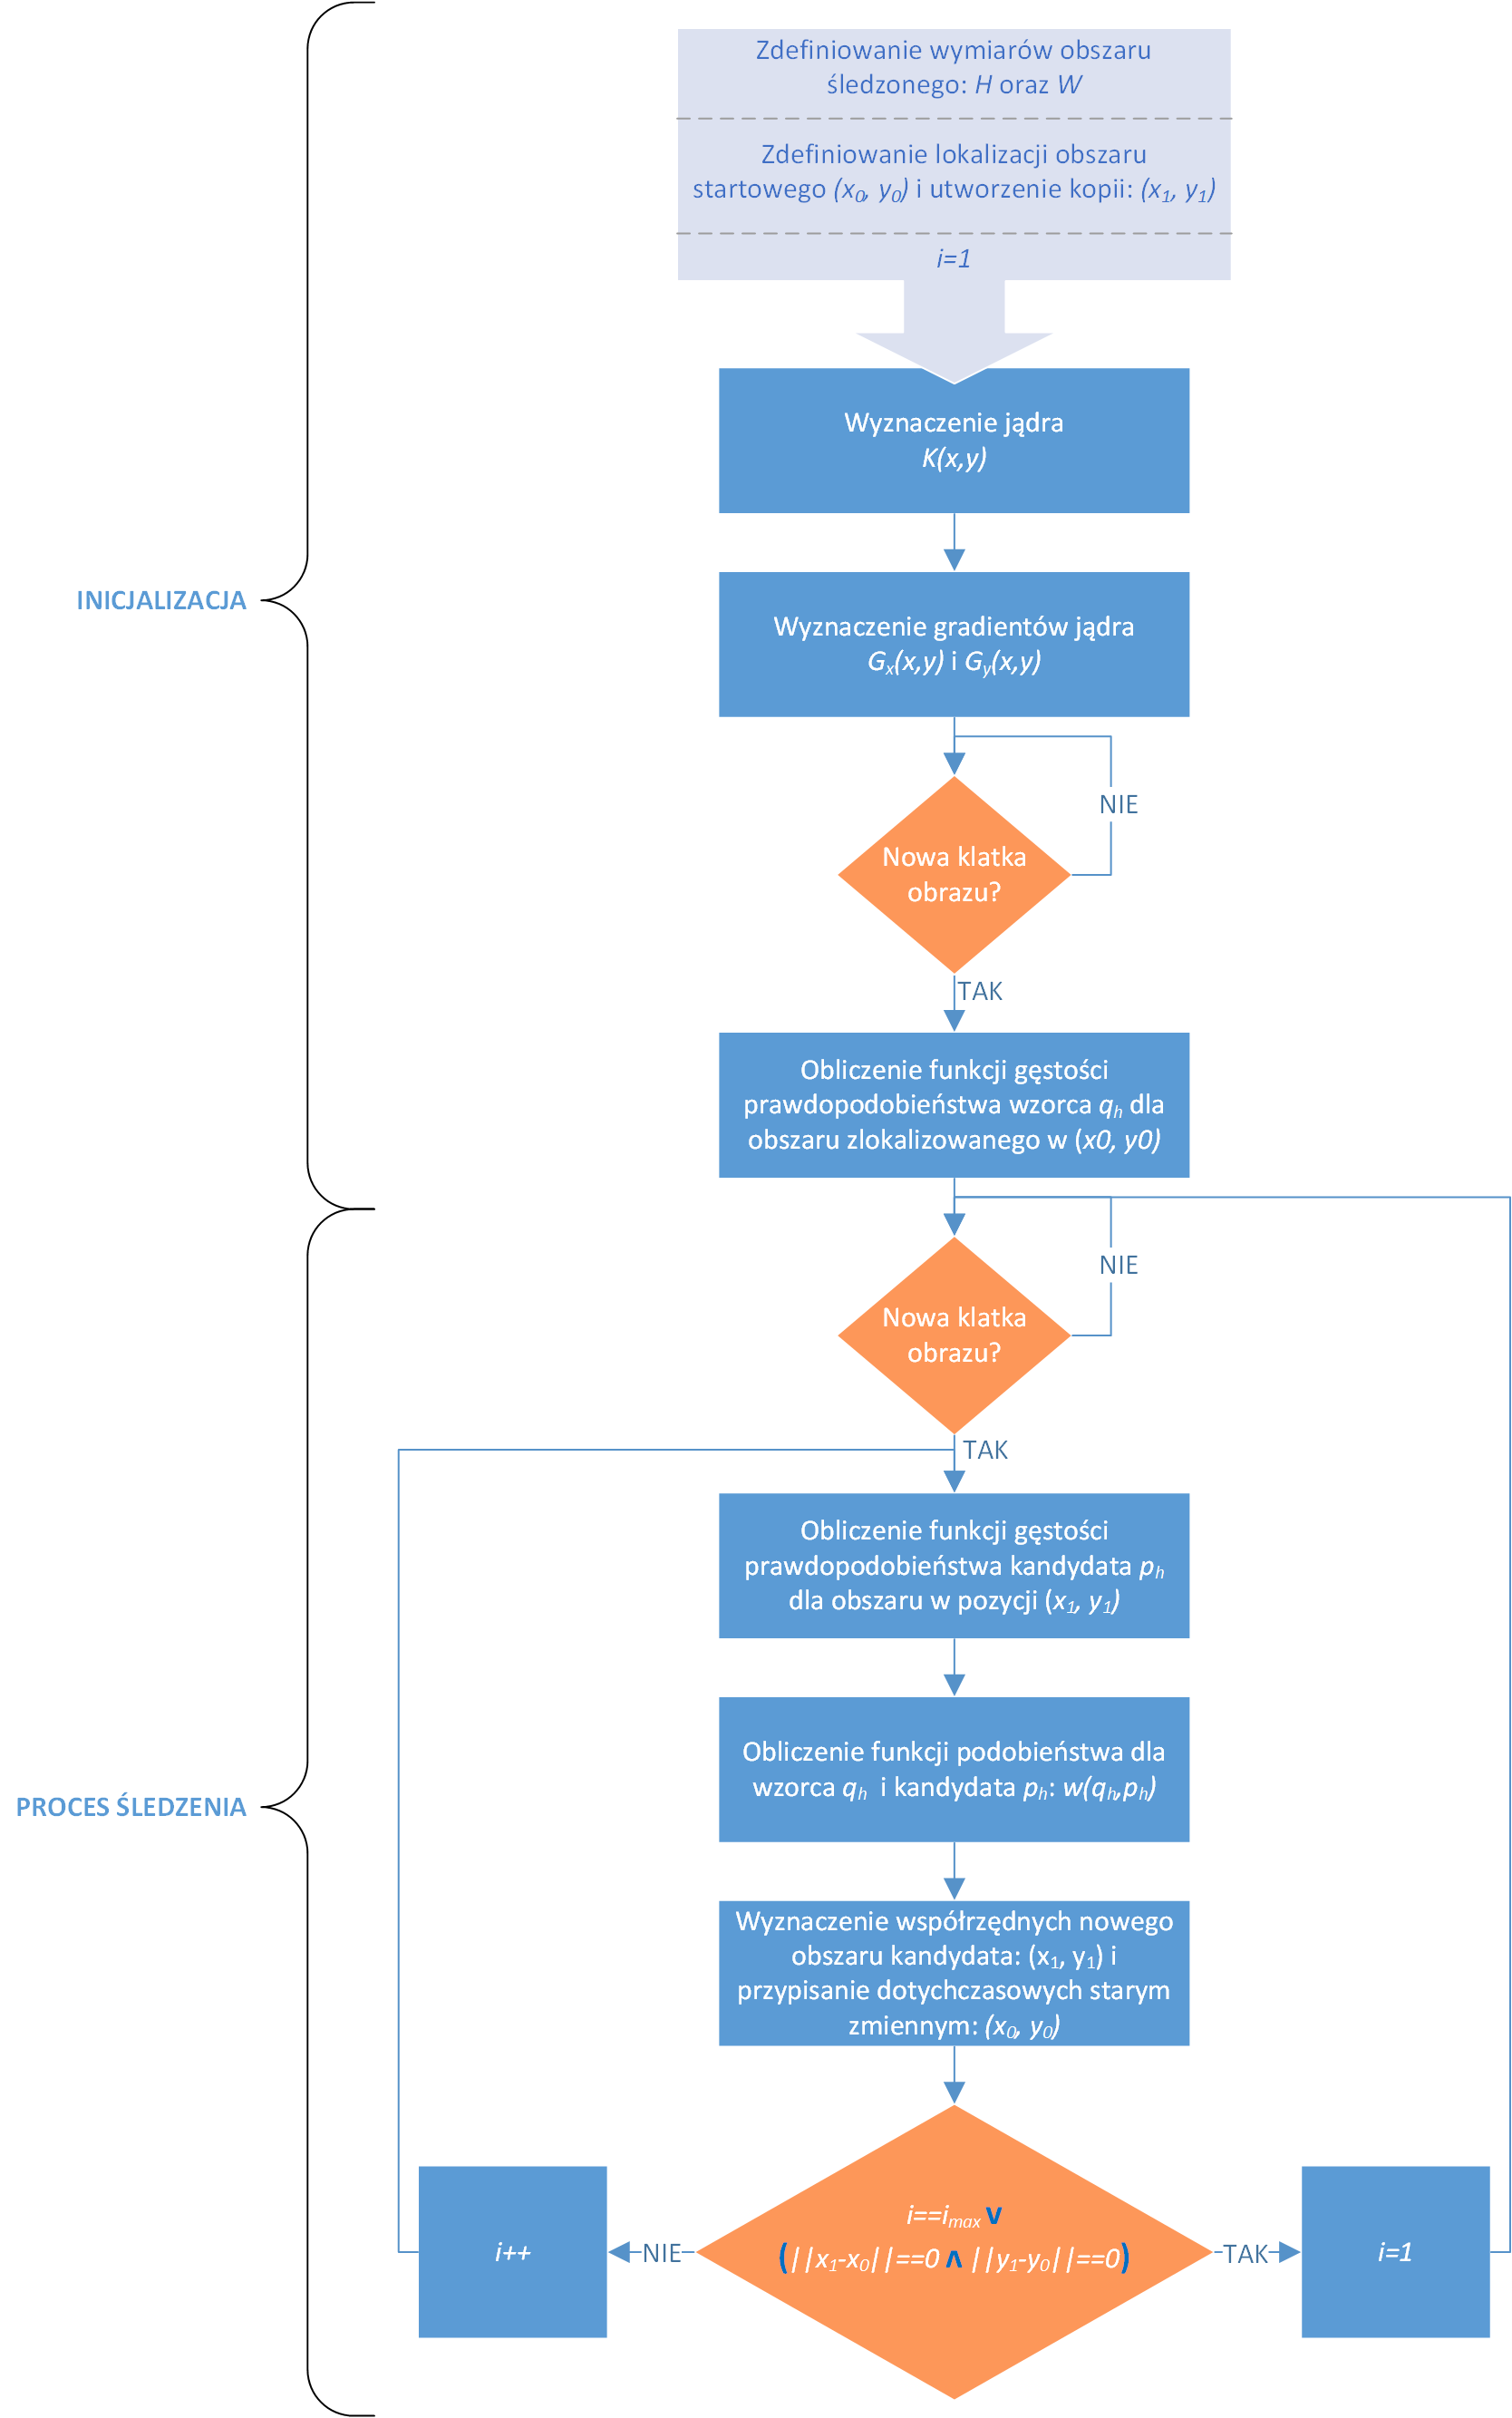
\includegraphics[width=14.5cm]{2_MS_visio.png}
	\caption{Schemat blokowy algorytmu MeanShift}
	\label{fig:MS_scheme}
\end{figure}



\section{Algorytm HOG+SVM}
\label{sec:HOG&SVM}

Jedną z metod śledzenia przez detekcję jest algorytm wykorzystujący zestaw cech obrazu -- konkretnie histogram zorientowanych gradientów (ang. \textit{Histogram of Oriented Gradients - HOG}); rolę decyzyjną pełni klasyfikator nazywany maszyną wektorów nośnych (ang. \textit{Support Vector Machine - SVM}). %TODO śledznie przez detekcję. ukierunk...->zorientowanych %ODP OK
Pierwotnie, rozwiązanie to zostało przedstawione w pracy \cite{Dalal} z zastosowaniem w detekcji pieszych; po nieznacznych zmianach powinno ono osiągnąć dobre wyniki w realizowanym projekcie. %TODO 1. cite, 2 hybrya ? po ,co średni styl. %DOP OK
Metodykę klasyfikacji w oparciu o zestaw cech można również zastosować do detekcji innych obiektów - w szczególności takich, które charakteryzują się dość unikalnym układem krawędzi.
%Oczywiście należy dodać, że dysponując odpowiednim zestawem informacji, odpowiednio trenowany mechanizm SVM byłby w stanie działać z innymi obiektami. %TODO to też takie sobie. Raczej, że podejście można też zastosować do detekcji innych obiektów, w szczególności takich, które charakteryzują się względnie unikalnym układem krawędzi. %ODP OK

Założeniem metody HOG+SVM jest przedstawienie okna detekcji w formie tzw. deskryptora (wektora cech), który pozwoli przeprowadzić proces uczenia klasyfikatora na podstawie dostępnych próbek w sposób umożliwiający skuteczną klasyfikację nowych obrazów. W tym celu okno detekcji dzielone jest na mniejsze, jednakowej wielkości obszary (komórki). Dla każdego z pikseli wewnątrz okna obliczana jest wartość gradientu, jego orientacja i moduł, po czym piksele przydzielone do jednej komórki tworzą histogram zorientowanych gradientów. Okno detekcji jest następnie reorganizowane w formę bloków składających się z współdzielonych pomiędzy sobą 4 komórek (histogramów). Każdy z bloków jest niezależnie normalizowany, po czym wszystkie są łączone w postać wektora cech.\newline
Uczenie maszyny wektorów nośnych polega na wyznaczeniu hiperpłaszczyzny, która rozdzieli deskryptory należące do dwóch klas z maksymalnym marginesem. Klasyfikacja jest etapem prostszym, podczas którego obliczana jest pozycja badanego wektora cech względem hiperpłaszczyzny (określana jest jego klasa).

%TODO Tutaj też jakieś kilka zdań ogólnych i później omówinie konkrentych etapów. %ODP OK

\subsection{Konwersja RGB->GRAY i obliczenie orientacji} %TODO Obliczenie orientacji %ODP OK
\label{sec:HOGgrad}
Pierwszym etapem jest dostosowanie pierwotnej palety barw RGB do 8-bitowej skali szarości. 
Dokonuje się tego, przekształcając każdy piksel według wzoru:
\begin{equation}
\label{eq:rgb2gray}
P_{GRAY}=0.299P_R + 0.587P_G + 0.114P_B 
\end{equation}
%Sumowanie się współczynników do jedności ma w zamierzeniu ograniczyć wynik tego przekształcenia do zakresu 0-255. %TODO zdanie niepotrzebne %ODP OK

%TODO swoją drogę, to w origninalej pracy inaczej jest taktowany obraz RGB, ale niech już będzie. %ODP Michał Drożdż oparł swój algorytm na skali odcieni szarości, wzorowałem się na nim

Następnie przeprowadzana jest operacja kontekstowa w celu obliczenia gradientów kierunkowych $g_x$ oraz $g_y$; używane maski to odpowiednio: $[-1,0,1]$ oraz $[-1,0,1]^T$. 
Mając gradienty, dla każdego piksela (o koordynatach [$i,j$]) obliczany jest moduł i kąt ze wzorów:

\begin{equation}
\label{eq:HOGangles}
\left.\begin{aligned}
m(i,j)=\sqrt{g_x(i,j)^2+g_y(i,j)^2} \\
\theta(i,j)=arctg\bigg(\frac{g_y(i,j)}{g_x(i,j)}\bigg)
\end{aligned}\right.
\end{equation}

\subsection{Histogram gradientów}

W kolejnym etapie poddawany przetwarzaniu obraz jest dzielony na kwadratowe obszary (dla jasności nazywane od teraz \textit{komórkami}) o wymiarach $4\times4$, $8\times8$ lub $16\times16$ pikseli. 
W każdej z komórek zostanie wyliczony niezależny histogram na podstawie orientacji gradientu. %TODO kątów -> orientacji %ODP OK
Oprócz rozmiaru komórki, kluczowym okazuje się również drugi parametr, czyli liczba przedziałów pojedynczego histogramu -- w tym wypadku zdecydowano, by rozpatrywany kąt przyporządkowywać jednemu z 9 przedziałów określających kierunek (z pominięciem zwrotu). Dzielą one równo zakres kątów $[0^{\circ},180^{\circ})$ -- i odpowiednio $[-180^{\circ},0^{\circ})$. %TODO przedziałów klasowych ??, komplementarnie - nie wynika z tego, że "zwrot" jest pomijane] %ODP OK
Wynika z tego, że każdy kolejny fragment o szerokości $a=180^{\circ}/9=20^{\circ}$ będzie stanowić osobny przedział histogramu. %TODO jw. %ODP OK

O ile typowy histogram tworzony jest poprzez inkrementację odpowiedniego licznika dla przedziału o 1, to tworzona struktura będzie wykorzystywać obliczony wcześniej moduł z gradientu. 
Dodatkowo, autorzy publikacji wspominają o możliwości interpolacji pomiędzy dwoma sąsiednimi przedziałami i inkrementacji poszczególnych wartości o proporcjonalne części modułu -- dowiedziono eksperymentalnie, że takie działanie pozytywnie wpływa na wyniki detekcji. %TODO nie ma tylko wypływa - są na dowody w tej pracy (eksperymentalne) %ODP OK
Jeśli zatem przyjąć, że $\theta_h$ i $\theta_l$ to wartości kątów będących środkami dwóch sąsiadujących ze sobą przedziałów, którym jednocześnie najbliżej do badanego kąta $\theta$, wówczas będzie można zdefiniować elementy $M_h$ i $M_l$ jako: %TODO inkrementy ??? %ODP OK

\begin{equation}
\label{eq:HOG_linear}
\left.\begin{aligned}
M_h(i,j)&=m(i,j)\bigg(\frac{\theta-\theta_l}{a}\bigg)\\
M_l(i,j)&=m(i,j)\bigg(\frac{\theta_h-\theta}{a}\bigg)
\end{aligned}\right.
\end{equation}

Ostatecznie, następuje powiększenie wartości dwóch odpowiednich przedziałów histogramu $H$ tworzonego w obrębie komórki zawierającej piksel o współrzędnych (i,j):

\begin{equation}
\label{eq:HOG_increment}
\left.\begin{aligned} 
H(\theta_h,i,j)&=H(\theta_h)+M_h(i,j) \\ 
H(\theta_l,i,j)&=H(\theta_l)+M_l(i,j)
\end{aligned}\right.
\end{equation}

Koncepcję zilustrowano na rysunku \ref{fig:HOG_interpolation}.  %TODO Koncepcję zilutrowano na rysunku XXX %ODP OK
Przedstawia on okrąg z ponumerowanymi przedziałami, każdy o szerokości $a$. Jeśli orientacja obliczonego gradientu jest reprezentowana przez kąt $\theta=57^{\circ}$, to przedziałami uwzględnionymi w interpolacji będą te najbliższe, o numerach $3$ oraz $4$. Bazując na wartości kątów w ich środkach, $\theta_h$ i $\theta_l$, obliczane zostaną $M_h$ i $M_l$, jako odpowiednio: $35\%$ i $65\%$ wartości modułu zgodnie z wzorami \eqref{eq:HOG_linear}.
%TODO Lepiej opisać ten rysunek ! %ODP OK
Wyjątkowym zdarzeniem jest takie, w którym kąt $\theta$ będzie znajdował w okolicy kąta $0^{\circ}=360^{\circ}$ (z przedziałami 1 oraz 9). 
Wówczas, dla wygody, w równaniach \eqref{eq:HOG_linear} należy użyć kątów $\theta_l=350^{\circ}$ oraz $\theta_h=370^{\circ}$.

\begin{figure}[h]
	\centering
	\hspace*{1cm}
	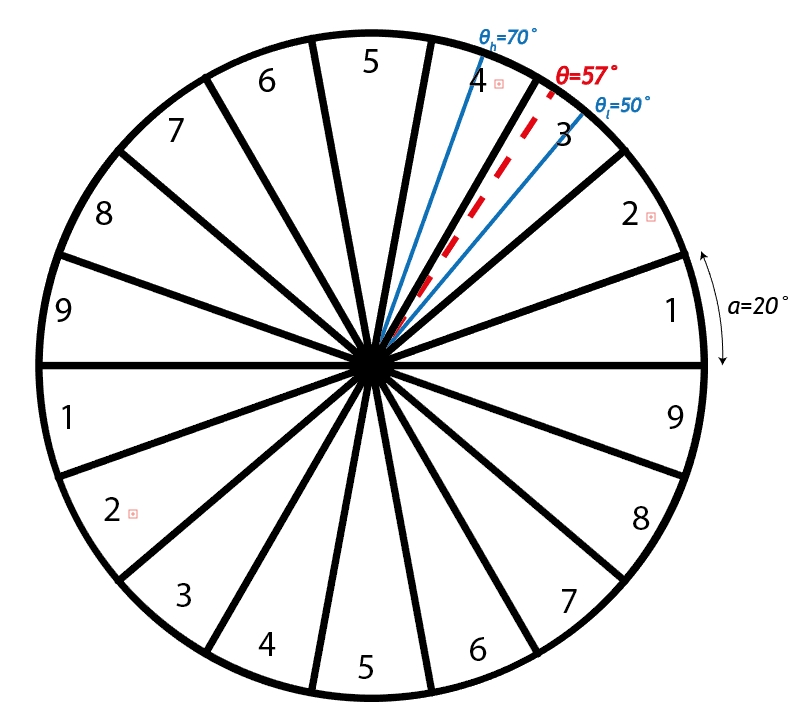
\includegraphics[width=12cm]{2_HOG_interpolation.jpg}
	\caption{Przykładowy problem liniowej interpolacji}
	\label{fig:HOG_interpolation}
\end{figure}

\subsection{Normalizacja}

Zazwyczaj, analizowany materiał wideo będzie rejestrowany w warunkach, w których ciężko zagwarantować równy poziom oświetlenia poszczególnych fragmentów obrazu. %TODO nie amatroskich... w warunkach, w których ciężko zagwarantować... %ODP OK
Zakłócenia te negatywnie wpływają na wyniki działania algorytmu.
%Zdegenerowany w ten sposób obraz nie dawałby dobrych wyników działania algorytmu.  
%TODO Zakłócenie te nagatywnie... %ODP OK
Z tego powodu proponuje się stosowanie blokowej normalizacji. 

Proponowane podejście zakłada utworzenie struktur nazywanych \textit{blokami}, gdzie każdy z nich obejmować ma $2\times 2$ sąsiednie komórki. 
Dla obrazu, na bazie którego utworzono $N \times M$ komórek, powinno powstać $N-1 \times M-1$ bloków -- przy ich generowaniu wykonuje się krok o jedną komórkę w poziomie i/lub w pionie względem poprzedniego obszaru. 
Rozmiar pojedynczego bloku sugeruje, że będzie się on składał z 4 histogramów, w formie wektora: 
\begin{equation}
v=[H_{i,j}, H_{i,j+1}, H_{i+1,j}, H_{i+1,j+1}],
\end{equation} 
gdzie: $i$  wiersz, $j$ - kolumna. Następnie należy dokonać normalizacji, wykorzystując jedną z sugerowanych zależności: %TODO raczej dokonać normalizacji.. %ODP OK

\begin{equation}
\label{eq:HOG_norm1}
\left.\begin{aligned} 
L1&=\frac{v}{\sum_{i}^{n}v_i+\epsilon}
\end{aligned}\right.
\end{equation}

\begin{equation}
\label{eq:HOG_norm2}
\left.\begin{aligned} 
L1_{sqrt}&=\frac{v}{\sqrt{\sum_{i}^{n}v_i+\epsilon}}
\end{aligned}\right.
\end{equation}

\begin{equation}
\label{eq:HOG_norm3}
\left.\begin{aligned} 
L2&=\frac{v}{\sqrt{\sum_{i}^{n}v_i^2+\epsilon^2}}
\end{aligned}\right.
\end{equation}

\begin{equation}
\label{eq:HOG_norm4}
\left.\begin{aligned} 
L2_{hys}&=\frac{v}{\sqrt{\sum_{i}^{n}v_i^2+\epsilon^2}}, v\leq 0.2
\end{aligned}\right.
\end{equation}
W powyższych równaniach $\epsilon$ to stała o małej wartości, a $n$ to liczba elementów w bloku (4 histogramy po 9 przedziałów $\rightarrow$ 36). Wektory $L$ zebrane z całego okna detekcji budują ostateczny wektor cech, na którym pracować będzie klasyfikator.

Niech podsumowaniem rozważania będzie przykład -- okno detekcji o rozmiarze $200\times 400$ i komórka o wielkości $8 \times 8$. 
Wynikiem opisywanej procedury będzie utworzenie aż $25\cdot50=1250$ komórek i $24\cdot 49=1176$ bloków. 
Po normalizacji, klasyfikator otrzymałby aż $1176\cdot4\cdot9=42336$ wartości do przetworzenia. 
Obsługa tak dużej ilości danych niesie za sobą konieczność pewnych optymalizacji, co będzie rozważone w rozdziale poświęconym implementacji algorytmu.
%TODO przykłąd nietafiony, bo zawsze się wykonuje detekcję w oknach %ODP wielkość zmieniono, chodziło mi raczej o przejście przez obliczenia na jakimkolwiek przykładzie.

\subsection{Klasyfikator SVM}

Maszyna wektorów nośnych to klasyfikator binarny, który dzięki swej prostocie i skuteczności jest powszechnie wykorzystywany w procesie odróżniania klas w różnych aplikacjach, w tym wizyjnch \cite{Gunn}. %TODO w różnych aplikacjach, w tym wizyjnch. %ODP OK
Jego działanie tradycyjnie można podzielić na dwie fazy: uczenie i klasyfikację. 
Etap uczenia to relatywnie dłuższy czasowo proces wyznaczenia hiperpłaszczyzny, która z jak najlepszym marginesem rozdzieli wejściowe wektory cech obiektów klasyfikowanych jako \textit{1} od tych określonych jako \textit{0} (umownie). 
Stosowane podeście nie powinno odbiegać od klasycznej metodologii uczenia maszynowego -- dysponując zbiorem danych wejściowych, należy dokonać podziału na próbki uczące oraz testowe (w stosunku około 70:30). %TODO trenujące -> uczące %ODP OK
Każdy z tych podzbiorów (a przede wszystkim uczący) powinien posiadać zarówno obiekty zdefiniowane jako pozytywne, jak i negatywne. 
W niniejszej pracy, która ma na celu rozpoznanie osoby w postawie stojącej, wymagane będzie użycie obrazów o rozmiarch $128\times64$, przedstawiających taką postać w jak największej liczbie kombinacji (ale w podobnej skali), lecz także obrazów ze zróżnicowaną scenerią, na których żadnych osób jednak nie ma. 
%TODO z tym wyraźnie odmiennym to byłbym ostrożny  ... %ODP OK
Dla poprawienia ostatecznych wyników należy zadbać również o zróżnicowanie obrazów pod kątem poziomu oświetlenia, a nawet tła otaczającego postać.
Etapem klasyfikacji nazwać można wykorzystanie otrzymanych w procesie uczenia parametrów do wyznaczenia położenia badanego wektora cech względem hiperpłaszczyzny. 
Na tej podstawie do obiektu zostanie przydzielona odpowiednia klasa.

%TODO przydałoby się równianie SVM z opisem. %ODP niżej

\subsubsection{Uczenie}

Aby detektor mógł działać poprawnie, klasyfikator musi dysponować odpowiednimi parametrami. 
Uzyskuje się je na etapie uczenia, używając odpowiedniego zestawu danych.
Wzorując się na pracy Dalala oraz Triggsa, postanowiono skorzystać ze zbioru ponad 5000 obrazów udostępnionych przez twórców. 
Specyfikacja tego zestawu pozwala nauczyć klasyfikator rozpoznawania osoby na obrazie o wielkości $128\times 64$ pikseli. 
Wysokość przedstawionej osoby, wyrażona w pikselach, powinna oscylować wokół 95 ($\pm$ 5). 
Zgodnie z przyjętymi metodologiami, zestaw ten zawiera gotowy podział na próbki pozytywne i negatywne, dalej pogrupowane na zestaw uczący oraz testowy w stosunku zbliżonym do 70:30. %TODO uczący/testowy %ODP OK
Przykłady przedstawiono na ilustracji:

\begin{figure}[h]
	\centering
	\captionsetup{justification=centering,margin=1cm}
	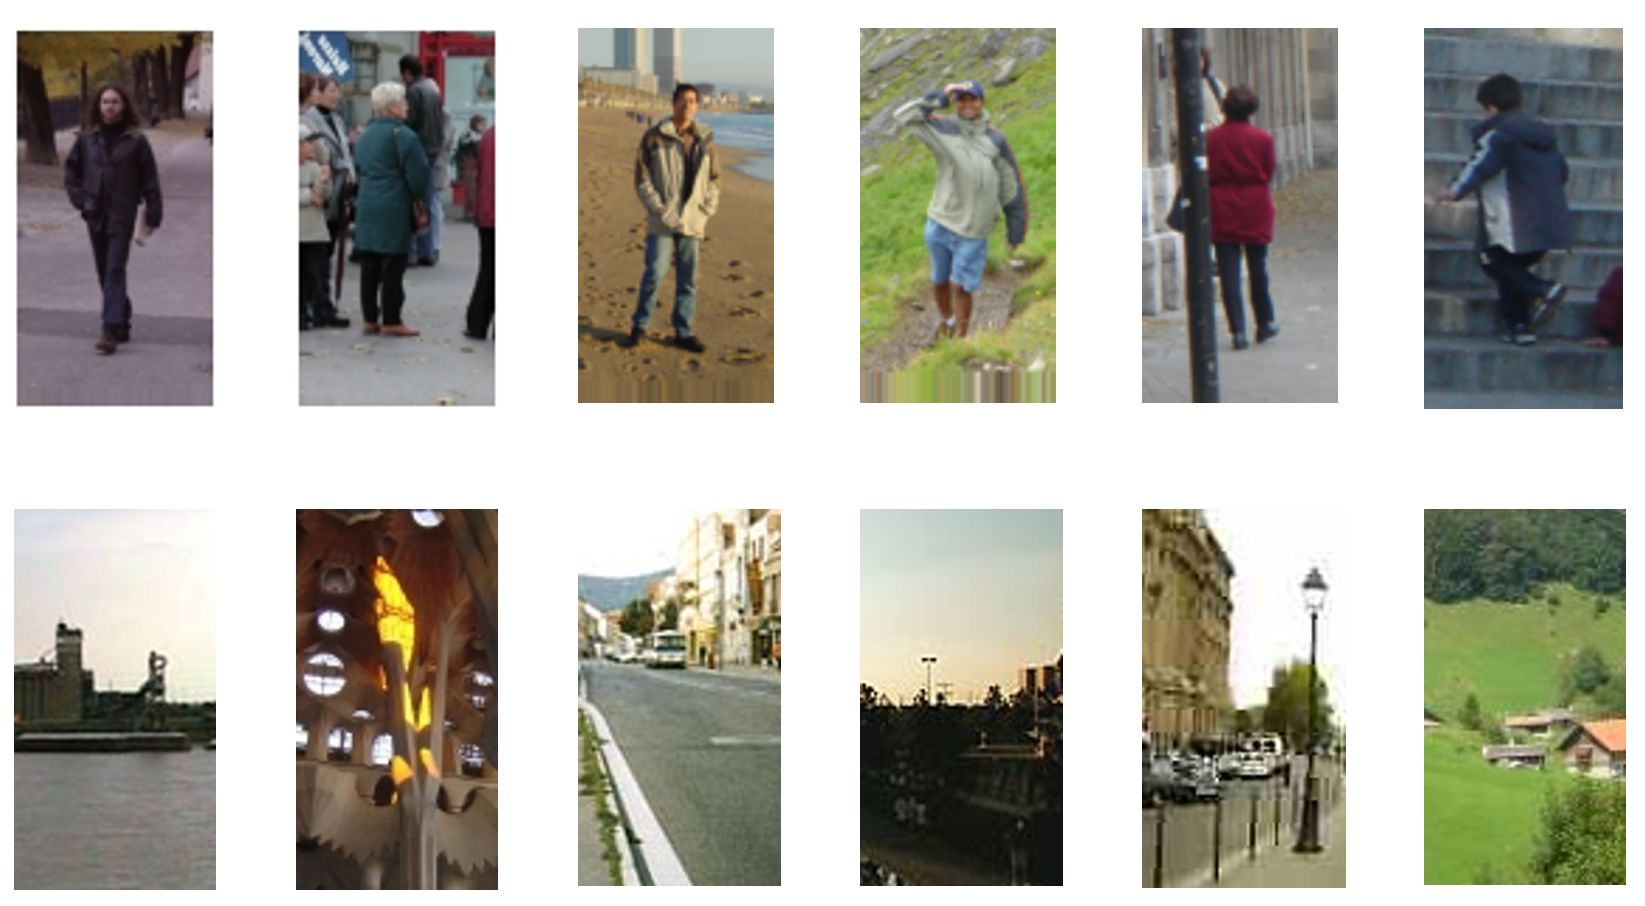
\includegraphics[width=14.5cm]{2_HOG_image_examples.jpg}
	\caption{Przykłady obrazów ze zbioru wykorzystanego przy uczeniu -- na górze próbki pozytywne, na dole negatywne}
	\label{fig:HOG_image_examples}
\end{figure}
%TODO no ale dlaczego te megatywne mają inne rozmiary ? powinny mieć przecież takie same. I może wiecej przykładów. %ODP rozmiary były inne w bazie INRIA - ale do uczenia/testów wykorzystywało się i tak wycinki 128x64. Dodano więcej przykładów
Wśród próbek pozytywnych połowa plików to duplikaty odwrócone horyzontalnie. Ma to zapewnić poprawne uwzględnienie cech osób niezależnie od orientacji względem kamery.

\subsubsection{Klasyfikacja}
\label{sec:klasyfikacja}
Etap ten jest stosunkowo prosty i stanowi główną zaletę klasyfikatora SVM. 
Wymaga bowiem wcześniejszego przeprowadzenia etapu uczenia oraz dostarczenia wektora cech klasyfikowanego obiektu. 
Realizowane jest wówczas równanie:
\begin{equation}
\label{eq:HOG_classification}
\left.\begin{aligned} 
r=\sum_{i=1}^{N}(a_i\cdot l_i)+b,
\end{aligned}\right.
\end{equation}
gdzie $l_i$ to elementy wektora cech, natomiast $a_i$ i $b$ to parametry wyliczone na etapie uczenia. 

W projekcie, proces uczenia i klasyfikacji oparto o funkcje dostępne w środowisku MATLAB, gdzie to równanie jest nieco zmodyfikowane:
\begin{equation}
\label{eq:HOG_classificationMATLAB}
\left.\begin{aligned} 
r=-\sum_{i=1}^{N}a_i(l_i+b_i)-c,
\end{aligned}\right.
\end{equation}
gdzie $a$, $b$ oraz $c$ to parametry hiperpłaszczyzny wyliczone na etapie uczenia ($a$ i $b$ - wektory, $c$ - skalar).

Dla obu przypadków, detekcja wskazuje obiekt jako przynależący klasy jeśli $r>0$, w przeciwnym wypadku go odrzuca.
%TODO nie podoba mi się a postać równania. Zykle jest inna. suma wagi x wektor cech +b > 0 %ODP opisano nieco więcej na ten temat

\subsection{Detekcja na ramce obrazu}
%TODO Wcześniej trzeba zaznaczyć, że rozważania dotyczą klasyfikacji próbek z sylwektami/lub bez o rozmiarch np to 128 x 64. %ODP OK
%TODO A ten rozdział to detekcja na ramce obrazu. %ODP OK

Klasyfikator jest w stanie rozpoznać postać znajdującą się w centrum próbki o rozmiarze $128\times 64$. 
%TODO druga część zdania niejasne %ODP OK, określono w pierwszej części zdania

Osiągnięcie dobrych wyników detekcji wymaga zastosowania mechanizmu okna przesuwnego. Dysponując określonym obszarem zainteresowań, algorytm powinien sprawdzić każdą możliwą konfigurację położenia okna $128\times 64$ wewnątrz tego obszaru. Oznaczać to przesuwanie okna o 1 piksel w bok, a po dotarciu do prawej linii o 1 piksel w dół. Takie podejście skutkuje bardzo dużą złożonością obliczeniową - dla obszaru zainteresowań o wymiarach $144\times 96$ i rozpatrywanego okna istnieje 512 możliwości (512 wektorów cech). W praktyce zwiększa się wykonywany krok o kilka lub kilkanaście pikseli.

Metoda HOG+SVM jest mało odporna na zmianę wielkości wykrywanego obiektu na oryginalnym obrazie, a porównując wymiary ramki ($1280\times 720$) z wielkością okna detekcji, może wydawać się to poważnym ograniczeniem. Skutecznym rozwiązaniem okazuje się być zastosowanie algorytmu HOG+SVM na kilku przeskalowanych w różny sposób kopiach obrazu. Z każdej skali należy wydobyć próbki obrazów o wymiarach $128\times 64$ i znaleźć najlepszą pozytywną detekcję. Odpowiadająca wybranemu wynikowi skala da również pośrednią informację o odległości. 

Metodyka detekcji w wielu skala stanowi dobrą odpowiedź na jedno z założeń systemu, mówiące o konieczności określenia odległości kamery od rozpoznanej osoby, by poprzez odpowiednie sterowanie utrzymać zadany dystans.  %TODO z tym kierunkiem ? -> niejasne %ODP OK

Opisują to rysunki \ref{fig:HOG_scaling}. %TODO Ilustrują i nie poniżej tylko \ref %ODP OK
\begin{figure}[h]
	\centering
	\captionsetup{justification=centering,margin=1cm}
	\hspace*{0cm}
	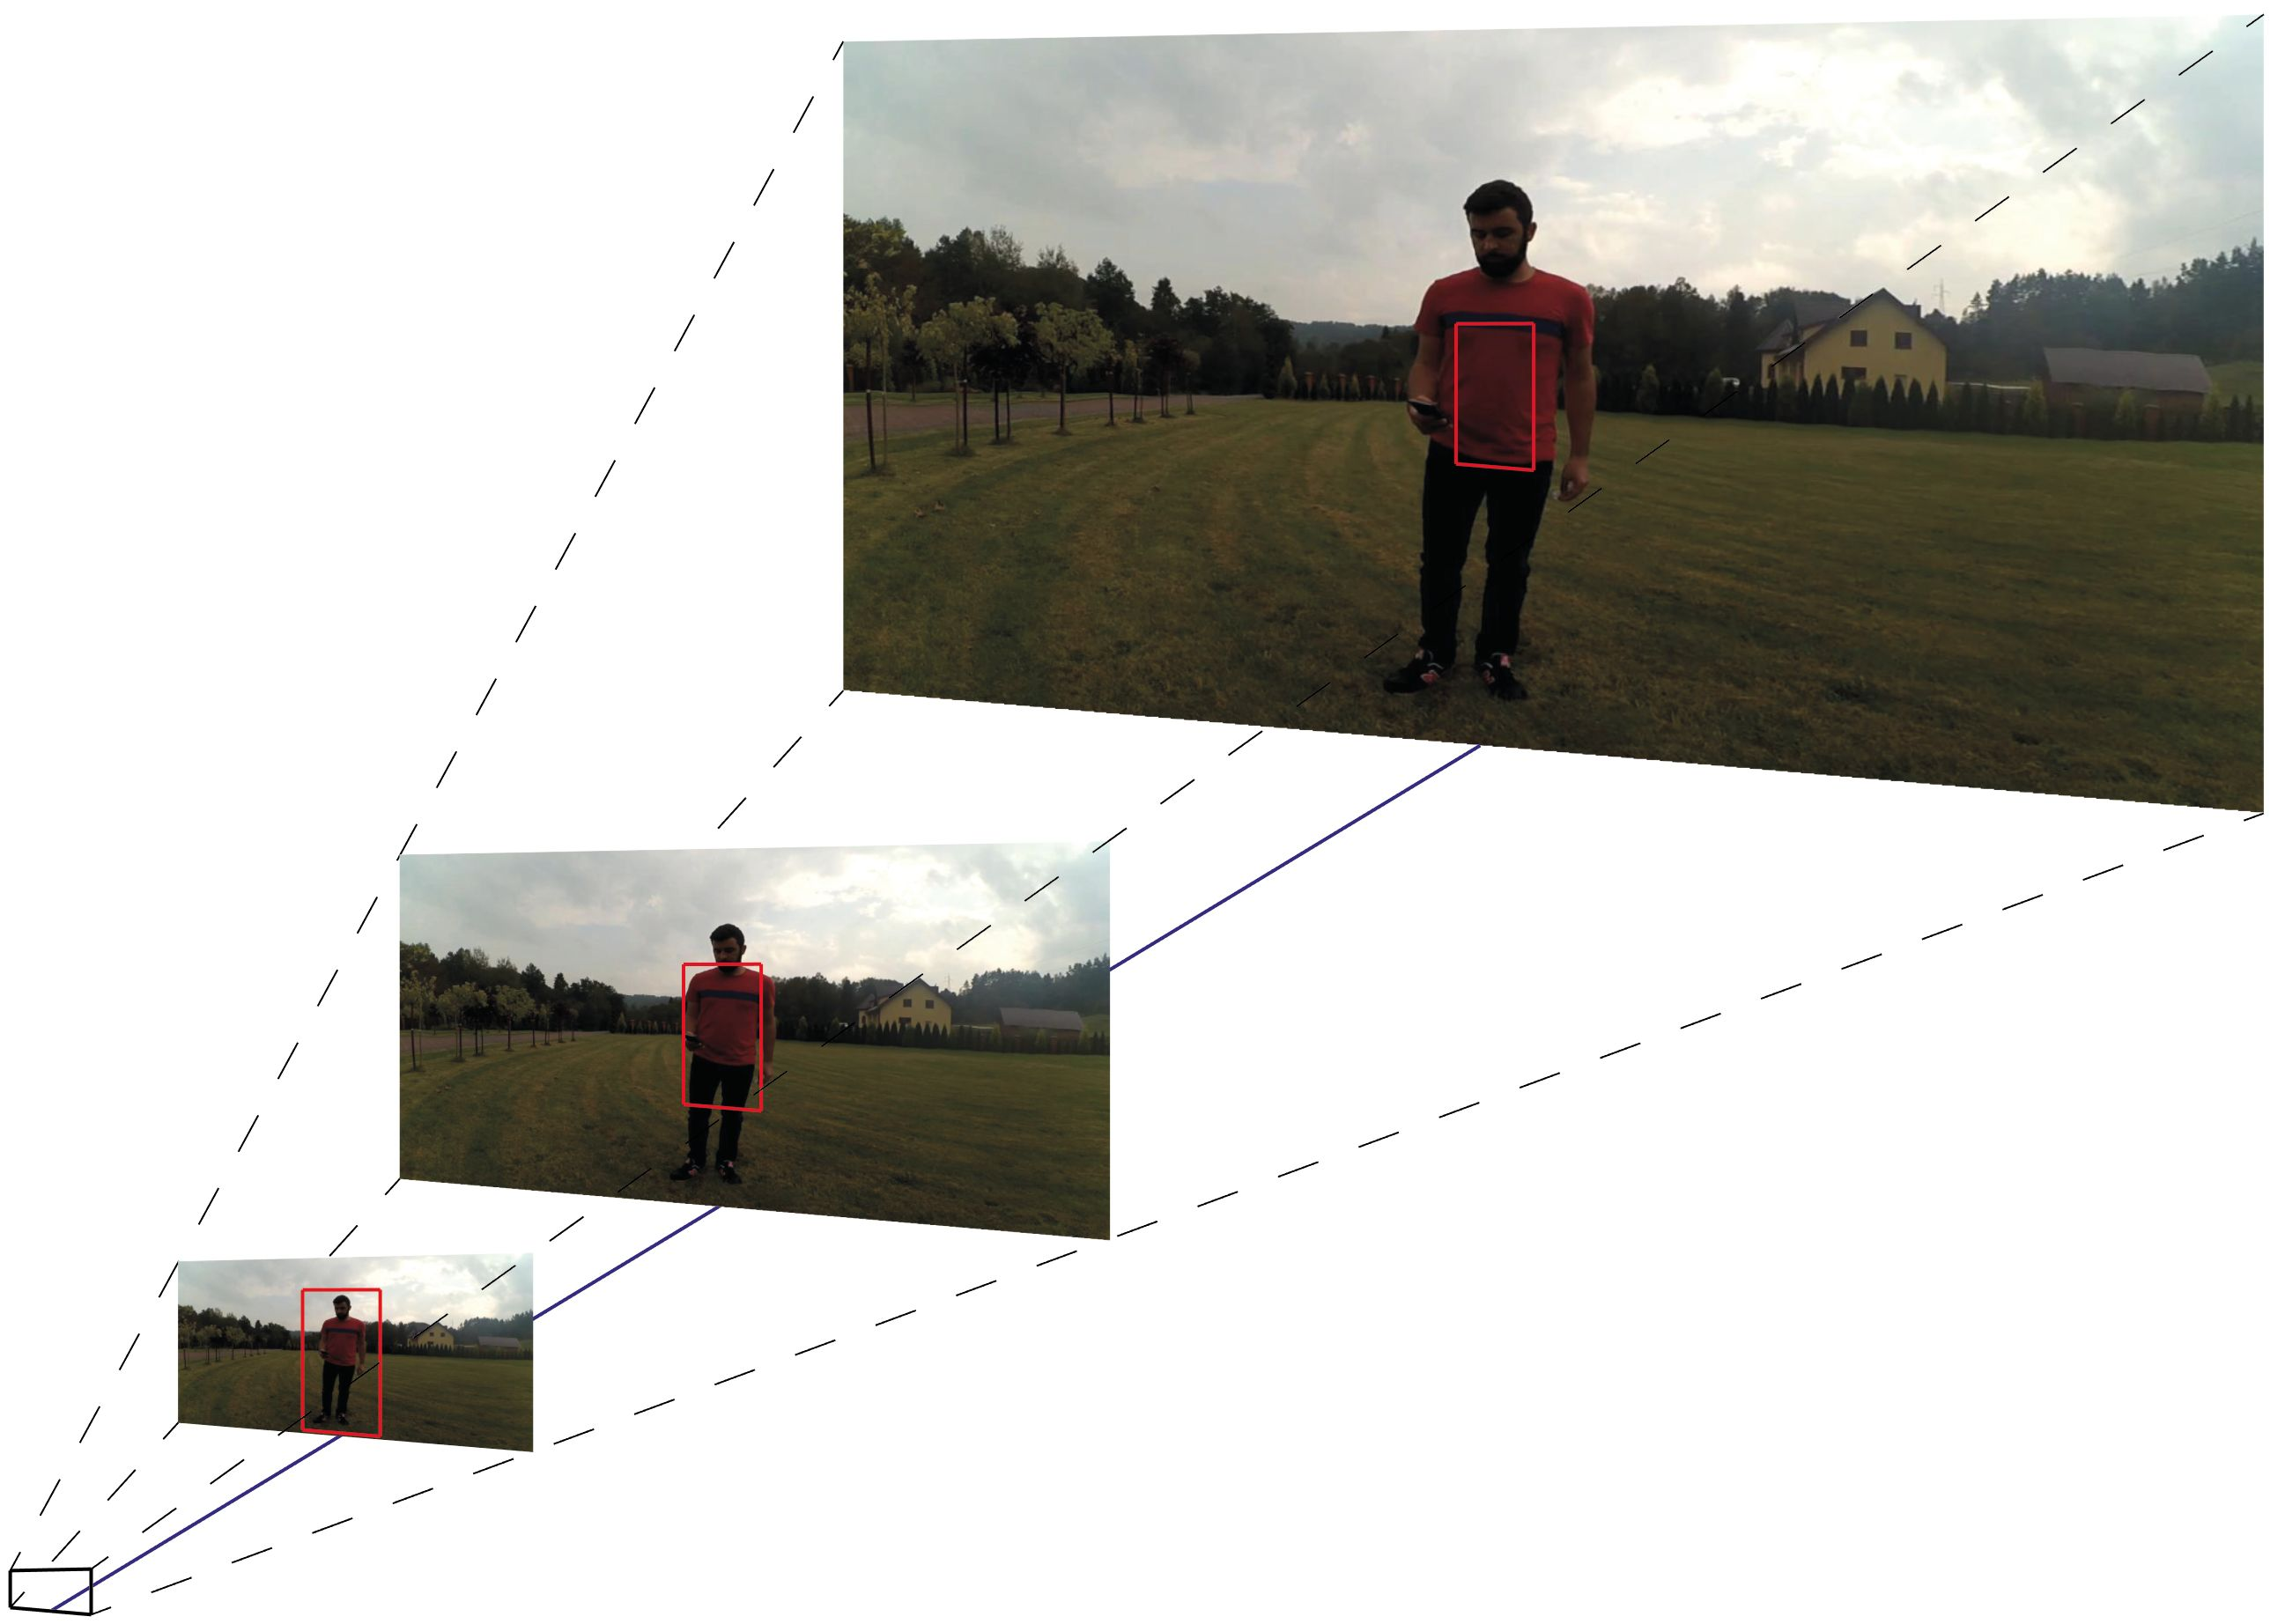
\includegraphics[width=15.5cm]{2_scaling.jpg}
	\caption{Skalowanie 1:1, 1:2 oraz 1:4 z naniesionym przykładowym oknem detekcji $128 \times 64$}
	\label{fig:HOG_scaling}
\end{figure}
\newline

Stała wielkość okna detekcji każe wnioskować, że osoba wykryta na oryginalnym obrazie byłaby znacząco oddalona od kamery. W przypadku przedstawionym na rysunku, klasyfikator prawdopodobnie rozpozna postać na oknie detekcji z obrazu przeskalowanego w stosunku 1:4. %TODO styl. to nie okno rozpoznaje... %ODP OK
Znając przybliżoną odległość pomiędzy kamerą oraz osobą wykrywaną przez takie okno na oryginalnym obrazie i stosując proste twierdzenie Talesa, można oszacować jej rzeczywistą odległość dla pozytywnej detekcji w jednej ze skal. Opisuje to poniższy wzór:
\begin{equation}
\label{eq:scaling}
d_r=\frac{d_o}{s_c},
\end{equation}
gdzie $d_r$ to aktualna odległość pomiędzy osobą i kamerą , $d_o$ to odległość do wykrytej osoby na obrazie oryginalnym (zmierzona), a $s_c$ to skala obrazu (w postaci ułamkowej), w którym okno detekcji uzyskało najlepszy wynik.

%TODO co jest rozumiene przez odległość ? %ODP wyjaśniono



%TODO tu komplemetnie brakuje  opisu jak działa tzw. okno przesuwne.  Same skale też można lepiej opisać. %ODP Dodano opis, w rozdziale o implementacji jest o tym więcej napisane
%TODO Kolejna sprawa to tzw. grupowienie detekcji z wielu skal. %ODP to mam opisane w implementacji 

%TODO rozdziały o klasyfikacji i uczeniu połączyć z SVM, a to przetwarzanie dla cłąej ramk na końcu. %ODP OK


\chapter{Implementacja modelu programowego}
%TODO Jak już opisze Pan na początku koncpecję to będzie to jasne. Tu trzeba się do tego odwołać. Bo w tej postaci to to wygląda tak, że sobie Pan to po prostu rozaważa... %ODP OK

Pierwszym etapem weryfikującym poprawność przedstawionej koncepcji było stworzenie modeli programowych algorytmów MeanShift oraz Hog+SVM, bez warstwy nadzorującej/sterującej dronem. 
Wybrano środowisko MATLAB ze względu na jego powszechne zastosowanie w branży naukowej/inżynierskiej, co skutkuje olbrzymią bazą bibliotek i materiałów pomocniczych. 
W tym przypadku MATLAB ułatwia pracę na obrazach lub sekwencjach wideo poprzez: wczytywanie materiału, wyświetlanie, dostęp do poszczególnych klatek oraz zapewnia wiele wbudowanych funkcji, m.in. do konwersji określonych przestrzeni barw oraz klasyfikacji z wykorzystaniem maszyny wektorów nośnych. %TODO może klasyfikacji z wykorzystaniem %ODP OK

\section{Model MeanShift}

Skrypt rozpoczyna działanie od wyznaczenia jądra obszaru o wymiarach $100 \times 100$ (zgodnie ze schematem \ref{fig:kernel_build}) oraz jego gradientów. %TODO tu by się przydały odnośniki do stosowanych wzorów.
Po tym następuje właściwa część algorytmu, która pracuje na wczytanym materiale wideo, przekonwertowanym do przestrzeni HSV. 
Obszarem śledzonym jest kwadrat $100\times 100$, który dla pierwszej klatki obrazu jest zlokalizowany w miejscu obecności śledzonego obiektu. %TODO co to jest miejsce startowe ??? %ODP OK
Dla tego fragmentu obliczany jest histogram barw. 
Następnie, dla kolejnych klatek, obliczany jest histogram kandydatów ostatecznie zestawiając go z oryginalnym i wyznaczając przesunięcie w pionie i poziomie. %TODO styl. Następnie, dla kolenych klatek, obliczane.... %ODP OK
Dla każdej z klatek operacja ta jest przeprowadzana 10 razy, poprawiając precyzję ostatecznego przesunięcia. 
Przed rozpoczęciem przetwarzania kolejnej klatki, następuje aktualizacja pozycji śledzonego obszaru. %TODO Obszaru ? %ODP OK
Po wykonaniu algorytmu dla zdefiniowanej liczbie klatek, skrypt wyświetla film w oryginalnych barwach RGB z dorysowaną czerwoną ramką otaczającą śledzony obszar, co pozwala wizualnie sprawdzić poprawność działania całego kodu. 
Niestety, czas wykonania tej symulacji jest nieporównywalnie dłuższy od rzeczywistego trwania sekwencji i, przykładowo, na komputerze wyposażonym w procesor klasy i7 materiał o długości 685 klatek (ok. 11 sekund filmu) jest przetwarzany w czasie ok. 100 sekund.

Rysunek \ref{fig:meanshift_prog} przedstawia śledzenie obiektu w postaci czerwonej koszulki z ciemnym poziomym paskiem. Kolejne zrzuty są realizowane z odstępem 100 klatek. Zauważyć można poprawne działanie algorytmu nawet pomimo zmiany odległości obiektu od kamery.
 
\begin{figure}[]
	\centering
	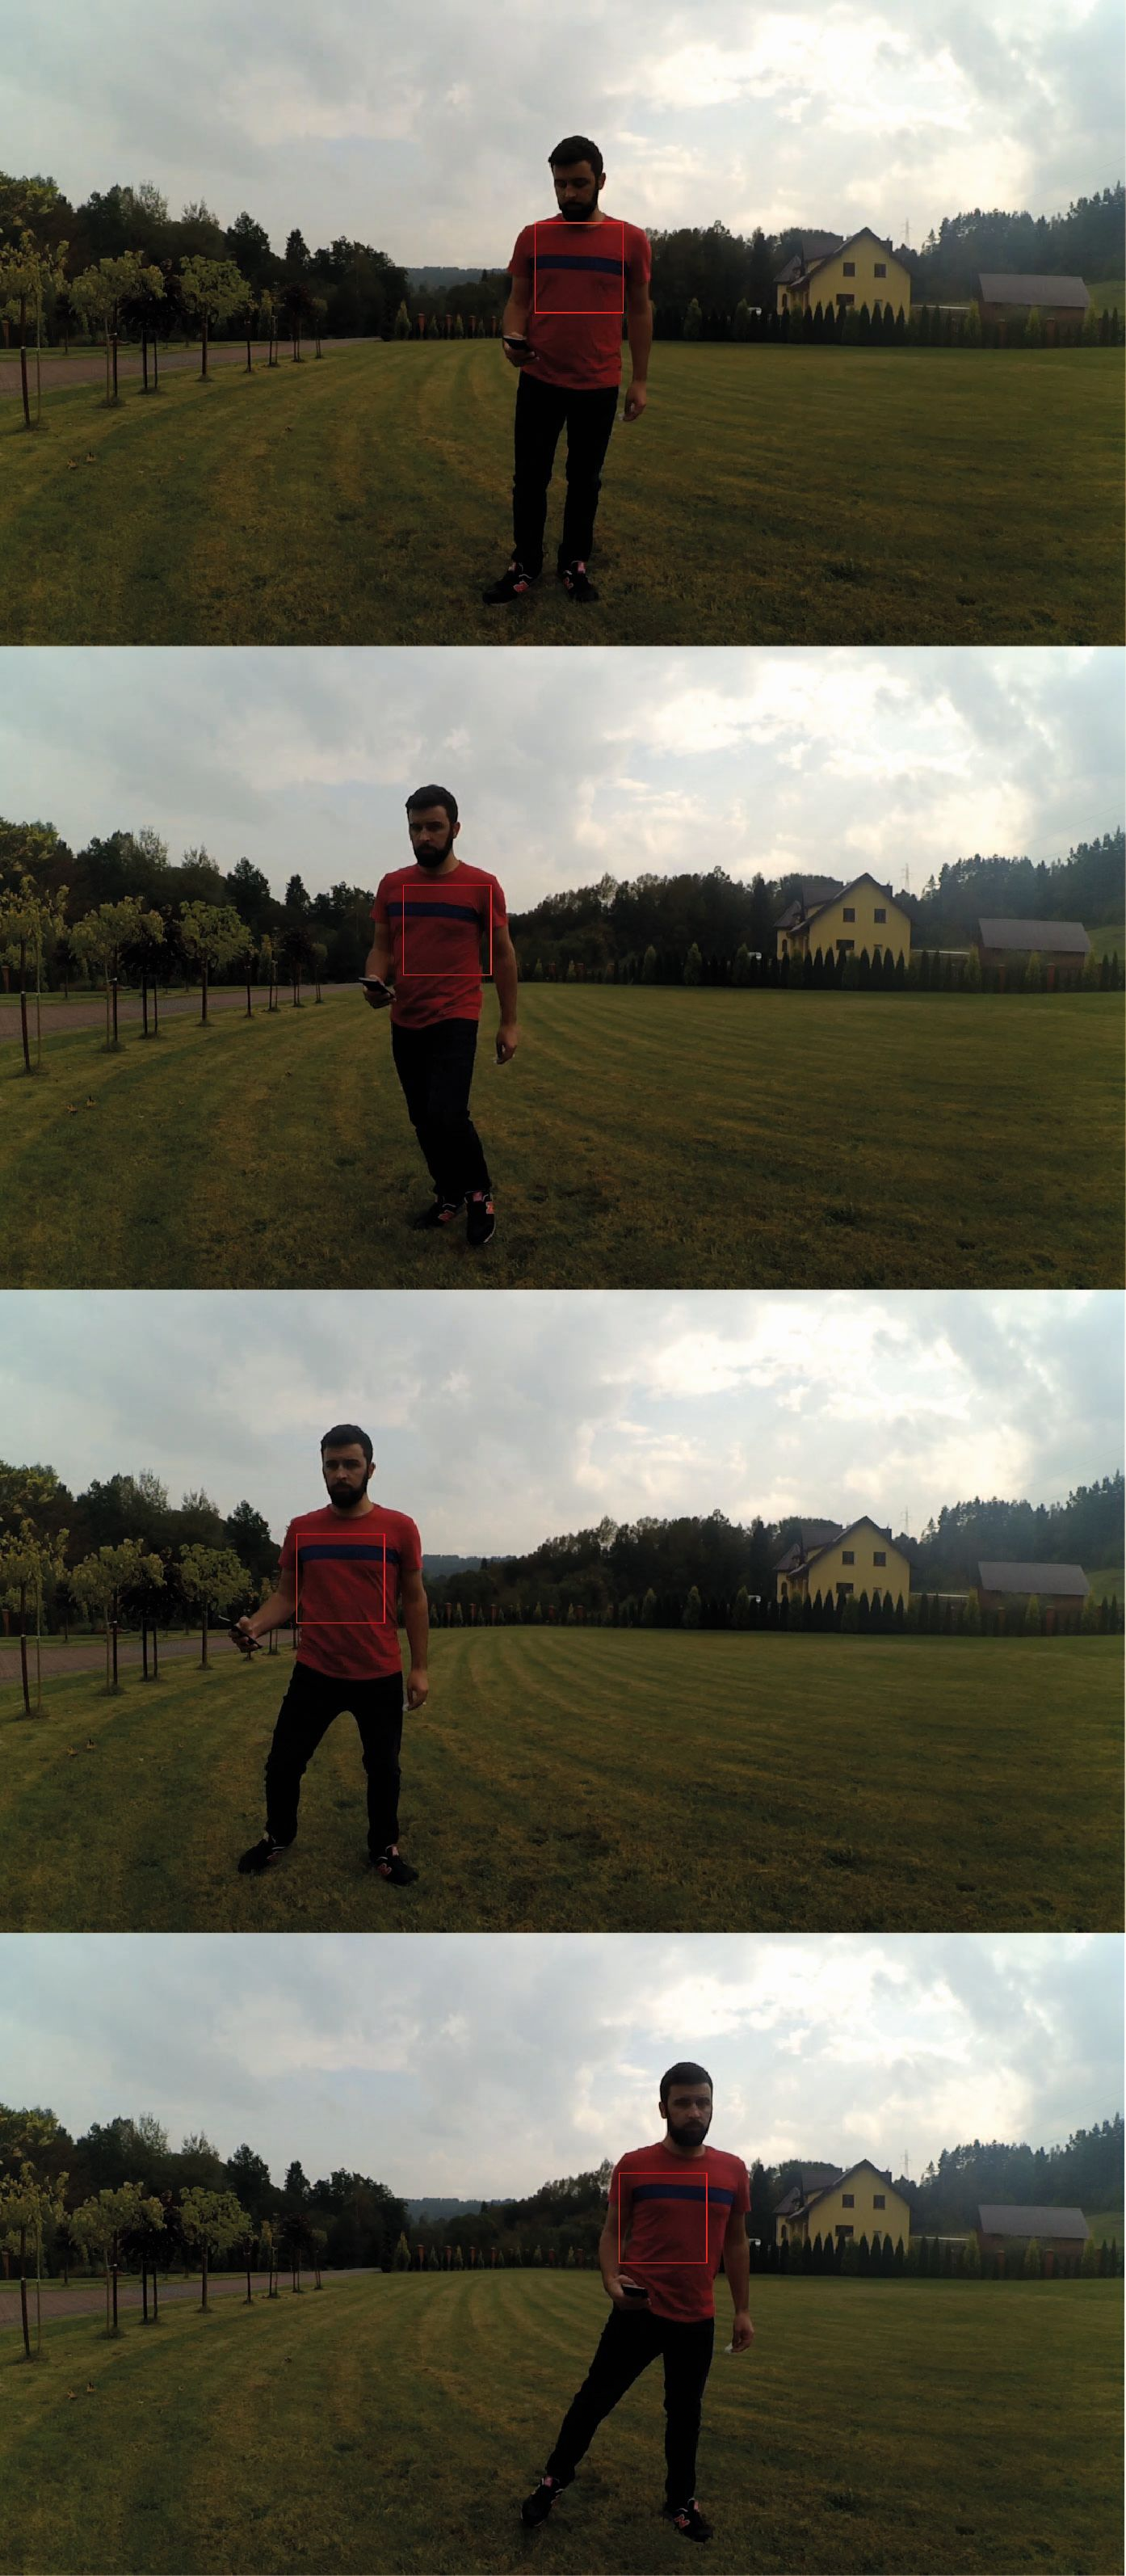
\includegraphics[width=16cm]{3_meanshift.jpg}
	\caption{Śledzenie MeanShift}
	\label{fig:meanshift_prog}
\end{figure}

%TODO 1. Obarzki mniejsze, a za to prostokąt wyraźniejszy. %ODP OK
%TODO 2. Jakieś inny test %ODP dodano w tej samej grafice
%TODO 3. Komentarz nt. działania algorymtu.

\section{Model HoG+SVM}


Głównym zadaniem modelu programowego jest próba detekcji osoby w przeskalowanym obrazie, w oparciu o obszar zainteresowań $144 \times 96$, którego środek stanowi punkt wybrany przez użytkownika. Podstawowym zadaniem jest jednak proces uczenia klasyfikatora SVM, który zostanie użyty nie tylko w modelu programowym, ale również w trakcie implementacji sprzętowej. %TODO Niejasne %ODP OK

\subsection{Uczenie}
Uczenie jest dość złożonym obliczeniowo procesem przetworzenia obrazów i ekstrakcji wektorów cech, na podstawie których powstanie płaszczyzna rozdzielająca próbki pozytywne od negatywnych. %TODO to żmudny to nie pasuje styl. %ODP OK
Przejście przez tak wielką liczbę obrazów ma charakter jednorazowy, po którym będzie dysponować się parametrami umożliwiającymi klasyfikację. 
Z tego względu nie zdecydowano się na implementację modułu uczącego w układzie FPGA -- tak ze względu na złożoność tego etapu, czas trwania procedury, jak i prawdopodobnie duży udział modułu w zużyciu zasobów logiki. 

Wybór padł na środowisko MATLAB dysponujące funkcjami wspierającymi metodę SVM. 
Skrypt korzysta z plików tekstowych zawierających listy próbek do wczytania, które ostatecznie muszą być w rozmiarze $128\times 64$. 
Wymiary próbek negatywnych mocno odbiegają od założonego wymiaru klasyfikowanego obrazu ($128\times 64$). 
Zdecydowano, iż w ich przypadku uczeniu poddany będzie obszar o wymiarach $128\times 64$ wycięty ze środka oryginałów. %TODO dlaczego raz jest 128x64 a kiedy indziej w $$. %ODP OK, nie wypatrzyłem tego. 
Proces tworzenia wektorów cech przeprowadzono zgodnie z informacjami zawartymi w rozdziale \ref{sec:HOG&SVM}; za normę blokową obrano L2 (\eqref{eq:HOG_norm3}).
Na bazie tak przygotowanych próbek powstaje tablica deskryptorów oraz druga, która przechowuje odpowiadające im wartości klas (1 lub 0). 
Z obu tablic korzysta dostępna w pakiecie Matlab funkcja \textit{svmtrain}, która zwraca strukturę \textit{svm\char`_struct} ze współczynnikami wykorzystywanymi w klasyfikacji. %TODO czego ? %ODP OK
Z kolei funkcja \textit{svmclassify} służy do klasyfikacji obrazu (a właściwie jego deskryptora). %TODO "w stanie" styl, personifikacja %ODP OK
Funkcję tę użyto w procesie testowania niezależnego zestawu danych złożonego z poprawnie sklasyfikowanych obrazów, by sprawdzić skuteczność klasyfikacji wyuczonego SVM. %TODO niejasne... raczej suteczność klasyfikiacji wyuczonego SVM. %ODP OK
Etap testowania jest dodatkowo przydatny -- pozwala na bazie eksperymentów zdefiniować optymalny rozmiar komórki (kwadratu pikseli), na bazie których liczony jest pojedynczy histogram. 
Tabela \ref{tab:HOG_cell_size} prezentuje wyniki, wśród których uwzględniony jest błąd, liczony jako stosunek liczby niepoprawnych klasyfikacji (0 zamiast i 1 zamiast 0) do liczby testowanych obrazów.
Eksperyment przeprowadzono na komputerze wyposażonym w procesor Intela klasy i7, trzeciej generacji.
\newcolumntype{P}[1]{>{\centering\arraybackslash}p{#1}}
\begin{table}[h]
	\centering
	\captionsetup{justification=centering,margin=1cm}
	
	\begin{tabular}{|P{3cm} |P{3cm} |P{4.5cm}| P{3.5cm}|}	
		\hline
		\rowcolor{lightgray} Rozmiar komórki [px] & Liczba elementów wektora cech & Błąd klasyfikacji [\%]  & Czas trwania obliczeń [s] \\ 
		\lbrack$2\times $2\rbrack			& 70308		& 3.4069		& 52min 42s		\\ 
		\hline		
		\lbrack$4\times 4$\rbrack			& 16740 	& 2.3344		& 14min 08s		\\ 
		\hline
		\lbrack$8\times 8$\rbrack			& 3780		& 3.3438		& 05min 01s		\\ 
		\hline
		\lbrack$16\times 16$\rbrack			& 756		& 5.1735		& 02min 50s		\\ 
		\hline
	\end{tabular}
	
	\caption{Skuteczność algorytmu na zbiorze testowym w zależności od wielkości pojedynczej komórki}
	\label{tab:HOG_cell_size}
\end{table}
%TODO czas trwania obliczeń. %ODP OK
%TODO jak jest liczony bład %ODP OK, nad tabelą

Okazuje się, że algorytm wykazuje największą skuteczność dla komórek o rozmiarze $4\times 4$. 
Zdecydowano się zatem na implementację algorytmu HOG w układzie FPGA właśnie dla tej wartości parametru. 
Szybkie obliczenia pokazują, że dla obrazu o wymiarach $128\times 64$ powstanie $32\times 16$ komórek, a idąc dalej, $31\times 15$ bloków po 4 histogramy po 9 wartości -- długość wektora cech będzie wynosić 16740. 
Oznacza to również, że po zakończonym procesie uczenia powstanie wektor współczynników o takiej długości. %TODO no chybo nie do końca, bo normalizacja w blokach zwiększa ten rozmiar. %ODP Mógłby Pan Doktor wyjaśnić? Ja po prostu dzielę 36 wartości danego bloku przez ich sumę+'1'. Więc wyjściem jest nadal 36 elementów na blok.

%TODO To co jest od "Uczenie" do tego momentu przenieść i zintegrować z opisem \section{Model HoG+SVM} %ODP OK


%TODO proszę to jednak podzielić osobno na uczenie i rozpoznawanie. %ODP OK

%Działanie skryptu rozpoczyna się od przeprowadzenia uczenia klasyfikatora, która bazuje na dwóch tablicach: jedna agreguje wektory cech, a druga przechowuje skojarzone z nimi klasy (0 lub 1). 
%Wykorzystywana baza obrazów wyposażona jest w pliki z ich listami (osobno dla pozytywnych i negatywnych przykładów), co umożliwia proste wczytywanie kolejnych próbek. 
%Oczekuje się tu rozmiaru $128\times 64$ pikseli, jednak niektóre (zwłaszcza negatywne) obrazy są za duże -- przeprowadza się tutaj wycięcie fragmentu o podanym wyżej rozmiarze ze środka każdej próbki. Kolejnymi etapami dla takiego obszaru są kolejno: konwersja do odcieni szarości oraz obliczenie wektora cech. 
 %TODO styl. potrzeby.. niepotrzebnie %ODP OK

\subsection{Rozpoznawanie}
Po uzyskaniu struktury ze współczynnikami można podjąć się klasyfikacji obszarów z obrazów wczytanych przez użytkownika.

Napisany w tym celu skrypt rozpoczyna działanie od wczytania obrazu wejściowego. 
Po zdefiniowaniu punktu będącego środkiem obszaru zainteresowań następuje realizacja algorytmu HOG+SVM dla każdej z 5 zdefiniowanych wcześniej skal.
Pierwszym krokiem jest obliczenie $5\times 9$ wektorów cech na fragmencie $144 \times 96$ -- celem jest znalezienie jak najlepszego wyniku detekcji.  %TODO niejasne, i styl z "planu".  %ODP OK
%TODO Czy to jest tylko w jednej skali licznone ? %ODP Nie, dla wielu - wyświetlany jest najlepszy wynik - wyświetlanie wszystkich wyników poniżej 0 wygląda dość nieczytelnie
Idąc za przykładem wbudowanej w MATLAB funkcji \textit{svmclassify}, następuje klasyfikacja każdego obliczonego wektora cech. Proces ten jest powtarzany dla każdej z wcześniej określonych skal. 
Końcowym etapem jest wyświetlenie oryginalnego obrazu w kolorze, z naniesionymi konturami: obszarów zainteresowań $144\times 96$, oraz pozytywnych detekcji o wymiarach $128\times 64$ -- przeskalowanych do rzeczywistego rozmiaru. Finalna detekcja jest obliczana na podstawie najlepszego (najniższego) wyniku klasyfikacji z zebranych wyników analiz wszystkich skal.

Przykłady detekcji w pojedynczych skalach zaprezentowano na rysunkach \ref{fig:SVMmodel}, \ref{fig:SVMmodel_2_5} oraz \ref{fig:SVMmodel_3}.
Różowym konturem oznaczono okno detekcji $144 \times 96$, natomiast na czerwono zakreślono ostateczne obszary $128\times 64$ pozytywnie wybrane przez klasyfikator. Przedstawiono również tabele z wynikami klasyfikacji poszczególnych deskryptorów. Pogrubione zostały pozytywne wyniki detekcji.%TODO ale trzeba napisać co to za wyniki. %ODP OK
\begin{figure}[]
	\centering
	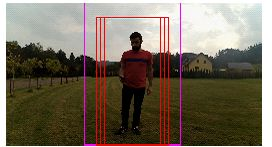
\includegraphics[width=10cm]{3_SVM_model.jpg}
	\caption{Detekcja na oknie wewnątrz obrazu (skala: 5)}
	\label{fig:SVMmodel}
\end{figure}

\newcolumntype{P}[1]{>{\centering\arraybackslash}p{#1}}
\begin{table}[]
	\centering
	\caption{Tabela z wynikami dla $5 \times 9$ detekcji z rysunku \ref{fig:SVMmodel}}
	\begin{tabular}{|P{1.2cm} |P{1.2cm} |P{1.2cm} |P{1.2cm} |P{1.2cm} |P{1.2cm} |P{1.2cm} |P{1.2cm} |P{1.2cm} |}
		
		\hline
$1.4357$ &   $1.0343$  &  $1.4887$  &  $1.1960$  &  $1.1270$  &  $1.2742$ &   $0.6366$  &  $0.9465$  &  $0.8936$ \\ \hline
$0.9876$ &   $1.1790$  &  $1.7361$  &  $1.4707$  &  $1.0850$  &  $1.2012$ &   $1.2482$  &  $1.5096$  &  $1.2834$ \\ \hline
$1.4188$ &   $1.3449$  &  $2.1487$  &  $1.8528$  &  $0.9389$  &  $0.7458$ &   $1.0194$  &  $1.5121$  &  $1.7702$ \\ \hline
$1.5967$ &   $2.0461$  &  $1.7974$  &  $1.1585$  &  $0.6553$  &  $0.6955$ &   $0.5781$  &  $1.6717$  &  $1.3235$ \\ \hline
$1.2971$ &   $2.0113$  &  $1.2289$  & $\textbf{-0.0191}$  & $\textbf{-0.5477}$  & $\textbf{-1.0460}$ &   $0.2423$  &  $1.0235$  &  $1.7798$ \\ \hline		
	\end{tabular}
	\label{tab:scale_window_cover_5}
\end{table}

\begin{figure}[h]
	\centering
	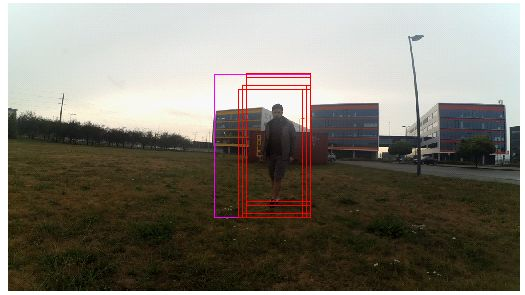
\includegraphics[width=12cm]{3_SVM_model_2_5.jpg}
	\caption{Detekcja na oknie wewnątrz obrazu (skala: 2.5)}
	\label{fig:SVMmodel_2_5}
\end{figure}

\newcolumntype{P}[1]{>{\centering\arraybackslash}p{#1}}
\begin{table}[h]
	\centering
	\caption{Tabela z wynikami dla $5 \times 9$ detekcji z rysunku \ref{fig:SVMmodel_2_5}}
	\begin{tabular}{|P{1.2cm} |P{1.2cm} |P{1.2cm} |P{1.2cm} |P{1.2cm} |P{1.2cm} |P{1.2cm} |P{1.2cm} |P{1.2cm} |}
		
		\hline
    $2.1223$  &  $1.9234$  &  $1.8072$ & $1.8854$  &  $1.6932$ &  $1.5320$  & $ 0.5443$ &  $ 0.2648$  & $\textbf{-0.0366}$ \\ \hline
$1.9547$  &  $2.5649$  &  $1.6400$ & $1.7075$  &  $1.1940$ &  $1.5821$  & $ 0.6492$ &  $ 0.2804$  & $\textbf{-0.0880}$ \\ \hline
$2.5165$  &  $2.7328$  &  $2.3592$ & $2.2650$  &  $2.1196$ &  $1.1509$  & $ 0.8788$ &  $ 0.6314$  & $ 0.1222$ \\ \hline
$2.4744$  &  $2.8618$  &  $2.7310$ & $2.6338$  &  $2.1627$ &  $1.4763$  & $ 0.4520$ &  $\textbf{-0.7166}$  & $\textbf{-1.1757}$ \\ \hline
$2.6806$  &  $2.4200$  &  $2.2032$ & $1.6812$  & $1.9216$ &  $0.9355$  & $\textbf{-0.0505}$ &  $\textbf{-1.3537}$  & $\textbf{-1.3712}$ \\ \hline	
	\end{tabular}
	\label{tab:scale_window_cover_2_5}
\end{table}

\begin{figure}[h]
	\centering
	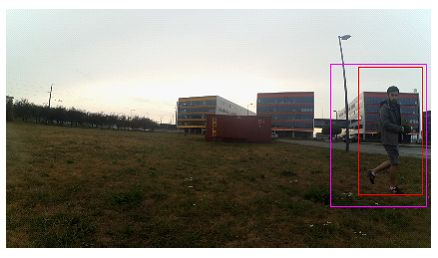
\includegraphics[width=12cm]{3_SVM_model_3.jpg}
	\caption{Detekcja na oknie wewnątrz obrazu (skala: 3)}
	\label{fig:SVMmodel_3}
\end{figure}


\newcolumntype{P}[1]{>{\centering\arraybackslash}p{#1}}
\begin{table}[h]
	\centering
	\caption{Tabela z wynikami dla $5 \times 9$ detekcji z rysunku \ref{fig:SVMmodel_3}}
	\begin{tabular}{|P{1.2cm} |P{1.2cm} |P{1.2cm} |P{1.2cm} |P{1.2cm} |P{1.2cm} |P{1.2cm} |P{1.2cm} |P{1.2cm} |}
	\hline	
    $1.8159$  &  $1.8308$  &  $1.7164$  &  $1.4868$  &  $1.1955$  &  $1.1542$  &  $0.8346$  & $ 0.4625$   & $0.6144$ \\ \hline
$2.3357$  &  $2.6091$  &  $2.0017$  &  $2.0776$  &  $2.2638$  &  $1.8270$  &  $0.6915$  & $\textbf{-0.0323}$  &  $0.6554$ \\ \hline
$2.3233$  &  $2.4182$  &  $1.9292$  &  $2.1127$  &  $1.8924$  &  $1.7307$  &  $0.8044$  & $ 0.3019$  &  $0.7611$ \\ \hline
$1.5705$  &  $1.6276$  &  $1.5120$  &  $1.7848$  &  $1.6619$  &  $1.7323$  &  $0.4511$  & $ 0.8625$  &  $1.1717$ \\ \hline
$1.4874$  &  $1.8153$  &  $1.0768$  &  $1.2884$  &  $1.0186$  &  $1.8310$  &  $0.8986$  & $ 0.6349$  &  $1.1386$ \\ \hline
	\end{tabular}
	\label{tab:scale_window_cover_3}
\end{table}

%TODO Czy w jakiś sposób obliczena jest finalna detekcja ? Oraz jak to się przekłada na odległosć. %ODP opisano wyżej jak jest liczona
%TODO Dobrze by było jeszcze zamieścić taki eksperytment - sekwencja na której Pan oddala się od kamery i korespondujące odległości. %Taki ekperyment zrobiłem 'na żywo', z wyjściem video na monitor
%TODO Nie wiem czy nie warto rozważyć przetwarzania w więcej niż jednej skali.... albo wszystkich albo przynajmniej sąsiednich (pamiętając tą najlepszą). %ODP Tak robiłem, ale wizualnie to nie ma sensu, bo jest zbyt wiele detekcji i obraz staje się nieczytelny

%TODO BTW, Na takiej sekwencji można też od razu sprawdzić działanie meanshifta. Albo nagrać jeszcze taką gdzie oprócz do przodu idzie się w lewo i prawo... %ODP Nie mam modelu programowego łączącego oba algorytmy, nie wyrobiłem czasowo żeby go połączyć
\chapter{Implementacja sprzętowo-programowa systemu wizyjnego}

Jednym z pierwszych zadań związanych z realizacją projektu było określenie sposobu implementacji systemu wizyjnego.
Po uwzględnieniu wysokiej złożoności obliczeniowej algorytmów, a także ograniczeń związanych z miejscem działania systemu wizyjnego (platforma UAV) -- takich jak rozmiar układu i pobór mocy -- postanowiono wybrać podejście oparte o implementację sprzętowo-programową. W przeciwieństwie do programu komputerowego, urządzenie realizujące odpowiednio zaimplementowany algorytm ze wsparciem sprzętowym cechuje się większą szybkością działania. Wadą takiego rozwiązania jest koszt i czas jego przygotowania. 

W pracy zdecydowano się wykorzystać heterogeniczny układ Zynq opisany w dalszej części rozdziału. 

%TODO 2 trochę się nie zroumieliśmy. Chodziło mi o to, dlaczego sprzętowa w tym konkrentym przypadku. Że algorytm złożony, że na drona itp... 
% I tu też, że ZYnq, bo potem Pan to opisuje. %ODP OK


\section{Układy Zynq}


Najważniejszym i najbardziej czasochłonnym elementem pracy była sprzętowa implementacja algorytmów detekcji i śledzenia. 
W dzisiejszych czasach istnieje możliwość skorzystania z przeróżnych platform obliczeniowych, które dzieli się, jak przedstawiono poniżej:
\begin{itemize}
	\item brak możliwości zmiany funkcjonalności po wyprodukowaniu układu:
	\begin{itemize}
		\item procesory ASIP (ang. \textit{Application Specific Instruction Set Processor}) -- zaprojektowane z dedykowanym zestawem instrukcji		
		\item układy ASIC (ang. \textit{Application Specific Integrated Circuit}) -- zaprojektowane do realizacji określonej z góry zadań
		\item procesory ogólnego przeznaczenia GPP (ang. \textit{General Purpose Processor})
		\item procesory graficzne GPU (ang. \textit{Graphics Processing Unit})
		\item procesory sygnałowe DSP (ang. \textit{Digital Signal Processor})
	\end{itemize}
	\item z możliwością konfiguracji po procesie produkcyjnym - układy FPGA (ang. \textit{Field-Programmable Gate Array}) oraz CPLD (ang. \textit{Complex Programmable Logic Device})
\end{itemize}

Specjalizowane układy ASIC są niestety drogie w prototypowaniu. 
Proces ten oznacza stworzenie układu scalonego od podstaw, i biorąc pod uwagę brak możliwości rekonfiguracji, musi uwzględniać szereg działań związanych z zapewnieniem poprawności działania (tj. testowania) przed przekazaniem do produkcji. 
Procesory CPU, czy DSP nie pozwalają na przetworzenie tak wielkiej ilości danych w czasie rzeczywistym -- szczególnie dla obrazów o wysokiej rozdzielczości. Ponadto charakteryzują się względnie dużym zużyciem energii.

Z kolei druga z wymienionych grup urządzeń ma atut polegający na możliwości zmiany architektury układu oraz zrównoleglenia obliczeń tak bardzo, jak tylko pozwala na to liczba dostępnych zasobów.
Dodatkowo -- i paradoksalnie zarazem -- urządzenia te charakteryzują się stosunkowo niskim zapotrzebowaniem na energię. 
Ma to istotne znaczenie, mając na uwadze światowy trend poszukiwań energooszczędnych rozwiązań w każdej branży --  a zwłaszcza na rynku dronów, których czas lotu jest przeważnie ograniczony pojemnością baterii do kilkunastu minut.
Obszary, w których FPGA znajduje zastosowanie to między innymi:
\begin{itemize}
	\item studia dźwiękowe,
	\item telekomunikacja,
	\item przemysł motoryzacyjny/zbrojeniowy/lotniczy/kosmiczny,
	\item szyfrowanie i przetwarzanie danych,
	\item aparatura medyczna,
	\item systemy wizyjne.
\end{itemize}
To wszystko nie oznacza jednak, że układy FPGA nie są pozbawione wad. 
Przykładowo, realizacja niektórych rodzajów algorytmów (głównie rekurencyjnych) jest utrudniona i mało efektywna. 
Ponadto, sam proces rozwoju konkretnej architektury nie należy do najprostszych i może wymagać potwierdzenia funkcjonalności na kilka sposobów:
\begin{itemize}
	\item porównanie wyników z modelem stworzonym w innym, konwencjonalnym środowisku (MATLAB, OpenCV). Przykładowo, pozwala to zweryfikować poprawność logiki w układzie rekonfigurowalnym, która jest tworzona w oparciu o zapis stałoprzecinkowy. Dla wspólnego scenariusza testowego, różnice pomiędzy poszczególnymi wartościami nie powinny być większe niż akceptowalny poziom błędu. %TODO 2 raczej różnice pomiędzy wartościami.. jakoś to ciut inaczej ująć. %ODP OK
	\item symulacja HDL na komputerze -- umożliwia weryfikację projektu lub jednego z modułów poprzez określenie wymuszeń sygnałów w~testowym module zewnętrznym, tzw. \textit{testbenchu}. Proces ten aktualizuje stan logiczny wszystkich obiektów (modułów) w określonym odstępie czasu, przykładowo 1 ps.
	\item weryfikacja wybranych sygnałów w układzie przy użyciu zintegrowanego analizatora logicznego --  SignalTap dla urządzeń firmy Intel (dawniej Altera), ILA dla układów firmy Xilinx. Oznaczając w budowanym projekcie odpowiednie sygnały i wykorzystując protokół JTAG, możliwe jest skomunikowanie się z układem i akwizycja zdefiniowanej liczby próbek każdego z elementów. Na szczególną uwagę zasługuje opcja wyzwolenia procesu akwizycji spełnieniem określonego warunku (powiązanego ze stanem dostępnych sygnałów). 
\end{itemize}

Część problemów bywa z czasem rozwiązywana przez producentów. 
Stopień skomplikowania projektu można znacznie zredukować, wykorzystując dostarczaną z oprogramowaniem własność intelektualną -- odpowiednio skonfigurowane tzw. IP Core'y -- i łącząc sygnały pomiędzy nimi na diagramach graficznych. 
Co więcej, narzędzie Vivado High-Level Synthesis (HLS) oferuje możliwość konwersji języka C/C++ do technologii FPGA, upraszczając proces powstawania architektury. 

Postępująca zwłaszcza w ostatnich latach integracja i zmniejszanie procesu technologicznego pozwoliły na stworzenie układów łączących logikę programowalną (FPGA) oraz dwurdzeniowy procesor ARM. 
Układ, na którym oprócz jednostki obliczeniowej znajdują się różne peryferia, nosi nazwę układu heterogenicznego, w branży bardziej znanego jako \textit{System on a Chip} (SoC).
Dzięki magistrali (przykładowo AXI) zapewniającej szybką wymianę danych pomiędzy blokami, taki układ pozwala łączyć możliwość zrównoleglania obliczeń, którą daje logika programowalna (\textit{ang. PL - Programmable Logic}) oraz prostotę rozwoju oprogramowania uruchamianego na procesorze (\textit{ang. PS - Processing System}). 
W tej ostatniej części istnieje możliwość pracy w systemie operacyjnym (jednym ze specjalnych dystrybucji systemu Linux) lub nawet stworzenia konfiguracji opartej o wieloprocesorowość asynchroniczną (ang. AMP -- \textit{asynchronous multiprocessing}), która pozwala wykorzystać oba dostępne rdzenie procesora do niezależnych celów. 
Poza prostym przypadkiem jak praca z dwiema równoległymi aplikacjami, możliwe jest nawet działanie w konfiguracji Linux+RTOS (ang. real-time operating system -- system operacyjny czasu rzeczywistego)) \cite{AMP}. %TODO 2 - rozwinąć RTOS %ODP OK
Warto tu zauważyć, że narzędzia syntezy logiki od dawna oferowały możliwość stworzenia softprocesorów w układach FPGA (Altera -- Nios, Xilinx -- MicroBlaze), jednak te rozwiązania istotnie ograniczały dostępne zasoby, a częstotliwość taktowania takich komponentów rzadko przekraczała 200 MHz. 

Powyższa charakterystyka przekonuje, że układy FPGA, a zwłaszcza SoC mógłby być szczególnie doceniony na platformie latającej, gdyż byłby w stanie sprostać wymaganiom stawianym przez zadanie przetwarzania obrazu w czasie rzeczywistym, a dzięki niewielkim wymiarom i niskiemu zużyciu energii nie stanowiłby wielkiego obciążenia przy i tak już mocno ograniczonym czasie lotu na jednej baterii. 

W pracy zdecydowano się wykorzystać układ Zynq SoC firmy Xilinx. 
O wyborze zadecydował nie tylko charakter projektu wymagający zrównoleglenia wykonywanych obliczeń, ale też niski pobór mocy oraz obecność dwóch rdzeni procesora ARM do realizacji części zadań. Sledzenie za pomocą algorytmów MeanShift oraz HOG+SVM wymaga bowiem przetwarzania danych w czasie rzeczywistym, ale już sterowanie pracą obu metod może być wykonywane w sposób programowy.  %TODO 2 - może warto przypomnieć algorytmy ?  %ODP OK
Oczywiście, ze względu na poziom skomplikowania montażu układu Zynq nie podjęto decyzji o prototypowaniu własnego obwodu drukowanego, lecz wykorzystano niewielki, lecz bogaty w peryferia zestaw PYNQ z układem Zynq SoC XC7Z020. 
Oprogramowaniem wspierającym rozwój architektury na to urządzenie jest pakiet Xilinx Vivado + SDK. Dostarczana z nim własność intelektualna (tzw. moduły IP) jest tworzona w oparciu o popularny standard wymiany danych - magistralę AXI (ang. Advanced eXtensible Interface). Pozwala ona stworzyć jednolitą architekturę tworzonego systemu bazującego na adresowym dostępie do danych.

Część PS układu XC7Z020 jest wyposażona w:
\begin{itemize}
	\item dwurdzeniowy procesor Cortex-A9 taktowany zegarem 650MHz,
	\item kontroler pamięci DDR3 z 8 kanałami DMA (ang. Direct Memory Access) oraz 4 wydajnymi portami AXI3, %TODO 2 AXI4 ? %ODP szybkie porty HP są oparte o AXI3
	\item wydajne kontrolery 1Gb Ethernet, USB 2.0, SDIO (ang. Secure Digital Input Output),
	\item kontrolery SPI, UART, CAN, I2C.
\end{itemize}
Część PL stanowi logika z rodziny urządzeń Artix-7, z następującymi parametrami:
\begin{itemize}
	\item 13300 elementów \textit{slice}, każdy wyposażony w 4 sześcioportowe tablice LUT (ang. Look-Up Table) oraz 8 przerzutników, %TODO 2 skrót LUT %ODP OK
	\item 630KB szybkiej pamięci Block RAM,
	\item 4 obszary zarządzania zegarami, każdy z układem PLL (ang. Phase Locked Loop) i~MMCM (ang. Mixed-Mode Clock Manager),
	\item 220 elementów DSP (ang. digital signal processing -- cyfrowe przetwarzanie sygnałów),
	\item konwerter analogowo-cyfrowy (XADC -- ang. Xilinx Analog-to-Digital Converter).
\end{itemize}

Poniżej przedstawiono pozostałe najważniejsze parametry platformy PYNQ:
\begin{itemize}
	\item sygnał zegarowy o częstotliwości $125$MHz
	\item 512 MB pamięci DDR3 z 16-bitową magistralą o przepustowości 1050Mbps,
	\item 16MB pamięci flash,
	\item slot na kartę MicroSD,
	\item złącza: MicroUSB z interfejsem JTAG, USB, Ethernet, 2x PMOD (ang. Peripheral Module), 3.5mm audio, we/wy HDMI,
	\item 4 przyciski, 2 przełączniki, 4 jednokolorowe diody LED oraz 2 RGB LED.
	\item możliwość zasilania bateryjnego, poprzez USB lub dołączony zasilacz 12V.
\end{itemize}

\begin{figure}[h]
	\centering
	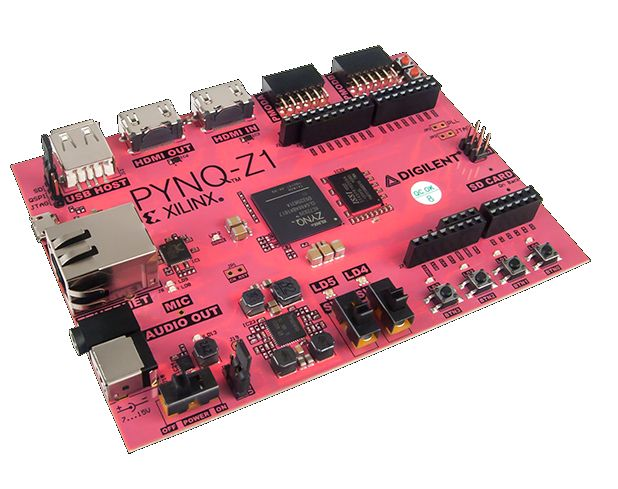
\includegraphics[width=9cm]{4_PYNQ.jpg}
	\caption{Platforma PYNQ z układem Zynq SoC XC7Z020 w centrum}
	\label{fig:PYNQ}
\end{figure}

%TODO 2 1. Takie mniej oczwysite skórty wypada rozwinąć (oczywsite to USB, LED). 2. Kilka zdań o AXI ? %ODP opisano wyżej

\section{Tor wizyjny w części PL} 
\label{sec:counter}


Podstawowym komponentem toru wizyjnego jest moduł odbierający sygnał wideo z zewnętrznego źródła -- w tym wypadku poprzez port HDMI -- i zapewniający jego poprawne zdekodowanie go do podstawowej, użytecznej przestrzeni barw RGB. 
Taki zestaw sygnałów może być w prosty sposób wykorzystany w tworzonych algorytmach. 
Opcjonalne i zalecane jest również wyprowadzenie przetworzonego sygnału RGB na monitor, co pozawala zweryfikować poprawność tworzonej architektury. 
Wyżej opisany szkielet został stworzony w tzw. \textit{Block Designie}, a poza modułami firmy Xilinx wykorzystano konwertery DVI$\rightarrow$RGB oraz RGB$\rightarrow$DVI dostarczone przez firmę Digilent -- producenta zestawu PYNQ. 
Ponadto, podstawowym zegarem systemu jest dostarczany z karty PYNQ zegar o częstotliwości $125$MHz, na bazie którego powstaje szereg pozostałych zegarów. 
 
W zadaniu śledzenia i detekcji zdecydowanie najważniejszym parametrem jest częstotliwość próbkowania sygnału wideo ze względu na potrzebę analizy jak najmniejszych ruchów obiektu. 
Kolejnym parametrem jest rozdzielczość -- obiekt na obrazie o wyższej rozdzielczości będzie opisywany większą liczbą pikseli, jednak niekorzystnie wpływa to na zużycie zasobów układu -- wymagane jest osiągnięcie pewnego kompromisu. 
Z tego względu założono, że transmisja z kamery i przetwarzanie wideo będzie się odbywać w oparciu o standard $1280\times 720/60$\textit{fps}.
%TODO 2 może napisać, ze to 1280x720. %ODP OK

Sygnały wideo, które można wyodrębnić po zdekodowaniu, to:
\begin{itemize}
	\item zegar taktujący pikseli ($74.25$MHz),
	\item kolor czerwony R (8 bitów),
	\item kolor zielony G (8 bitów),
	\item kolor niebieski B (8 bitów),
	\item synchronizacja pozioma -- poziom wysoki sygnalizuje koniec poziomej linii,
	\item synchronizacja pionowa -- poziom wysoki sygnalizuje koniec klatki obrazu,
	\item sygnał aktywny -- poziom wysoki sygnalizuje obecność poprawnego piksela.
\end{itemize}

Uwzględniając narzut związany z~polami wygaszania pionowego i~poziomego, ostateczna częstotliwość taktowania piksela wynosi w tym przypadku $74.25$MHz. 
To właśnie ten zegar, nazywany dalej w pracy \textit{\boldmath pixel\char`_clk}, steruje pracą modułów odpowiadających za potokowe przetwarzanie obrazów w części PL.
Ilustracja \ref{fig:720_frame} przedstawia zapis klatki z sygnałami sterującymi, gdzie jednostką jest cykl zegara taktującego piksel. %TODO 2 no nie wiem jak się tu jeszcze uchowałą "poniższa". %ODP :)

\begin{figure}[h]
	\centering
	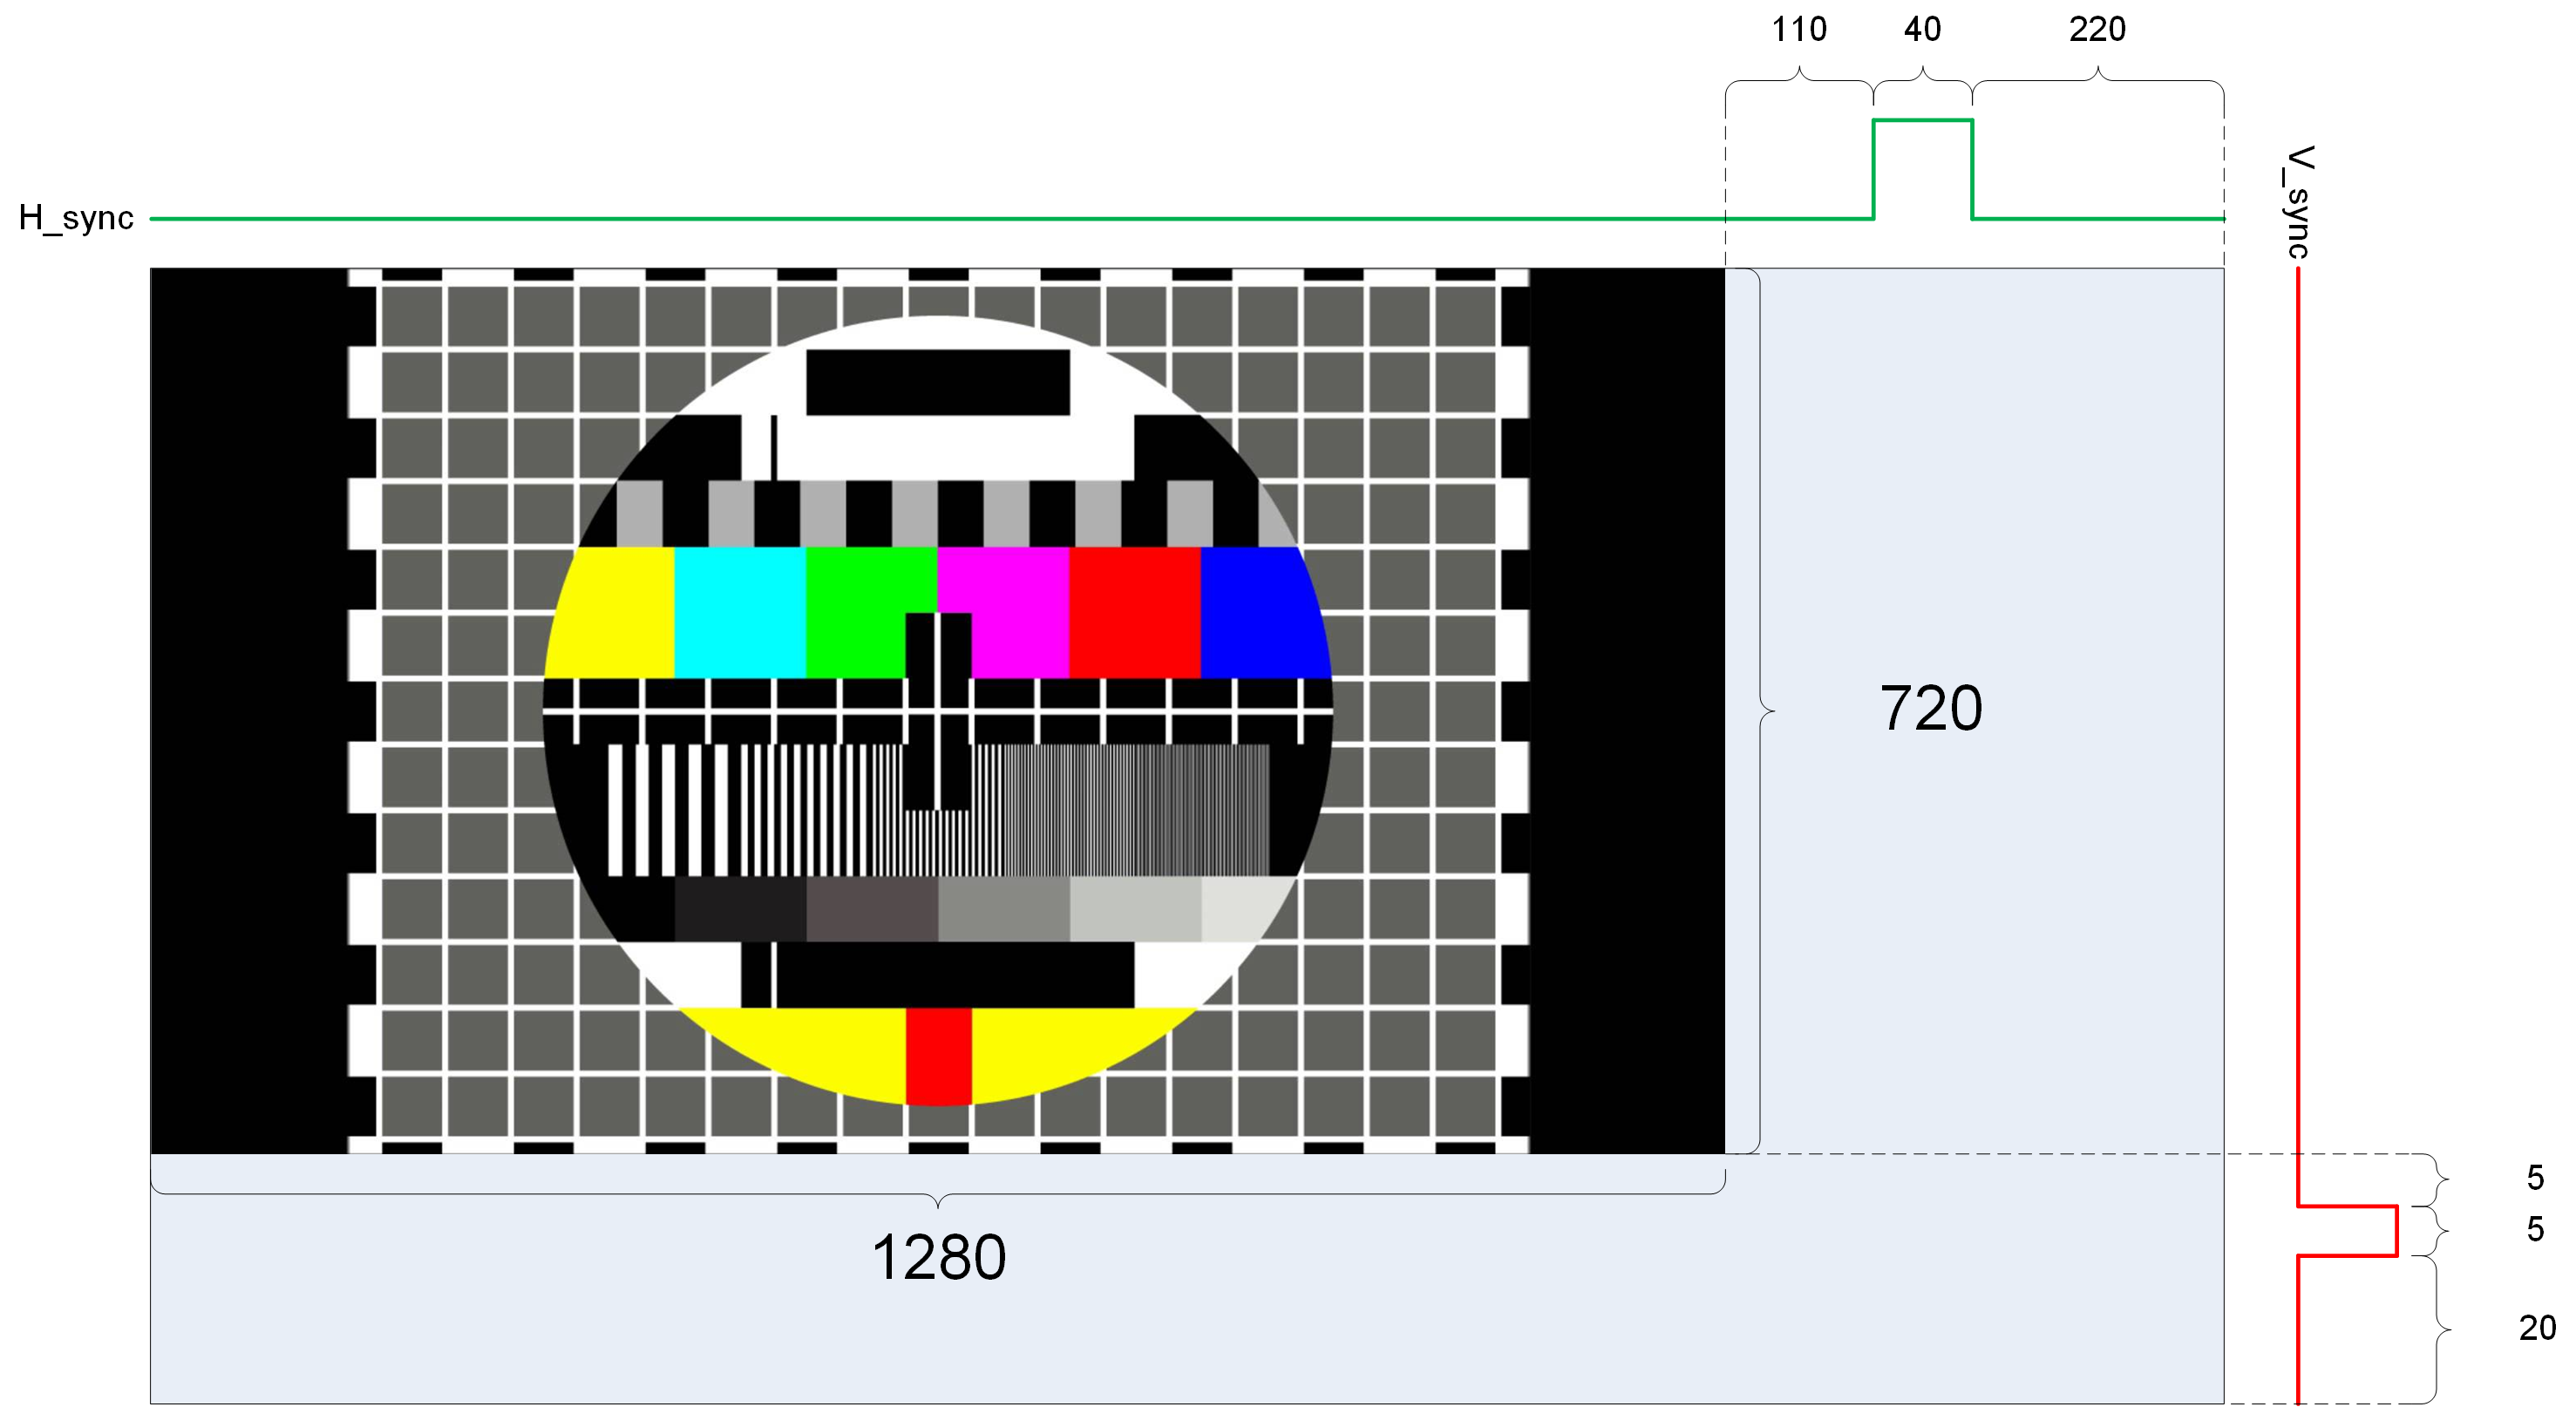
\includegraphics[width=17cm]{4_720p.png}
	\caption{Schemat zapisu klatki w rozdzielczości $720p$}
	\label{fig:720_frame}
\end{figure}

Algorytmy opisane w dalszej części pracy będą często wymagać informacji o aktualnym położeniu piksela na właściwym obrazie. %TODO 2 raczej wymagać takiej informacji. %ODP OK
Stworzono w tym celu licznik obliczający tę pozycję dla osi pionowej i poziomej w oparciu o długości trwania sygnałów kontrolnych z rysunku \ref{fig:720_frame}. 

 
\section{Implementacja algorytmu MeanShift}

Działanie algorytmu MeanShift rozpoczyna się po otrzymaniu sygnału \textit{meanshift\_en} i polega na zdefiniowaniu wzorca. Uwzględniając parametry optyczne kamery, jak i rozdzielczość wejściową materiału wideo, podjęto decyzję o śledzeniu obszaru o wymiarach $100 \times 100$ pikseli.
Na jego bazie obliczana i zapisywana jest funkcja gęstości prawdopodobieństwa, tworzona w oparciu o jądro i jego gradient, które wygenerowano w procesie inicjalizacji. 
Następnie porównuje się ją z funkcjami gęstości prawdopodobieństwa kandydatów uzyskanych w kolejnych ramkach obrazu. By uwzględnić ruch obiektu pomiędzy klatkami, zapisywany jest wówczas fragment poszerzony o otoczenie 15 pikseli z każdej strony -- o wymiarach $130 \times 130$ pikseli. 
Na tej podstawie obliczany jest wektor MeanShift, który określa przesunięcie kandydata i jednocześnie definiuje obszar następnych poszukiwań.
Ten etap jest wykonywany w sposób iteracyjny, tj. powiększa precyzję przesunięcia śledzonego obszaru, wykorzystując zapisane sąsiedztwo obszaru w celu obliczenia aktualnej funkcji gęstości prawdopodobieństwa. 
Po określonej liczbie iteracji podejmowana jest akwizycja obszaru kandydata z kolejnej klatki.
%TODO 2 OK, choć jakby Pan to jeszcze przeczytał i dogładził. %ODP OK

Analizując możliwości pracy układu w oparciu o testy symulacyjne okazało się, że algorytm jest w stanie pracować z częstotliwością \textit{60Hz}. Może bowiem przetworzyć rozpatrywany fragment z bieżącej klatki obrazu w czasie ok. 4ms, co przy okresie trwania ramki wynoszącym 16.(6)ms  pozwala zakończyć analizę przed zapisem obszaru z kolejnej ramki.  
Ogólny schemat blokowy jest przedstawiony na rysunku \ref{fig:MS_scheme_FPGA}.
\begin{figure}[h]
	\centering
	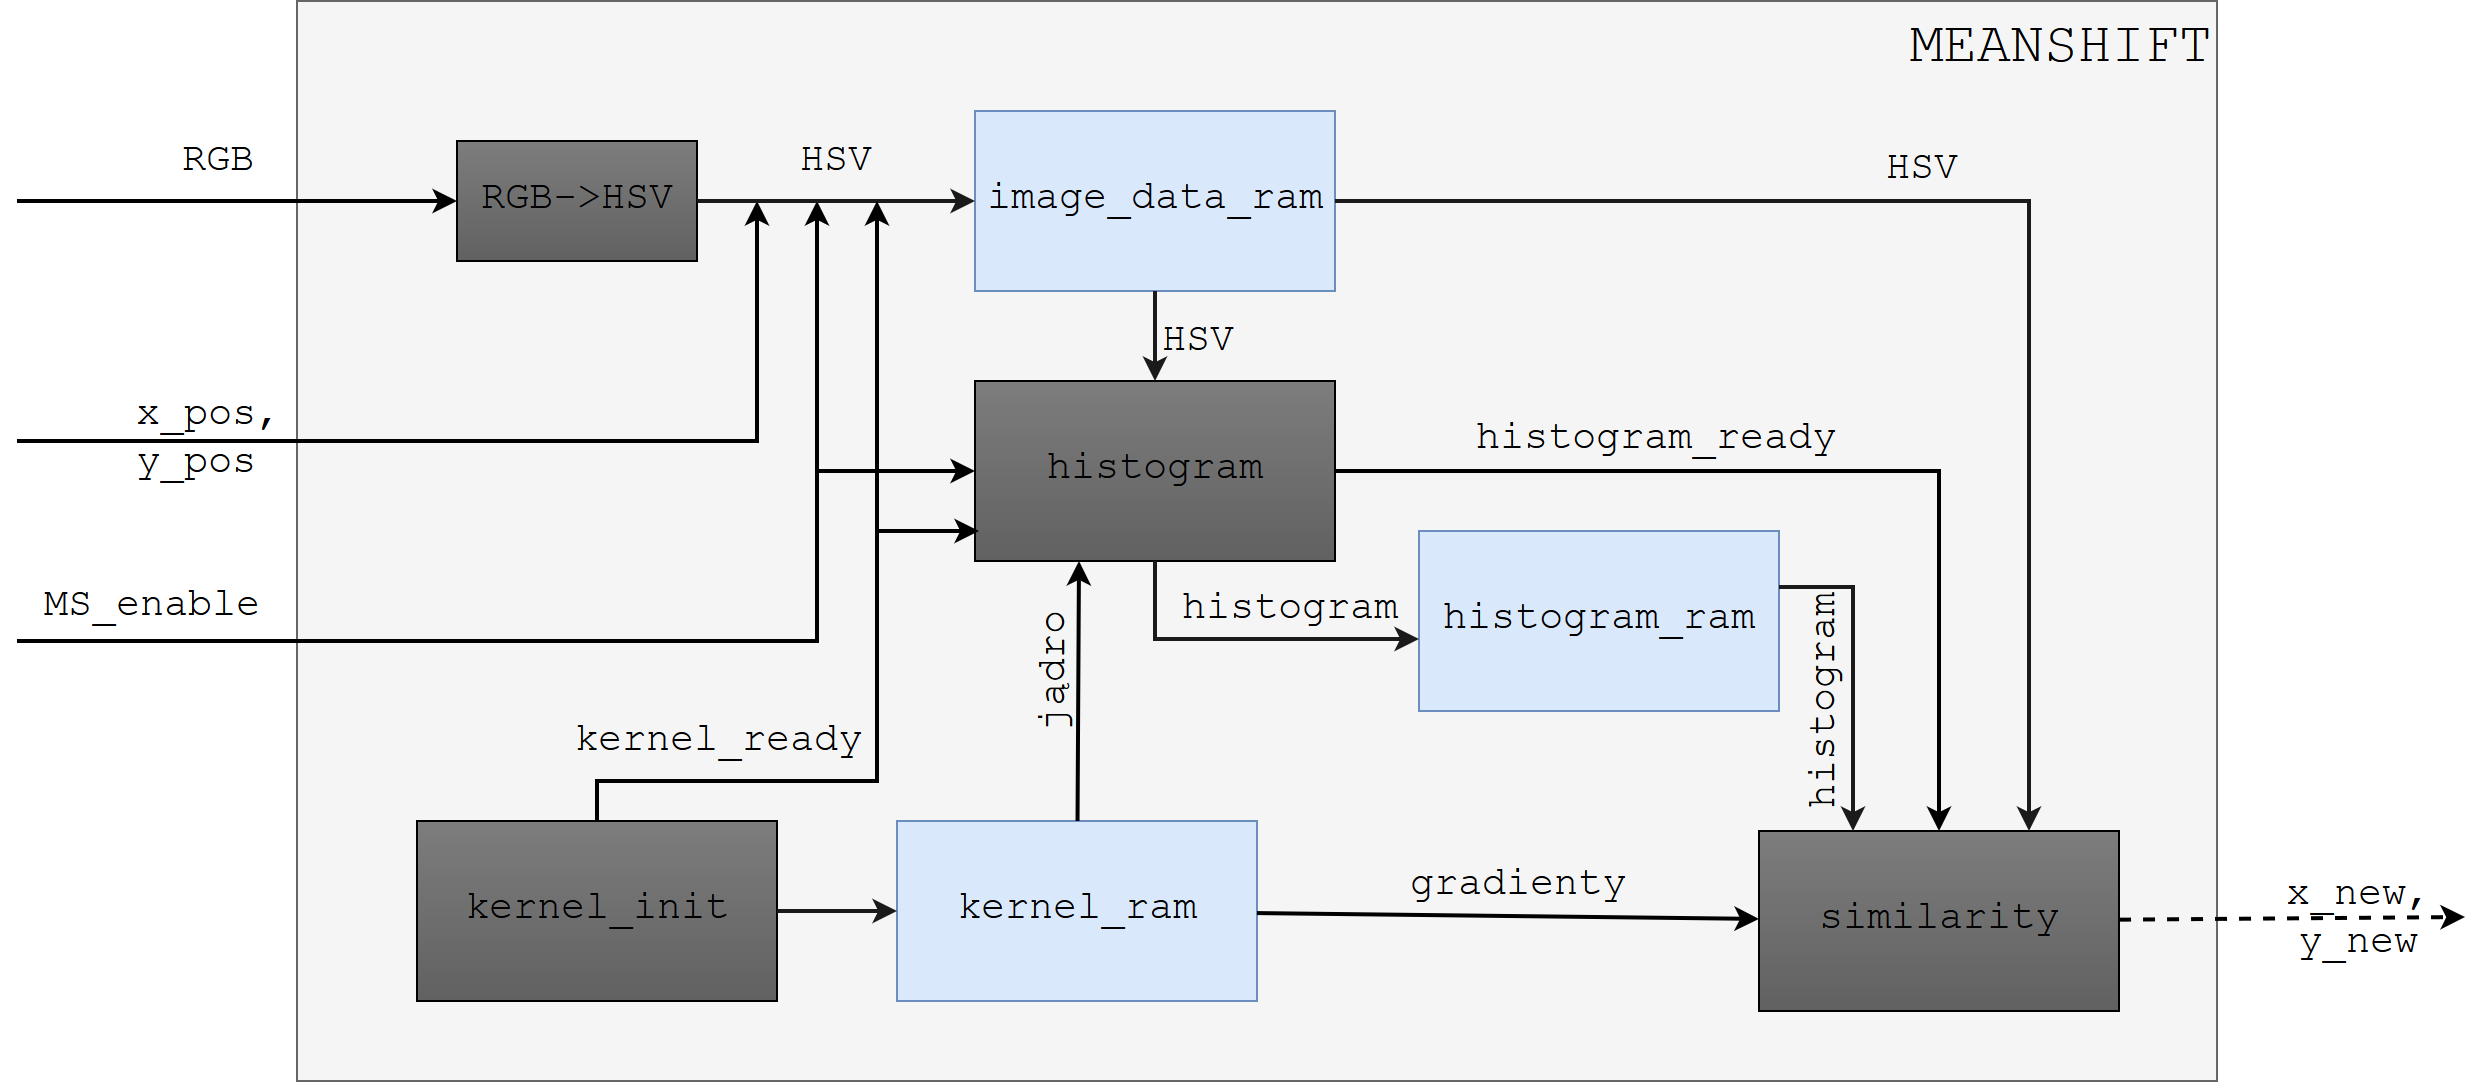
\includegraphics[width=16cm]{Meanshift.png}
	\captionsetup{justification=centering,margin=1cm}
	\caption{Schemat blokowy przedstawiający zależności pomiędzy modułami algorytmu MeanShift}
	\label{fig:MS_scheme_FPGA}
\end{figure}



\subsection{Konwersja przestrzeni barw RGB->HSV}

Wstępnym etapem toru wizyjnego wewnątrz algorytmu MeanShift jest konwersja przestrzeni barw, realizowana zgodnie ze wzorami \eqref{HSV_first}--\eqref{HSV_last} w module \textit{rgb2hsv}. 
Moduł działa w trybie potokowym pracując z~zegarem \textit{pixel\char`_clk} i odpowiednio opóźnia wszystkie sygnały sterujące, co jest istotnym warunkiem poprawnego rozpoznawania odpowiednich pikseli w dalszych etapach przetwarzania.
Dane te są na bieżąco dostarczane do modułu \textit{Meanshift}, realizującego główną część zadań. 

\subsection{Inicjalizacja}

Mimo, że właściwe działanie algorytmu ma miejsce po otrzymaniu sygnału zewnętrznego (\textit{algorithm\char`_en}), wymaga on wcześniejszej inicjalizacji -- odbywa się ona tuż po zaprogramowaniu części PL układu Zynq. 
W głównej mierze jest ona związana z obliczeniem jądra i jego gradientów. 
Dane te, wykorzystywane potem w charakterze informacji tylko do odczytu, muszą tu być zapisane w dość uporządkowany sposób. 
Najlepiej nadaje się do tego konfigurowalna pamięć BRAM. 
Powinna ona przechowywać informacje dla wszystkich elementów obszaru, to jest 10000 pól. 
Jej ostateczną organizację przedstawia tabela \ref{tab:kerBRAM}. 
W kolumnie „Format” litera \textit{U}~oznacza liczbę bez znaku, natomiast \textit{S} uwzględnia znak. Kropka oddziela dwie wartości, które określają liczbę bitów przyporządkowanych odpowiednio części całkowitej i ułamkowej (zapis stałoprzecinkowy).
\newcolumntype{P}[1]{>{\centering\arraybackslash}p{#1}}
\begin{table}[h]
\centering
\caption{Organizacja pamięci BRAM \textit{kernel\char`_ram}}
\begin{tabular}{|P{5cm} |P{3cm} |P{2.5cm}|}

\hline
\rowcolor{lightgray} Informacja & Adres rejestru & Format \\ 
Jądro: $K(||P-P'(x,y)||)$				& 0:9999		& U3.15\\ 
\hline
Gradienty: $g_x$, $g_y$		& 10000:19999	& S0.11, S0.11\\ 
\hline
Norma: $\sqrt{g_x^2+g_y^2}$	& 20000:29999	& U0.11\\ \hline
\end{tabular}

\label{tab:kerBRAM}
\end{table}


Warto nadmienić, że zestaw informacji związanych z konkretnym pikselem w obszarze 100x100 opisują rejestry pod adresami:
\begin{equation}
\{100y+x, 10000+100y+x, 20000+100y+x\}, x,y=0..99,
\end{equation}
Ułatwia to zaprogramowanie dostępu do tych danych. 
By umożliwić odczyt obydwu gradientów w jednym cyklu zegara, zagregowano je w wektor o długości rejestru, tj. 18 bitów. 
Obserwacje poczynione na zapisie gradientów w symulacji dowiodły jednak, że ich wartości są na tyle małe, że 3 najstarsze bity ułamkowe są zawsze równe bitowi znaku. 
Przykładowo, wartość $0.01$ w~formacie S0.11 ma postać $12'b111111011000$. 
Dysponując $18/2=9$ bitami na gradient można było rozszerzyć precyzję informacji pomijając te 3 nieistotne bity i zapisując ją w pamięci w notacji S0.11, a nie S0.8 -- co pozytywnie wpływa do dokładność obliczeń. 
Należy pamiętać jednak o tym, by odczyt z rejestru przechowującego gradienty dołączył te 3 bity do wartości przed rozpoczęciem jakichkolwiek obliczeń.

Pierwszym etapem inicjalizacji jest obliczenie jądra o wymiarach $100\times 100$. 
Proces ten przebiega iteracyjne, budując kolejne warstwy jądra \ref{fig:kernel} w 49 powtórzeniach (długość boku obszaru/2 -1). %TODO 2 -1 ?? %ODP (bok obszaru/2 -1) tak, w 50 iteracji byłoby dzielenie przez 0
Wartością dodawaną do odpowiednich elementów jądra jest $1/100/2=0.02$, zapisywana w formacie U3.15 jako $0.019989013671875$. 
Algorytm przechodzi przez 3 zagnieżdżone pętle, przemieszczając się po komórkach jądra \textit{\{x,y\}} i kolejnych warstwach \textit{z}. 
Schemat \ref{fig:kernel_build} przedstawia przebieg algorytmu. 
Główny warunek może wydawać się wyzwaniem, jednak wyrażenia typu $W/2$, $H/2$ wymagają jedynie przesunięcia wektora o 1 bit w prawo. 
Nie zmienia to faktu, że implementacja obliczeń wymaga uwzględnienia odpowiednich opóźnień, a~następnie synchronizacji z odczytem i zapisem danego rejestru jądra.
\begin{figure}[h]
	\centering
	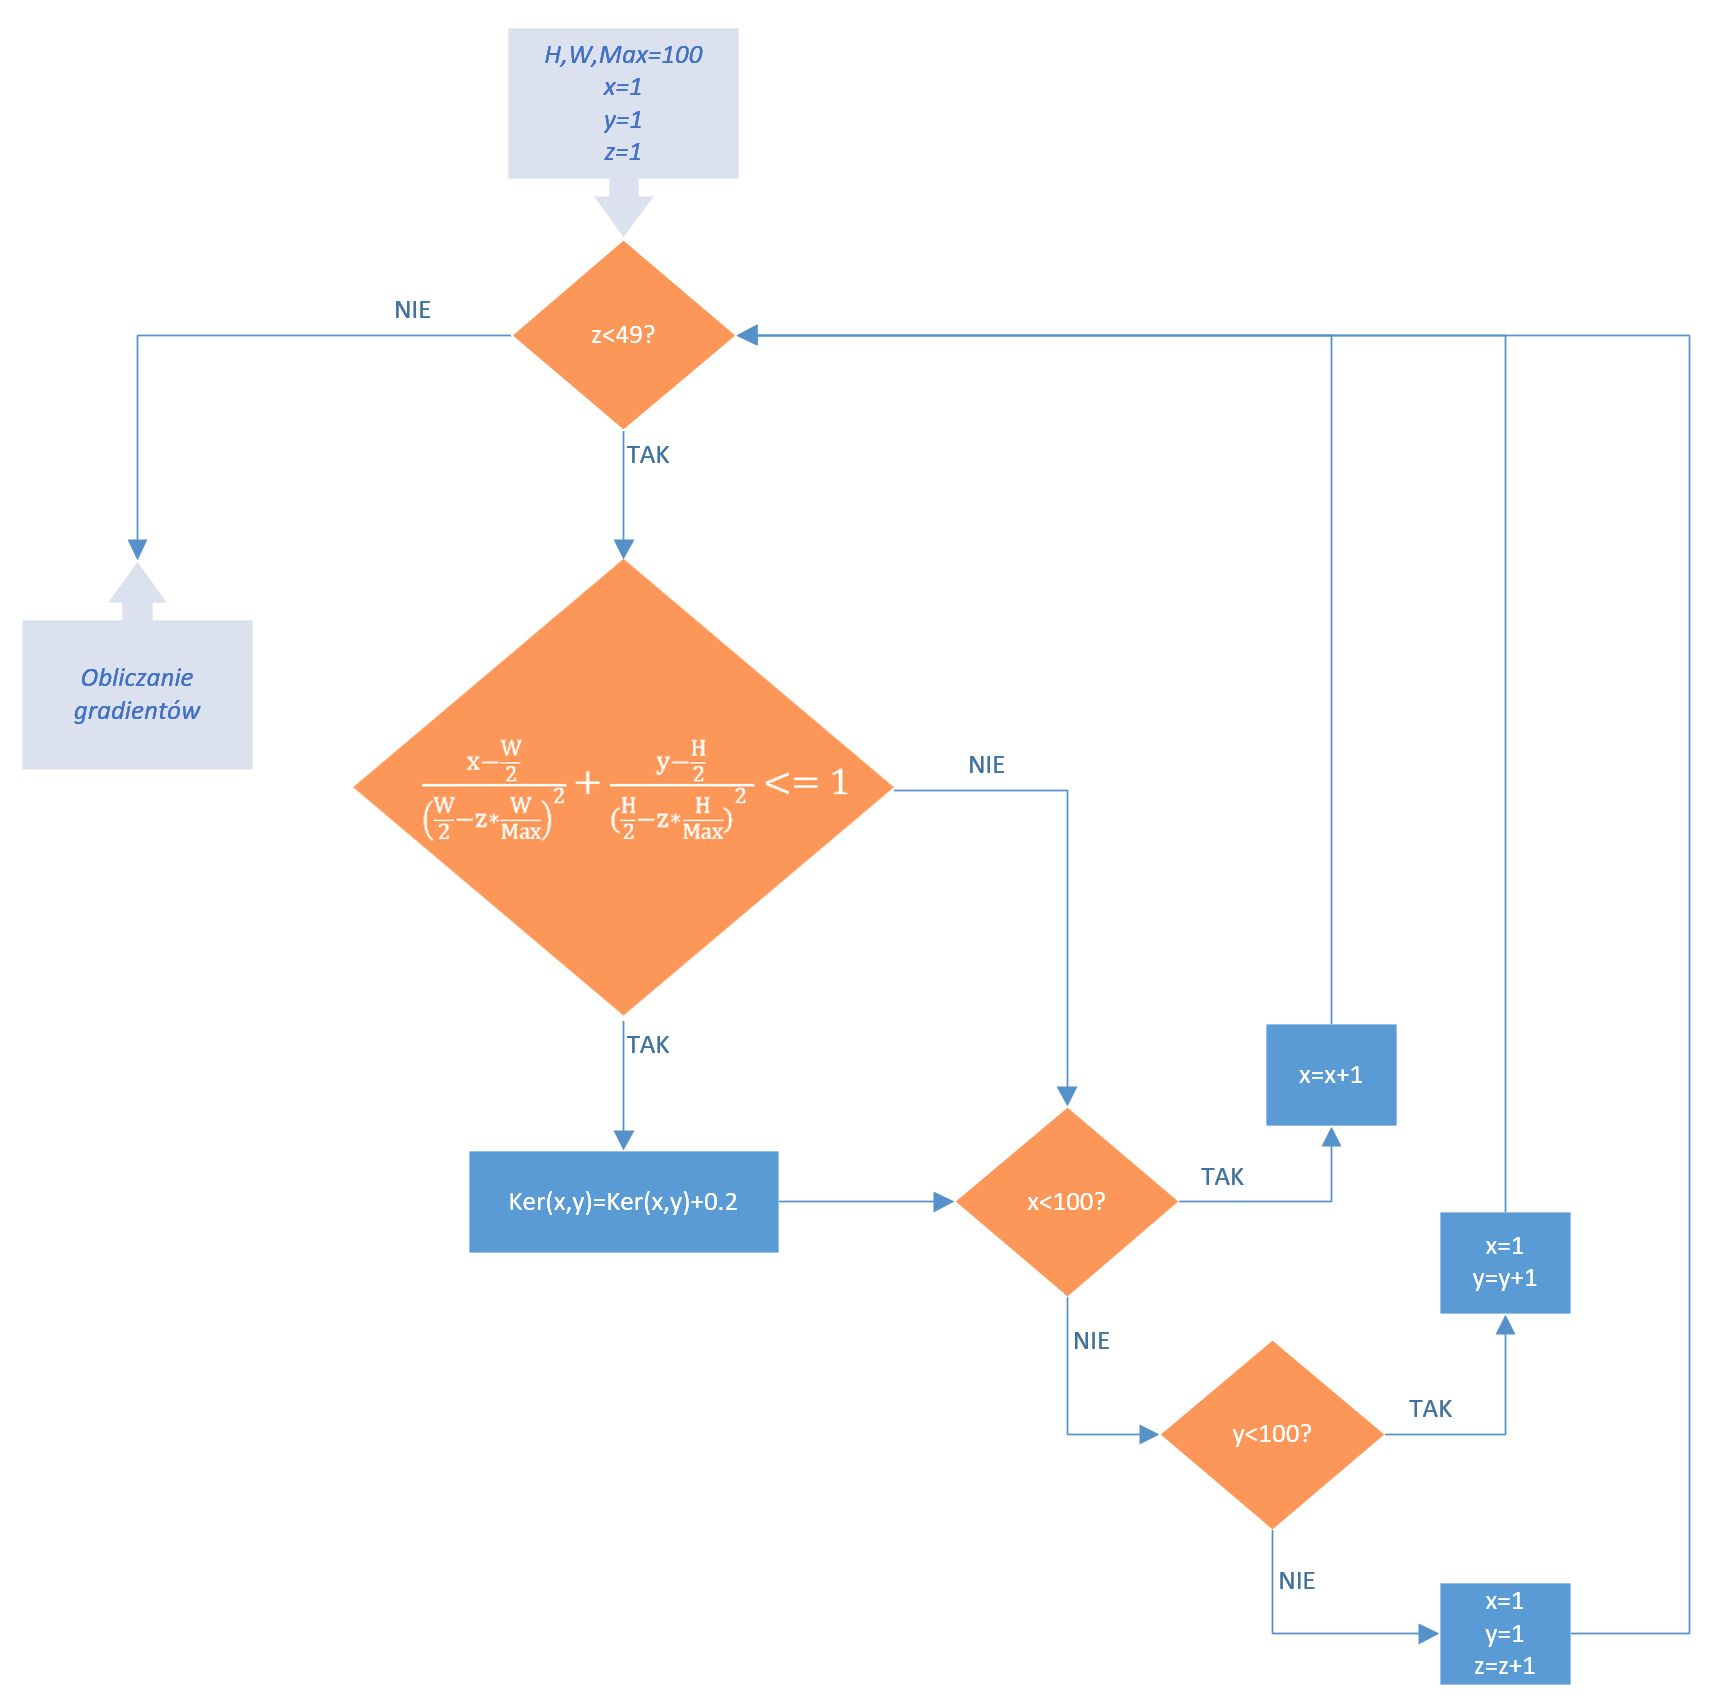
\includegraphics[width=15cm]{4_kernel.jpg}
	\caption{Proces tworzenia jądra obszaru}
	\label{fig:kernel_build}
\end{figure}

Kolejnym etapem jest obliczenie gradientów i ich normy na podstawie gotowego jądra. 
Dla każdego elementu odczytywane są wartości 4 sąsiadów i wyznaczane gradienty przy użyciu masek: $[1,0,-1]$ oraz $[1,0,-1]^T$. 
W przypadku sytuacji brzegowych niedostępny sąsiad zostaje zastąpiony rozpatrywanym elementem, a wartość gradientu jest przesuwana o jeden bit w lewo (dwukrotnie zmniejszona odległość pomiędzy obiektami skutkuje dwukrotnym powiększeniem wyniku ilorazu różnicowego). 
Na tej podstawie obliczana jest norma gradientu, która wymaga zastosowania dwóch mnożarek i pierwiastkującego bloku CORDIC. 
Jest to proces na tyle długi, że po zapisie gradientów w pamięci zdecydowano się przejść do kolejnych elementów jądra, jedynie zapamiętując adres rejestru, w którym gotowa wartość normy powinna być zapisana.

Po zebraniu kompletu danych ustawiana jest flaga \textit{kernel\char`_rom\char`_ready}, której obecność sygnalizuje gotowość uruchomienia właściwej części algorytmu. 
Jak stwierdzono w oparciu o~symulacje, w rzeczywistości inicjalizacja pamięci \textit{kernel\char`_rom} trwa około 5ms. 
Jest to zatem pomijalnie krótki czas, niewpływający na funkcjonalność (<1 klatka obrazu).


\subsection{Zapis obszaru wideo}
\label{ssec:savideo}

Na szerszy opis zasługuje sposób zapisu informacji z obrazu, należy bowiem tymczasowo zapamiętać wartości pikseli $H$, na których będą kilkukrotnie wykonywane obliczenia. 
Dużym obciążeniem dla zasobów układu byłaby próba zapisania całych klatek -- pojedyncza wymagałaby: $1280\cdot720\cdot9\text{b} = 1.037$MB dostępnego miejsca. 
Z tego względu postanowiono zapisywać jedynie obszar w aktualnym położeniu obiektu, z dodatkowym sąsiedztwem 15 pikseli z każdej strony. 
Szerokość sąsiedztwa dobrano metodą doświadczalną, uwzględniając maksymalne przemieszczenia obiektu pomiędzy kolejnymi klatkami i ograniczenia związane z zasobami.
W procesie zapisu uwzględniono zabezpieczenie na wypadek próby wyjścia poza przestrzeń obrazu. 
Opiera się ono na sprawdzeniu pozycji środka obszaru względem ramki obrazu -- minimalna odległość od każdej krawędzi to $65$. 
Zabezpieczenie to funkcjonuje również w samym algorytmie, utrzymując ostateczną pozycję obszaru wewnątrz dozwolonego wycinka ramki.

Proces śledzenia musi poprawnie określić położenie aktualnego, \enquote{użytecznego} piksela, a~także rozpoznać początek kolejnej klatki. 
Jest to możliwe poprzez stworzenie logiki opierającej się na licznikach: horyzontalnym i wertykalnym, która wykrywa zbocza sygnałów sterujących. Liczniki wykorzystują informacje przedstawione na rysunku \ref{fig:720_frame}; zliczają odpowiednio do wartości 1280 oraz 720.

Otrzymanie sygnału \textit{algorithm\char`_en} inicjuje realizację algorytmu. 
Istotne jest, aby w momencie pojawienia się tego sygnału, w obszarze zdefiniowanym jako startowy (domyślnie środek obrazu) znajdował się śledzony obiekt. 
Obszar ten, będący od teraz wzorcem, jest zatrzaskiwany na najbliższej pełnej klatce obrazu. 
Następnie obliczana jest funkcja gęstości prawdopodobieństwa, opisana w podrozdziale \ref{ssec:fgp}. 

Wartości pikseli -- linia po linii --  są przechowywane w module BRAM działającym w trybie True Dual Port, \textit{image\char`_data\char`_ram}.
Dzięki temu możliwy jest jednoczesny zapis/odczyt pod warunkiem, że porty nie pracują jednocześnie na tym samym adresie. 
Ze względu na konieczność posiadania kompletnego fragmentu obszaru i możliwość zapisu kolejnego, pamięć zdolna jest pomieścić 2 obszary z ostatnich klatek, każdy o wymiarach $130 \times 130$: łącznie 33800 adresów. 
Zamiennie, co klatkę, wykonywany jest zapis najnowszych danych do jednej połowy przestrzeni, i przetwarzanie (odczyt) drugiej \ref{tab:imageBRAM}. 

\newcolumntype{P}[1]{>{\centering\arraybackslash}p{#1}}
\begin{table}[h]
	\centering
	\caption{Organizacja pamięci BRAM \textit{image\char`_data\char`_ram}}
	\begin{tabular}{|P{4cm} |P{3cm} |P{2cm}|}
		
		\hline
		\rowcolor{lightgray} Informacja & Adres rejestru & Format \\ 
		Klatka $t\%2==0$			& 0:16899		& U9\\ 
		\hline
		Klatka $t\%2==1$		& 16900:33799	& U9\\ 
		\hline
	\end{tabular}

	\label{tab:imageBRAM}
\end{table}


%TODO Jednego nie rozumiem. Zatrzaskiwany jest też wzorzec, czy tylko są dla niego obliczany histogram.
%ODP Zatrzaskiwany jest histogram wzorca, do bieżącego śledzenia wymagane są jedynie wartości pikseli kandydata.
%TODO 2 No ale pisze Pan jednak co innego.... %ODP w sumie nie wyraziłem się jasno - zapisywany jest wzorzec, jedynie po to, żeby zapisany mógł zostać histogram. Czyli tak jak dla każdego kolejnego obszaru.

\subsection{Funkcja gęstości prawdopodobieństwa}
\label{ssec:fgp}

Wartość funkcji gęstości prawdopodobieństwa jest inaczej wartością histogramu dla danej barwy piksela ($H$ z zakresu 0-359). 
W tym celu utworzono pamięć BRAM, która przechowuje dwa histogramy dla wzorca oraz kandydata -- w sumie 720 rejestrów \ref{tab:histBRAM}. 
\newcolumntype{P}[1]{>{\centering\arraybackslash}p{#1}}
\begin{table}[h]
	\centering
	\caption{Organizacja pamięci BRAM \textit{histogram\char`_ram}}
	\begin{tabular}{|P{4cm} |P{3cm} |P{2cm}|}
		
		\hline
		\rowcolor{lightgray} Informacja & Adres rejestru & Format \\ 
		Histogram wzorca			& 0:359		& U10.15\\ 
		\hline
		Histogram kandydata		& 360:719	& U10.15\\ 
		\hline
	\end{tabular}

	\label{tab:histBRAM}
\end{table}

Histogram wzorca jest tworzony raz, w oparciu o pierwszy obraz; kolejne histogramy są związane z kandydatem i zostają zapisane w górnej połowie adresowej ($H+360$). 
Wartość piksela, umożliwiając dostęp do odpowiedniego rejestru pamięci, pozwala na odczyt dotychczasowej wartości przedziału histogramu i przygotowanie go do aktualizacji. 
Z kolei współrzędne piksela w odniesieniu do obszaru $100 \times 100$ są wykorzystywane do odczytu elementu jądra. 
Przedział histogramu jest aktualizowany zapisem sumy obu wartości. 
Wielkość rejestrów pamięci \textit{histogram\char`_ram} pozwala na zapis wartości w formacie U10.15, czyli w zakresie [0:1023.99997]. %TODO 2 format w formacie ? %DOP OK
Zdarzają się jednak przypadki, gdy większość pikseli na obszarze (zwłaszcza w centrum -- miejscu największych wartości jądra) jest jednokolorowa, co może skutkować przekroczeniem dopuszczalnych wartości dla rejestru. 
Chroni przed tym dodatkowy fragment logiki, który wykrywając takie zdarzenie, pozostawia rejestr z maksymalną wartością.

Wartość pikseli jest odczytywana bezpośrednio z pamięci przechowującej analizowany obszar  (opisanej w podrozdziale \ref{ssec:savideo}). 
Do obliczenia histogramu wymaganych jest jedynie $100\times 100$ pikseli, pozostałe (sąsiedztwo) należy zignorować. 
Wartości \textit{offset\char`_X} oraz \textit{offset\char`_Y} określają pozycję pierwszego analizowanego piksela (w lewym górnym rogu). 
Startując z tego miejsca, praca liczników \textit{H\char`_count} oraz \textit{W\char`_count} pomaga w zebraniu jedynie 100 pikseli ze 100 linii. 
Przykładowo, obliczając po raz pierwszy histogram dla ostatnio zapisanej klatki zmienne \textit{offset\char`_X} i \textit{offset\char`_Y} mają wartości domyślne $(15,15)$. 
Oznacza to, że z zapisanego obszaru o~wymiarach $130\times 130$ należy odczytać jego środek, a~współrzędne pierwszego piksela będą wynosić $(15,15)$. 
W kolejnych iteracjach algorytmu, dla tej samej klatki obrazu, zmienne mogą przyjąć inne wartości, tworząc w efekcie funkcję gęstości prawdopodobieństwa odpowiadającą nowemu fragmentowi obszaru $100\times 100$. 
Zakres dopuszczalnych wartości dla każdej z tych zmiennych to $<0,29>$. 

Po przejściu przez wszystkie piksele obszaru następuje ustawienie flagi \textit{histogram\char`_ready}, gdzie w przypadku przetwarzania klatki-wzorca kolejnym zadaniem jest akwizycja pierwszego kandydata, natomiast dla każdej kolejnej rozpocznie obliczanie funkcji podobieństwa.
Podobnie jak \textit{image\char`_data\char`_ram}, \textit{histogram\char`_ram} działa w trybie True Dual Port. 
Po obliczeniu funkcji gęstości dla aktualnego obszaru, z pamięci jednocześnie są odczytywane wartości funkcji dla wzorca (port A) i kandydata (port B pamięci) -- umożliwiając wykonywanie części dalszych obliczeń w sposób równoległy. 

\subsection{Funkcja podobieństwa}

Moduł implementujący obliczanie funkcji podobieństwa (i ostatecznie przesunięcia) obszaru, jest najbardziej złożony w tej części systemu. 
Funkcja podobieństwa, opisana wzorem \eqref{eq:position}, jest wyznaczana dla każdego piksela w pamięci, należącym do właściwego obszaru (bez sąsiedztwa). 

Dla każdego piksela z obszaru $100 \times 100$, którego wartość $H$ jest adresem dla pamięci $histogram\char`_ram$, wczytywana jest wartość funkcji prawdopodobieństwa wzorca i kandydata. 
Moduł oblicza ich iloraz (wzorzec/kandydat) używając bloku Divider Generator (w wersji 5.1) dostarczonego przez firmę Xilinx.
Ze względów optymalizacyjnych obcięto 9 najmłodszych bitów obu wartości, gdyż nie wpływały w większym stopniu na dokładność, a ich pominięcie pozwoliło zmniejszyć latencję modułu.
Podczas takiego dzielenia logika musi ponadto sprawdzić obecność zera w mianowniku -- wówczas iloraz powinien być zerowany. 
Brak obsługi takiego zdarzenia doprowadziłby do otrzymania ilorazu o trudnej do przewidzenia wartości -- mogłoby to powodować poważne błędy w działaniu algorytmu. 

Gotowy iloraz należy poddać pierwiastkowaniu. 
Moduł obliczający pierwiastek wymaga, by wejście z danymi było liczbą całkowitą lub  też ułamkową -- ale z jednym bitem dla części całkowitej: U1.X. 
W tym celu wynik dzielenia -- liczba w formacie: U16.16 -- została obcięta do U13.11., a następnie ,,wirtualnie'' przesunięta o 12 bitów w prawo, do postaci: U1.23. 
Wynik pierwiastkowania wymaga przesunięcia w lewo już tylko o 6 bitów ($\sqrt{2^{12}}=2^6$), po czym jest obcinany do 16 najbardziej znaczących bitów: U7.9.
Operacje te, mimo że zawiłe, nie wpływają na wynik, lecz gwarantują poprawne działanie modułu \textit{CORDIC} realizującego pierwiastkowanie.

Wartości pierwiastka współtworzyć będą zarówno licznik, jak i mianownik ilorazu wektora MeanShift -- oddzielnie dla przesunięcia pionowego i poziomego.
Obliczenie iloczynów wymaga pobrania z pamięci \textit{kernel\char`_ram} obu gradientów oraz ich normy. 
Logika realizująca odczyt jest zoptymalizowana pod zminimalizowanie liczby cykli zegara potrzebnych na dostęp do obu wartości i została oparta o maszynę stanu. %TODO 2 odczyt, odczytania... powt. %ODP OK
Po zakończeniu przetwarzania wszystkich pikseli obszaru $100 \times 100$ (sumowania obliczonych na ich podstawie wartości) ustawiana jest flaga \textit{div\_enable\_de}, która jest podłączona do modułów realizujących dzielenie w wektorze MeanShift. 
Otrzymane wyniki dzielenia odpowiadają przesunięciu obszaru śledzenia, należy je jednak znormalizować do postaci całkowitej i upewnić się, że obszar po przesunięciu nadal będzie w całości znajdował się w zapisanym fragmencie o wymiarach $130 \times 130$. 
Pozwoli to wykonać kolejne iteracje, które mogą poprawić wynik śledzenia. 
O ile pierwsza iteracja rozpoczyna analizę w środku obszaru, to w trakcie kolejnych informacja o położeniu obszaru wewnątrz $130 \times 130$ jest zapamiętywana przez zmienne \textit{offset\_X} oraz \textit{offset\_Y}.


\section{Realizacja algorytmu HOG+SVM}
\label{HOG_SVM_realization}
Wymagania stawiane przez system mówią o konieczności rozpoznania osoby wraz z dodatkowym określeniem jej wielkości na ekranie (skala ta pozwoli dość zgrubnie wyznaczyć odległość drona od obiektu, co wpłynie na sterowanie maszyny). 
Jednym z celów jest bowiem utrzymanie stałej odległości od postaci.
Z tego względu implementacja musi wykorzystać tzw. piramidę skal, czyli równoległą detekcję HOG+SVM na serii obrazów o różnych wymiarach.
Dysponując obrazem o rozdzielczości $1280 \times720$, należy przeskalować go do kilku mniejszych, a następnie przeprowadzić na nich opisane wcześniej operacje wyliczenia wektora cech i sklasyfikować go przy użyciu SVM. 
Odpowiednia lokalizacja postaci (i jej odległość od kamery) zostanie wybrana na podstawie najlepszego \textbf{pozytywnego} wyniku klasyfikacji, w oparciu o~wartość $r$ \eqref{eq:HOG_classification} (pełny opis algorytmu znajduje się w podrozdziale \ref{sec:HOG&SVM}).
%TODO 2 jeszcze ref do opisu algortmu... %ODP OK

Algorytm ten może rozpocząć działanie jedynie na pełnej klatce obrazu, zatem stworzono mechanizm, który niezależnie od momentu pojawienia się sygnału wyzwalającego pracę algorytmu będzie oczekiwał na zbocze opadające sygnału synchronizacji pionowej, czyli nową, pełną ramkę. 
Tylko w takim przypadku gwarantowane jest poprawne działanie metody.
Drugim warunkiem jest to, by w momencie nadejścia nowej klatki algorytm nie był w trakcie przetwarzania poprzedniej -- w przeciwnym wypadku histogramy mogłyby być nadpisywane nowymi wartościami. 
Oznacza to jednak, że co druga klatka obrazu będzie pomijana w przetwarzaniu, ograniczając częstotliwość pracy algorytmu do \textit{30Hz}.

W pierwszej kolejności obraz wejściowy poddawany jest konwersji do skali odcieni szarości. 
Następna w kolei, operacja skalowania do 5 mniejszych obrazów metodą najbliższego sąsiedztwa, jest realizowana potokowo, dzięki czemu można zachować sygnały kontrolne VGA (synchronizację poziomą oraz pionową).
Na pomniejszonych obrazach obliczane są wektory cech, bazując na komórkach o wielkości $4\times 4$ i blokach o rozmiarze $2\times2$. 
Dysponując określoną liczbą zasobów układu XC7Z020, nie jest możliwa analiza całego obrazu, a jedynie otoczenia aktualnie śledzonego fragmentu.
Musi on być jednak wystarczająco duży, by możliwe było osiągnięcie jak najlepszego wyniku detekcji osoby w jego wnętrzu. %TODO 2 średni styl. %ODP OK
Jak wspomniano wcześniej, wektor cech tworzony jest na wycinku o rozmiarze $128\times 64$ pikseli. 
Przedstawia to obraz \ref{fig:HOG_mesh}, gdzie taki wycinek zaznaczono zieloną linią. 

\begin{figure}[h]
	\centering
	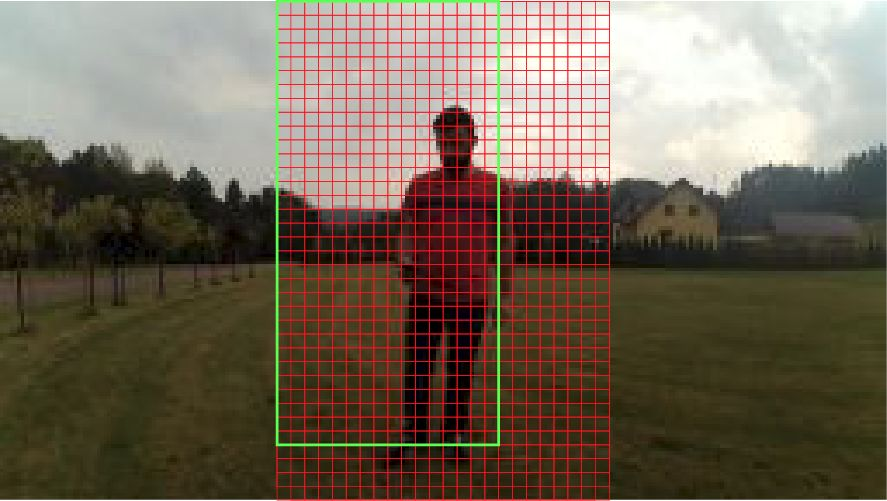
\includegraphics[width=11cm]{4_scaled_hog_example.jpg}
	\caption{Analiza obrazu o rozmiarach $144\times 256$}
	\label{fig:HOG_mesh}
\end{figure}
%\newline

Jeśli algorytm będzie pracował na obszarze $144\times 96$, to zakładając stałe położenie komórek na obrazie (są to kwadraty $4\times4$ wydzielone czerwonymi liniami), powstanie łącznie $5\cdot9=45$ wektorów cech. 
Reszta obrazu zostaje zignorowana. 
Współrzędne centrum obszaru detekcji są określane na początku działania pojedynczej iteracji algorytmu i są natychmiastowo konwertowane do odpowiednich skal obrazu. Po zakończeniu klasyfikacji współrzędne odpowiadające najlepszej detekcji są konwertowane do oryginalnej skali i wykorzystywane podczas analizy kolejnej dostępnej klatki obrazu. Rysunek \ref{fig:HOG_SVM_scheme_scaling} opisuje metodę z perspektywy działania na kilku skalach.

Ogólny schemat blokowy jest przedstawiony na rysunku \ref{fig:HOG_SVM_scheme}.  Opis poszczególnych modułów znajduje się w kolejnych podrozdziałach. %TODO 2 napiasać, że omówienie modułów w kolejnych podrozdziałach. Druga sprawa to czarne napisy na ciemnoszarym tle... no jakby to ująć - słabo to widać.... %ODP OK poprawiono

\begin{figure}[h]
	\centering
	\captionsetup{justification=centering,margin=1cm}
	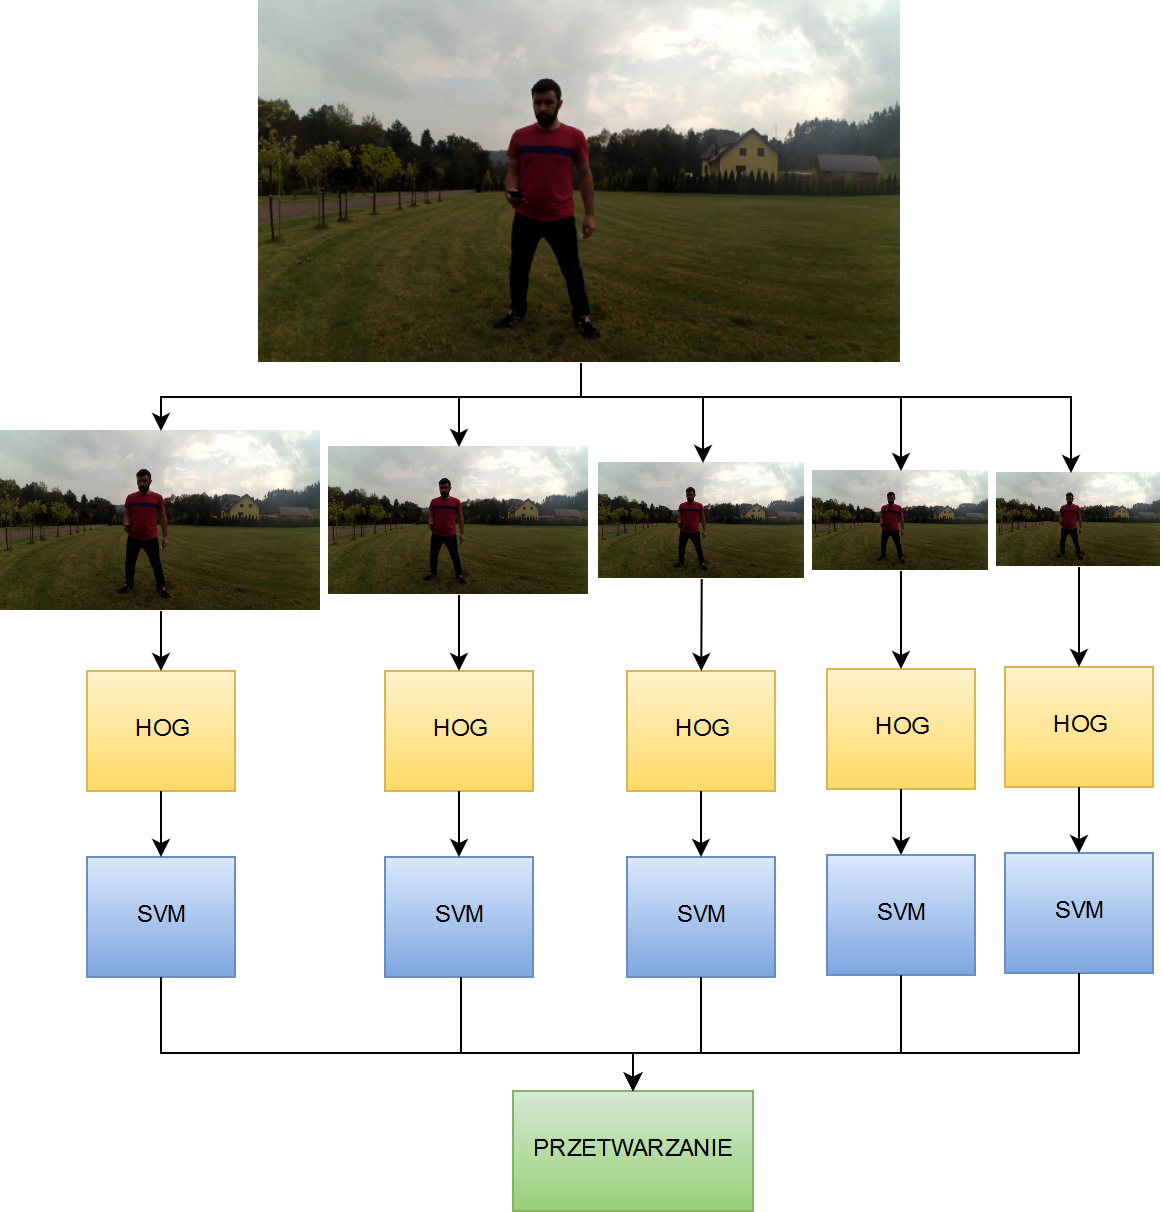
\includegraphics[width=11cm]{Scaling.png}
	\caption{Schemat przedstawiający ideę działania algorytmu HOG+SVM w wielu skalach}
	\label{fig:HOG_SVM_scheme_scaling}
\end{figure}

\begin{figure}[h]
	\centering
	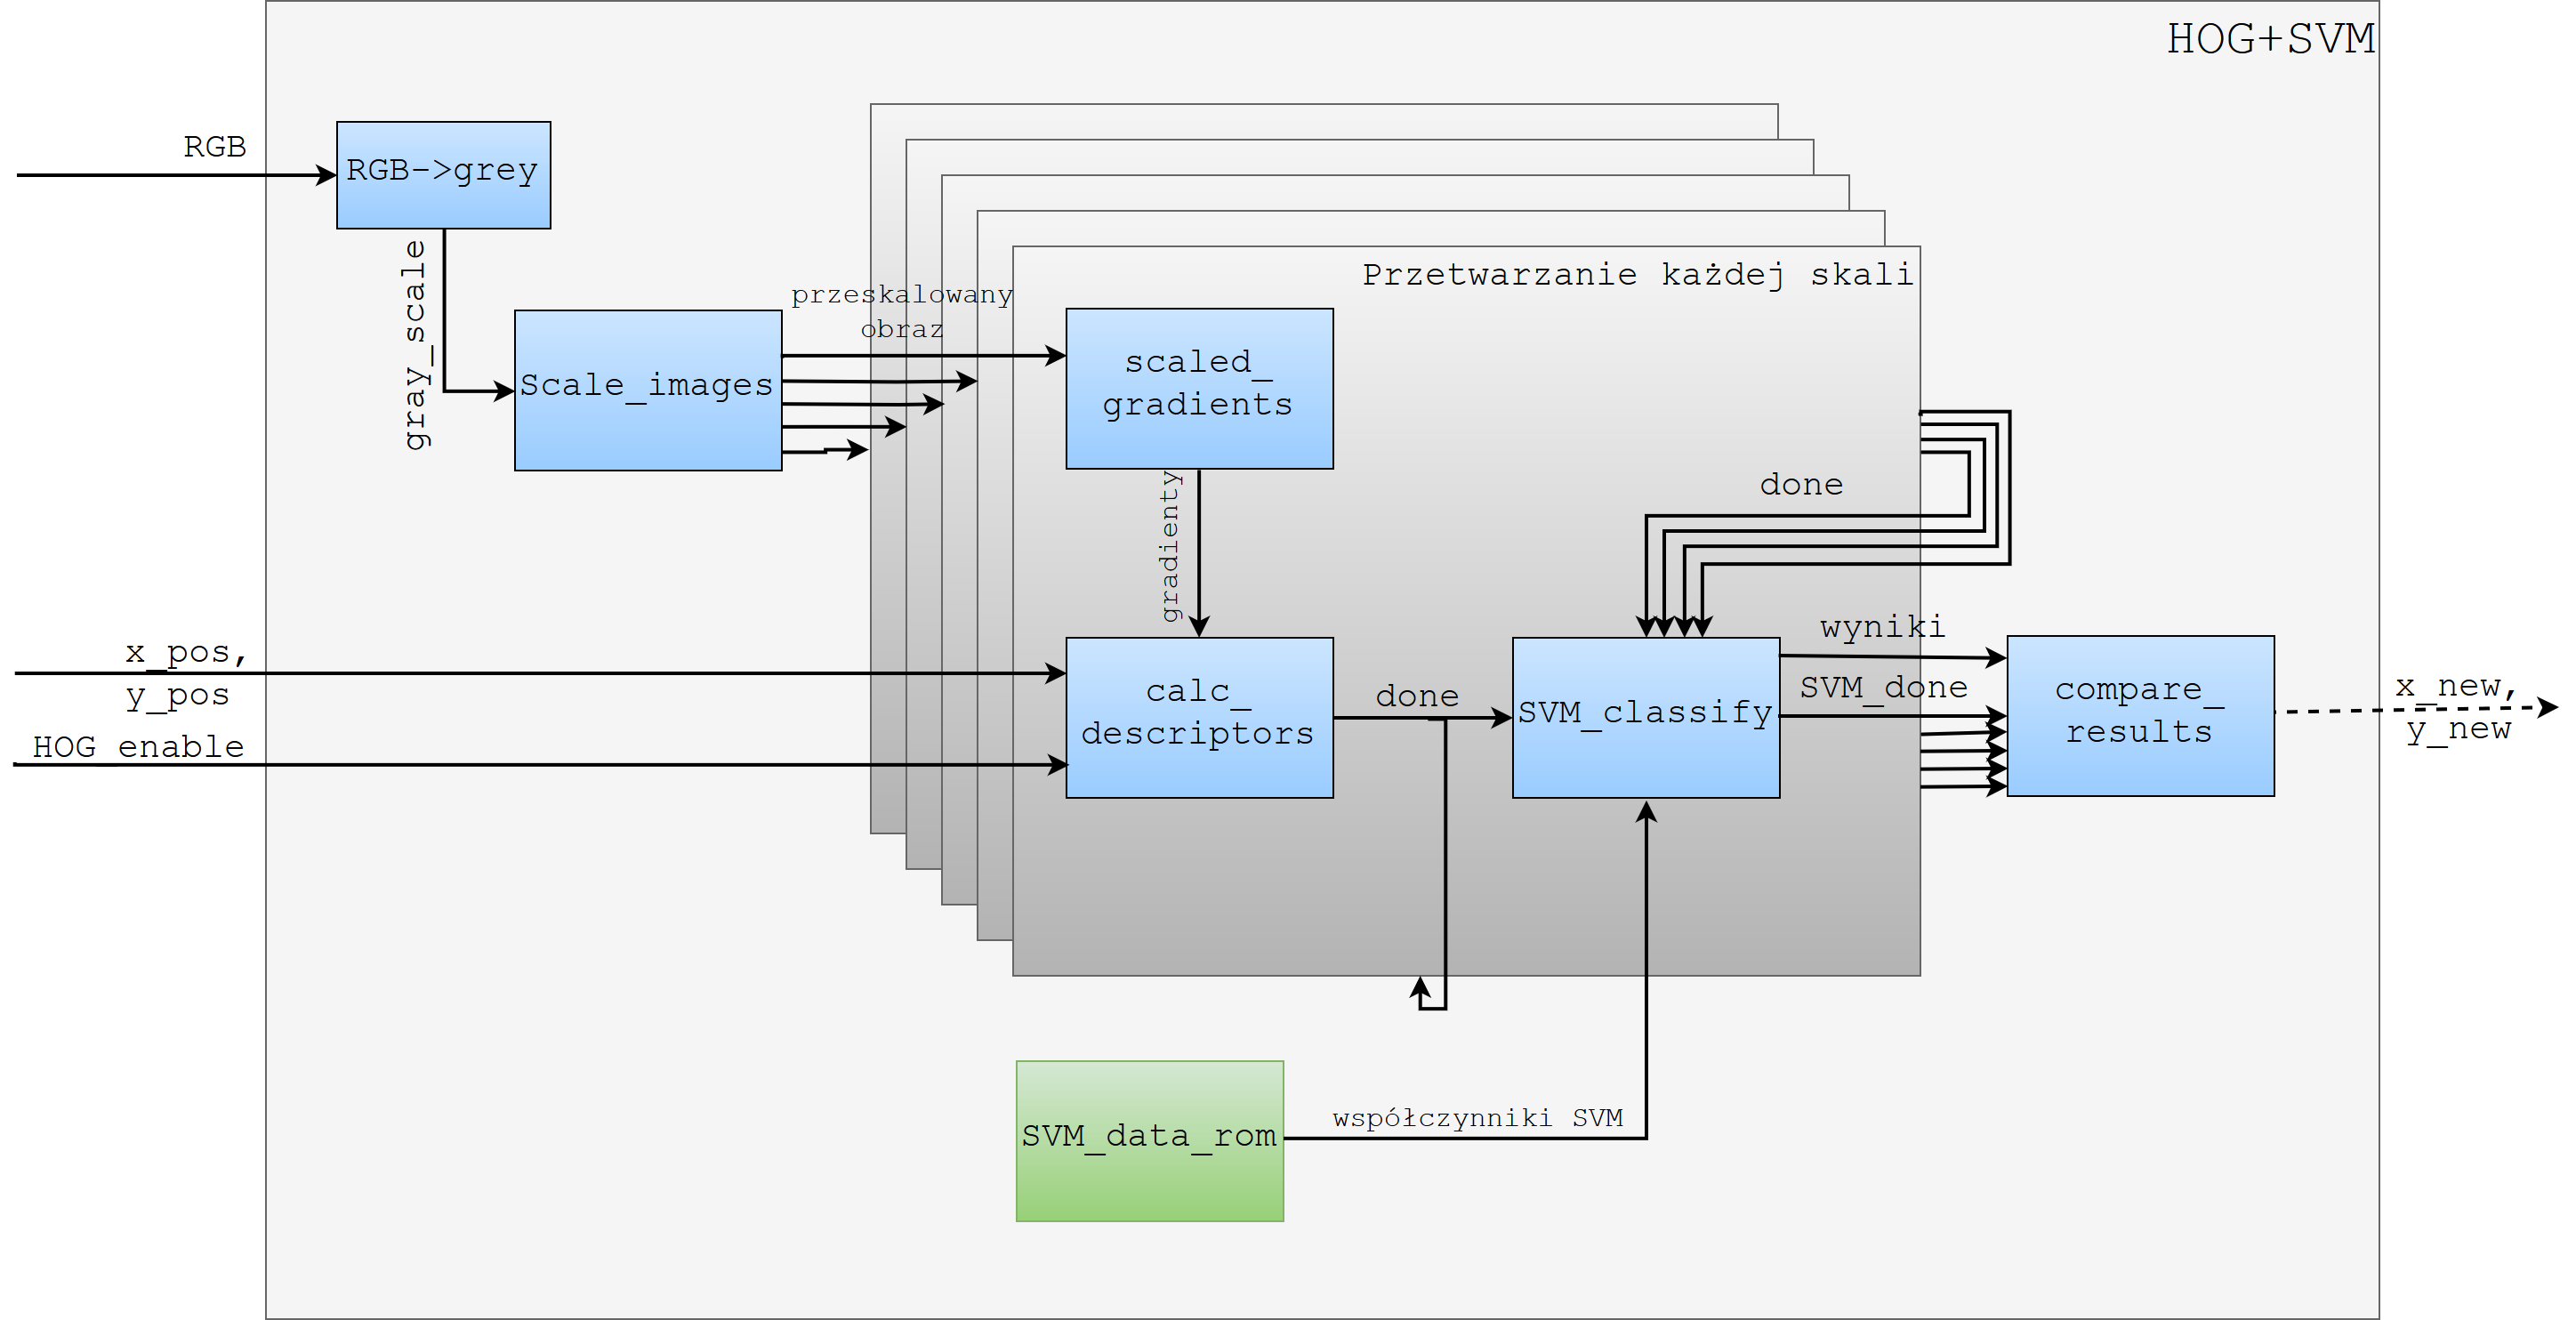
\includegraphics[width=16cm]{HOG_SVM.png}
	\captionsetup{justification=centering,margin=1cm}
	\caption{Schemat blokowy przedstawiający zależności pomiędzy modułami algorytmu HOG+SVM}
	\label{fig:HOG_SVM_scheme}
\end{figure}

\subsection{Konwersja RGB do skali odcieni szarości}

Obraz wejściowy jest poddawany konwersji zgodnie ze wzorem \eqref{eq:rgb2gray}. 
Używane są tu trzy równoległe mnożarki, a suma iloczynów jest zaokrąglana do 8 bitów (do postaci liczby całkowitej z zakresu 0-255).

\subsection{Skalowanie}

Kolejny etap to przeskalowanie obrazu wejściowego. 
Sama idea okazuje się być tym bardziej na miejscu, jeśli wziąć pod uwagę parametry kamery zamontowanej na dronie -- w przypadku tego projektu jest to Xiaomi Yi, urządzenie do zastosowań sportowych i charakteryzujące się dużym kątem widzenia -- 155$^{\circ}$.
W efekcie osoba oddalająca się od kamery bardzo szybko zmniejszy swoje wymiary na obrazie. 
Materiał $1280\times 720$ pikseli przeskalowano do 5 obrazów przy użyciu następujących skal:
\NumTabs{15}
\begin{itemize}
	\item \textbf{1:  2}\tab{:}\tab{$720\times 1280\rightarrow360\times 640$} pikseli
	\item \textbf{1:2.5}\tab{:}\tab{$720\times 1280\rightarrow288\times 512$} pikseli	
	\item \textbf{1:  3}\tab{:}\tab{$720\times 1280\rightarrow240\times 426$} pikseli
	\item \textbf{1:3.5}\tab{:}\tab{$720\times 1280\rightarrow205\times 365$} pikseli
	\item \textbf{1:  4}\tab{:}\tab{$720\times 1280\rightarrow180\times 320$} pikseli
\end{itemize}

Powyższe wartości pozwalają jednocześnie zachować prostotę implementacji (skale są reprezentowane w formacie U3.1) i z akceptowalnym marginesem błędu określić odległość drona od postaci.
Skalowanie przebiega w dość prosty sposób i polega na pomijaniu odpowiednich wierszy lub/i kolumn oryginalnego obrazu. 
Jeśli założyć, że: 
\begin{itemize}
	\item $x_i$, $y_i$ -- współrzędne obrazu wejściowego,
	\item $x_o$, $y_o$ -- współrzędne obrazu wyjściowego (przeskalowanego),
	\item $s_c$ -- skala do zastosowania w pionie oraz w poziomie,
\end{itemize}
to przypisanie wartości obrazu wejściowego nastąpi przy jednoczesnym spełnieniu obu poniższych warunków:
\begin{equation}
\label{eq:scaling}
\left.\begin{aligned} 
x_i&==\lfloor s_cx_o\rfloor \\ 
y_i&==\lfloor s_cy_o \rfloor
\end{aligned}\right.
\end{equation}
Po natrafieniu na odpowiedni piksel, oprócz przypisania jego wartości do wyjścia, wystawiony zostanie sygnał sterujący \textit{valid}, bardzo ważny dla dalszej części algorytmu.
Przykład dla kilku pierwszych wartości \textit{x\char`_o} jest widoczny w tabeli \ref{tab:scaling}.
\begin{table}[h]
	\centering
	\captionsetup{justification=centering,margin=1cm}
	\caption{Przykładowy przebieg skalowania dla $s_c=2.5$ wraz z przypisywanymi pikselami wejściowymi}	
	\begin{tabular}{|P{2cm} |P{3cm} |P{2cm}|}	
		\hline
		\rowcolor{lightgray} $x_o$ & $x_is_c$ & $x_i$ \\ 
		1		& 2.5	& 2\\ 
		\hline
		2		& 5		& 5\\ 
		\hline
		3		& 7.5	& 7\\ 
		\hline
		4		& 10	& 10\\ 
		\hline		
	\end{tabular}
	\label{tab:scaling}
\end{table}

Działanie modułu opiera się na stworzeniu dwóch zestawów liczników dla każdej skali. 
Pierwszy zestaw pozwala na określenie indeksów piksela wejściowego ($x_i$, $y_i$) i został opisany w rozdziale \ref{sec:counter}. 
Drugi zestaw liczników działa zgodnie ze schematem \ref{fig:scaling_sch}.
Oznaczeniem \mbox{\textit{@PixelClk}} opisano proces oczekiwania na kolejne zbocze narastające zegara piksela. 
W~momencie pojawienia się sygnału synchronizacji pionowej następuje inicjalizacja liczników współrzędnymi piksela zlokalizowanego w lewym górnym rogu docelowej klatki skalowanego obrazu. 
W trakcie otrzymywania kolejnych pikseli na wejściu porównywane są wartości obu liczników -- spełniony warunek oznacza wystawienie wartości piksela na wyjście modułu wraz z sygnałem aktywnym. 
W przeciwnym wypadku sygnał aktywny jest wystawiany w~stan nieaktywny. 
Obecna na schemacie zmienna \textit{flag} służy do jednorazowych inkrementacji licznika $y_0$~z~uwagi na dwie kwestie:
\begin{itemize}
	\item sygnał synchronizacji poziomej jest ustawiany na 40 cykli zegara pikselowego,
	\item sygnał synchronizacji poziomej jest obecny po sygnale synchronizacji pionowej, a przed nadejściem pierwszego piksela.
\end{itemize}   
\begin{figure}[!h]
	\centering
	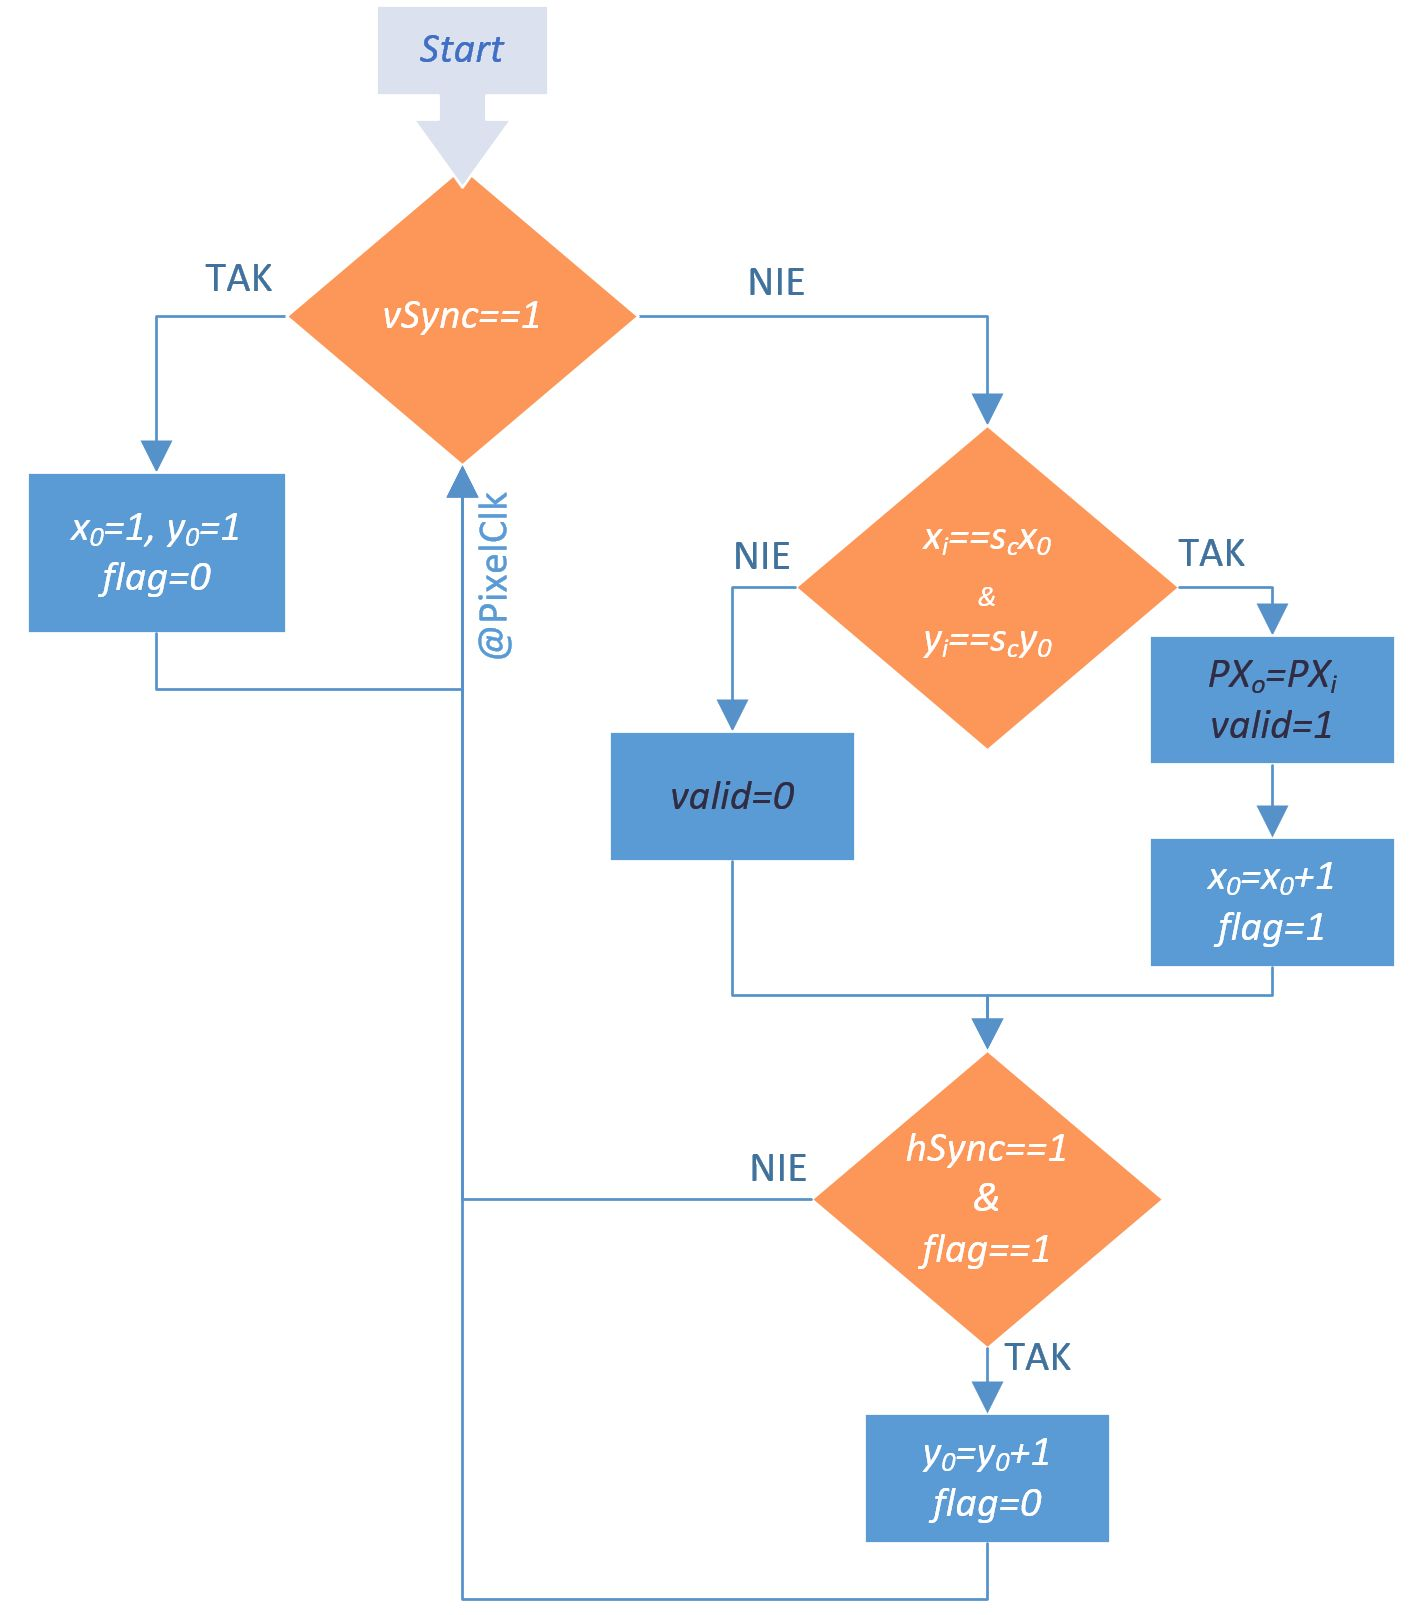
\includegraphics[width=11cm]{4_scaling.jpg}
	\caption{Schemat działania licznika skalującego}
	\label{fig:scaling_sch}
\end{figure}


Gwarancją poprawnie przeprowadzonego procesu skalowania jest obecność sygnałów sterujących VGA -- tylko wtedy następuje poprawny przyrost wartości liczników. 
Z kolei inicjalizacja (po lewej stronie diagramu) ma miejsce po otrzymaniu sygnału synchronizacji pionowej, zatem podłączony do układu sygnał wideo będzie skalowany już od pierwszej pełnej klatki.

%TODO albo tu albo wcześniej jest potrzebny schemat jak to wygląda - może ogólny. Że jest ramka wejściowa. 5 wynikowych potem HOG i klasyfikacja.
%TODO 2 -> na początku tej czesci o HOG - taki poglądaowy 10 min paint. %ODP OK

\subsection{Obliczanie gradientów}

Odpowiednio przeskalowane obrazy są zbyt duże, by przechowywać informację o ich gradientach w wewnętrznych zasobach układu XC7Z020. Do ich obliczenia zastosowano moduł działający potokowo i opierający działanie o sygnał aktywnego piksela \textit{valid} z modułu skalowania. 
%TODO 2 to bym usunął i po prostu napisał, że Do obliczania gradientów zastosowano moduł działający potokowo - czy coś takiego. %ODP OK

Implementacja gradientu pionowego jest nieco złożona, gdyż wymagane w pojedynczej operacji piksele leżą w kilku kolejnych liniach obrazu. 
Konieczne jest zapamiętanie dwóch ostatnich linii -- zrealizowano to przy użyciu dwóch kolejek FIFO \ref{fig:fifo_gradient}.
Do jednej z nich (oznaczonej numerem \#1) wpisywane są wartości bieżących pikseli.
Przejście do każdej kolejnej linii obrazu powoduje systematyczną wymianę pikseli na najnowsze - wówczas do kolejki \#2~są zapisywane wartości bezpośrednio z \#1.
Logika została zaprojektowana w sposób pozwalający uzyskać jednoczesny dostęp do 3 kolejnych pikseli leżących w linii pionowej. 
Umożliwia to specjalny tryb modułu FIFO -- First Word Fall Through (FWFT), dzięki któremu pierwsze dostępne słowo jest natychmiastowo wystawiane na wyjście, i tylko zdejmowane (zastępowane kolejnym) w odpowiedzi na wysoki stan sygnału odczytu \cite{FIFO}. %TODO nie duża załuga, tylko umożliwia to %ODP OK
Ostatecznie logika, będąc w~linii $i$ ($i>1$), obliczy gradient pionowy dla piksela z linii $i-1$. %TODO nie poniżej tylko \ref. no i nie algorytm %ODP OK, \ref umieszczono wyżej
\begin{figure}[h]
	\centering
	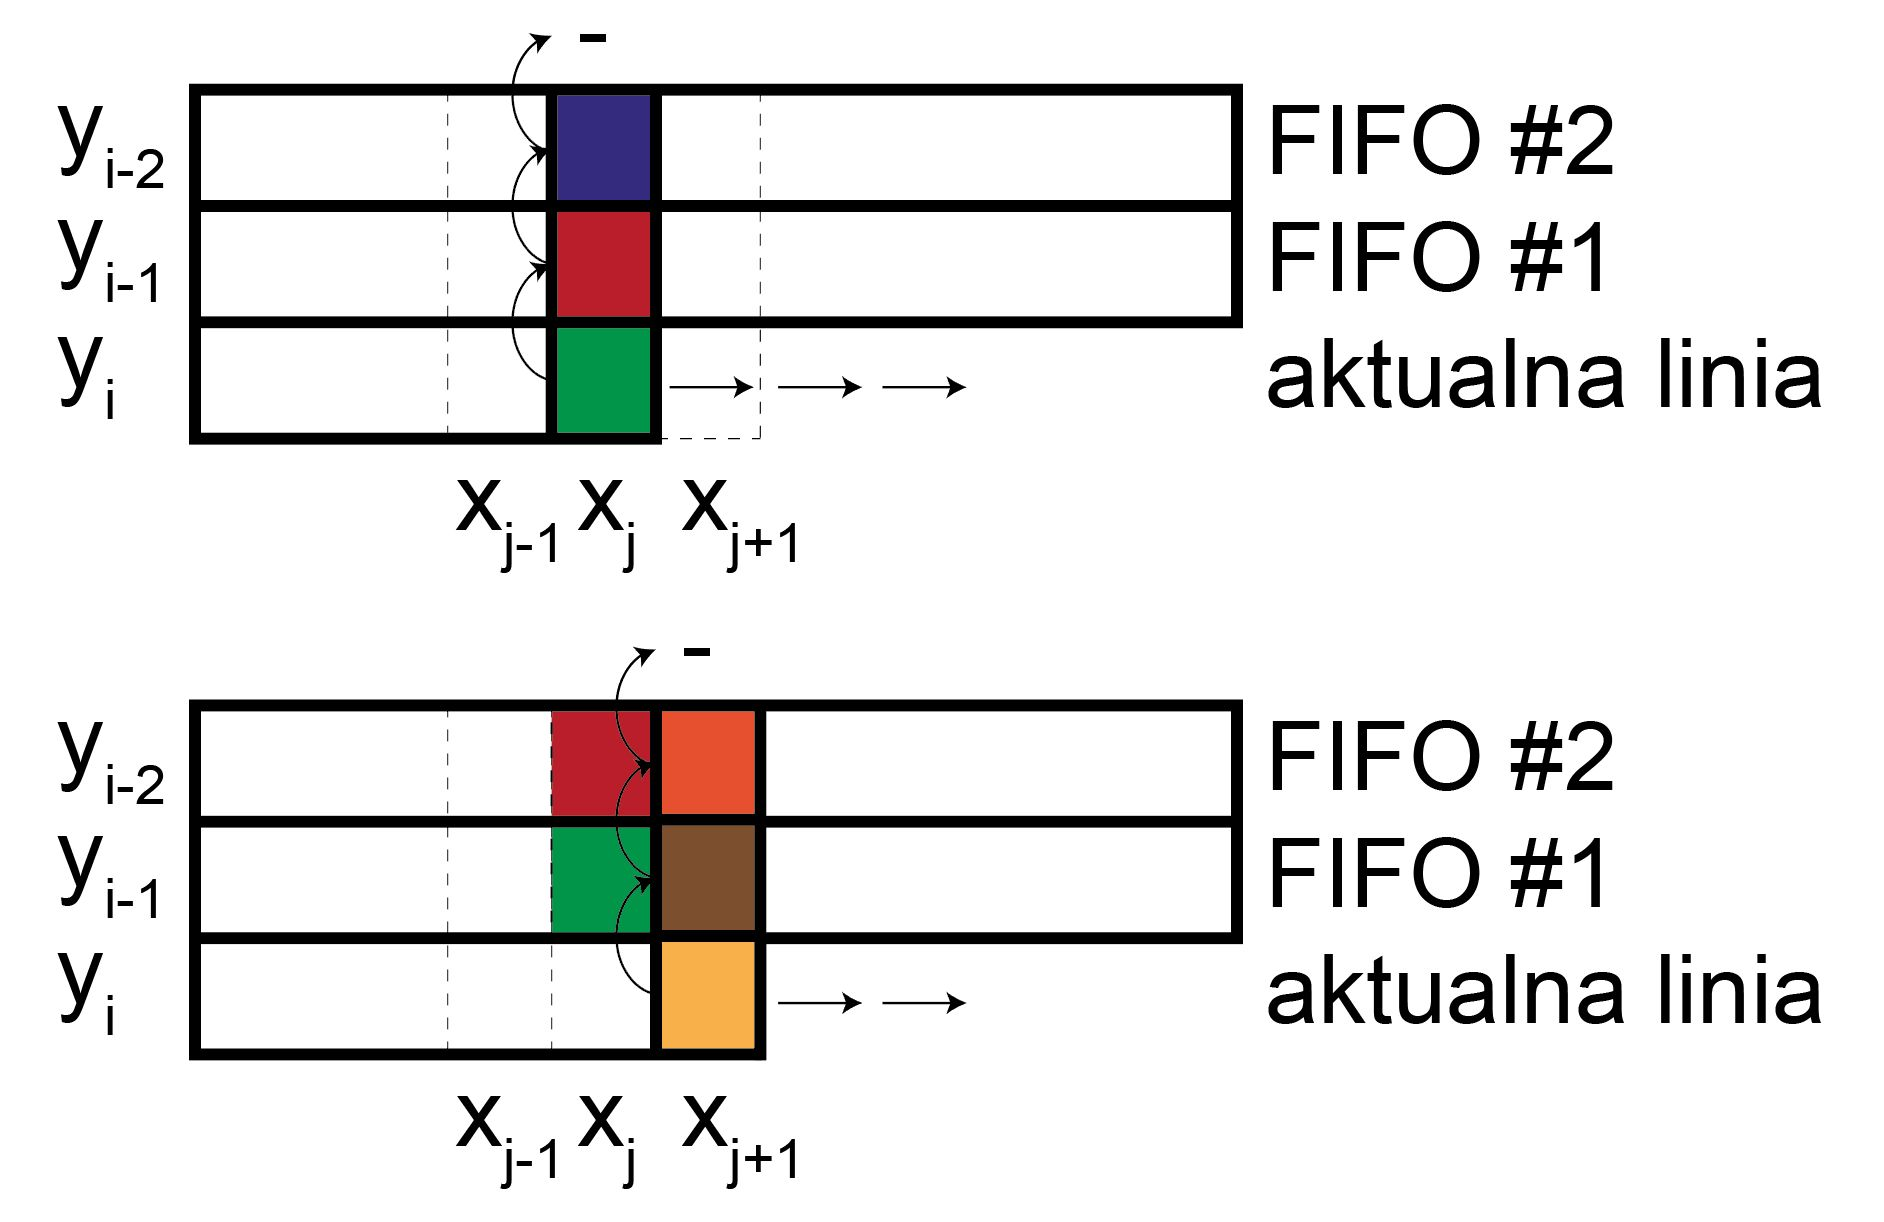
\includegraphics[width=11cm]{4_fifo_gradient.jpg}
	\caption{Schemat działania kolejek FIFO w procesie obliczania gradientu pionowego}
	\label{fig:fifo_gradient}
\end{figure}

Obliczanie gradientu poziomego nie nastręcza już tak wielu trudności -- sąsiadujące ze sobą piksele pojawiają się tuż po sobie, jednak w tym wypadku zamiast aktualnych wykorzystywane są piksele wychodzące z FIFO \#1 i zapamiętywane w rejestrze przesuwnym. 
Oznacza to, że w~chwili pojawienia się na wejściu do modułu nowego piksela ($i,j$), obliczony zostanie gradient poziomy piksela ($i-1,j-1$). 
Przez tę latencję potrzebne jest również nieznaczne opóźnienie gradientu pionowego, by obie wartości były zsynchronizowane i ustawione na wyjściu w tym samym momencie.

Sytuacje opisane powyżej dotyczą gradientów dla pikseli wewnątrz obrazu. 
Dla piksela znajdującego się na „początku” obrazu (lewa oraz górna krawędź), gradientem będzie dwukrotność różnicy pomiędzy nim a jedynym jego sąsiadem -- w odpowiedniej osi. %TODO nie na początku tylko na brzegu. Swoja drogą to normalnie się to pomija. %ODP pomija się opis, czy obliczenia gradientów brzegowych? 
%TODO 2 Obliczenia gradientu na brzegach %ODP OK, skoro mam już to wypada napisać, bo ta logika trochę mi zżarła nerwów;)

Poprzednie obliczenia były przeprowadzane w oparciu o sygnał aktywnego piksela ($valid$), którego zbocza były wykorzystywane do określenia gradientów aż do przedostatniego wiersza i~kolumny obrazu ($i-1, j-1$).
Piksele znajdujące się przy prawej i dolnej krawędzi ekranu wymagają innego podejścia. 
W tym przypadku, wymagane było stworzenie logiki kontynuującej obliczenia i generującej wyjściowe sygnały aktywne pomimo brak sygnału ($valid$). 
Opisywana sytuacja to również brak nowych wartości pikseli dla kolejek FIFO, co skutkuje ich spodziewanym opróżnieniem krótko po odebraniu pełnej ramki obrazu.
O ile poprzednio tempo obliczania kolejnych gradientów było podyktowane obecnością nowych pikseli, to w tym przypadku logika korzysta wyłącznie z opróżnianych kolejek FIFO, redukując odstęp pomiędzy wynikami do minimum (1 cykl zegara), co jest w zasadzie bez znaczenia dla dalszych obliczeń, które korzystają z poprawnie wygenerowanego sygnału aktywnego sygnalizującego obecność wyniku na wyjściu.


\subsection{Histogram gradientów}

%TODO 2 - Zacząć, że w pierwszym kroku moduł i kąt. I to nieco uporządkować, bo na mój gust jest pomieszany moduł i atan  w opisie. %ODP racja

Wyznaczone gradienty służą następnie do obliczenia modułu i kąta. 

Fragment logiki odpowiedzialny za obliczenie modułu został zrealizowany przy użyciu dwóch mnożarek dla obu gradientów, a sumę ich kwadratów następnie poddano pierwiastkowaniu w bloku CORDIC \cite{CORDIC}. 
Moduł będzie rozpoczynać obliczenia dla danych wejściowych tylko w przypadku, gdy policzone zostały oba gradienty (dwa niezależne sygnały \textit{valid\char`_x/y}) oraz gdy przynajmniej jeden z nich jest różny od zera ($\frac{0}{0}$ jest elementem nieoznaczonym, z~którego nie sposób policzyć implementowaną funkcję). 
Opisane warunki \textit{valid\char`_x/y}, połączone odpowiednimi operatorami logicznymi, wyprowadzono jako sygnał aktywny modułu. 

Z kolei wartość kąta jest obliczana w oparciu o wyrażenie $arctg(\frac{g_y}{g_x})$. Wykorzystano tutaj również blok IP CORDIC, który na wejściu otrzymuje wektor złożony z licznika oraz mianownika o tych samych długościach, przy czym jego całkowita długość jest zaokrąglana do wielokrotności liczby 16. Gradienty uzyskane z poprzedniego modułu są zapisane w notacji S9.1, zatem wektor wejściowy musi mieć długość 32 -- po 16 bitów na oba gradienty.
Bardziej znaczące bity tych połówek zostały wypełnione zerami i nie mają znaczenia dla obliczeń.

Otrzymane wartości należy następnie umieścić w dziewięciu 20-stopniowych przedziałach, co opisuje schemat \ref{fig:hog_gradient}. 
\begin{figure}[!ht]
	\centering
	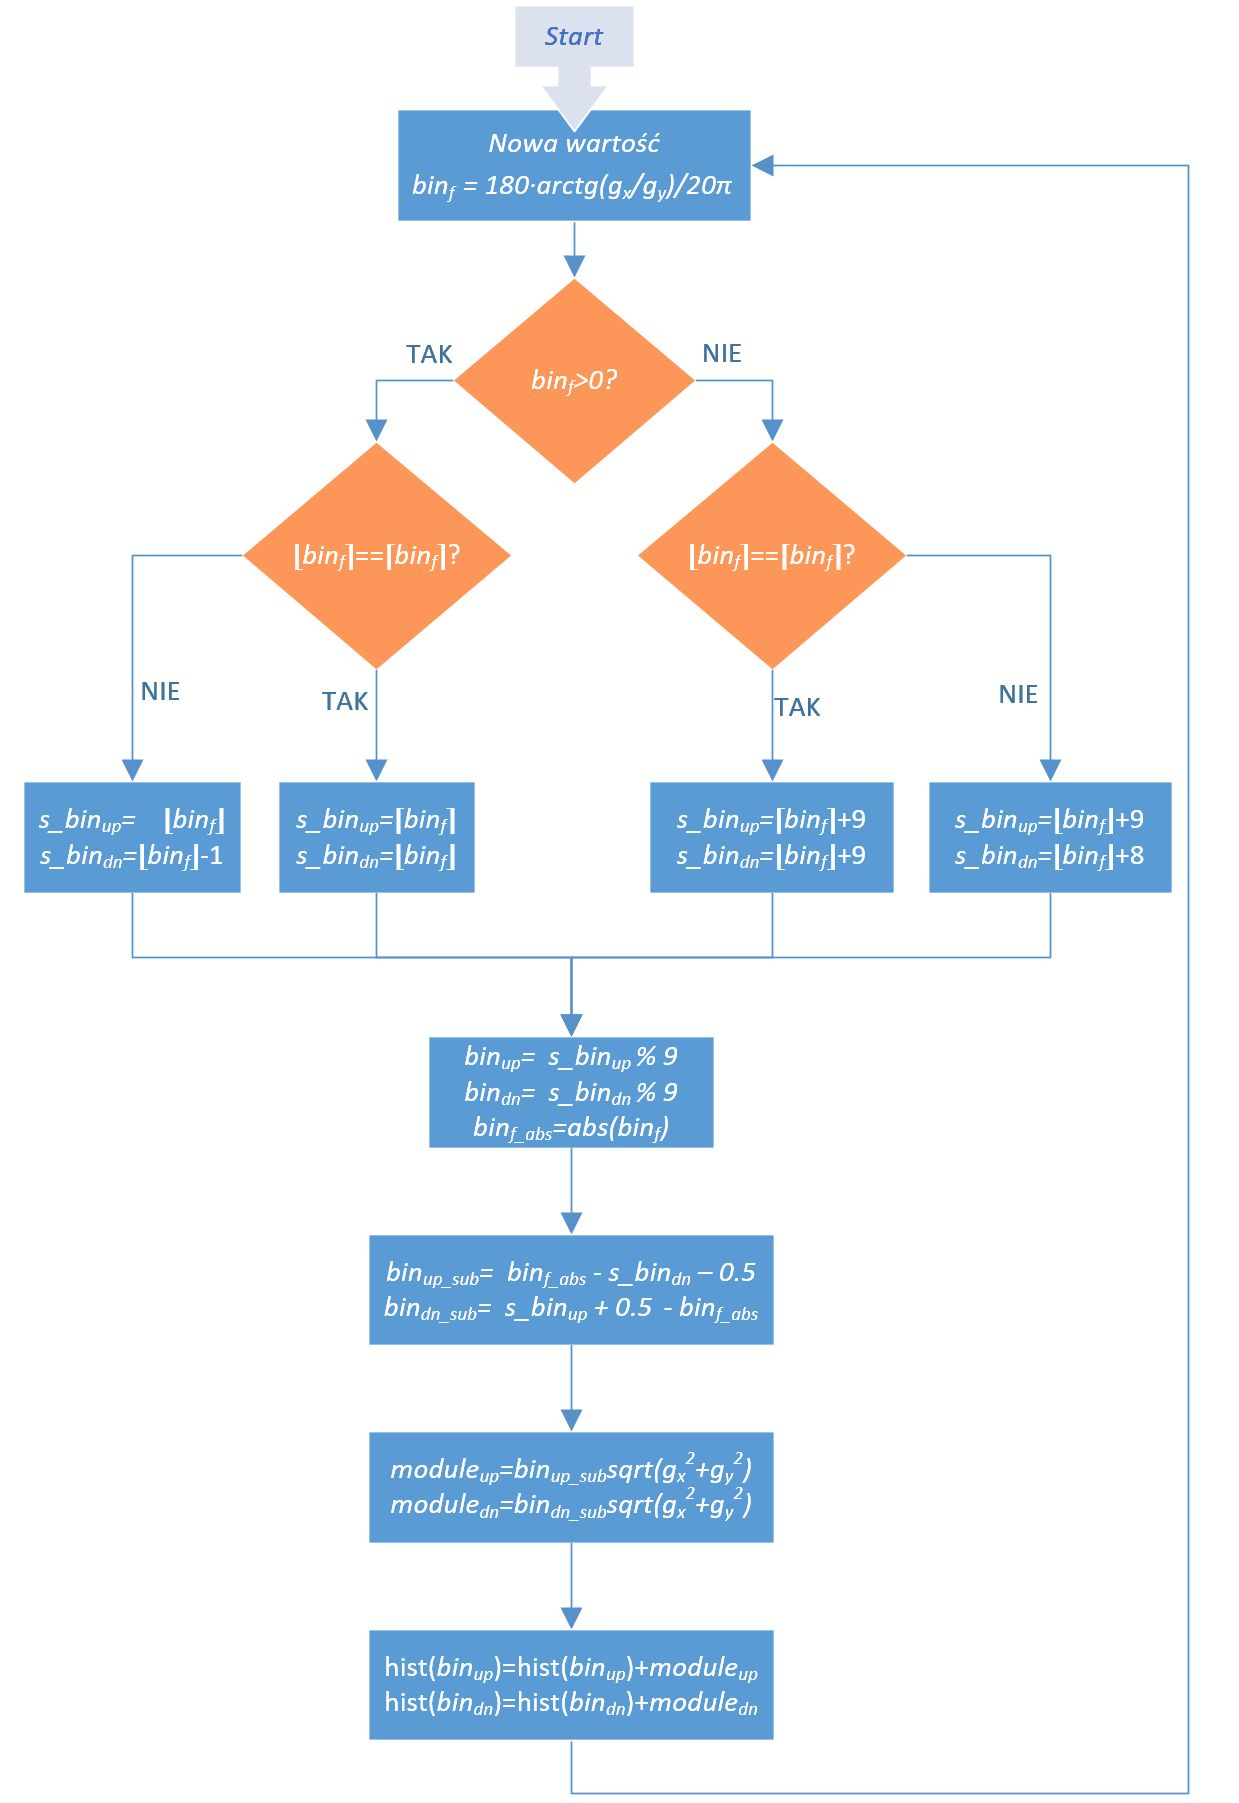
\includegraphics[width=12cm]{4_HOG_gradients.jpg}
	\caption{Schemat obliczeń histogramu gradientów}
	\label{fig:hog_gradient}
\end{figure}

Pierwszym krokiem jest operacja mnożenia kątów podanych w radianach przez $\frac{180}{20\pi}$, która konwertuje je do liczb ułamkowych stanowiących wstępny przydział (niech będzie to $bin_f$).

Następnie, w zależności od położenia względem środka danego przedziału, wybierane są przedziały: górny i dolny w postaci liczb całkowitych: $s\_bin_{up}$ oraz $s\_bin_{dn}$. 
Ostateczne będą one jednak wymagać normalizacji do postaci liczb z zakresu 0-8 i dopiero wówczas
dwa przedziały histogramu zostaną powiększone o interpolowane wartości modułu gradientów. 

W procesie obliczania modułu, suma mnożeń podnoszących gradienty do kwadratu jest wektorem U21.2, który poprzez dopisanie bitu '0' rozszerzono do U21.3. 
Zgodnie z dokumentacją bloku CORDIC, wektor o tej długości jest traktowany jako U1.23 -- zatem jest wirtualnie przemnożony przez $2^{20}$. 
Wartość wyjściową należy później interpretować jako U11.13 (wirtualnie podzieloną przez $\sqrt{2^{20}}=2^{10}$). 
Podstawową informacją wykorzystywaną w interpolacji jest odległość $abs(bin_f)$ od środków przedziałów $s\_bin_{up}$ oraz $s\_bin_{dn}$. 
Na tej podstawie obliczane są $module_{up}$ oraz $module_{dn}$, których suma jest równa pełnemu modułowi gradientów.
Ostateczne informacje -- to jest dane o przedziałach i odpowiadające im części modułu zostały przekazane dalej, wraz z wygenerowanymi sygnałami aktywnymi, które oznaczają obecność wyniku. 

Cały powyższy fragment podrozdziału skupiał się na operacjach związanych z pojedynczym pikselem. 
Teraz należy spojrzeć jednak z innej perspektywy, mianowicie na grupowanie pikseli w komórki, bloki i tworzenie wektorów cech na podstawie histogramu. 

Najlepszy możliwy rezultat detekcji osiąga się analizując i klasyfikując jak największą liczbę okien detekcji w danym obszarze zainteresowań. %TODO 2 niejasne, chodzi Panu o liczbę okien detekcji ?  %ODP poprawiono
Te powinny być wygenerowane dla fragmentów obrazu, których przesunięcie względem siebie jest jak najmniejsze -- zilustrowano to na rysunku \ref{fig:HOG_mesh}. 
Wektory cech są zapisywane w pamięci BRAM, jednak szybki przyrost zużycia zasobów układu ogranicza implementację do przetwarzania jedynie określonej liczby obszarów w sąsiedztwie miejsca estymowanej lokalizacji postaci -- dane te muszą być przechowane jednocześnie do momentu zakończenia klasyfikacji.

By nie zużywać cennego miejsca w blokach BRAM, zdecydowano się zapisywać histogramy a nie znormalizowane w~blokach wektory cech -- wiedząc, że dalsza logika dokonując odczytu z tej pamięci w odpowiedni sposób przekaże te informacje do klasyfikatora. 
Ostatecznie, pojedyncze okno detekcji $128\times 64$ to $32\cdot16=512$ histogramów, czyli $4608$ wartości. 
Wektor cech to aż $31\cdot15\cdot4\cdot9=16740$ wartości. 
Oszczędność wynikająca z zapisu pojedynczych histogramów pozwoli utworzyć znacznie więcej wektorów cech. 
Przykładowo, dla okna o wielkości $144\times 96$ należy zapisać $7776$ wartości. 
Pozwala to jednak wygenerować $9\cdot5=45$ wektorów cech. 
Gdyby zaś wpisywać je do pamięci w gotowej formie, wymagałoby to aż $16740\cdot45=753300$ elementów. 

Pamięć RAM należy potraktować jako zbiór 9-elementowych histogramów ułożonych obok siebie. 
Przetwarzanie obrazu, rozumianego jako obiekt dwuwymiarowy, wymaga odpowiedniego mapowania tworzonych wartości do postaci jednowymiarowej, adresowej. 
Schemat \ref{fig:hog_histogram_scheme} przedstawia działanie logiki na ramce obrazu w kontekście zapisu histogramów do pamięci. 
Symbolem „$<=$” określa się przypisanie nieblokujące, które rzeczywisty efekt będzie miało dopiero na następnym zboczu narastającym zegara (i może być zastąpione kolejnym przypisaniem w obrębie jednego cyklu zegara).
 
\begin{figure}[]
	\centering
	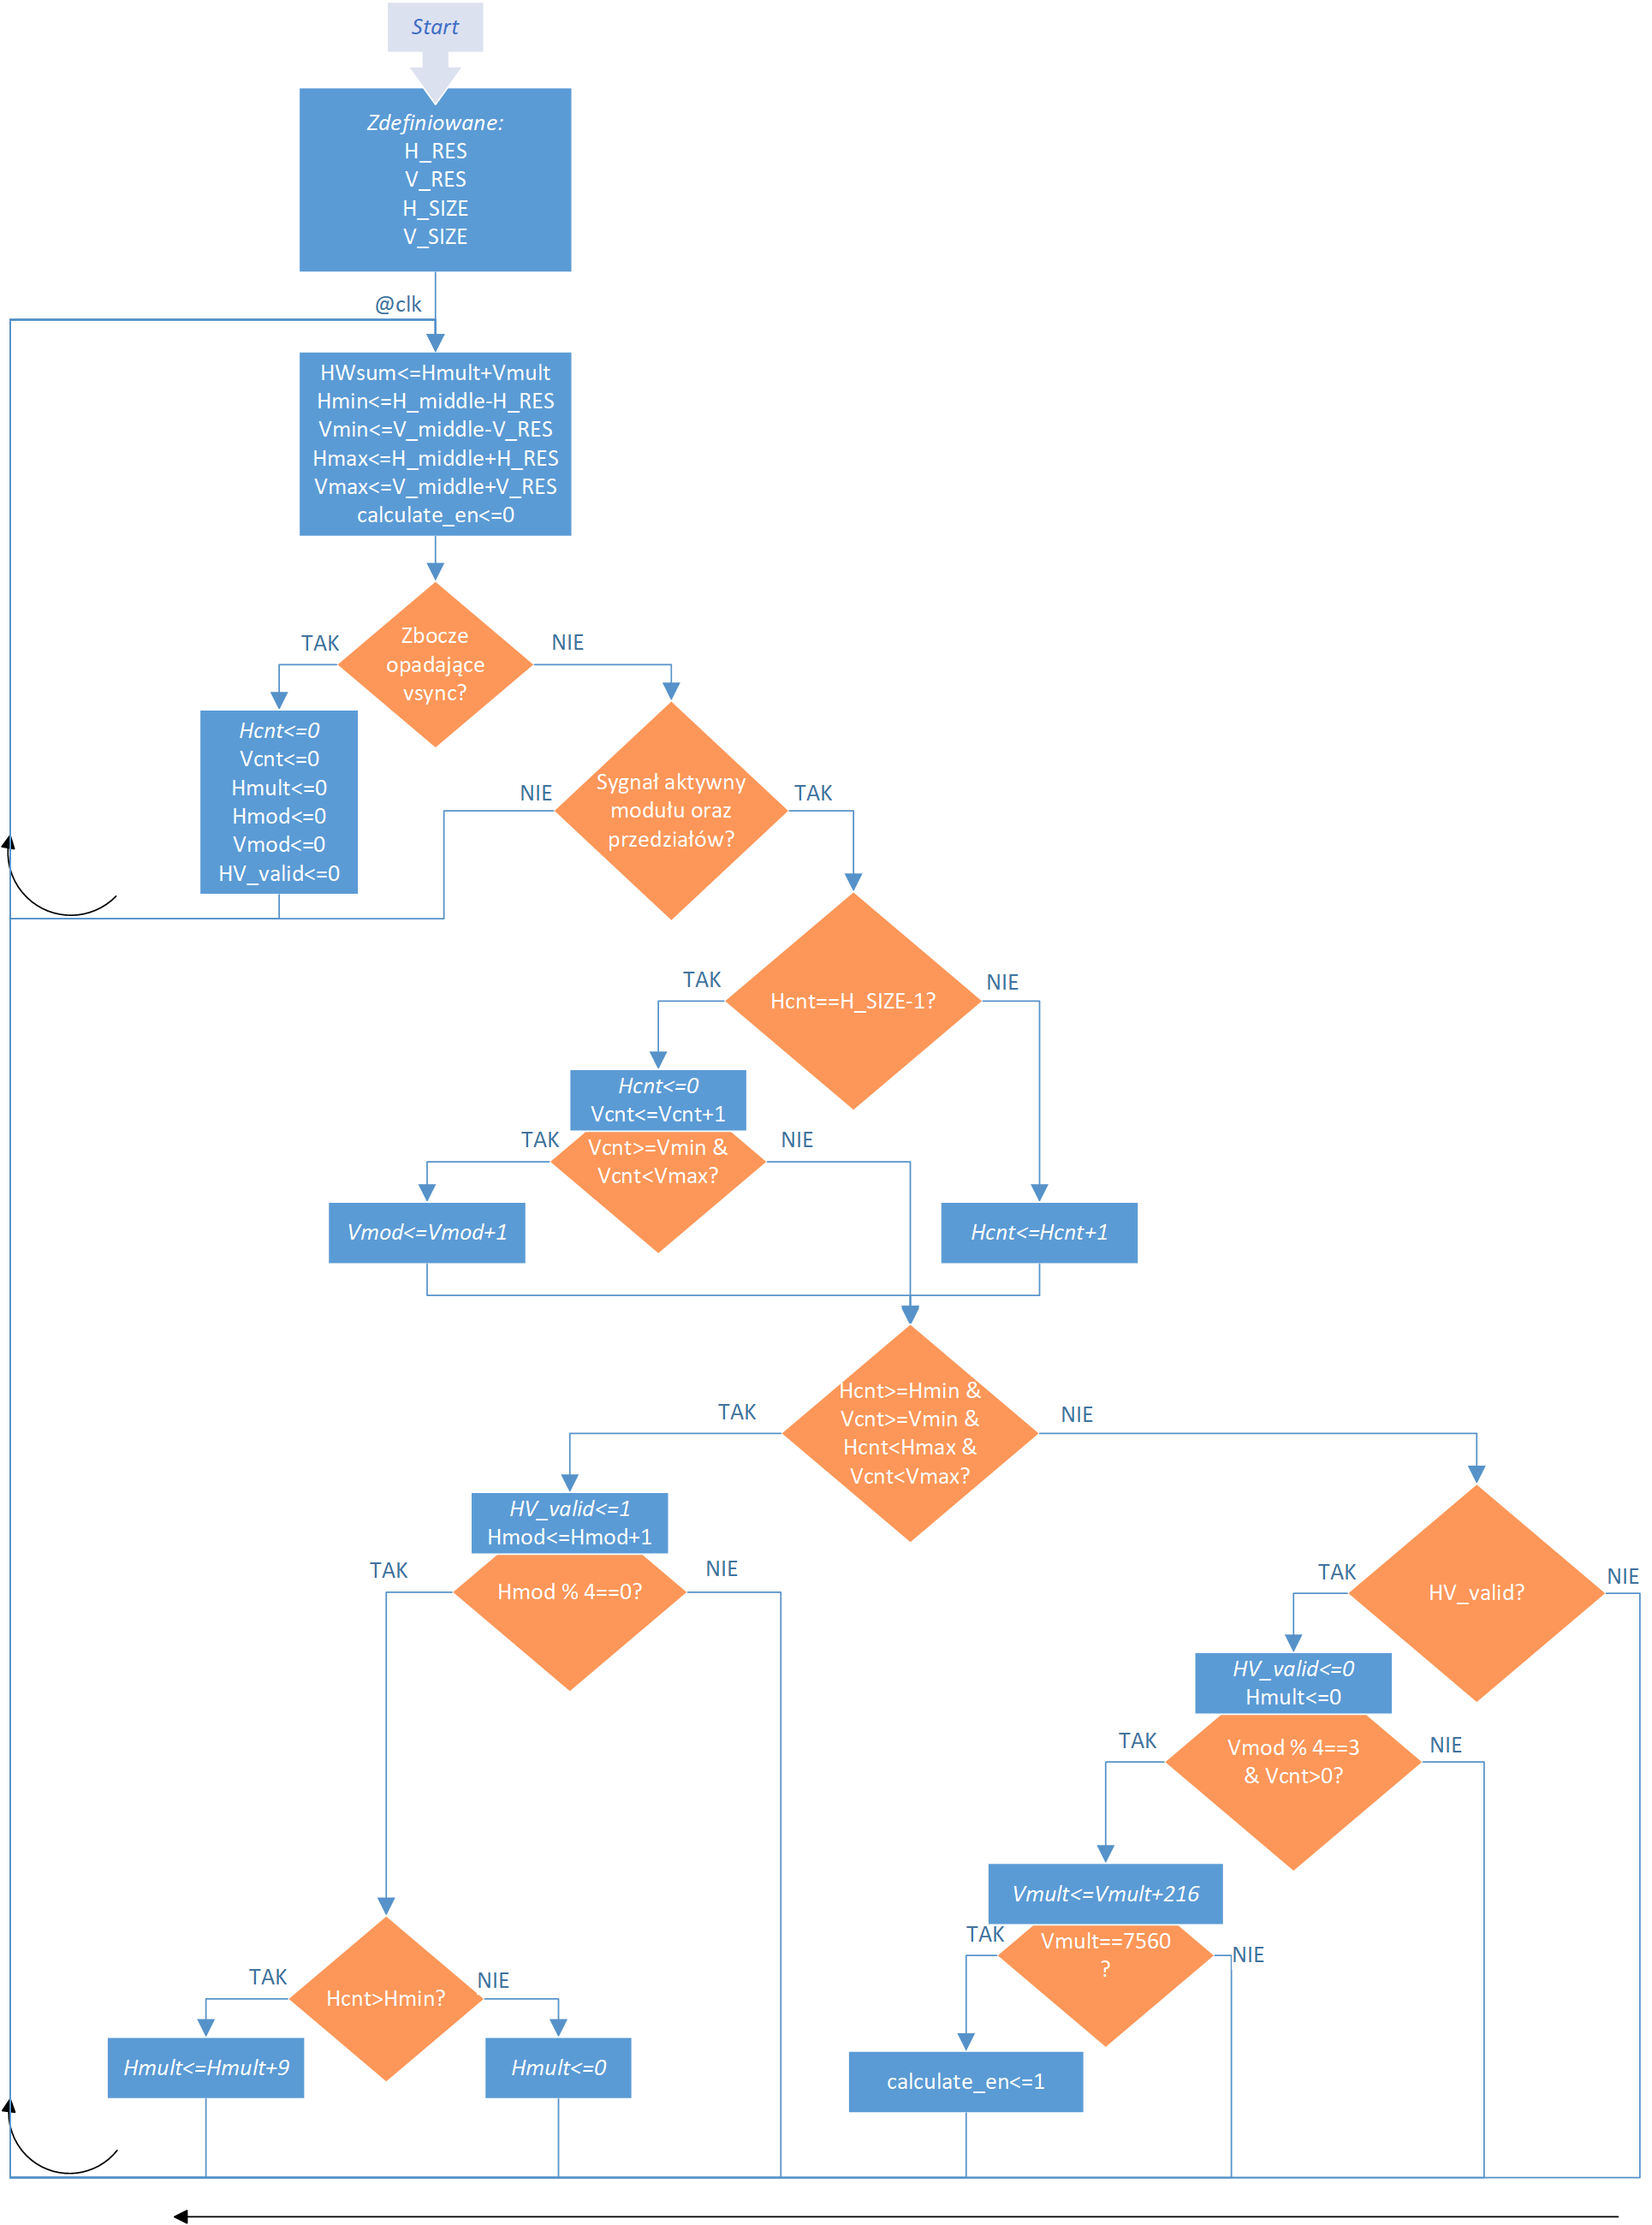
\includegraphics[width=16cm]{4_HOG_Histograms.png}
	\caption{Procedura wyboru adresu pamięci RAM w oparciu o pozycję aktualnego piksela}
	\label{fig:hog_histogram_scheme}
\end{figure} 
 
Określenie aktualnego położenia na obrazie jest możliwe dzięki zastosowaniu liczników, opierających swoje działanie na obecności sygnału aktywnego sygnalizującego gotowe dane wejściowe.
Wykorzystano następujące parametry:
\begin{itemize}
	\item \textit{H\_SIZE}, \textit{V\_SIZE} -- rozdzielczość obrazu przeskalowanego (indywidualnie dla każdej skali),
	\item \textit{H\_middle}, \textit{V\_middle} -- współrzędne piksela środkowego, będącego w centrum analizowanego obszaru (w odniesieniu do odpowiedniej skali, dostarczone przed rozpoczęciem analizy pełnej klatki),
	\item \textit{H\_RES}, \textit{V\_RES} -- wartości określające zasięg analizowanego obszaru -- w odległości od piksela środkowego - dla tego projektu są to odpowiednio: $96/2=48$ oraz $144/2=72$,
\end{itemize}
oraz zmienne:
\begin{itemize}
	\item \textit{Hcnt}, \textit{Vcnt} -- zmienne inkrementowane odpowiednio do wartości maksymalnych \textit{H\_SIZE}, \textit{V\_SIZE} -- pozwalają określić aktualne położenie na obrazie (i względem analizowanego obszaru),
	\item \textit{HV\_valid} -- sygnał aktywny, który wysokim stanem informuje o aktualnym położeniu wewnątrz analizowanego obszaru,
	\item \textit{Hmod}, \textit{Vmod} -- liczniki modulo służące do rozdzielenia pikseli wchodzących w skład różnych histogramów (kwadratów o boku $4\times 4$),
	\item \textit{Hmult}, \textit{Vmult} -- zmienne będące bazą adresową do zapisu aktualnego histogramu (horyzontalna zmienna powiększana o $9$, wertykalna o $9\cdot24$ -- liczba histogramów w linii poziomej),
	\item \textit{calculate\_en} -- sygnalizacja zakończonego procesu obliczania i zapisywania histogramów -- gotowość do rozpoczęcia normalizacji i klasyfikacji dla danej skali. 
\end{itemize}

Logika, działająca niezależnie dla każdej skali, jest reinicjalizowana po odebraniu sygnału nowej ramki (\textit{vsync}). 
W momencie otrzymania informacji o kolejnym zestawie przedziałów i~modułu, liczniki \textit{Hcnt} oraz \textit{Vcnt} określają jego obecność względem oczekiwanego obszaru detekcji. %TODO 2 to warunkują źle brzmi... %ODP OK
Jeśli analizowany zestaw danych przynależy do obszaru, liczniki modulo \textit{Hmod} i \textit{Vmod} są inkrementowane -- odpowiednio co każdy piksel w obszarze, oraz co kolejną linię w obszarze. 
Podzielność któregokolwiek z nich przez 4 oznacza zmianę histogramu dla kolejnych danych -- wymaga to powiększenia rejestru \textit{Hmult} o 9, lub \textit{Vmult} o 216. 
Ostatecznie, dostępy do odpowiednich adresów pamięci są przedstawione równaniem:
\begin{equation}
\label{eq:adressing_hist}
\left.\begin{aligned} 
addr_{up}&=Hmult+Vmult+s\_bin_{up} \\ 
addr_{dn}&=Hmult+Vmult+s\_bin_{dn}
\end{aligned}\right.
\end{equation}
Pamięć histogramu pracuje w trybie True Dual Port, umożliwiając jednoczesny dostęp do dwóch interpolowanych przedziałów aktualnego histogramu, $s\_bin_{up}$ oraz $s\_bin_{dn}$. 
Zapis danych do pamięci histogramu jest realizowany po odczycie aktualnych wartości komórek i powiększeniu ich o odpowiednie części modułu: $module_{up}$ oraz $module_{dn}$.


\subsection{Uczenie}
Założeniem jest, by podczas pracy systemu wbudowanego nie ingerować we współczynniki, a opierać się na pierwotnych wynikach uczenia.
Dane te muszą być przechowane w odpowiedni sposób, by możliwy był do nich prosty i szybki dostęp. 
Postanowiono zapisać wektor w pamięci ROM inicjalizowanej plikami typu \textit{*.mem}, utworzonymi podczas wykonywania skryptu uczenia w MATLABie.
Ręcznie dostosowany moduł pamięci posiada trzy niezależne sektory (w~zakresie adresowania i~długości danych), inicjalizowane następującymi informacjami: 

\begin{itemize}
	\item składniki skalujące \textit{shifts} -- 16740 elementów wymaganych do przesunięcia każdego elementu wektora cech. Wartości w przedziale: \mbox{$<-0.2616, -0.0527>$}; precyzja zapisu: S0.11.
	\item współczynniki maszyny wektorów nośnych \textit{vectors}. Wartości w przedziale: \mbox{$<-0.0076, 0.0063>$}; precyzja zapisu: S0.27 (w formacie S0.23, lecz 4 najstarsze bity mają zawsze postać bitu znaku).
\end{itemize}


Dodatkowym współczynnikiem jest wartość przesunięcia gotowego wyniku o precyzji S0.40, jednak jest ona przechowywana w logice. 
Powyższa pamięć zajmuje aż 36 z wszystkich 140 bloków BRAM dostępnych w rozważanym układzie. 
Należy zauważyć, iż wymusza to współdzielenie pojedynczej instancji modułu we wszystkich procesach klasyfikacji. 
Z tego względu istotne jest stworzenie logiki synchronizującej początek przetwarzania wektorów cech ze wszystkich skal -- opisane jest to w~kolejnym podrozdziale.

\subsection{Klasyfikacja}


Po obliczeniu wektorów cech następuje proces klasyfikacji. 
Poprzedza ją normalizacja w~blokach, która jest częścią tego modułu -- ze względu na obecność każdego histogramu w~kilku różnych blokach. 
Odczytywane z pamięci ROM wartości współczynników klasyfikatora muszą być współdzielone pomiędzy obliczeniami przeprowadzanymi dla każdej ze skal obrazu, jednak w każdym przypadku tempo generowania histogramów nie jest jednakowe -- proces ten przebiegnie szybciej dla większych obrazów (tam analizowany fragment obrazu pojawi się na wejściu wcześniej). 
O gotowości histogramów z odpowiedniej skali informuje indywidualny dla niej sygnał \textit{calculate\_en}. 
Dopiero w momencie otrzymania wszystkich sygnałów \textit{calculate\_en} (stan wysoki na wyjściu iloczynu logicznego) rozpoczynany jest właściwy proces klasyfikacji.

Moduł odpowiadający za sklasyfikowanie informacji pochodzących z pojedynczej skali zrealizowano w formie krótkiej maszyny stanu, na którą składają się następujące etapy:
\begin{itemize}
	\item inicjalizacja -- oczekiwanie na sygnał \textit{full\_frame}, informujący o rozpoczęciu algorytmu na pełnej klatce obrazu
	\item czyszczenie pamięci przechowującej wektory cech z poprzednich uruchomień algorytmu -- etap ten ma miejsce tuż po otrzymaniu sygnału \textit{full\_frame}, który pojawia się podczas stanu wysokiego synchronizacji pionowej; jest wykonywany na tyle szybko, by pamięć mogła być  zapisana wartościami histogramów z nowej ramki obrazu 
	\item oczekiwanie na iloczyn sygnałów \textit{calculate\_en}; inicjalizacja zmiennych algorytmu
	\item właściwa normalizacja i klasyfikacja
\end{itemize}

O ile zapisane w pamięci ROM współczynniki mają postać wektora cech, tak pamięć RAM przechowuje nieuporządkowane fragmenty histogramów. 
Wymagało to stworzenia logiki, która łączy ze sobą dane ze ściśle określonych adresów pamięci, interpretując je w postać deskryptora.  
Opisuje to diagram \ref{fig:hog_feature_histrogram_address}.

\begin{figure}[h!]
	\centering
	\captionsetup{justification=centering,margin=1cm}
	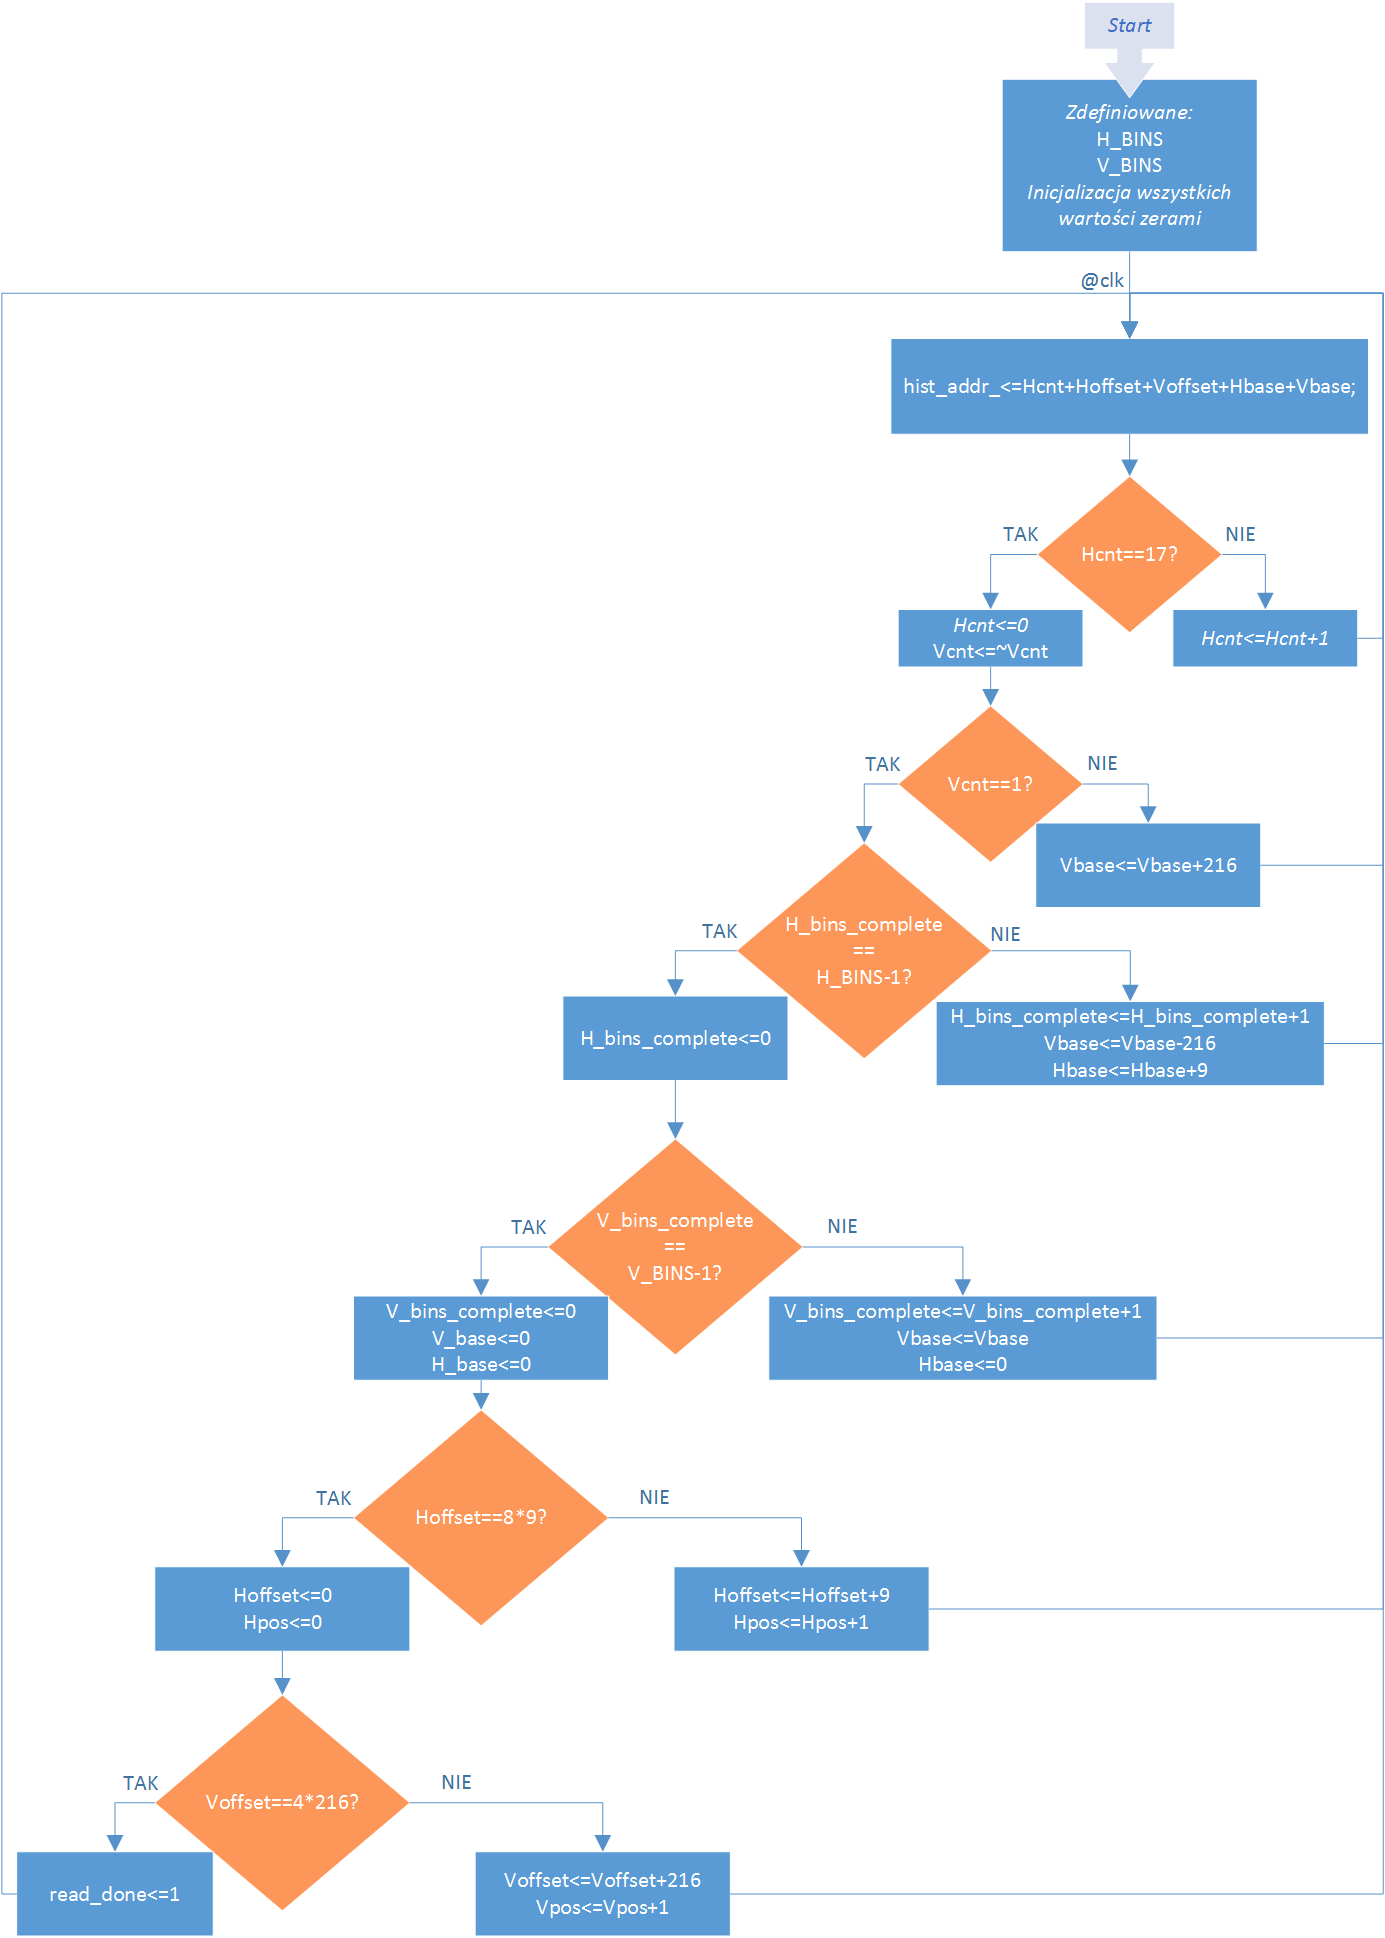
\includegraphics[width=15cm]{4_HOG_Features.png}
	\caption{Procedura wyboru adresu pamięci RAM w procesie odczytu kolejnych histogramów}
	\label{fig:hog_feature_histrogram_address}
\end{figure} 

Kolejnym etapem jest normalizacja w blokach, która ze względu na prostszą realizację została umieszczona wewnątrz procesu klasyfikacji (tym bardziej, że idea bloków właściwie nie funkcjonowała we wcześniejszych modułach). 
Blokiem jest struktura 4 histogramów, czyli łącznie 36 wartości. 
Odczytane z pamięci RAM dane są podnoszone do kwadratu przez mnożarkę, a~następnie sumowane z kolejnymi wynikami. 
Suma 36 takich wartości, dodatkowo zinkrementowana, jest poddawana pierwiastkowaniu i będzie stanowić mianownik w procesie normalizacji powiązanego bloku (zgodnie z równaniem \eqref{eq:HOG_norm3}). 
Moduł pierwiastkujący działa potokowo, więc zwraca również wartość pierwiastkową z niepełnych sum -- dlatego ważne jest wygenerowanie sygnału aktywnego w momencie zsumowania 36 elementów, a także zatrzaśnięcie poprawnej wartości pierwiastka na czas 36 dzieleń.

Normalizacja wymusza ponowne odczytanie danych z pamięci RAM. 
Zastosowanie dwuportowego modułu pozwala na uzyskanie dostępu do uprzednio przetworzonych danych na drugim porcie, podczas gdy pierwszy kontynuuje zwracanie informacji potrzebnych do obliczenia współczynników normalizacji dla kolejnych bloków. 
Poprawną kolejność danych na drugim porcie osiągnięto przez odpowiednie opóźnienie sygnału adresowego z portu pierwszego. 

Napływające potokowo dane z portu drugiego, podzielone przez odpowiedni współczynnik normalizacji, mają ustawioną flagę \textit{normalized\_valid}.
Jej stan wysoki rozpoczyna inkrementację adresu pamięci ROM przechowującej współczynniki przesunięć (\textit{shifts}) pochodzące z procesu uczenia. 
Każda z 16740 par zostanie do siebie dodana. 
Znormalizowane elementy wektora cech mają postać U11.13, zatem należało uprzednio rozszerzyć wektor \textit{shifts} do tego formatu. 

Kolejnym krokiem jest wymnożenie każdej z sum przez właściwy współczynnik maszyny wektorów nośnych. 
Aby to osiągnąć, należało ponownie i odpowiednio opóźnić linie adresowe uzyskujące dostęp do przestrzeni adresowej danych oraz \textit{vectors}. 
Ostateczna szerokość pojedynczego elementu wynosi S7.40.

%TODO 2 teraz już oczywiście za późno, ale... normalnie SVM to by było 16740 wag i jeden bias. Nie wiem dlaczego w Matalabie jest ten shift, choć to da się wyeliminować - gdzieś jest pokazane jak. No można też przegłówkować :) Tak na przyszłoć, no bo to by zmiejszyło to zapotrzebowanie na pamięć. Może Pan takie jedno zdanie dorzucić do future work. %ODP racja... dopisano na końcu

Docelowa wartość definiująca detekcję jest sumą wszystkich 16740 przetworzonych elementów oraz jeszcze jednej stałej wyznaczonej na etapie uczenia, \textit{offset} równej $-0.6327$. 
\mbox{\textit{Offset}} stanowi wartość początkową sumy przy rozpoczęciu obliczeń dla kolejnego wektora cech.
Ze względu na konieczność zapewnienia dobrej dokładności w procesie sumowania, wynik jest zapisywany w notacji S7.40.

\subsection{Przetwarzanie wyników}

Niezależnie od liczby przetwarzanych skal obrazu, etap klasyfikacji jest dla nich realizowany równolegle, przetwarzając po $5\times 9$ wektorów cech i zakończy się w tym samym momencie. 
Zarówno tworzenie deskryptorów, jak i klasyfikacja są zaimplementowane w modułach działających w oparciu o zegar $148.5$MHz. 
Pozwala to zrealizować sam etap klasyfikacji w~czasie ok. $5$ms.

Kolejnym etapem jest analiza wyników ze wszystkich skal.
Jest on dość prosty, gdyż zakłada jedynie porównanie najlepszych rezultatów -- w modułach klasyfikacji każdej ze skal zaimplementowano logikę, która zapamiętuje swoje lokalne minima i parametry obszarów (w~odpowiednich skalach), na podstawie których je osiągnięto. 
Skutkiem porównań jest wyłonienie skali z najlepszym wynikiem, a koordynaty tego obszaru zostają dostosowane do rozdzielczości $1280 \times 720$ i mogą być wykorzystane przez warstwę wyższą. 

\section{Integracja układu FPGA z dronem}

Opisana w poprzednim podrozdziałach architektura sprzętowa dotyczyła dwóch algorytmów, które mogą funkcjonować niezależnie od siebie. 
Istnieje jednak jeszcze najwyższa warstwa logiczna, która łączy ich działanie, zwiększając niezawodność działania systemu. 
Na podstawie ostatecznych wyników śledzenia podejmowane są decyzje związane z ruchem drona. 
Muszą być one przekazane niezależnej jednostce odpowiedzialnej za stabilizację drona -- autopilotowi. 
Wymagało to m.in. określenia sposobu komunikacji pomiędzy nim a układem Zynq.



\subsection{Zdalne uruchomienie pracy systemu}

Początkowo stworzono (i ostatecznie pozostawiono) możliwość rozpoczęcia pracy algorytmów z wykorzystaniem jednego z przełączników na płycie PYNQ, gdyż prace nad projektem wymagały dość częstego uruchamiania algorytmu jeszcze bez udziału drona. 
Jednak lot maszyny lub nawet jego start praktycznie wyklucza fizyczny dostęp do układu FPGA, dlatego koniecznością stało się zdalne wyzwolenie pracy algorytmów. 
Sygnał wyzwalający nosi nazwę \textit{trigger\char`_algorithm}.

Podczas lotu maszyny użytkownik ma pod ręką jedynie aparaturę radiową, z poziomu której może jednak w dość prosty sposób wysyłać sygnały. 
Aparatura jest bowiem wyposażona w szereg konfigurowalnych przełączników analogowych i cyfrowych. 
Ponadto, dane są wysyłane poprzez 16 kanałów -- przy czym do kontroli podstawowych funkcji drona wykorzystuje się zaledwie 4. 
Wybrano zatem jeden z pozostałych dostępnych kanałów, któremu przypisano funkcję trzypoziomowego przełącznika obecnego na panelu urządzenia radiowego.

Sparowany z aparaturą odbiornik, który jest zamocowany na dronie, wysyła wszystkie dane po jednym zestawie przewodów w formie PPM (ang. \textit{Pulse Position Modulation}). 
Taki sygnał musiałby być zdekodowany w części PL układu Zynq w~celu uzyskania użytecznej wartości
Proces dekodowania rozwiązuje jednak autopilot, który konwertuje 16-kanałowy PPM na znacznie prostsze sygnały PWM (ang. \textit{Pulse Width Modulation}) m.in. do kontroli silników.
Co więcej, urządzenie Pixhawk umożliwia przypisanie reszty kanałów transmisyjnych do pomocniczych wyjść PWM. 
Rozwiązanie to znalazło zastosowanie chociażby w ustawieniu wartości zadanych serwomechanizmom odpowiedzialnym za pracę gimbala kamery.

Za pomocą oprogramowania Mission Planner, służącego do konfiguracji autopilota, ustawiono zakres szerokości wysyłanego pulsu PWM na $1100-1900$ us.
Wybranie odpowiedniej wartości wyzwalającej pracę systemu wymagało dodatkowej weryfikacji, podczas której sprawdzono przypadek z wyłączoną aparaturą radiową (brak wejściowego sygnału PPM) i ewentualne błędy w transmisji PWM.
Do pomiarów zastosowano analizator logiczny ILA wbudowany w~środowisko Vivado i stworzono prosty licznik, który jest poddawany następującym operacjom:

\begin{itemize}
	\item kasowanie na zboczu narastającym sygnału wejściowego,
	\item inkrementację podczas aktywnego stanu sygnału,
	\item przypisanie tej samej wartości w każdym innym przypadku.
\end{itemize}

Logika jest taktowana zegarem \textit{calc\char`_clk} $=100$MHz i dla poszczególnych pozycji przełącznika na aparaturze radiowej wartości licznika są przedstawione w tabeli \ref{tab:RFswitch}. 
Pokazuje ona, że zakres długości pulsu nie odstaje od normy typowego sygnału PWM, mimo że jest nieco zawężony.

\newcolumntype{P}[1]{>{\centering\arraybackslash}p{#1}}
\begin{table}[h]
	\centering
	\caption{Szerokości pulsu PWM dla przełącznika odpowiedzialnego za start algorytmu}	
	\begin{tabular}{|P{3cm} |P{2cm} |P{2cm}|}
		
		\hline
		\rowcolor{lightgray} Pozycja przełącznika & Wartość licznika & Długość pulsu [ms]  \\ 
		-1	& 109000 & 1.09	\\ 
		\hline
		0	& 149000 & 1.49 \\ 
		\hline
		1	& 189000 & 1.89 \\ 
		\hline
	\end{tabular}
	\label{tab:RFswitch}
\end{table}

Na tej podstawie określono, że warunkiem koniecznym do rozpoczęcia algorytmu będzie wystąpienie dwóch kolejnych pulsów o szerokości przynajmniej 1.8 ms (górny limit przezornie ustawiono na 2 ms). 
Analogicznie, zakończenie pracy algorytmu i powrót do ustawień domyślnych będzie miał miejsce po zmianie pozycji przełącznika z „1”, czyli po otrzymaniu dwóch kolejnych pulsów o szerokościach spoza zakresu $[1.8$ ms,$2$ ms$]$.


\subsection{Kontrola pracy algorytmów MeanShift oraz HOG+SVM}

Najwyższa warstwa w części programowalnej Zynq jest odpowiedzialna za integrację działania algorytmów MeanShift i HOG+SVM i zarządza sygnałami używanymi do ich niezależnego uruchamiania. 

\subsubsection{Komunikacja pomiędzy PL i PS}

Nie jest to jednak najwyższy poziom zarządzania w~układzie PYNQ -- warstwa ta komunikuje się bowiem z aplikacją uruchomioną w części PS, która jest odpowiedzialna za nadzór nad pracą zarówno autopilota, jak i opisywanej do tej pory części PL układu Zynq.
Komunikacja pomiędzy PS a PL jest realizowana dwutorowo:
\begin{itemize}
	\item PL odbiera ustawienia konfiguracyjne z przestrzeni adresowej 32-bitowych rejestrów. Używanych jest 5 rejestrów, które są inicjalizowane w PS wartościami domyślnymi. Ich opis przedstawia tabela \ref{tab:registersIN}	
	\item PL wysyła informacje 32-bitowym sygnałem GPIO, który jest skonfigurowany w części PS do wywoływania przerwań po każdej jego zmianie. Utworzone są również 2 dodatkowe rejestry, z których dane odczytywane są w PS podczas obsługi tego przerwania. Strukturę przedstawia tabela \ref {tab:registersOUT}
\end{itemize} 

\newcolumntype{P}[1]{>{\centering\arraybackslash}p{#1}}
\begin{table}[h]
	\centering
	\caption{Informacje wysyłane do PS w postaci rejestrów}	
	\begin{tabular}{|P{1.4cm} |p{9.5cm}| p{1.25cm}| p{1.75cm}|}
		
		\hline
		\rowcolor{lightgray} Adres rejestru & Sygnały & Format & Pozycja w rejestrze  \\ 
	    -- (GPIO)	& \textbf{\textit{PL\_to\_PS\_control}} -- wymuszenie ruchu drona w oparciu o dane rejestru 0x04\newline
	    \textbf{\textit{PL\_to\_PS\_status}} -- status pracy algorytmów MS/HOG+SVM\newline
		\textbf{\textit{trigger\char`_algorithm}} -- rozpoczęcie misji (sygnał z~aparatury radiowej) & 
		U1.0  \newline\newline
		U4.0 \newline\newline
		U1.0  & [12:12]\newline\newline[7:4]\newline\newline[0:0]\\ 
		\hline
		0x04	& \boldmath{$y_{pos}$} -- odległość do punktu zadanego na osi x obrazu\newline
		\boldmath{$x_{pos}$} -- odległość do punktu zadanego na osi y obrazu\newline
		\boldmath{$z_{scale}$} -- wartość skali dla ostatnich detekcji & 
		S10.0  \newline
		S10.0 \newline
		U3.2  & [30:20]\newline[18:8]\newline[4:0] \\ 
		\hline

	\end{tabular}
	\label{tab:registersOUT}
\end{table}

\newcolumntype{P}[1]{>{\centering\arraybackslash}p{#1}}
\begin{table}[h]
	\centering
	\caption{Informacje odbierane z PS w postaci rejestrów}	
	\begin{tabular}{|P{2cm} |p{8cm}| P{1.5cm}| P{2cm}|}
		
		\hline
		\rowcolor{lightgray} Adres rejestru & Sygnał & Format & Wartość domyślna   \\ 
		0x00	& \textbf{\textit{PS\_to\_PL\_run\_alg}} -- kontrola pracy maszyny stanów w PL nadzorującej algorytmy MS/HOG+SVM: \newline0 - nieaktywna\newline1 - aktywna & U1.0& $0$\\ 
		\hline
		0x04	& \textbf{\textit{SVM\_threshold}} -- wartość progu & S7.24 &$-0.1$\\ 
		\hline
		0x08	& \textbf{\textit{SVM\_strong\_threshold}} -- wartość progu drugiego stopnia & S7.24 &$-1$\\ 
		\hline
		0x0C	& \textbf{\textit{SVM\_lost\_iter}} -- maksymalna liczba iteracji opartych wyłącznie na wyniku MeanShift & U15.0 & $100$\\ 
		\hline
		0x10	& \textbf{\textit{SVM\_iter\_between\_control}} -- liczba iteracji algorytmu SVM pomiędzy aktualizacjami uchybu regulacji do PS & U6.0 & $15$\\ 
		\hline
	\end{tabular}
	\label{tab:registersIN}
\end{table}
%TODO 2 a ten próg 2 stopnia to gdzieś był wcześniej wspomniany ? %ODP jest wspominany niżej

Do rozpoczęcia pracy algorytmów wymagane jest otrzymanie informacji o gotowości drona, czyli ustabilizowaniu jego pozycji w powietrzu. 
Służy do tego rejestr \textit{PS\_to\_PL\_run\_alg} opisany w tabeli \ref{tab:registersIN}.



\subsubsection{Pierwsza detekcja osoby}

Po otrzymaniu sygnału \textit{PS\_to\_PL\_run\_alg} następuje etap skanowania obrazu w celu pierwszej detekcji postaci.
Przy założeniu, że osoba nie pojawi się w górnej i dolnej części ramki obrazu, można ograniczyć obszar poszukiwań do jego środkowego pasa. Wykorzystywany w~tym celu algorytm HOG+SVM uruchamiany jest cyklicznie na sąsiednich obszarach detekcji w jego obrębie. 
Przedstawia to schemat \ref{fig:scan_scheme}. Istotne jest jednak dobranie wielkości, o jaką obszar detekcji (punkt środkowy) powinien być przesuwany wewnątrz pasa. Chcąc zapewnić wysoką dokładność detekcji, należy upewnić się, że pas ten zostanie przeanalizowany w sposób wystarczający dla każdej ze skal. W trakcie pojedynczej iteracji algorytmu HOG+SVM każda ze skal dysponuje obszarem detekcji o wymiarze $144\times 96$, który należy odnieść do oryginalnej wielkości obrazu. Takie porównanie skal przedstawia tabela \ref{tab:scale_window_cover}. 

\newcolumntype{P}[1]{>{\centering\arraybackslash}p{#1}}
\begin{table}[h]
	\centering
	\captionsetup{justification=centering,margin=1cm}
	\caption{Wielkość analizowanego obszaru HOG+SVM dla poszczególnych skal, w odniesieniu do oryginalnej wielkości obrazu}	
	\begin{tabular}{|p{1cm} |P{5cm}| P{5cm}|}
		
		\hline
		\rowcolor{lightgray} Skala & Rozmiar obszaru $144\times 96$ na oryginalnym obrazie & Uwagi \\ 
		$1$	& $144\times 96$ 	& Skala nieużywana (referencja do poniższych wartości)\\ \hline 
		\boldmath{$2$}	& \boldmath{$288\times 192$}	& Wymagane przesunięcia obszaru w procesie skanowania: \boldmath{$40\times 72$}  	\\ \hline
		$2.5$	& $360\times 240$ 	& \\ \hline 			
		$3$	& $432\times 288$ 		& \\ \hline
		$3.5$	& $504\times 336$	&   	\\ \hline
		$4$	& $576\times 384$ 		& \\ \hline
		
	\end{tabular}

	\label{tab:scale_window_cover}
\end{table}

Można zauważyć, że obszar detekcji dla skali o najniższym współczynniku jest najmniejszy, co w efekcie wymusza dobranie odpowiednio małych przesunięć.
%TODO 2 coś dalej ten opis jest "mętny" %ODP zmieniono
Ponadto, kolejnym aspektem jest sposób działania algorytmu dla pojedynczej skali. Z obszaru detekcji o rozmiarach $144\times 96$ wybierane są okna $128\times 64$ z krokiem wynoszącym 4 piksele. Oznacza to, że pełnej analizie poddawanych jest jednorazowo jedynie $20 \times 36$ pikseli. %TODO 2 styl. - wyczerpująca analiza. %ODP OK
Przeanalizowanie wszystkich okien detekcji $128 \times 64$ w skanowanym pasie w danej skali wymaga współdzielenia pewnych fragmentów pikseli pomiędzy kolejnymi iteracjami algorytmu HOG+SVM. 

 %TODO tego nie rozumiem %ODP opisano nieco więcej 
%TODO może po prostu rysunek schematyczny do tego by wszystko dobrze wyjaśnił %ODP Średnio wiem, jak się tego podjąć żeby z miejsca tłumaczyło czemu jest tak a nie inaczej;)

Skanowanie rozpoczyna się od analizy obszaru zlokalizowanego w lewym górnym rogu ramki -- z punktem środkowym w $\{204,96\}$ -- jest on następnie przemieszczany horyzontalnie o zadaną w tabeli wartość \ref{tab:scale_window_cover}. 
Po zakończonej analizie obszarów znajdujących się w linii poziomej, cały proces jest powtarzany z przesunięciem wertykalnym -- i tak do osiągnięcia dolnej krawędzi skanowanego pasa. 
\begin{figure}[h]
	\centering
	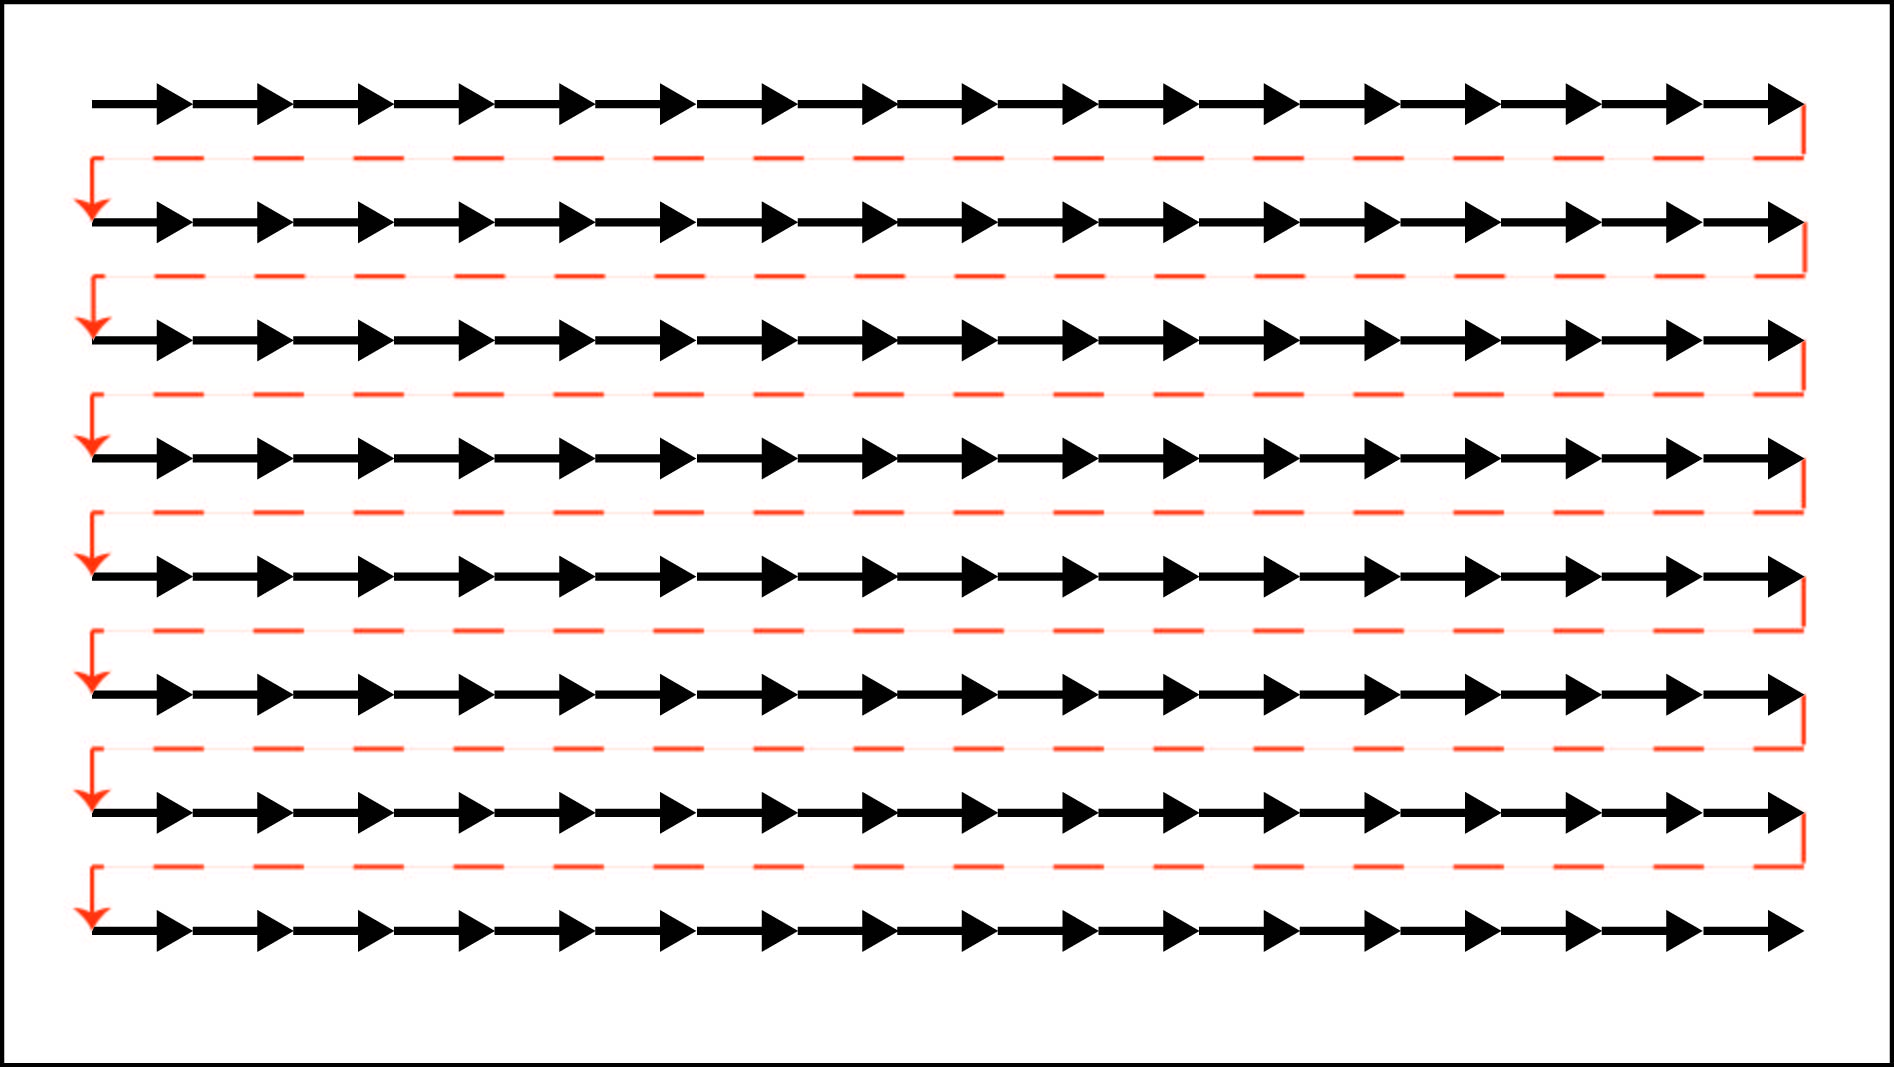
\includegraphics[width=12cm]{6_scanning.jpg}
	\caption{Proces skanowania -- schemat przemieszczania okna detekcji na obrazie}
	\label{fig:scan_scheme}
\end{figure}
Skanowanie obrazu $1280\times 720$ wymaga wykonania $7\cdot16=112$ iteracji algorytmu dla kolejnych nieparzystych klatek, co trwa nieco mniej niż 4 sekundy. 
Proces ten może trwać krócej, jeśli w jego trakcie osiągnie się bardzo dobry wynik klasyfikacji, poniżej zadanego poziomu \textit{SVM\_strong\_threshold}=$-1$; w standardowej procedurze wystarczy zapamiętany najlepszy wynik poniżej \textit{SVM\_threshold}=$-0.1$.

%TODO 2 Proszę jeszcze raz spokojnie ten podrozdział przeanalizować. Prostot, jak Steve Jobs. %ODP OK

\subsubsection{Weryfikacja pierwszej detekcji}

Kolejny etap, weryfikacyjny, jest uruchamiany bezpośrednio po zakończeniu skanowania i~polega na przeprowadzeniu 3 kolejnych iteracji SVM -- w trybie śledzenia (czyli na ograniczonym oknie, analizując obszar dla ostatniego wyniku SVM). 
Warunkiem przejścia przez ten etap jest, by wynik każdej iteracji był mniejszy od założonego maksimum \textit{SVM\_threshold}. 
W przeciwnym wypadku część PL przechodzi w stan bezczynności, ustawiana jest odpowiednia wartość statusu \textit{PL\_to\_PS\_status}, w odpowiedzi na którą część PS wyśle sygnał \textit{PS\_to\_PL\_run\_alg} rozpoczynający ponownie etap skanowania. 
Mechanizm ten stworzono, by kwestie decyzyjne związaną z dalszym postępowaniem przenieść do PS.


\subsubsection{Śledzenie}
Standardowe śledzenie opiera się na zweryfikowaniu wyniku ostatniej iteracji HOG+SVM, jednak proces uwzględnia jeszcze kilka elementów:
\begin{itemize}
	\item start algorytmu MeanShift -- wcześniej nieużywany algorytm MS ma możliwość rozpoczęcia pracy po zarejestrowaniu poprawnego wyniku klasyfikacji SVM (wartość mniejsza niż \textit{SVM\_strong\_threshold}). %TODO 2 czemu niedostępny - może nieużywany ? %ODP OK
	Wzorcem dla MS zostanie obszar z kolejnej klatki obrazu -- kwadrat o środku w $\{x,y-30\}$ -- gdzie $\{x,y\}$ to aktualny środek obszaru wyliczonego przez algorytm SVM. 
	Podane przesunięcie w pionie pozwala rozpocząć śledzenie MS na obszarze w obrębie klatki piersiowej, wartość dobrano empirycznie.
	
	\item wyłączenie algorytmu MeanShift -- MS może przesunąć obszar śledzenia poza śledzony obiekt, na przykład w związku ze zmianą oświetlenia. 
	By się przed tym ustrzec, konieczne jest wyłączenie algorytmu, by w stosownym momencie ponownie go uruchomić. 
	Odpowiedni warunek sprawdza, czy punkt MeanShift nie jest zbyt oddalony od punktu zwracanego przez poprawnie działający algorytm SVM.
	
	\item utrata śledzonego obiektu -- jeśli wynik ostatniej klasyfikacji nie spełnia \textit{SVM\_threshold}, może to oznaczać potencjalną utratę śledzonej postaci z pola widzenia. 
	Wówczas położenie osoby jest określane przez wynik działania algorytmu MeanShift, który stanowić będzie również wejście dla kolejnych iteracji HOG+SVM (poprawione o wspomniane wyżej przesunięcie $30$). 
	Warunkiem wyjścia z tego stanu (powrotu do standardowego śledzenia) jest osiągnięcie wyniku klasyfikacji rzędu \textit{SVM\_strong\_threshold}.
	Istotnym ograniczeniem jest wartość \textit{SVM\_lost\_iter}, która określa liczbę iteracji, w których ten tryb może pracować -- domyślnie są to ok. 3 sekundy (100 iteracji), jednak użytkownik może tę wartość modyfikować poprzez zapis do rejestru 0xC z poziomu konsoli. 
	Skala w~tym trybie nie jest aktualizowana -- ze względu na brak pozytywnych detekcji algorytmu HOG+SVM w śledzeniu wykorzystywana zostanie wartość skali z~ostatniego pozytywnego wyniku detekcji. %TODO to jest niejasne %ODP OK
	%TODO 2 to dalej jest niejasne. Co to znaczy, że ta skala jest zachowywana ? %ODP poprawiono
\end{itemize} 



Celem śledzenia jest utrzymanie obiektu w środku kadru. Sprowadza się to do ustalenia określonych wartości zadanych:
\begin{itemize}
	\item położenie punktu środkowego SVM: $\{x_{set},y_{set}\}=\{640,450\}$ 
	\item odległość kamery od osoby: $4$m, co umożliwia pozytywną detekcję dla określonej skali obrazu: $z_{set}=3$
\end{itemize}

Wartość $x_{set}$ jest dość oczywista i wyznacza dokładnie połowę szerokości kadru.
Wartość $y_{set}$ została dobrana eksperymentalnie i jest związana potrzebą utrzymania odpowiedniej wysokości przez drona -- ok $1.5$m (zależnie od skali).
Ostatecznie, dla skal użytych w projekcie: $2/2.5/3/3.5/4$, dobór $z_{set}=3$ jest najbardziej rozsądny ze względu szacowaną odległość postaci od drona -- $4$m -- oraz możliwość detekcji postaci w bliższej oraz dalszej odległości.

Uchyb regulacji jest wyznaczany po każdej iteracji algorytmu SVM. 
Opiera się na obliczeniu różnicy pomiędzy obecnymi koordynatami SVM, a ustalonymi wartościami zadanymi.
Ponadto, w przypadku skali zdecydowano, by obliczana była średnia krocząca 4 ostatnich wyników poprzez ich zsumowanie, a następnie przesunięcie bitowe o 2 w prawo, równe dzieleniu przez 4.
Taki zestaw danych jest co określoną liczbę iteracji (domyślnie 15, czyli $0.5$s) przepisywany do rejestru 0x04 do którego dostęp ma część PS. Flaga \textit{PL\_to\_PS\_control} ustawiana wówczas w sygnale GPIO wywołuje obsługę przerwania, skutkującego ruchem drona. 
Częstotliwość wysyłania takiego sygnału można konfigurować rejestrem \textit{SVM\_iter\_between\_control}.


\subsection{Komunikacja Zynq <-> autopilot} 

Wymiana informacji pomiędzy autopilotem, a układem SoC bazuje na transmisji UART o~standardowej prędkości równej 115200 bodów. 
Za transmisję po stronie układu SoC jest odpowiedzialna część PS, jednak istnieje możliwość lokalizacji sygnałów RxD oraz TxD po stronie części PL (wybór spośród większej liczby pinów) \cite{PYNQ_sch}. 
Z kolei w~autopilocie skonfigurowano port TELEM 2 \cite{PixhawkSerial}. 
Warstwą transportową jest protokół MAVLink, który opisano w~dodatku \ref{subsec:MAVLink}

Został on zaprojektowany w postaci plików nagłówkowych -- taka forma umożliwia łatwe wykorzystanie w aplikacji tworzonej na jeden z rdzeni procesora ARM dostępnego na SoC Zynq. 
Ponadto, każda z dostępnych wiadomości ma swój podzbiór funkcji umożliwiających proste pakowanie w zestaw bajtów lub poprawne sparsowanie odebranych informacji.


\subsubsection{Aplikacja uruchomiona na procesorze ARM układu SoC Zynq}

O ile część PL układu Zynq jest tworzona w środowisku Xilinx Vivado, to narzędziem deweloperskim obsługującym PS jest inny program będący częścią pakietu firmy Xilinx -- SDK (Software Development Kit). 
By jednak możliwe było rozpoczęcie pracy, konieczne jest zaimportowanie z Vivado tzw. konfiguracji sprzętowej, czyli informacji o dostępnych w PS peryferiach, oraz połączeniach pomiędzy PS a PL.

Jednym z nich jest GPIO, do którego podłączony został sygnał \textit{trigger\char`_algorithm}, status algorytmów oraz wartości uchybu regulacji. 
Odpowiednio skonfigurowane GPIO może generować przerwania, co wykorzystano jako reakcję na zmianę stanu któregokolwiek z opisanych wyżej sygnałów.

Pozostałymi peryferiami są dwa interfejsy UART. 
Lokalizacją dla pierwszego interfejsu UART są dwa piny, które połączono z odpowiednim portem autopilota. 
Aplikacja, korzystając z biblioteki MAVLink, jest w stanie zdekodować i sparsować ramki przychodzące oraz odpowiednio spakować komendy wysyłane do autopilota.

Drugi interfejs UART, wyprowadzony domyślnie na wyjście microUSB płyty PYNQ, stanowi połączenie z komputerem jako element różnorakich testów i debugowania w trakcie implementacji. 
Utworzono dla niego prostą formę terminala, który w odpowiedzi na komendy wpisywane z klawiatury komputera umożliwia zapis i odczyt z rejestrów testowych, wysyłanie określonych wiadomości do autopilota, ale przede wszystkim wyświetla odpowiednio sparsowane informacje wysyłane przez autopilot.

W aplikacji zaimplementowano nadrzędną maszynę stanu, której częstotliwość pracy jest nadana przez odbierane co sekundę wiadomości z autopilota o ID=0, które noszą nazwę „HEARTBEAT”.
Odpowiada ona za przygotowanie maszyny do śledzenia: uzbrojenie (komenda ARM), start (komenda TAKEOFF) i odczekanie określonego czasu przed rozpoczęciem skanowania. Wysłanie nowej komendy ruchu w trakcie etapu śledzenia jest realizowane niezależnie  podczas obsługi przerwania związanego z GPIO, po otrzymaniu sygnału \textit{PL\_to\_PS\_control}. 
Wykorzystywana jest w tym celu komenda SET\_POSITION\_TARGET\_LOCAL\_NED, której opis znajduje się w dodatku \ref{commands}. 
Warto zaznaczyć, że o ile oprogramowanie autopilota ArduCopter wyróżnia 14 trybów lotu drona, to trybem, który realizuje komendy ruchu wysyłane protokołem MAVLink, jest tryb GUIDED. 
Zostało to szerzej opisane w dodatku \ref{flightmodes}.


Podstawowym warunkiem pracy maszyny stanu jest obecność sygnału \textit{trigger\char`_algorithm}. 
Po jego zboczu narastającym następuje próba uzbrojenia drona; po zmianie stanu sygnału na niski (zmiana stanu przełącznika aparatury radiowej) procesor wyśle komendę rozpoczynającą proces lądowania. 
Bardziej szczegółowy opis komunikacji z dronem przedstawia schemat \ref{fig:PL_FSM_sch}.
Ostatecznie, przesunięcia dla każdej osi są obliczane według wzorów realizujących regulator proporcjonalny:
\begin{equation}
\left.\begin{aligned}
x_{mov}&= \frac{\boldmath{z_{set}}-z_{new}}{x_w}\\
y_{mov}&= \frac{x_{new}-\boldmath{x_{set}}}{z_{new}\cdot y_w}\\
z_{mov}&= \frac{y_{new}-\boldmath{y_{set}}}{z_{new}\cdot z_w},\\
\end{aligned}\right.
\end{equation}
gdzie: $y_{new}$, $x_{new}$, $z_{new}$ to informacje pochodzące z algorytmów MS/HOG+SVM, a \textit{$x_w$, $y_w$, $z_w$} są empirycznie dobranymi współczynnikami dopasowującymi wartości do jednostek. 
Nie bez znaczenia jest także skojarzona z wynikiem detekcji skala obrazu -- dla mniejszych skal (obiekt dalej od kamery) potrzebny jest większy ruch drona. 
%TODO 2 czyli regulator proporcjonalny ? by wychodził z tego. W future work dopisać prace nad bardziej lepiej regulatorem. %ODP OK
Warto zwrócić uwagę na zmianę osi układu współrzędnych drona:
\begin{itemize}
	\item \textit{x} -- oś pozioma odpowiadająca kierunkowi ruchu statku powietrznego (aspekt głębokości na obrazie),
	\item \textit{y} -- oś pozioma prostopadła do osi \textit{x},
	\item \textit{z} -- oś pionowa, zwrócona w dół.
\end{itemize}

\begin{figure}[ht]
	\centering
	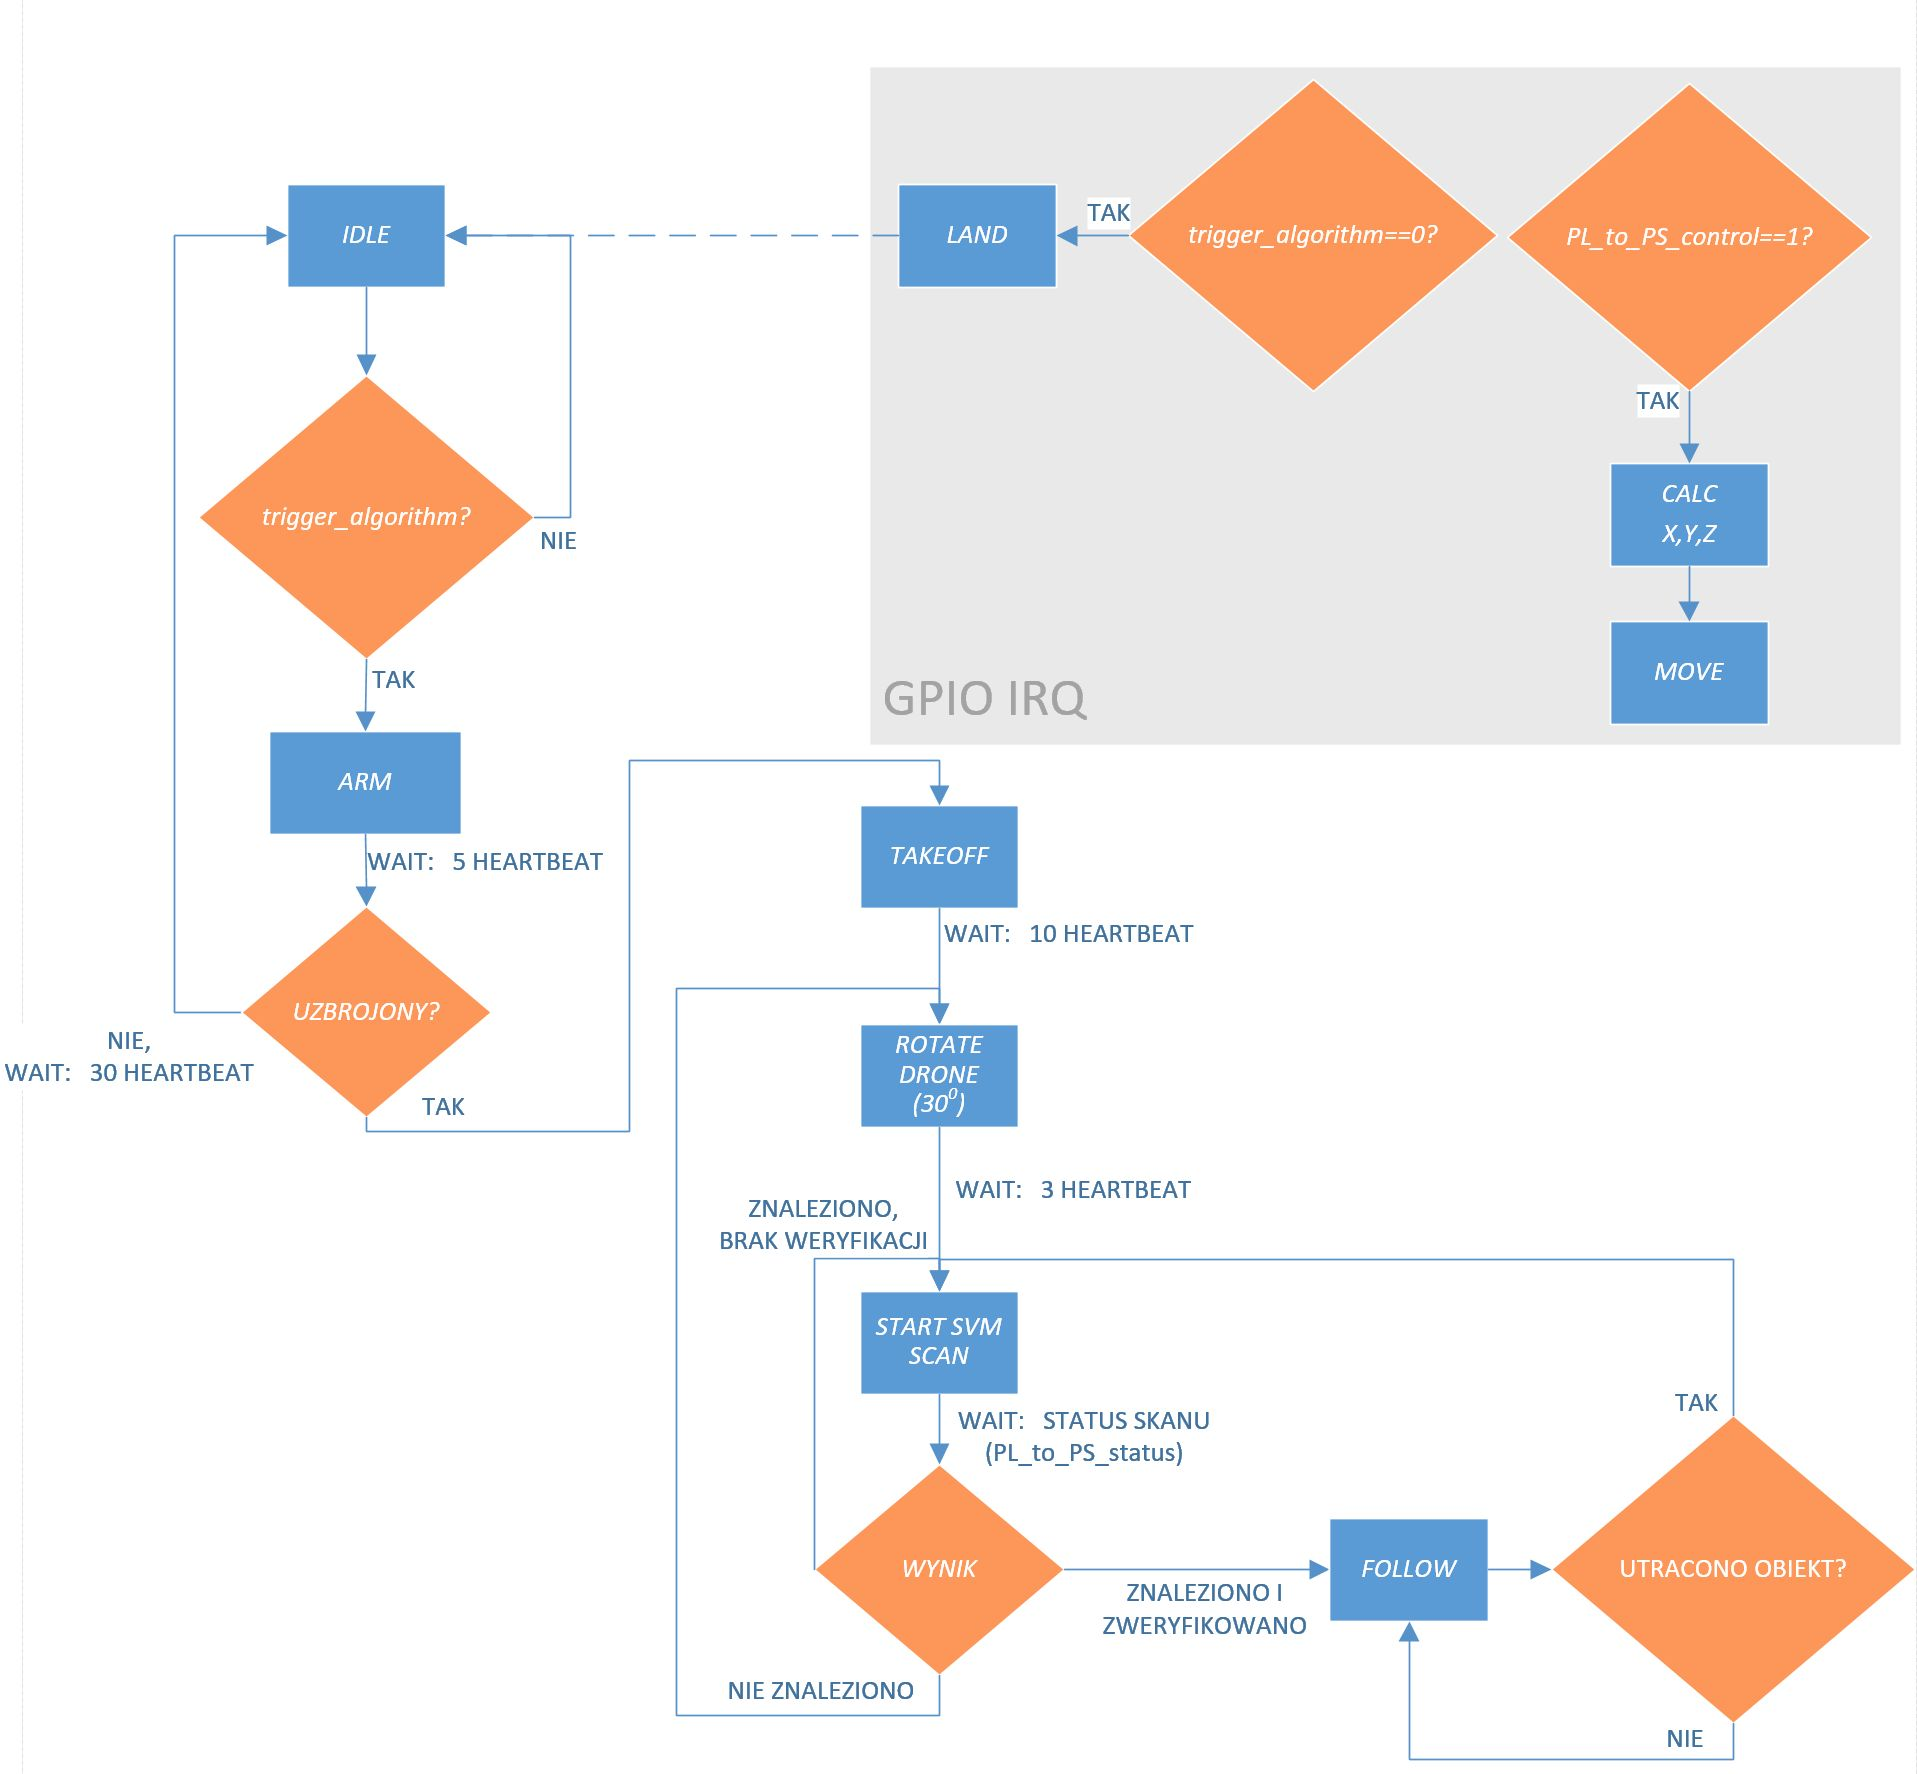
\includegraphics[width=16cm]{5_PS_FSM.jpg}
	\caption{Schemat działania aplikacji w PS}
	\label{fig:PL_FSM_sch}
\end{figure}

Domyślnie, maszyna stanu znajduje się w trybie bezczynności i oczekuje na pojawienie się sygnału \textit{trigger\char`_algorithm}. 
Wówczas podejmowana jest próba uzbrojenia z czasem oczekiwania -- 5 sekund. 
Autopilot wykonuje wtedy serię pomiarów weryfikacyjnych. 
Często ma jednak miejsce sytuacja, w której dron nie zostanie uzbrojony np. w wyniku otrzymania niedokładnych pomiarów GPS. 
Jeśli proces ten się nie powiódł (informacja o stanie drona jest przesyłana z wiadomością HEARTBEAT), mija kolejne 30 sekund, i ponawiana jest próba uzbrojenia -- do skutku. %TODO 2 a jak ta się nie powiedzie ? %ODP OK
Pomyślny przebieg procedury uzbrojenia pozwala wysłać komendę TAKEOFF z~parametrem określającym docelową wysokość drona -- $2$m. %TODO 2 inaczej zacząc, bo dziwnie się łączy z poprzednim zdaniem. Jaka wysokość ? %ODP OK
Po kolejnych 10 sekundach dron potwierdza responsywność, obracając się o 30 stopni zgodnie z ruchem wskazówek zegara i po 3 sekundach rozpoczyna proces skanowania. 
PS jest informowane o stanie tego procesu poprzez sygnał \textit{PL\_to\_PS\_status} -- w oparciu o aktualizację jego wartości maszyna stanu wymusza obrót urządzenia i nowe skanowanie (brak detekcji) powtórzenie skanowania dla obecnej orientacji (brak weryfikacji) lub przechodzi do trybu śledzenia. 
W maszynie stanu ten etap został on zrealizowany dość pasywnie, bowiem analizuje jedynie stan detekcji i w przypadku permanentnej utraty obiektu z pola widzenia następuje powrót do procedury skanowania. 
Za wydawanie komend ruchu odpowiada funkcja obsługi przerwania GPIO, która jest uruchamiana po każdej zmianie tego sygnału.


\section{Podsumowanie stworzonej architektury}

Ostatecznie architekturę programowo-sprzętową może przedstawić schemat \ref{fig:5_top_scheme}, opisujący najważniejsze zależności pomiędzy modułami. 
Zauważyć można podobieństwo sygnałów związanych z implementacją poszczególnych algorytmów -- upraszcza to ich integrację w module TOP\_LAYER.

\begin{figure}[ht]
	\centering
	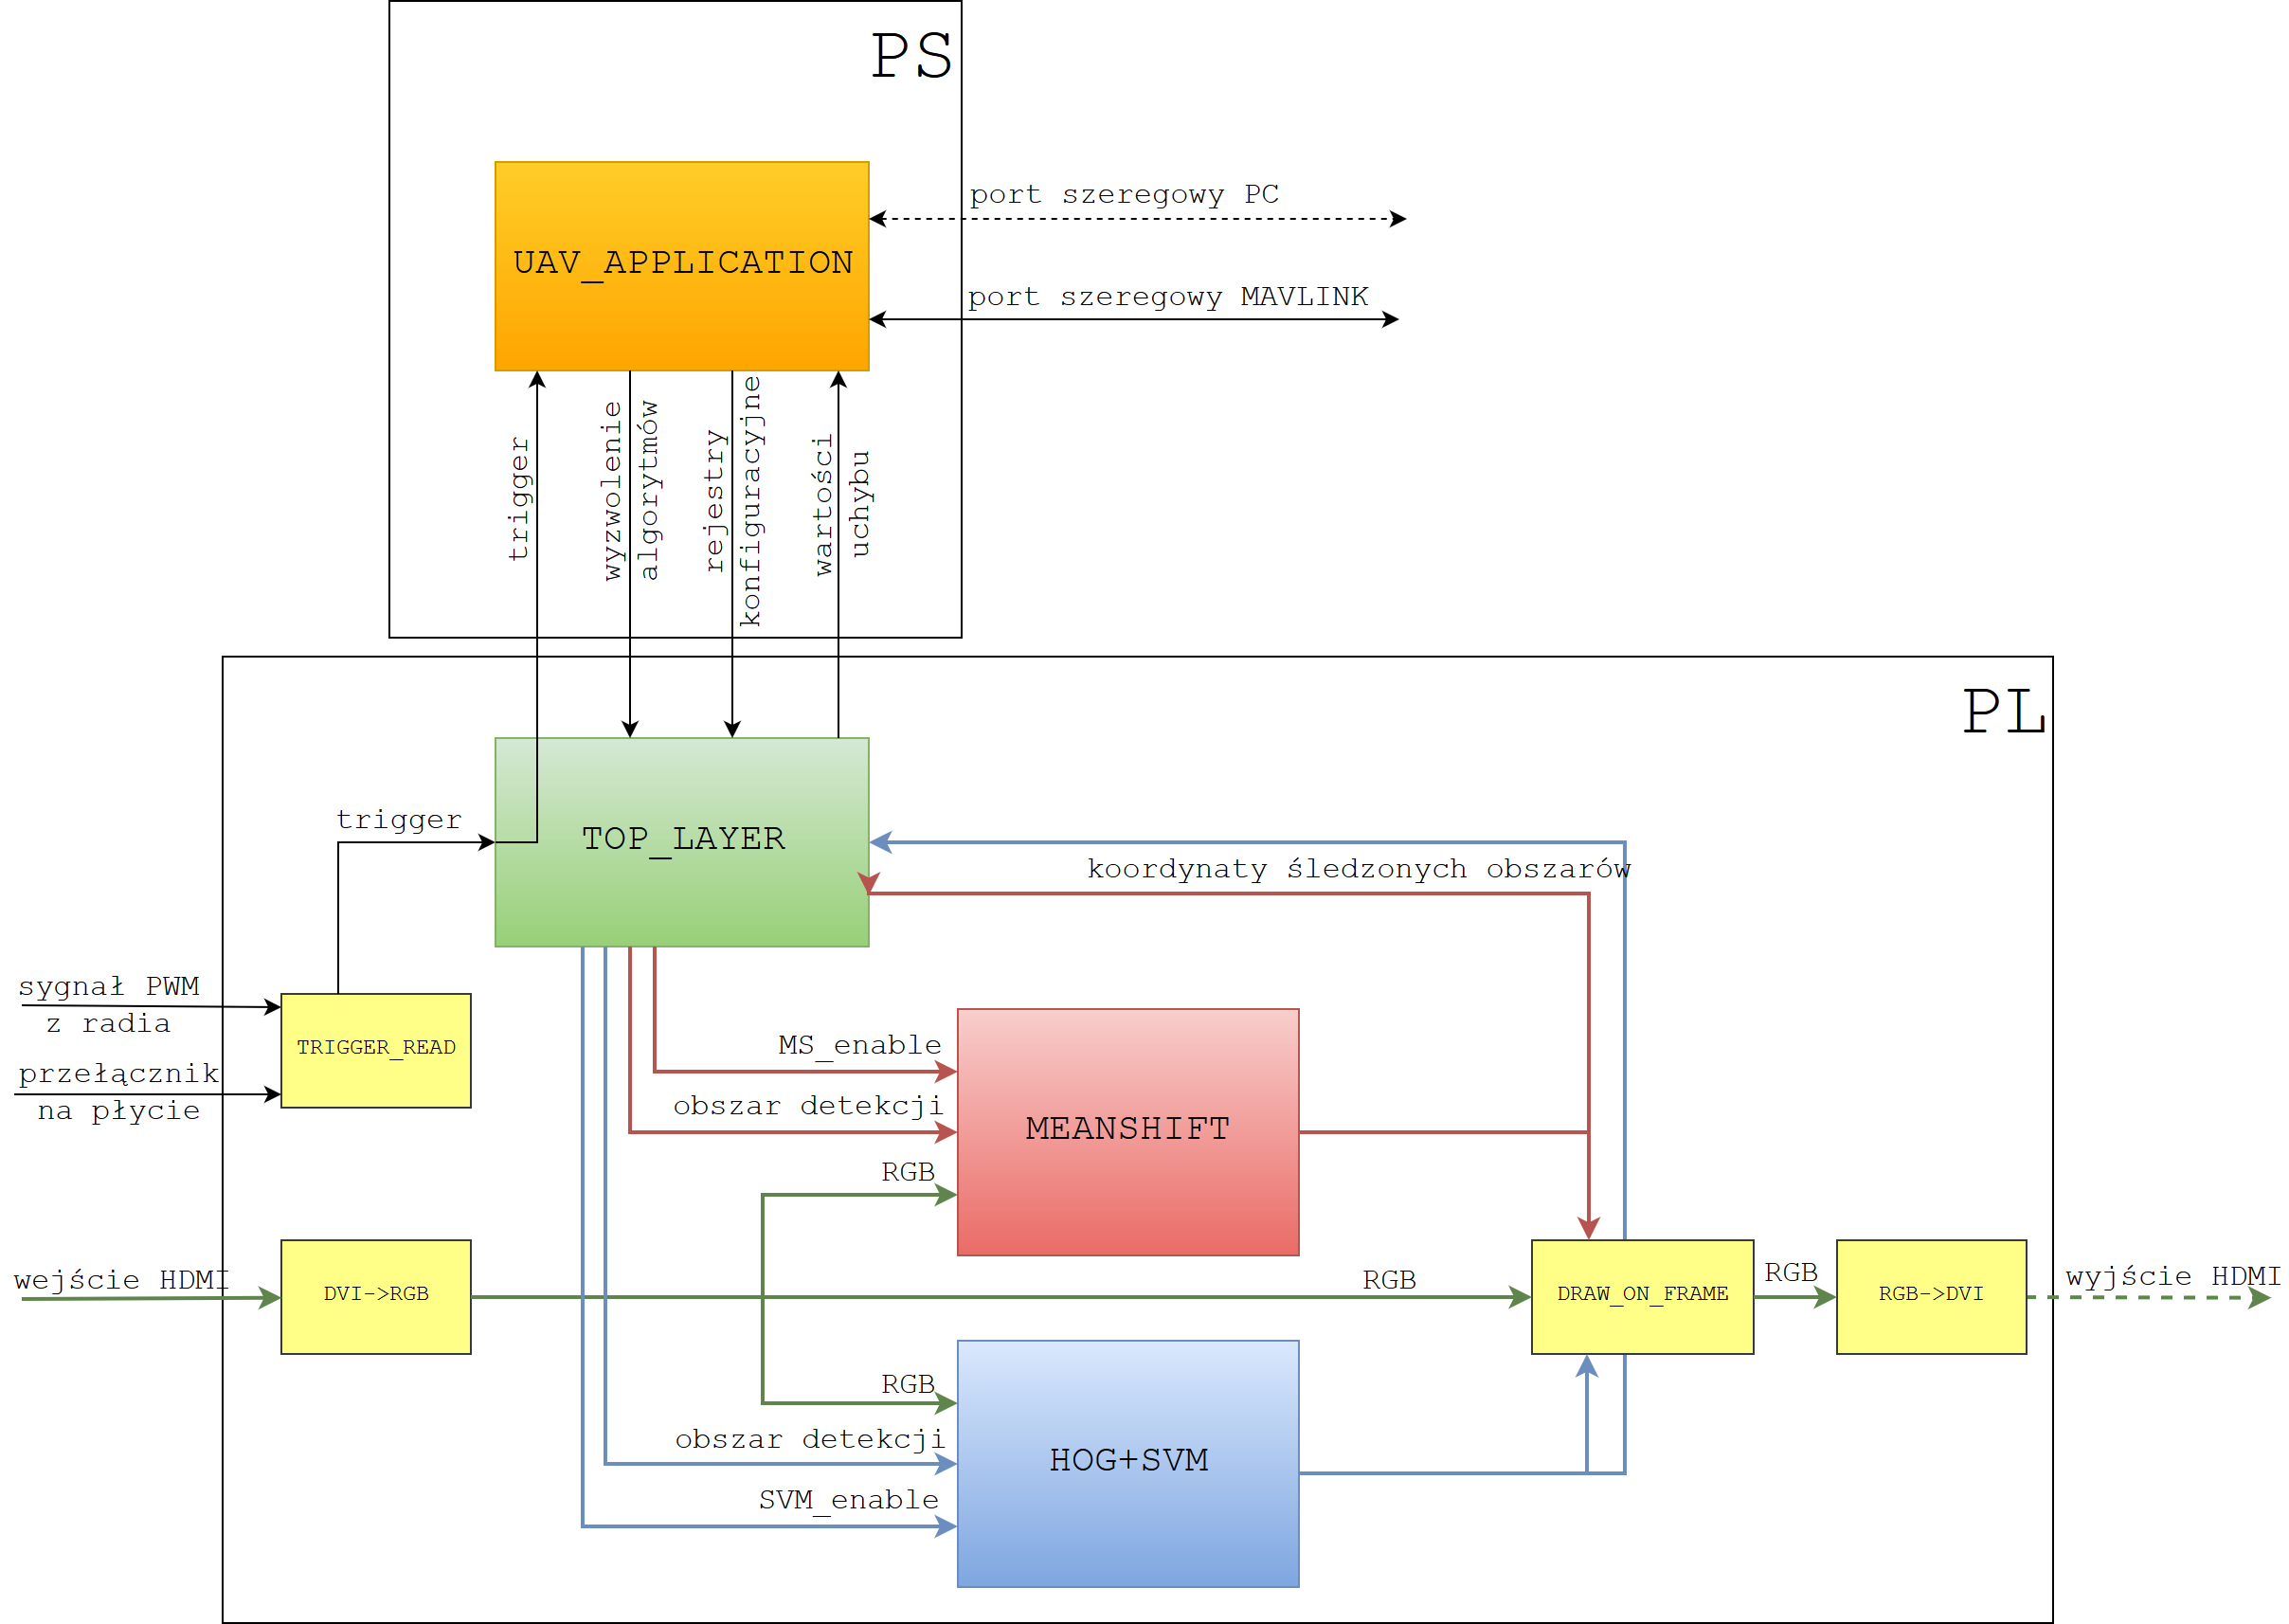
\includegraphics[width=16cm]{hardware_algorithm.png}
	\caption{Schemat architektury programowo-sprzętowej}
	\label{fig:5_top_scheme}
\end{figure}

Proces implementacji sprzętowej wymagał systematycznego nadzoru wykorzystania zasobów w układzie. %TODO 2 styl. to szedł w parze... %ODP OK
Zbyt mała ilość dostępnych w logice elementów mogłaby mieć wpływ na rozmieszczenie (ang. \textit{routing}) sygnałów i problemy związane z czasami ich ustalania lub podtrzymania (ang. \textit{setup/hold time}). 
Tabele \ref{tab:utilizationMS}, \ref{tab:utilizationHOG} oraz \ref{tab:utilizationOverall} przedstawiają wykorzystanie zasobów w układzie Zynq 7Z020. Informacje te pozwalają wnioskować, że plany dalszego rozwoju systemu nie muszą wiązać się ze zmianą układu na większy. Jest to jednak aspekt, do którego należy podejść z rozwagą, mając na uwadze wymagania związane z odpowiednim rozmieszczeniem logiki w układzie. Z kolei bezpośrednie porównanie implementacji algorytmów MeanShift i HOG+SVM ukazuje znaczną dysproporcję w wykorzystaniu zasobów. Najbardziej trafnym uzasadnieniem może tu być fakt realizacji algorytmu HOG+SVM na pięciu skalach, które w uproszczeniu można potraktować jak 5 odrębnych instancji algorytmu.

%TODO 2 nie zaszkodziłoby kilka zdań komentarza do tabelek.%ODP OK
\begin{table}[ht]
	\centering
	\caption{Wykorzystanie zasobów dla implementacji algorytmu MeanShift}
	\captionsetup{justification=centering,margin=1cm}
	\begin{tabular}{|P{3cm} |P{3cm} |P{3cm}|P{4cm}|}	
		\hline
		\rowcolor{lightgray} Rodzaj zasobu & Wykorzystane & Dostępne & Wykorzystanie [\%]\\ 
		LUT		& 5255	& 53200 & 9.8\\ 
		\hline
		FF		& 8562	& 106400 & 8.0\\ 
		\hline
		BRAM	& 25.5	& 140 & 18.2\\ 
		\hline
		DSP		& 28	& 220 & 12.7\\ 
		\hline		
	\end{tabular}

	\label{tab:utilizationMS}
\end{table}

\begin{table}[ht]
	\centering
	\caption{Wykorzystanie zasobów dla implementacji algorytmu HOG+SVM}
	\captionsetup{justification=centering,margin=1cm}
	\begin{tabular}{|P{3cm} |P{3cm} |P{3cm}|P{4cm}|}	
		\hline
		\rowcolor{lightgray} Rodzaj zasobu & Wykorzystane & Dostępne & Wykorzystanie [\%]\\ 
		LUT		& 23894	& 53200 & 44.9\\ 
		\hline
		FF		& 32668	& 106400 & 30.7\\ 
		\hline
		BRAM	& 66	& 140 & 47.1\\ 
		\hline
		DSP		& 55	& 220 & 25\\ 
		\hline		
	\end{tabular}
	\label{tab:utilizationHOG}
\end{table}

\begin{table}[ht]
	\centering
	\caption{Wykorzystanie zasobów - pełna architektura}	
	\captionsetup{justification=centering,margin=1cm}
	\begin{tabular}{|P{3cm} |P{3cm} |P{3cm}|P{4cm}|}	
		\hline
		\rowcolor{lightgray} Rodzaj zasobu & Wykorzystane & Dostępne & Wykorzystanie [\%]\\ 
		LUT		& 33729	& 53200 & 63.4\\ 
		\hline
		FF		& 46385	& 106400 & 43.6\\ 
		\hline
		BRAM	& 92	& 140 & 65.7\\ 
		\hline
		DSP		& 83	& 220 & 37.7\\ 
		\hline		
	\end{tabular}
	\label{tab:utilizationOverall}
\end{table} 

Dodatkowo, postanowiono dokonać estymacji poboru mocy przez układ. 
W tym celu w środowisku Vivado wygenerowano raport w oparciu o określenie temperatury otoczenia równej $25^{\circ}$C i wybór najbardziej pesymistycznego poziomu estymacji. 
Z dokumentu wynika, że całkowity pobór mocy w układzie nie powinien przekraczać $3.5$W, z czego jednak aż $1.3$W to wartość pobierana przez część PS. 
Fragment logiki realizujący metodę HOG+SVM potrzebuje $0.99$W, natomiast MeanShift zaledwie $0.11$W.
\chapter{Integracja układu FPGA z dronem}

Opisana w poprzednim rozdziale architektura sprzętowa dotyczyła dwóch algorytmów, które mogą funkcjonować niezależnie od siebie. 
Ostatecznie jednak istnieje jeszcze najwyższa warstwa logiczna, która pozwala wykorzystać je jak najlepiej, oraz odpowiada za komunikację z dronem.
%TODO do rozbudowy, ale w kontekście zawartości 'nowego" rozdziału początkowego.


\subsection{Autopilot}

Każdy dron byłby bezużyteczną konstrukcją, gdyby nie serce maszyny -- tzw. autopilot. 
W tym przypadku postanowiono wykorzystać urządzenie Pixhawk. 
Jest to zgodny ze standardami przemysłowymi moduł na otwartej licencji, stworzony przy współpracy z firmą 3D Robotics oraz ArduPilot Group. 
Posiada następujące parametry:
\begin{itemize}
	\item procesor Cortex-M4F taktowany zegarem 168 MHz,
	\item sensory: trzyosiowy akcelerometr, żyroskop, kompas magnetyczny, barometr i zewnętrzny GPS,
	\item slot na kartę microSD,
	\item możliwość połączenia peryferiów (interfejsy: UART, I2C, CAN),
	\item 14 wyjść PWM (8 głównych z zabezpieczeniami + 6 dodatkowych).
\end{itemize}

\begin{figure}[h]
	\centering
	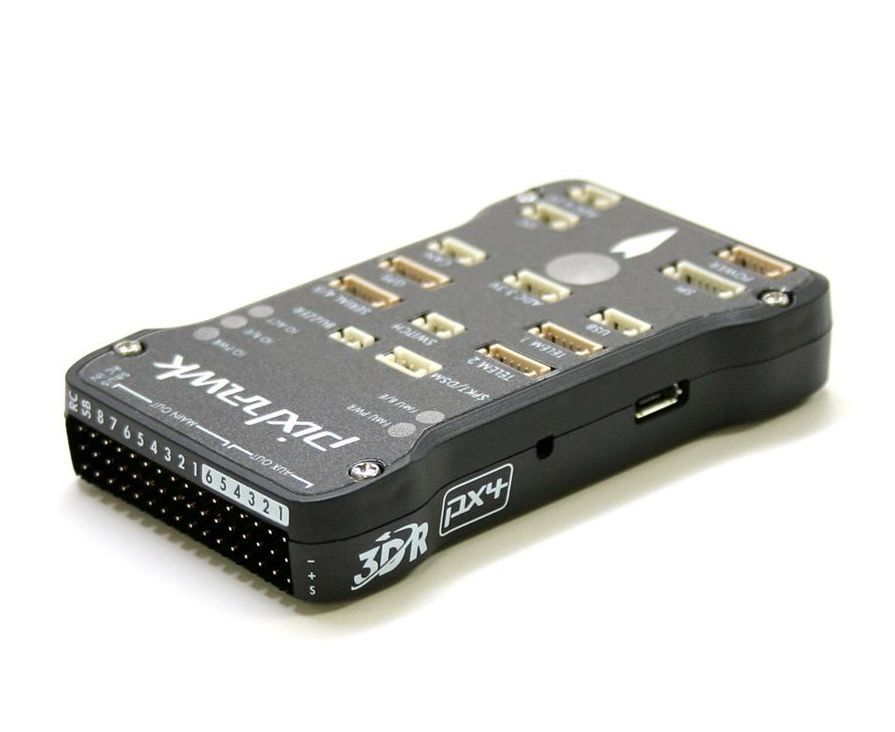
\includegraphics[width=8cm]{5_pixhawk.jpg}
	\caption{Autopilot Pixhawk -- widok na panel główny oraz we/wy PWM}
	\label{fig:pixhawk}
\end{figure}

Powyższy sprzęt jednak nie jest w pełni skonfigurowany do pracy po wyjęciu z pudełka -- szczególnie, że jako produkt uniwersalny, bywa montowany na konstrukcjach o szerokim rozrzucie parametrów. 
Może zapewnić sterowanie śmigłowcom (tzw. multicopterom), samolotom modelarskim oraz nawet łazikom. %TODO mam wątpliwość, czy słowo "kopter" jest poprawne. Skoro helikopter jest niepoprawny (był taki słynny przetarg..) to trzeba śmigłowiec. %ODP OK, do nawiasu wrzucono potoczną nazwę.
W przypadku dwóch pierwszych grup konfiguracja wiąże się ze zdefiniowaniem odpowiedniej liczby śmigieł i ich rozstawienia, typu aparatury radiowej oraz zewnętrznych urządzeń geolokalizacyjnych. 
Tę dość dużą elastyczność mogą zapewnić dwa główne systemy, które są wczytywane z pamięci SD i pracują w czasie rzeczywistym. 
Dedykowany, PX4 Flight Stack jest stworzony przez twórców modułu, oraz ArduPilot Copter (ArduCopter) -- niezależny, otwarty system, który został dostosowany do platformy Pixhawk z wykorzystaniem dostępnych narzędzi deweloperskich. 
Ze względu na większą bazę użytkowników i dojrzałość projektu, wybrano drugie rozwiązanie.

\begin{figure}[h]
	\centering
	\captionsetup{justification=centering,margin=1cm}
	\hspace*{0cm}
	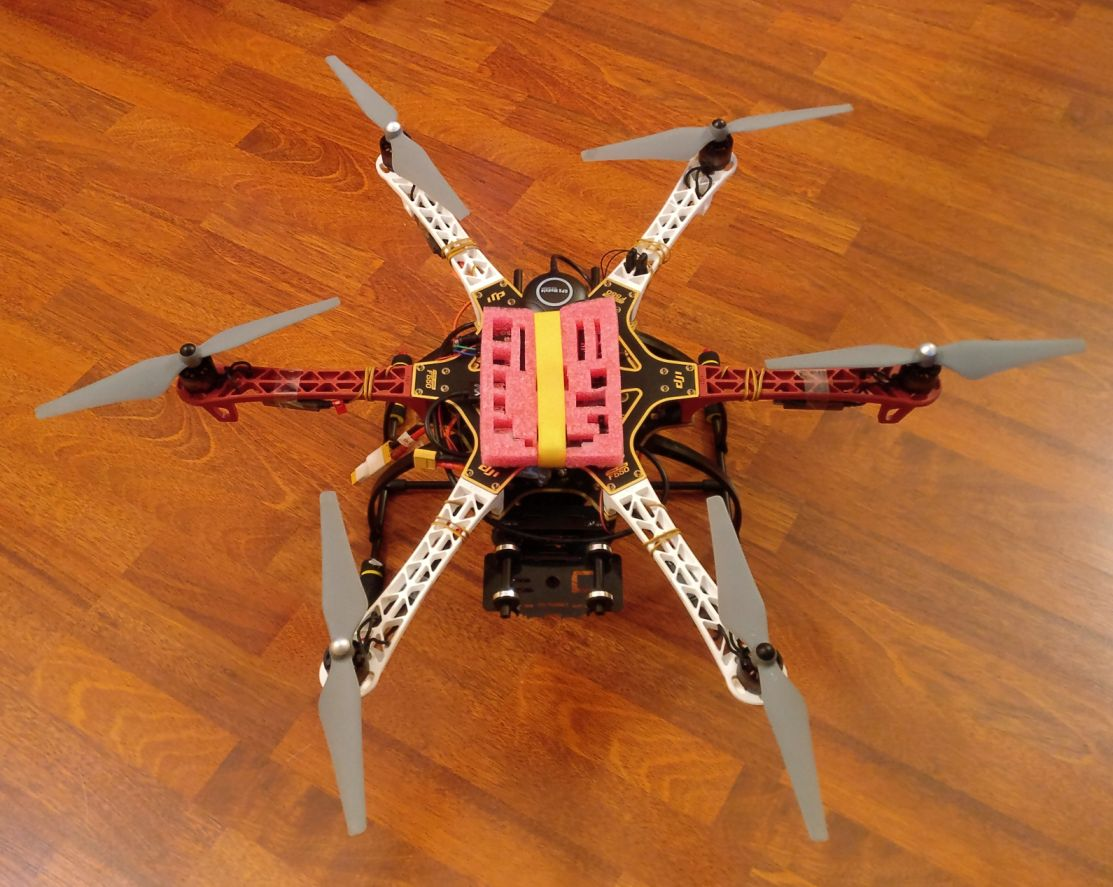
\includegraphics[width=14cm]{5_drone_photo.jpg}
	\caption{Zdjęcie przedstawiające w pełni wyposażonego drona. Pod gąbką ochronną skrywa się układ PYNQ}
	\label{fig:drone_photo}
\end{figure}
%TODO Brak referencji w txt. "skrywa" się potoczne.

\subsection{Propagacja sygnałów} %TODO średni tytuł

Zbudowanie drona w oparciu o gotowe komponenty nie jest zadaniem skomplikowanym. 
Jednak z uwagi na wymagania projektu zapewniające jego autonomizację, należało dokładnie przemyśleć jego przebudowę. %TODO przerobić zdanie, że z uwagi na wymagania projektu - które powinny być opisane wcześniej. %ODP OK
Schemat \ref{fig:architecture} przedstawia architekturę sygnałową. %TODO arch. sygnałową - dziwne określenie
\begin{figure}[]
	\centering
	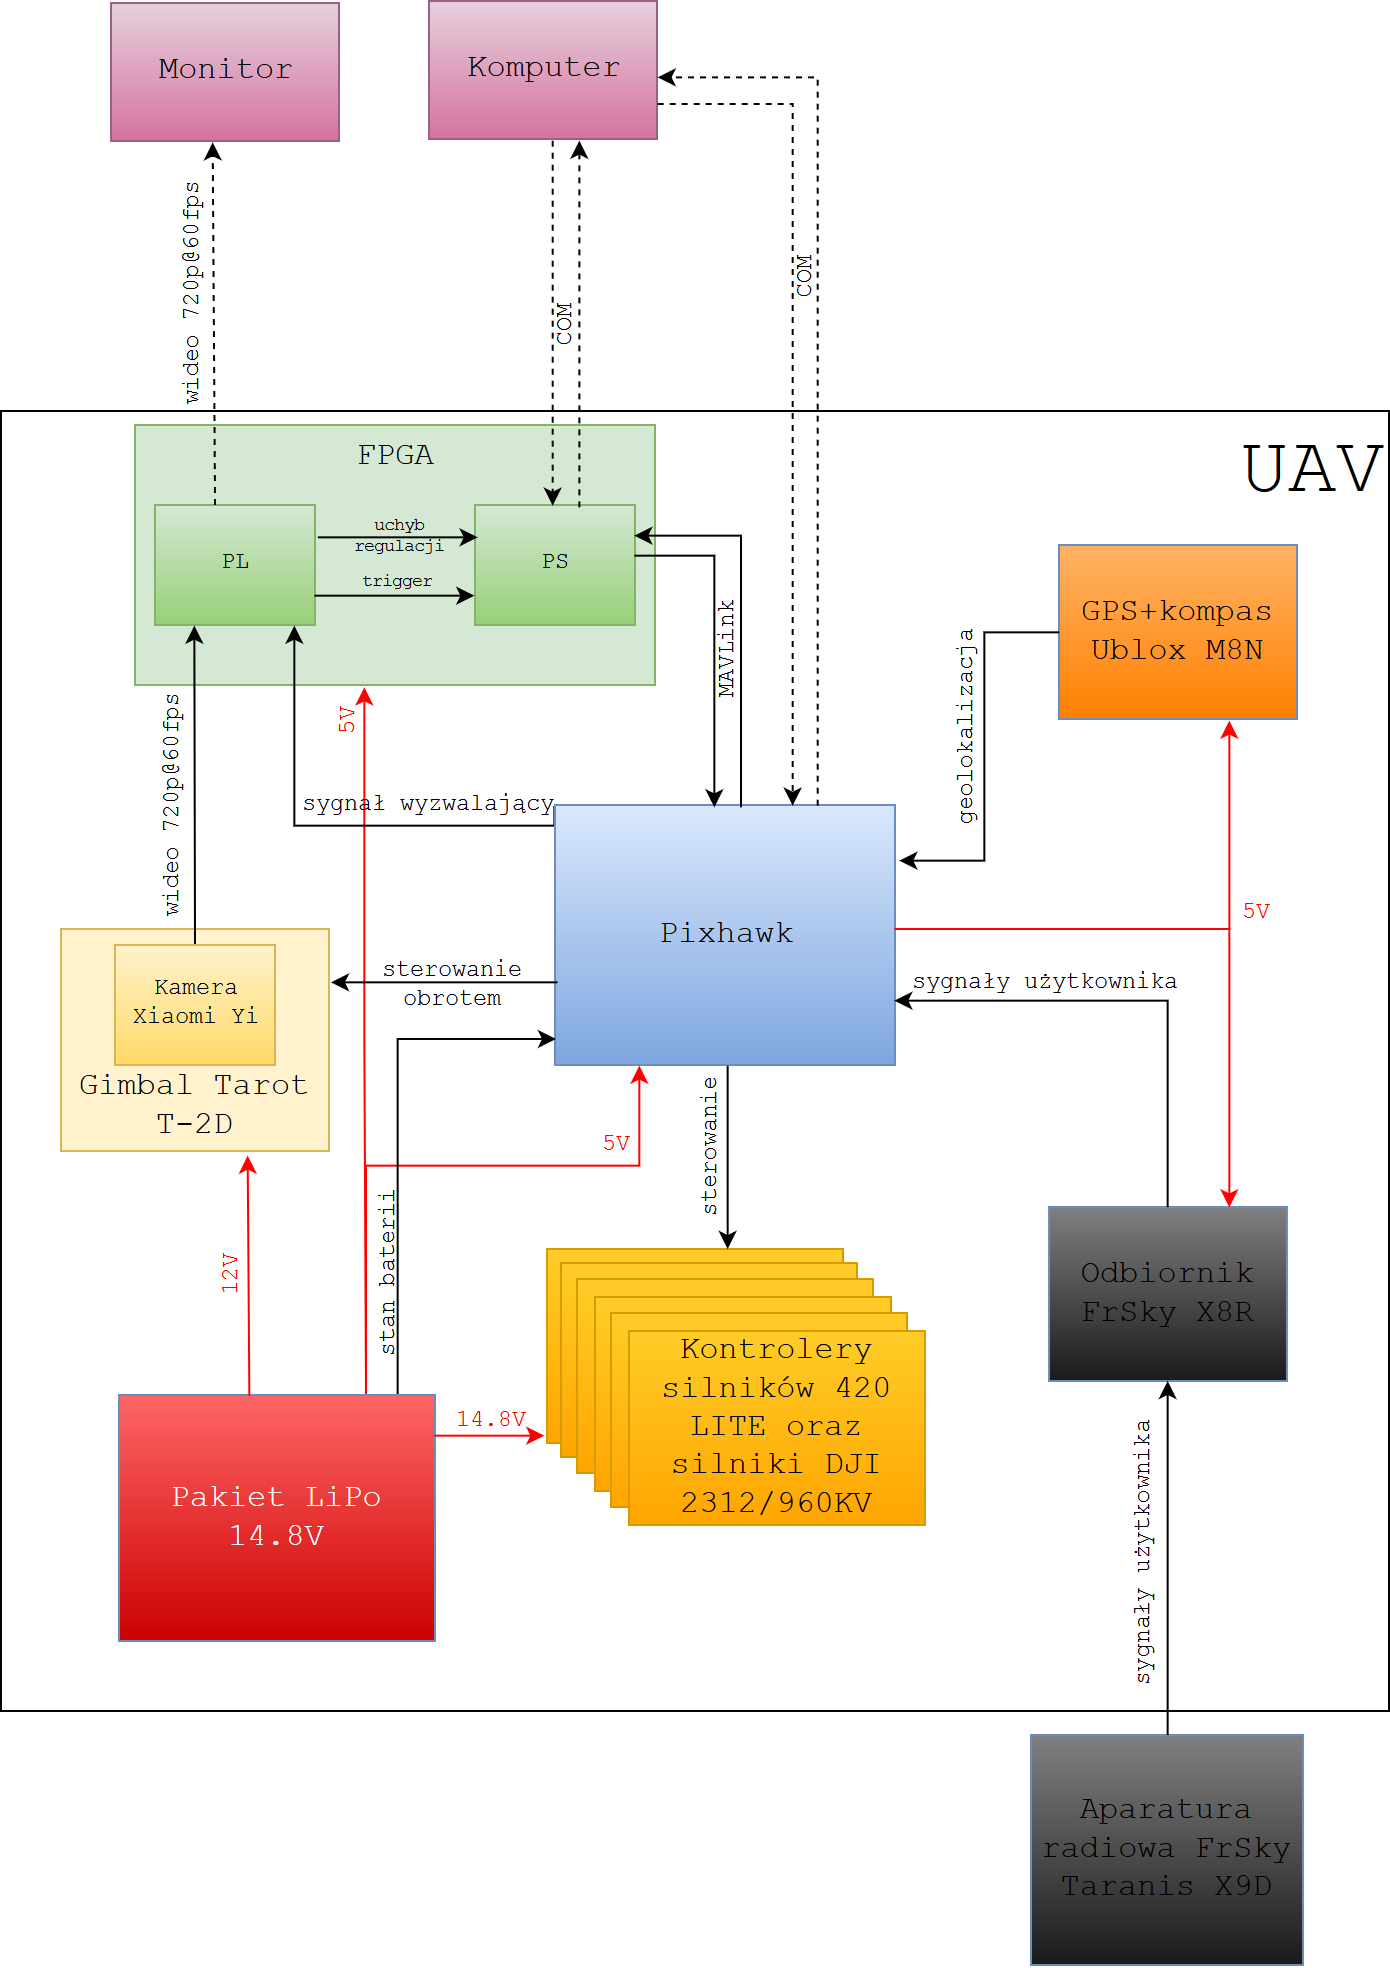
\includegraphics[width=14cm]{5_drone_architecture.png}
	\caption{Architektura sygnałowa tworzonego projektu}
	\label{fig:architecture}
\end{figure}

%TODO brakuje omówienia rysunku. Trzeba go po prostu opisać w tekście.
%TODO co to znaczy komputer w trakcie implementacji ?


\section{Zdalne uruchomienie pracy systemu}

%TODO To już może być treść tego rozdziału. Tylko oczywiście po jakimś wstępie.

Początkowo stworzono (i ostatecznie pozostawiono) możliwość rozpoczęcia pracy z wykorzystaniem jednego z przełączników na płycie PYNQ, gdyż prace nad projektem wymagały dość częstego uruchamiania algorytmu jeszcze bez udziału drona. 
Jednak lot maszyny lub nawet jego start praktycznie wyklucza fizyczny dostęp do układu FPGA, dlatego koniecznością stało się zdalne wyzwolenie pracy algorytmów. 
Sygnał wyzwalający nosi nazwę \textit{trigger\char`_algorithm}.

Podczas lotu maszyny użytkownik ma pod ręką jedynie aparaturę radiową, z poziomu której może jednak w dość prosty sposób wysyłać sygnały . %TODO wystawiać - potoczne %ODP OK
Aparatura jest bowiem wyposażona w szereg konfigurowalnych przełączników analogowych i cyfrowych. 
Ponadto, dane są wysyłane poprzez 16 kanałów -- przy czym do kontroli podstawowych funkcji drona wykorzystuje się zaledwie 4. %TODO raczej nie 16 kanałów tylko przez / poprzez... %ODP OK
Wybrano zatem jeden z pozostałych dostępnych kanałów, któremu przypisano funkcję trzypoziomowego przełącznika obecnego na panelu urządzenia radiowego.

Sparowany z aparaturą odbiornik, który jest zamocowany na dronie, wysyła wszystkie dane po jednym zestawie przewodów w formie PPM (ang. \textit{Pulse Position Modulation}). %TODO napisać, że odbiornik jest na dronie %ODP OK
Taki sygnał musiałby być zdekodowany w części PL układu Zynq do uzyskania użytecznej wartości. %TODO nie nie FPGA.. Zynq/lb PL %ODP OK
Proces dekodowania rozwiązuje jednak autopilot, który konwertuje 16-kanałowy PPM na znacznie prostsze sygnały PWM (ang. \textit{Pulse Width Modulation}) m.in. do kontroli silników. %TODO wystawia %ODP OK
Co więcej, Pixhawk umożliwia przypisanie reszty kanałów transmisyjnych do pomocniczych wyjść PWM. 
Rozwiązanie to znalazło zastosowanie chociażby w ustawieniu wartości zadanych serwomechanizmom odpowiedzialnym za pracę gimbala kamery.

%Ostatecznie, postanowiono ustalić warunki kwestią niejasną pozostała szerokość pulsu, który miałby wyzwolić działanie algorytmu. %TODO dalczego niejasną ? %ODP rozpisano się na ten temat poniżej
Za pomocą oprogramowania Mission Planner, służącego do konfiguracji autopilota, ustawiono zakres szerokości wysyłanego pulsu PWM na $1100-1900$us. Wybranie odpowiedniej wartości wyzwalającej pracę systemu wymagało dodatkowej weryfikacji, która uwzględniałaby przypadek z wyłączoną aparaturą radiową (brak wejściowego sygnału PPM) i ewentualne błędy w transmisji PWM.
Do pomiarów zastosowano analizator logiczny ILA wbudowany w środowisko Vivado i stworzono prosty licznik, który jest poddawany następującym operacjom:
%TODO na którym - styl i po co to ILA - do pomiarów. %ODP OK
\begin{itemize}
	\item kasowanie na zboczu narastającym sygnału wejściowego,
	\item inkrementację podczas aktywnego stanu sygnału,
	\item przypisanie tej samej wartości w każdym innym przypadku.
\end{itemize}

Logika jest taktowana zegarem \textit{calc\char`_clk} $=100$MHz i dla poszczególnych pozycji przełącznika na aparaturze radiowej wartości licznika są przedstawione w tabeli \ref{tab:RFswitch}. %TODO do tabeli \ref{HSV_first}, "logika pracuje" styl %ODP OK
Pokazuje ona, że zakres długości pulsu nie odstaje od normy typowego sygnału PWM, mimo że jest nieco zawężony.

\newcolumntype{P}[1]{>{\centering\arraybackslash}p{#1}}
\begin{table}[h]
	\centering
	\begin{tabular}{|P{4cm} |P{3cm} |P{4cm}|}
		
		\hline
		\rowcolor{lightgray} Pozycja przełącznika & Wartość licznika & Długość pulsu [ms]  \\ 
		-1	& 109000 & 1.09	\\ 
		\hline
		0	& 149000 & 1.49 \\ 
		\hline
		1	& 189000 & 1.89 \\ 
		\hline
	\end{tabular}
	\caption{Szerokości pulsu PWM dla przełącznika odpowiedzialnego za start algorytmu}
	\label{tab:RFswitch}
\end{table}

Na tej podstawie określono, że warunkiem koniecznym do rozpoczęcia algorytmu będzie wystąpienie dwóch kolejnych pulsów o szerokości przynajmniej 1.8ms (górny limit przezornie ustawiono na 2ms). 
Analogicznie, zakończenie pracy algorytmu i powrót do ustawień domyślnych będzie miał miejsce dla dwóch pulsów o wartości spoza zakresu.
%TODO nie do końca rozumiem jak to z poza zakresu

\section{Kontrola nad pracą algorytmów MeanShift oraz HoG+SVM} %TODO nad pracę -> pracy

Najwyższa warstwa w części programowalnej FPGA, łącząca pracę obu algorytmów, zarządza sygnałami mogącymi je niezależnie uruchomić. %TODO FPGA-> Zynq (to rozumiem, że używa Pan PS w ogóle) i styl do poprawy.
Zanim jednak przyjdzie na to pora, zadaniem maszyny stanu jest oczekiwanie na informację o gotowości drona, tj. ustabilizowaniu pozycji w powietrzu. %TODO styl. "zbyt powieściowy"

%TODO napisać co wysyła 

Po otrzymaniu takiego sygnału kolejnym etapem jest pierwotna detekcja postaci. %TODO co znaczy pierwotna 
Wykorzystywany w tym celu algorytm HoG+SVM uruchamiany jest cyklicznie na przesuwanym oknie detekcji, by ostatecznie pokryć poziomy pas na środku ekranu (tam powinna się znajdować śledzona postać). %TODO na przesuwanym - styl i niejasne. Tak samo to pokryć.
Każda ze skal dysponuje oknem detekcji o wymiarze $144\times 96$, z którego wybierany jest najlepszy fragment o wymiarach $128\times 64$. %TODO nie najlepszy fragment, tylko okno detekcji o najwyżej wartości odpowiedzi.
Porównując wielkość obu obszarów można dojść do wniosku, że jednorazowo pełnej analizie poddawanych jest jedynie $20\times 36$ pikseli -- pozostałe muszą być wzięte pod uwagę przy analizie kolejnych okien. %TODO tego nie rozumiem
Jeśli odnieść poszczególne okna detekcji do oryginalnego rozmiaru obrazu, to oczywistym staje się, że najmniejsze pokrycie ma okno najmniejszego współczynnika skali: %TODO też niejsane + \ref do tabeli

%TODO może po prostu rysunek schematyczny do tego by wszystko dobrze wyjaśnił

\newcolumntype{P}[1]{>{\centering\arraybackslash}p{#1}}
\begin{table}[h]
	\centering
	\begin{tabular}{|p{1cm} |P{8cm}| P{5cm}|}
		
		\hline
		\rowcolor{lightgray} Skala & Rozmiar okna na oryginalnym obrazie & Przesunięcie \\ 
		\boldmath{$2$}	& \boldmath{$288\times 192$}	& \boldmath{$40\times 72$}  	\\ \hline
		$2.5$	& $360\times 240$ 	& nieistotne\\ \hline 			
		$3$	& $432\times 288$ 		& nieistotne\\ \hline
		$3.5$	& $504\times 336$	& nieistotne  	\\ \hline
		$4$	& $576\times 384$ 		& nieistotne\\ \hline

	\end{tabular}
	\caption{Wielkość jednorazowego pokrycia oknem detekcji dla wykorzystywanych skal}
	\label{tab:scale_window_cover}
\end{table}
%TODO ta tabela też niejasna jest...

Pierwszy obszar detekcji jest zlokalizowany w lewym górnym rogu -- punkt centralny w $\{204,96\}$ -- i porusza się horyzontalnie o zadaną w tabeli wartość. %TODO styl. obszar sam się nie porusza.
Po dotarciu do obszaru przy prawej krawędzi, cały proces jest powtarzany z przesunięciem wertykalnym -- i tak do osiągnięcia podobnej odległości od dolnej krawędzi obrazu. %TODO styl. dotarcia
Przejście przez taki obraz $720\times 1280$ wymaga wykonania $7\cdot16=112$ iteracji algorytmu dla kolejnych nieparzystych klatek, co trwa nieco mniej niż 4 sekundy. %TODO rozdzielczość tradycyjnie podaje się 1280 x 720, styl. przejście
Proces ten może trwać krócej, jeśli kontroler natrafi na bardzo dobry wynik klasyfikacji, poniżej zadanego poziomu \textit{SVM\_strong\_threshold}=$-1$; w standardowej procedurze wystarczy zapamiętany najlepszy wynik poniżej \textit{SVM\_threshold}=$-0.1$. %TODO styl. kontroler natrafi
Kolejny etap, weryfikacyjny, uruchamia się bezpośrednio po zakończeniu skanowania i uwzględnia przeprowadzenie 3 kolejnych iteracji SVM -- w trybie śledzenia (analizując obszar z uwzględnieniem ostatniego wyniku SVM). %TODO podać/podkreślić, że już w ograniczonym oknie to się odbywa
Warunkiem przejścia przez ten etap jest, by wynik każdej iteracji był mniejszy od założonego maksimum \textit{SVM\_threshold}. 
W przeciwnym wypadku następuje powrót do etapu skanowania. 

%TODO wprowadziłbym podział na podrozdziały.
%TODO a to czy to się powiodło/czy nie jest jakoś sygnalizowane ?

Standardowe śledzenie opiera się na weryfikacji ostatniej iteracji, jednak proces uwzględnia jeszcze kilka elementów:
\begin{itemize}
	\item start algorytmu MeanShift -- wcześniej niedostępny algorytm MS ma możliwość rozpoczęcia pracy po zarejestrowaniu dobrego wyniku klasyfikacji SVM (wartość mniejsza niż \textit{SVM\_strong\_threshold}). %TODO dobrego -> poprawnego
	Wzorcem dla MS zostanie obszar z kolejnej klatki obrazu -- kwadrat o środku w $\{x,y-30\}$ -- gdzie $\{x,y\}$ to aktualny środek obszaru wyliczonego przez algorytm SVM. 
	Podane przesunięcie w pionie pozwala rozpocząć śledzenie MS na obszarze w obrębie klatki piersiowej, wartość dobrano empirycznie.
	
	\item wyłączenie algorytmu MeanShift -- MS może utracić zbieżność ze śledzonym obiektem, na przykład w związku ze zmianą oświetlenia. %TODO słowo zbieżność chyba nie jest właściwe
	By się przed tym ustrzec, konieczne jest wyłączenie algorytmu, by w stosownym momencie ponownie go uruchomić. 
	Odpowiedni warunek sprawdza, czy punkt MeanShift nie jest zbyt oddalony od punktu zwracanego przez poprawnie działający algorytm SVM.
	
	\item utrata śledzonego obiektu -- jeśli wynik ostatniej klasyfikacji nie spełnia \textit{SVM\_threshold}, może to oznaczać potencjalną utratę śledzonej postaci z pola widzenia. 
	Wówczas inicjatywa jest przejmowana przez algorytm MeanShift, którego wyniki stanowić będą wejście dla SVM (poprawione o wspomniany wyżej offset $30$). %TODO inicjatywa przejmowana (styl), offstet -> przesunięcie
	Warunkiem wyjścia z tego stanu (powrotu do standardowego śledzenia) jest osiągnięcie wyniku klasyfikacji rzędu \textit{SVM\_strong\_threshold}.
	Istotnym ograniczeniem jest liczba iteracji, w których ten tryb może pracować -- domyślnie są to 2 sekundy (60 iteracji), jednak użytkownik może tę wartość modyfikować poprzez zapis do rejestru 0xC. %TODO jakie rejestry ??
	Skala w tym trybie nie jest aktualizowana i przyjmuje ostatnią dobrą wartość. %TODO to jest niejasne
\end{itemize} 

%TODO rozważyłbym też schamt tego

Wystawianie sterowania jest realizowane przy założeniu poniższych wartości zadanych:
\begin{itemize}
	\item położenie punktu środkowego SVM: $\{x,y\}=\{640,360\}$ -- środek ramki obrazu,
	\item docelowa skala obrazu: $2.5$ %TODO dlaczego tak
\end{itemize}

Uchyb sterowania jest obliczany po każdej iteracji algorytmu SVM. 
Opiera się na obliczeniu różnicy pomiędzy obecnymi koordynatami SVM, a wartością zadaną punktów. %TODO jak wartością zadaną ? trzeba podać, że celem jest aby obiekt był w środku kadru
Nie bez znaczenia jest także skojarzona z wynikiem detekcji skala obrazu -- dla mniejszych skal (obiekt dalej od kamery) potrzebne jest większe przesunięcie. 
Zdecydowano, by obliczana była średnia krocząca 4 ostatnich wyników skal poprzez ich zsumowanie, a następnie przesunięcie bitowe o 2 w prawo, równe dzieleniu przez 4. 
Taki zestaw danych jest dostarczany części PS po 15 iteracjach algorytmu SVM -- 2 razy na sekundę.
%TODO jak ta komunikacja jest realizowana.

%TODO lepiej opisać ten temat, szczególnie te skala, bo to jest niejasne

\section{Komunikacja FPGA<->autopilot} %TODO Zynq

Wymiana informacji pomiędzy autopilotem a układem SoC bazuje na transmisji UART o standardowej prędkości równej 115200 bodów. 
Za transmisję po stronie układu SoC jest odpowiedzialna część PS, jednak istnieje możliwość lokalizacji sygnałów RxD oraz TxD po stronie części PL (wybór spośród większej liczby pinów). 
Z kolei na autopilocie skonfigurowano port TELEM 2.

Warstwą transportową jest protokół MAVLink, opracowany w 2009 roku na potrzeby małych pojazdów bezzałogowych. 
Dość duży podzbiór jego wiadomości i komend jest wspierany przez oprogramowanie ArduCopter (pełna lista jest dostępna pod adresem: \cite{ArduCopterCmds}, dość poręczna jest również strona \cite{MAVLinkMSG}). 
Ramka protokołu ma zmienną długość i jest opisana w~tabeli \ref{tab:MAVlinkframe}.

\newcolumntype{P}[1]{>{\centering\arraybackslash}p{#1}}
\begin{table}[h]
	\centering
	\caption{Ramka protokołu MAVLink}
		
	\begin{tabular}{|P{1.5cm} |P{4cm}| p{9cm}|}
			
		\hline
		\rowcolor{lightgray} Bajt \# & Oznaczenie & Uwagi \\ 
		0	& Początek ramki &	Zawsze o wartości 254 \\ \hline
		1	& Długość danych & Wartość \textit{n} (w bajtach )	\\ \hline		
		2	& Sekwencja pakietu &	Wartość inkrementowana z każdą kolejną transmisją\\ \hline
		3	& ID systemu &	Dla komputera pokładowego (SoC) równa 255 \\ \hline
		4	& ID komponentu &	Dla komputera pokładowego (SoC) równa 190 \\ \hline
		5	& ID wiadomości &	\\ \hline
		6:n+6-1	& Dane & Struktura zależna od rodzaju wiadomości	\\ \hline
		n+6:n+7	& CRC &	Suma kontrolna całego pakietu bez bajtu \#0\\ \hline
	\end{tabular}
	\label{tab:MAVlinkframe}
\end{table}

%TODO std. przyjmuje się, że podpisa tabeli powinien być nad. Tu przeniosłem, w pozostałych proszę sprawdzić.

Protokół został zaprojektowany w postaci plików nagłówkowych -- taka forma umożliwia łatwe wykorzystanie w aplikacji tworzonej na jeden z procesorów ARM dostępnych na SoC Zynq. %TODO raczej na jeden z rdzeni.
Ponadto, każda z dostępnych wiadomości ma swój podzbiór funkcji umożliwiających proste pakowanie w zestaw bajtów lub poprawne sparsowanie odebranych informacji.

%TODO To by się przydało opisać w jakimś dodatku, a tu podać ref


\subsection{Aplikacja uruchomiona na procesorze ARM układu SoC Zynq}

O ile część PL układu Zynq jest tworzona w środowisku Xilinx Vivado, to narzędziem deweloperskim obsługującym PS jest inny program będący częścią suity Xilinxa -- SDK (Software Development Kit). %TODO styl. suity !!! -> pakietu
By jednak możliwe było rozpoczęcie pracy, konieczne jest zaimportowanie z Vivado tzw. konfiguracji sprzętowej, czyli informacji o dostępnych w PS peryferiach, oraz połączeniach pomiędzy PS a PL.

Jednym z nich jest GPIO, do którego podłączony został sygnał \textit{trigger\char`_algorithm}, status algorytmów oraz wystawienie sterowania. %TODO "wystawienie"
Odpowiednio skonfigurowane GPIO może generować przerwania, co wykorzystano jako reakcję na włączenie bądź wyłączenie algorytmu.

Pozostałymi peryferiami są dwa interfejsy UART. 
Lokalizacją dla pierwszego interfejsu UART są dwa piny, które połączono z odpowiednim portem autopilota. 
Aplikacja, korzystając z biblioteki MAVLink, jest w stanie zdekodować i sparsować ramki przychodzące oraz odpowiednio spakować komendy wysyłane do autopilota.

Drugi interfejs UART, wyprowadzony domyślnie na wyjście microUSB płyty PYNQ, stanowi połączenie z komputerem jako element różnorakich testów i debugowania w trakcie implementacji. 
Utworzono dla niego prostą formę terminala, który w odpowiedzi na komendy wpisywane z klawiatury komputera umożliwia zapis i odczyt z rejestrów testowych, wysyłanie określonych wiadomości do autopilota, ale przede wszystkim wyświetla odpowiednio sparsowane informacje wysyłane przez autopilot.

W aplikacji zaimplementowano nadrzędną maszynę stanu, której tempo pracy jest nadane przez odbierane co sekundę wiadomości z autopilota o ID=0, które noszą nazwę „HEARTBEAT”. %TODO "tempo pracy" 
Dzięki temu prostemu zabiegowi nie ma potrzeby korzystania z wewnętrznych liczników czy tworzenia funkcji opóźniających. %TODO niejasne dlaczego
Wybrane rozwiązanie jest dodatkowo uzasadnione tym, że oprogramowanie pilota po otrzymaniu komendy ruchu wymaga cosekundowych wiadomości (SET\_POSITION\_TARGET\_LOCAL\_NED) podtrzymujących informację o prędkości (w przeciwnym wypadku się zatrzymuje). 
%TODO to jest niejasne, bo nie ma opisu jak się tym dronem steruje...

Podstawowym warunkiem pracy maszyny stanu jest obecność sygnału \textit{trigger\char`_algorithm}. 
Po jego zboczu narastającym następuje próba uzbrojenia drona; po zboczu opadającym procesor wyśle komendę rozpoczynającą proces lądowania. %TODO dlaczego lądowania. 
Bardziej szczegółowy opis komunikacji z dronem przedstawia schemat \ref{fig:PL_FSM_sch}.
Po otrzymaniu z PL sygnałow sterujących obliczane są przesunięcia dla każdej osi (w metrach):
\begin{equation}
\left.\begin{aligned}
x&= \frac{skala_{zadana}-skala}{x_w}\\
y&= \frac{x_{pos}-x_{zadane}}{skala\cdot y_w}\\
z&= \frac{y_{pos}-y_{zadane}}{skala\cdot z_w},\\
\end{aligned}\right.
\end{equation}
%TODO jakoś dla mnie te skale są niejasne.
gdzie: $y_{pos}$, $x_{pos}$, $skala$ to informacje pochodzące z algorytmów MS/HoG+SVM, a \textit{$x_w$, $y_w$, $z_w$} są empirycznie dobranymi współczynnikami dopasowującymi wartości do jednostek. Warto zwrócić uwagę na zmianę osi układu współrzędnych drona:
\begin{itemize}
	\item \textit{x} -- oś pozioma odpowiadająca kierunkowi ruchu samolotu (aspekt głębokości na obrazie),
	\item \textit{y} -- oś pozioma prostopadła do osi \textit{x},
	\item \textit{z} -- oś pionowa, zwrócona w dół.
\end{itemize}

\begin{figure}[h]
\centering
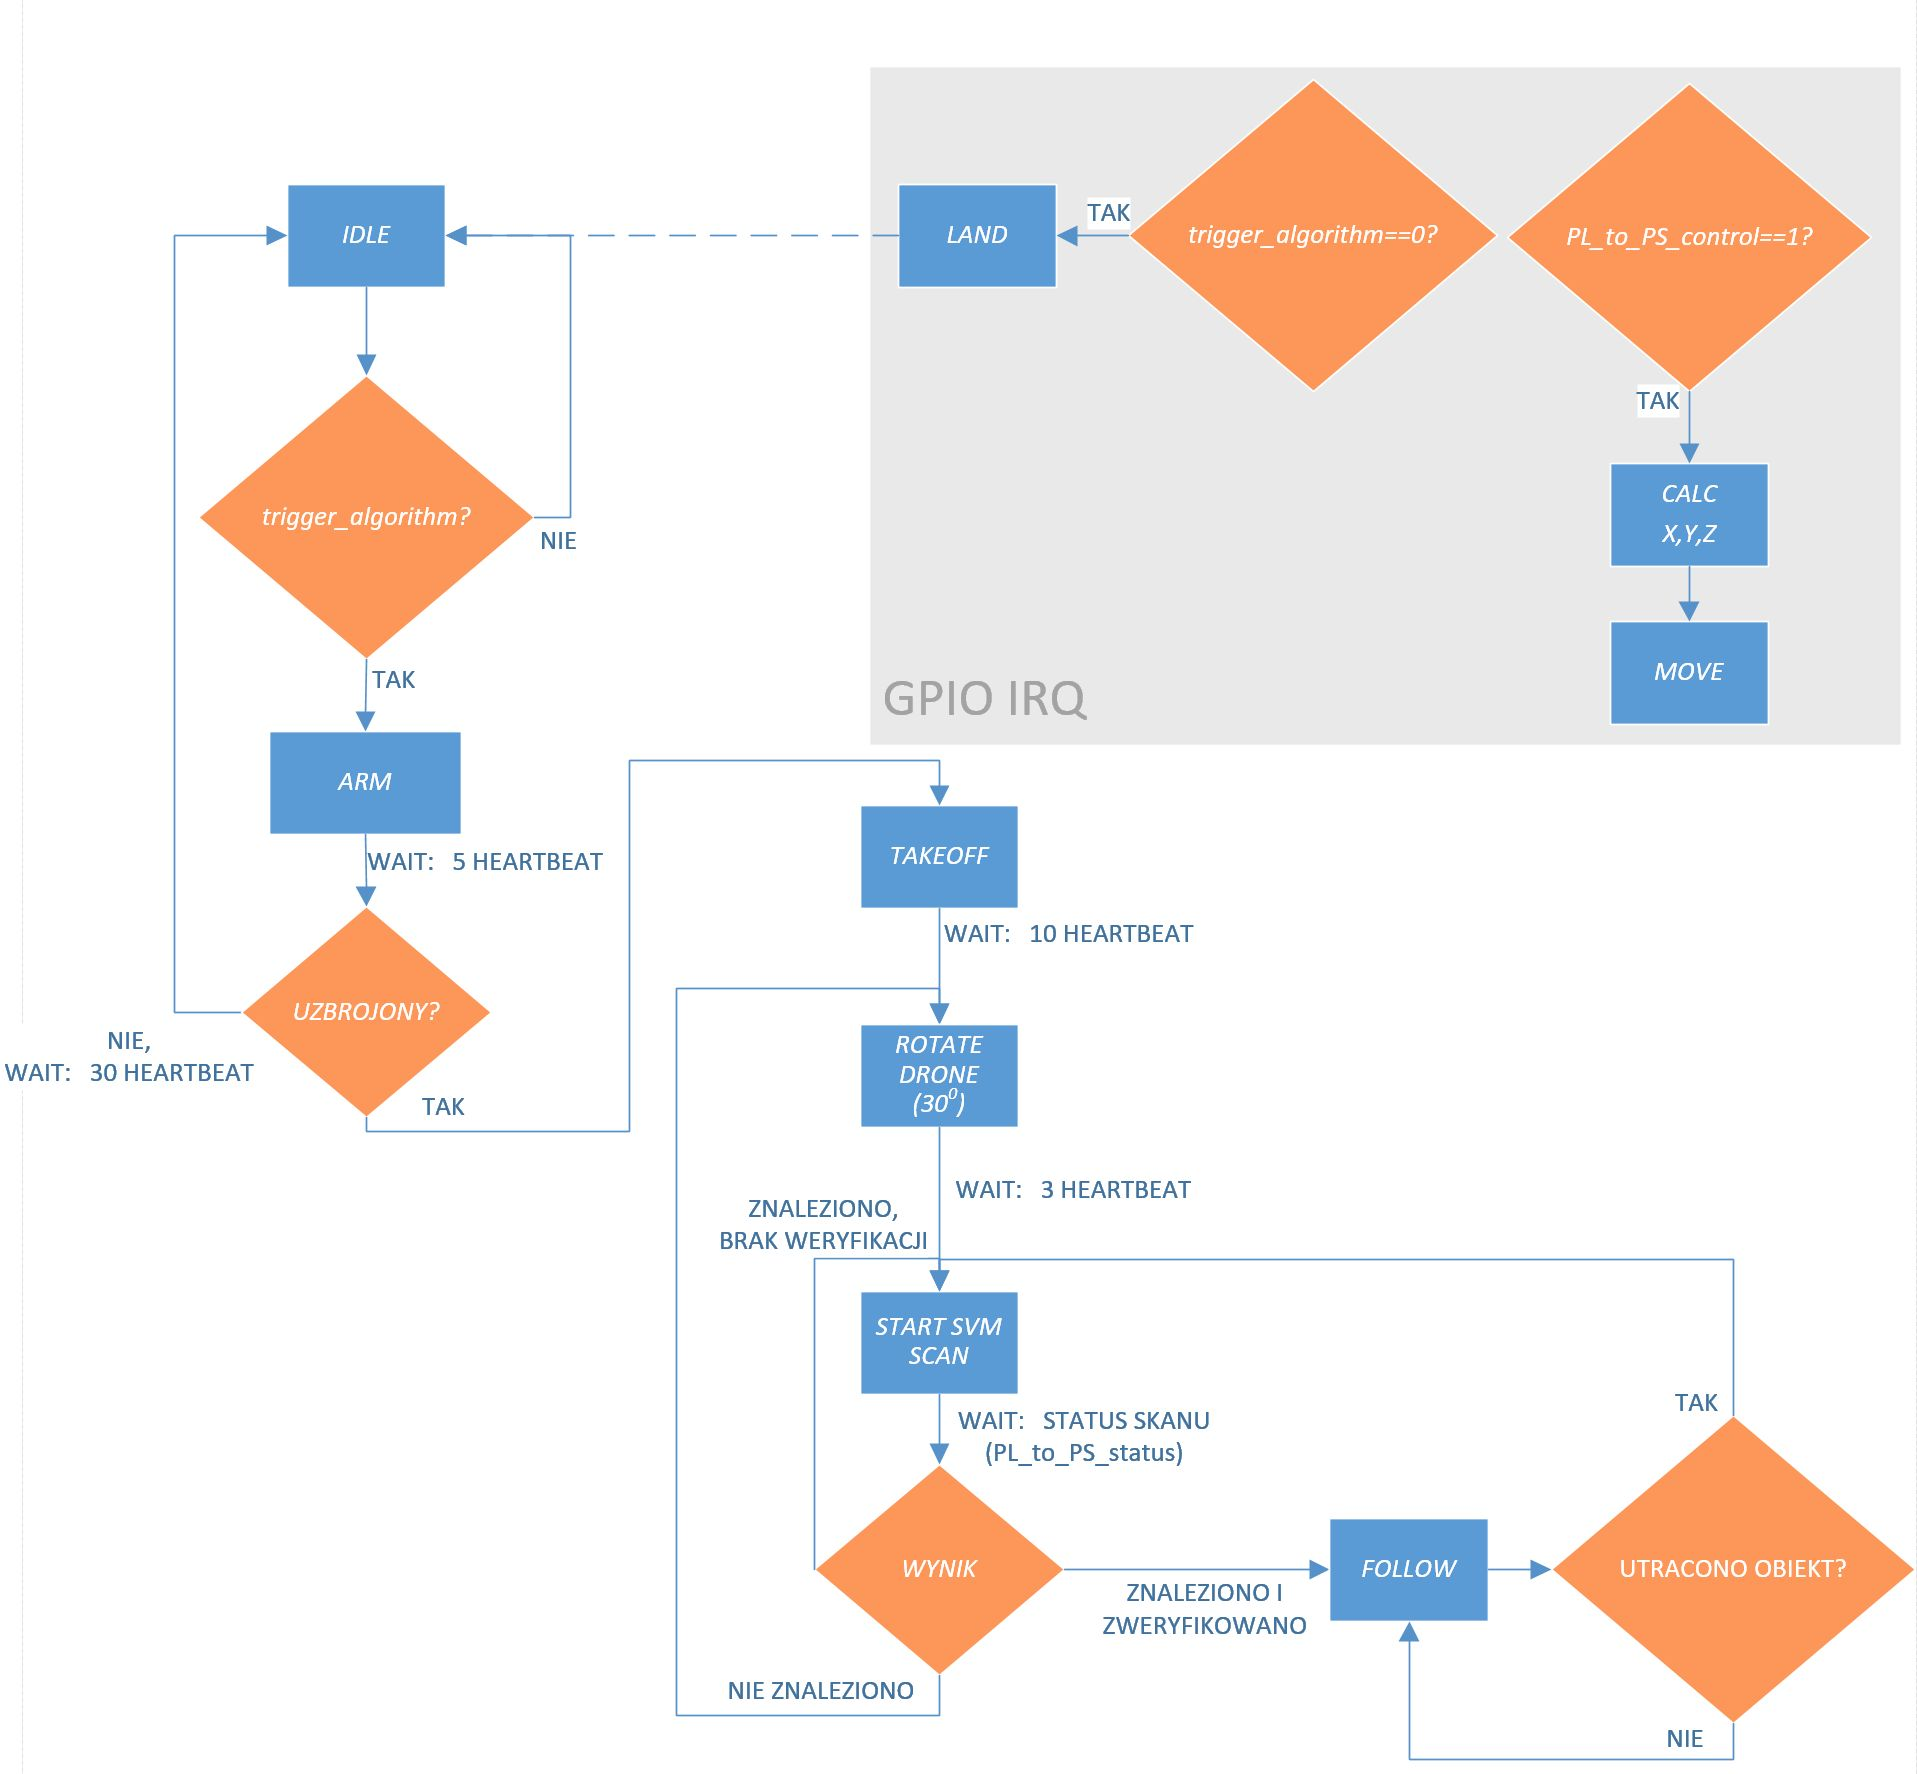
\includegraphics[width=16cm]{5_PS_FSM.jpg}
\caption{Nadrzędny schemat działania systemu}
\label{fig:PL_FSM_sch}
\end{figure}

%TODO Brak omówienia schematu

%TODO a jakieś ograniczenia na ten ruch. min z max z maks zmiana ?
\chapter{Weryfikacja działania systemu wizyjnego}
%TODO bardziej inforamtywny tytuł. %ODP OK

Sprawdzenie poprawności działania obu algorytmów miało przebieg trzyetapowy:
\begin{itemize}
	\item model programowy,
	\item symulacja modelu behawioralnego,
	\item uruchomienie algorytmu z warstwą sterującą na dronie.
\end{itemize}
%TODO a model programowy ? %ODP OK

\section{Testy symulacyjne}

Skomplikowanie procesu implementacji sprzętowej wymagało równolegle przeprowadzanych testów symulacyjnych podczas prac nad każdym z algorytmów śledzących. %TODO usunac pierwszą część zdania, druga przeredagować. %ODP OK
Za referencję do symulacji obrano uprzednio stworzony model programowy w MATLABie, chociażby ze względu na wykorzystanie tych samych obrazów w celu porównania wyników. %TODO raczej za referencję. %ODP OK
Moduł symulacyjny stworzony w środowisku Vivado i języku SystemVerilog nie uwzględniał jedynie części logiki zawartej w \textit{Block Design} -- a więc instancji procesora oraz wejściowego i wyjściowego fragmentu toru wizyjnego. 
Testy procesora nie mają związku z testowanymi algorytmami, a mocno spowalniałyby pracę symulatora. %TODO inaczej to ująć. %ODP OK
Jako zamiennik wejścia informacji wizyjnej, wystarczył zasymulowany komplet sygnałów RGB z informacją o wartości piksela, która została wczytana z pliku tekstowego. 
Plik przechowujący jedną ramkę obrazu, wygenerowano w MATLABie umieszczając każdy kolejny piksel w nowej linii w formacie heksadecymalnym, po dwa znaki na każdą składową R, G i B.

Podstawowej zaletą symulacji jest możliwość podejrzenia propagowanych w układzie sygnałów w oknie wyświetlającym ich czasowy przebieg. %TODO zaletą + to przystosowane też inaczej. %ODP OK
Jednak ze względu na zwiększający się poziom skomplikowania projektu, z czasem postanowiono uprościć porównanie wybranych wyników symulacji z pracą modelu programowego. %TODO "rozrastający się". + niejasne %ODP OK
W kodzie architektury stworzono więc logikę zapisującą do plików określone informacje z pojedynczej iteracji algorytmu. 
By jednak zapis nie był realizowany na każdym zboczu narastającym zegara, potrzebne było określenie sygnałów wyzwalających - -zazwyczaj były to odpowiedniki sygnałów aktywnych powiązanych z określoną informacją. 
Do analizy stworzono w MATLABie dodatkowy skrypt, który parsował stworzone podczas symulacji pliki, uruchamiał pojedynczy przebieg modelu programowego i porównywał wyniki, określając liczbę błędów na danym etapie algorytmu dla całej ramki. 
Niektóre dane, z racji ograniczenia bitowej reprezentacji w architekturze, wymagały zdefiniowania akceptowalnego poziomu tolerancji błędu.


\section{Testy w układzie Zynq} %TODO możę konkretnie w Zynq %ODP OK

Symulacje są zbyt kosztownym czasowo narzędziem, dlatego w pewnym momencie należało przejść na testy na urządzeniu PYNQ. 
Proces budowy projektu sprowadza się do stworzenia konfiguracji sprzętowej w Vivado i skompilowania aplikacji uruchamianej na procesorze ARM. %TODO budowy do zbudowania %ODP OK, masakra.
Docelowo układ SoC może być uruchomiony z poziomu karty SD, jednak ze względu na kwestię praktyczności, pozostano przy połączeniu JTAG. 
Stworzona konfiguracja testowa jest przedstawiona na schemacie \ref{fig:testing_setup}. Zastosowaniem komputera (PC \#1) jest nie tylko zaprogramowanie układu Zynq poprzez interfejs JTAG, ale i diagnostyczna komunikacja z układem, realizowana poprzez UART. %TODO \ref + omówienie schematu %ODP OK
Źródłem obrazu wideo może być dowolne urządzenie z możliwością wysłania sygnału \textit{720p} poprzez kabel HDMI. W tym wypadku jest to kamera, albo inny komputer - służący to odtwarzania wcześniej zapisanych materiałów wideo. Najważniejszym elementem podczas testów jest wyświetlenie obrazu wyjściowego, z nakreślonymi obszarami detekcji.
\begin{figure}[h]
	\centering
	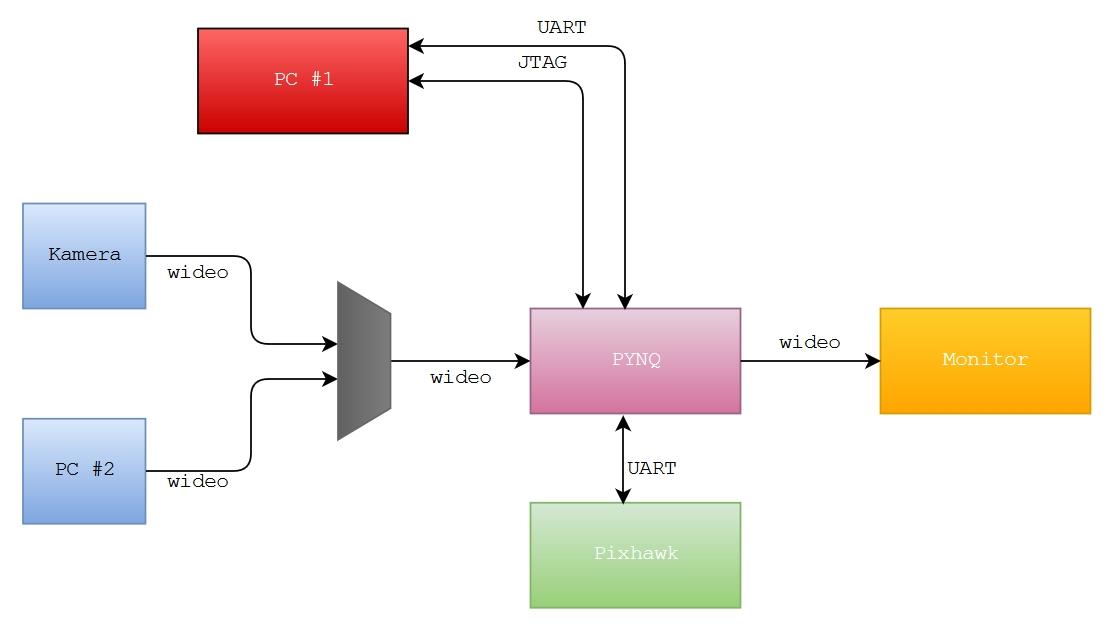
\includegraphics[width=14cm]{6_testing_setup.jpg}
	\caption{Schemat stanowiska testowego}
	\label{fig:testing_setup}
\end{figure}

Test polega na skanowaniu ruchomego obrazu w poszukiwaniu postaci, a następnie śledzeniu znalezionej osoby. Analiza jest rozpoczynana w lewym górnym rogu, po czym sukcesywnie przechodzi w linii poziomej do prawej krawędzi, co jest następnie powtarzane dla niższych pozycji \ref{fig:scan_scheme} %TODO 'ref %ODP OK
Na przykładowych zrzutach z materiału wideo \ref{fig:scan_screenshot} zaprezentowano proces skanowania obrazu. 
Niebieskimi prostokątami oznaczone są aktualne okna detekcji dla poszczególnych skal. 
Zielone okno to obszar śledzenia algorytmem MeanShift, natomiast czerwonym kolorem oznaczono aktualnie najlepsze okno $128 \times 64$ (przeskalowane ponownie do oryginalnej rozdzielczości).

\begin{figure}[h]
	\centering
	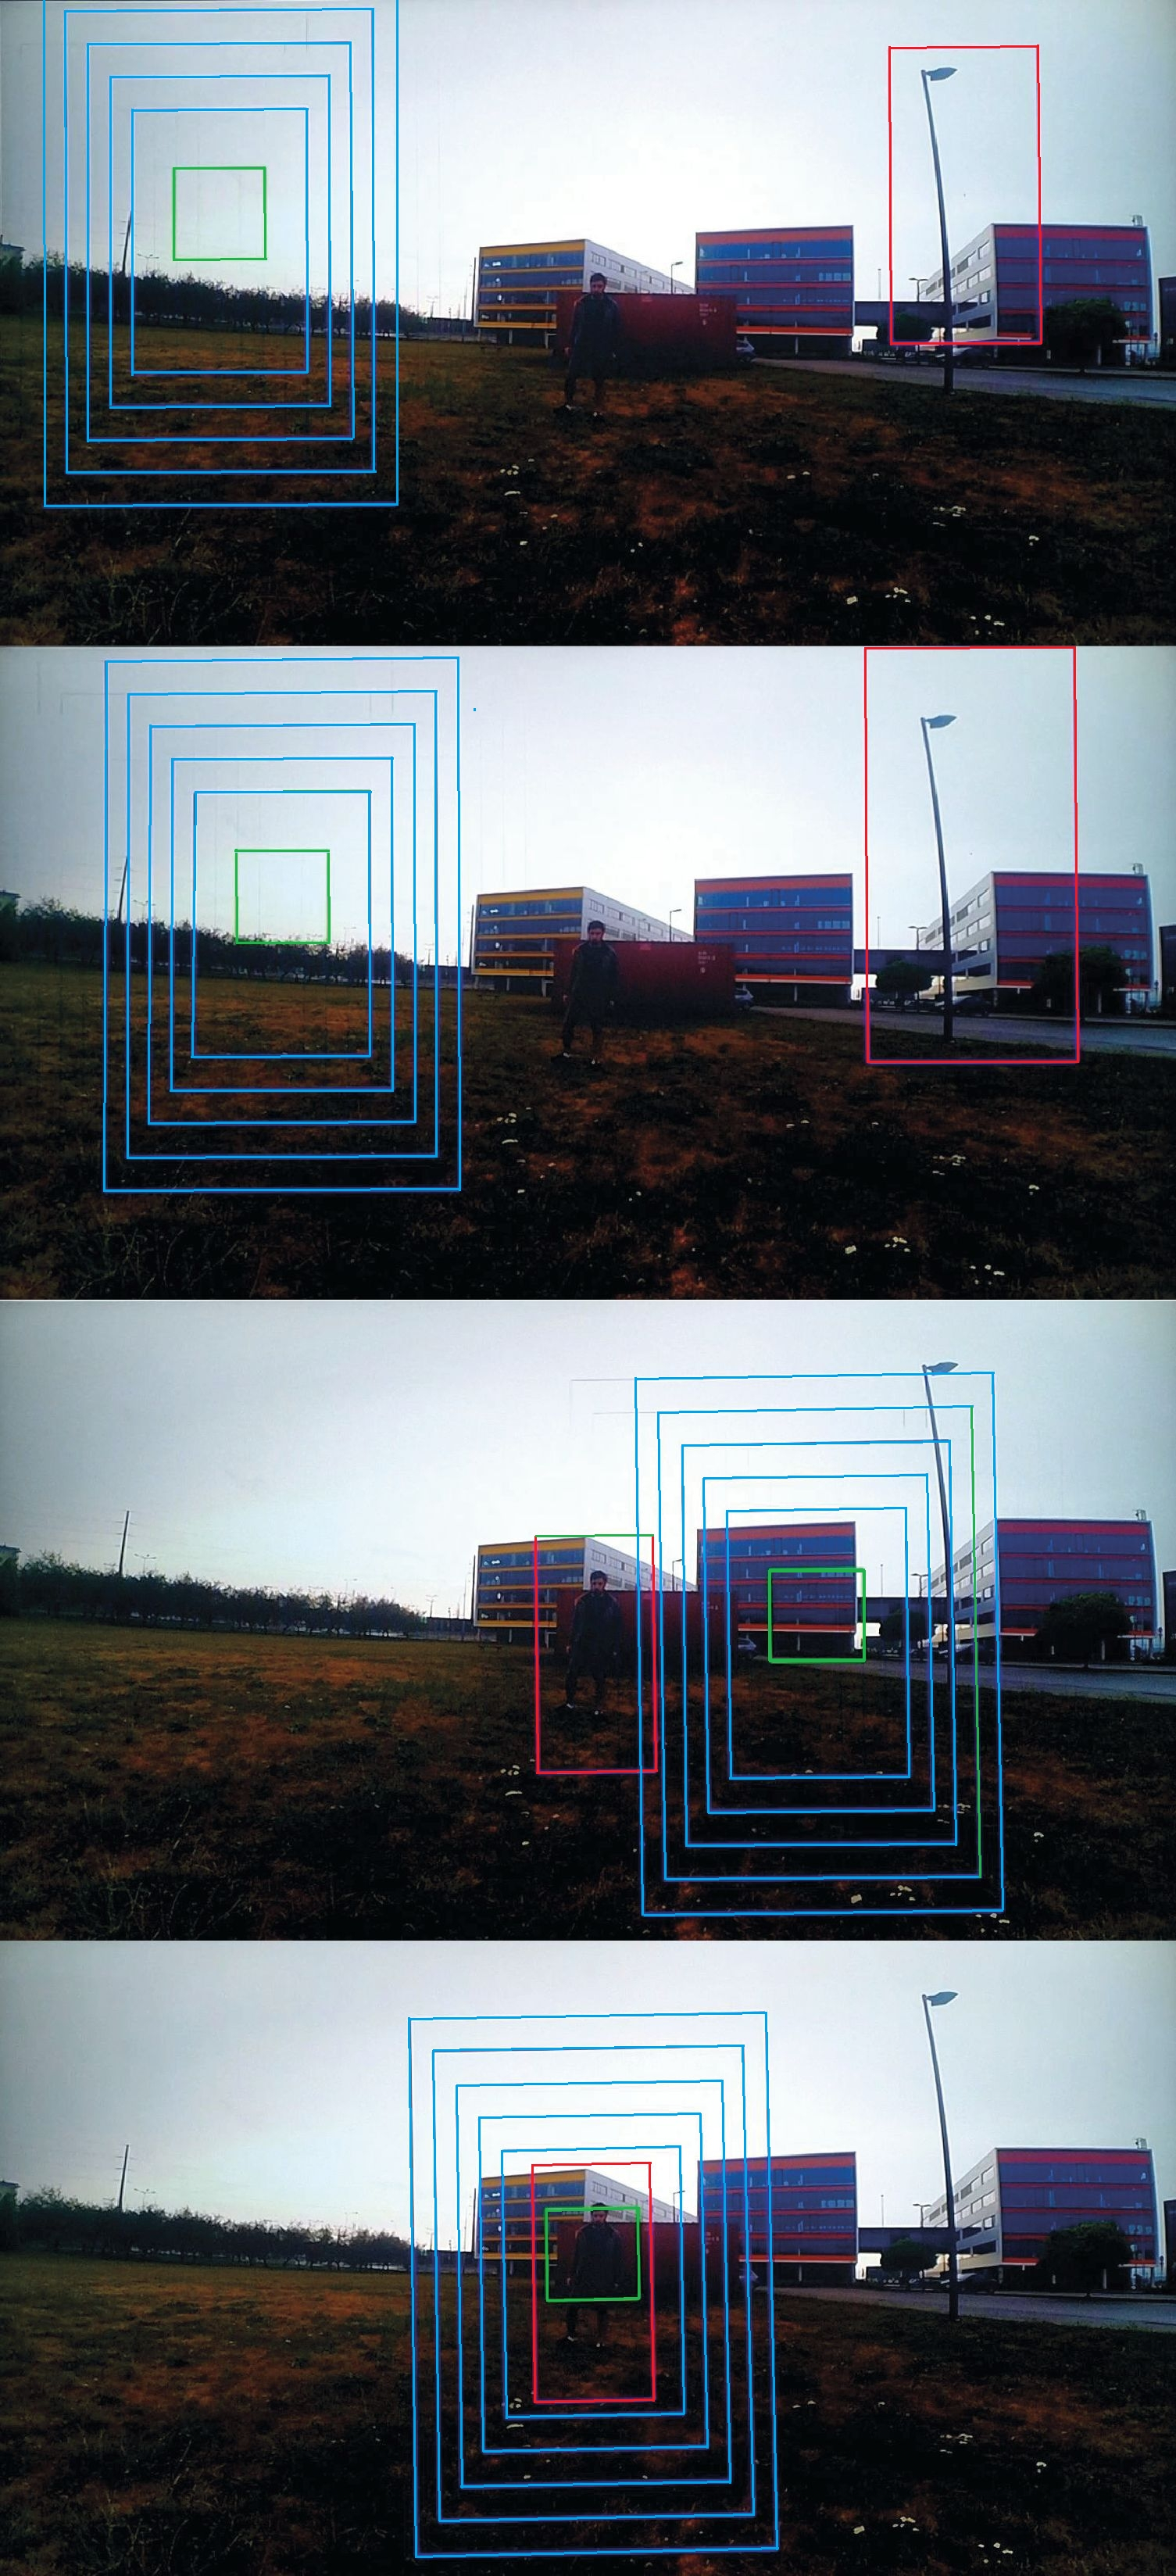
\includegraphics[width=10cm]{6_scan_1.jpg}
	\caption{Proces skanowania} %TODO Ilustracja procesu skanowania + pogrubić ramki w paint :) %ODP OK, prosty schemat wyżej
	\label{fig:scan_screenshot}
\end{figure}

\begin{figure}[h]
	\centering
	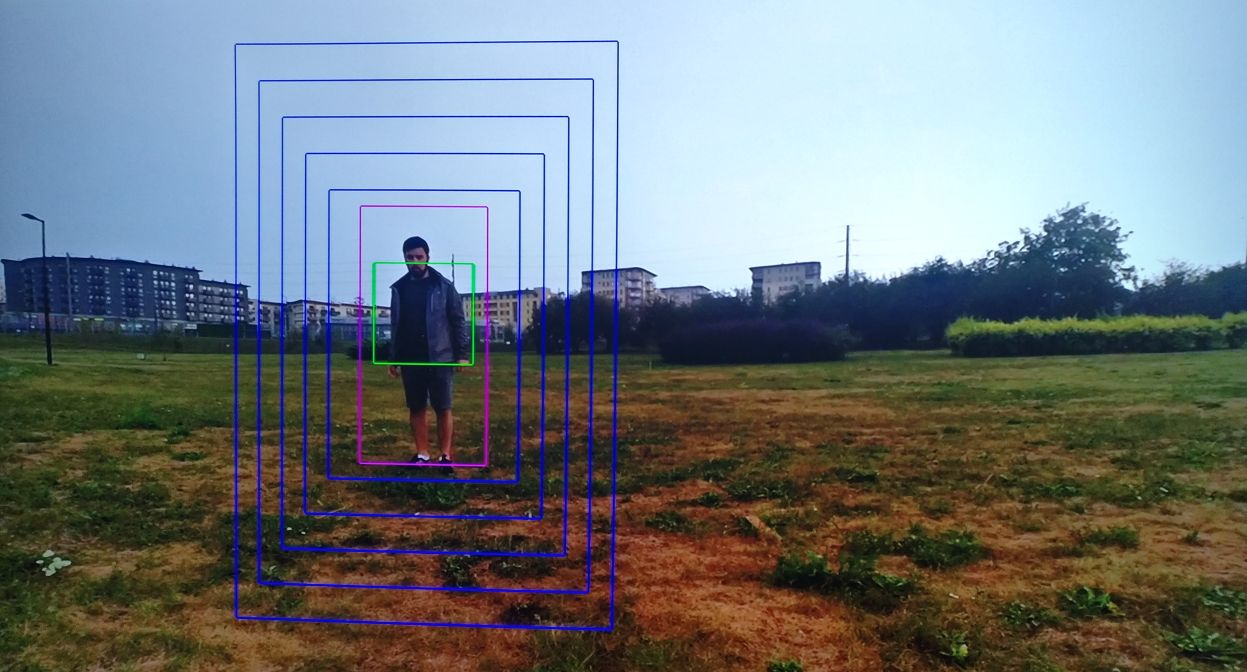
\includegraphics[width=10cm]{6_track_1.jpg}
	\caption{Śledzenie \#1}
	\label{fig:track_1}
\end{figure}

\begin{figure}[h]
	\centering
	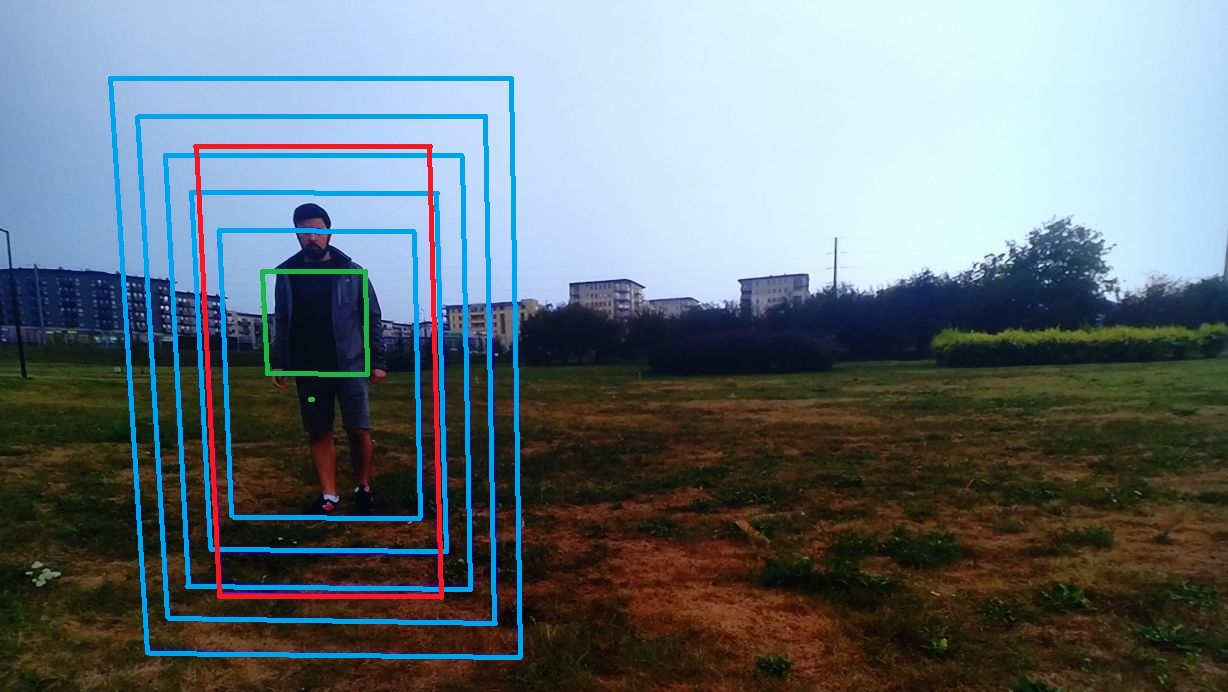
\includegraphics[width=10cm]{6_track_2.jpg}
	\caption{Śledzenie \#2}
	\label{fig:track_1}
\end{figure}

\begin{figure}[h]
	\centering
	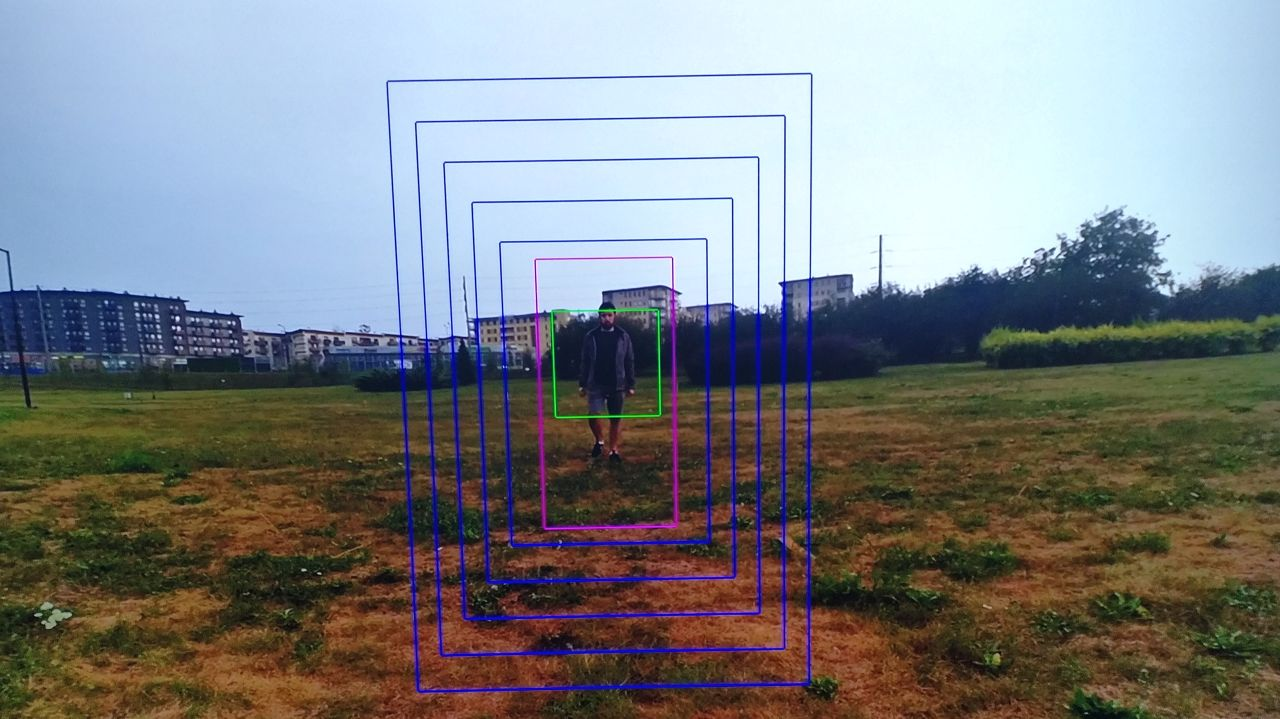
\includegraphics[width=10cm]{6_track_3.jpg}
	\caption{Śledzenie \#3}
	\label{fig:track_1}
\end{figure}

 Przebieg testu powinien być jak najbardziej zbliżony do pracy układu podczas lotu, z tego względu do procedury dodano komunikację UART z autopilotem. Nadzór nad nią jest sprawowany poprzez dodatkowe połączenie szeregowe łączące układ Zynq z komputerem, który wyświetla na terminalu wszystkie istotne komunikaty. Przykładowo, raport \ref{tab:log} przedstawia informacje uzyskane w ciągu pierwszych kilkunastu sekund jednego z testów. Po otrzymaniu sygnału startu (przełącznik na układzie PYNQ lub na aparaturze radiowej) do autopilota wysyłana jest komenda uzbrojenia (ARM) i startu (TAKEOFF), jednak ze względu na obecność drona w budynku niemożliwe jest określenie pozycji poprzez GPS - odesłana wiadomość COMMAND ACK informuje, że wykonanie komendy TAKEOFF (ID: 22) się nie powiodło (status: 4). Podczas testu ten komunikat jest jednak ignorowany, i rozpoczynane jest skanowanie. Po dłuższej chwili otrzymywany jest komunikat o pozytywnym wyniku detekcji, po czym system rozpoczyna zadanie śledzenia. Od tego momentu większość komunikatów dotyczy informacji z PL o odległości śledzonego obiektu od wartości zadanej i skali -- przemnożonej przez 10 z powodu braku funkcji wyświetlającej liczby zmiennoprzecinkowe. Niezależnie od przebiegu pracy systemu wizyjnego mogą pojawiać się wiadomości z autopilota o statusie (INFO) i zmianach parametrów (PARAM VAL). Test jest kończony przez użytkownika poprzez wycofanie sygnału startu - poza zakończeniem pracy algorytmu wysyłana jest wówczas komenda lądowania (LAND).
 
%TODO \ref do tabeli. %ODP OK
%TODO jakieś jednak omówienie. %ODP OK, dodano wyżej


\begin{table}[h]
	\centering\scriptsize 
	
	\begin{tabular}{|p{8cm} |}
		
        \hline
prompt>>ARMING... \\
ARMED! \\
TAKING OFF... \\
Sent TAKEOFF CMD. \\
COMMAND ACK: 22 4 \\
STARTING SEARCH! \\
xDiff: 37        \tab yDiff: 33      \tab| scale: 27 || \\
DATA OK, STARTING FOLLOW! \\
xDiff: 20        \tab yDiff: 20      \tab| scale: 25 || \\
xDiff: 10        \tab yDiff: 20      \tab| scale: 25 || \\
xDiff: 52        \tab yDiff: 38      \tab| scale: 22 || \\
xDiff: 94        \tab yDiff: 8       \tab\tab| scale: 22 || \\
xDiff: 140       \tab yDiff: 12      \tab| scale: 20 || \\
xDiff: 165       \tab yDiff: 30      \tab| scale: 25 || \\
xDiff: 157       \tab yDiff: 22      \tab| scale: 22 || \\
xDiff: 125       \tab yDiff: 40      \tab| scale: 25 || \\
xDiff: 95        \tab yDiff: 35      \tab| scale: 22 || \\
xDiff: 62        \tab yDiff: 26      \tab| scale: 20 || \\
xDiff: 26        \tab yDiff: 28      \tab| scale: 20 || \\
xDiff: 10        \tab yDiff: 28      \tab| scale: 20 || \\
xDiff: -6         \tab\tab yDiff: 28      \tab| scale: 20 || \\
xDiff: -30        \tab yDiff: 36      \tab| scale: 20 || \\
xDiff: -70        \tab yDiff: 28      \tab| scale: 20 || \\
xDiff: -86        \tab yDiff: 20      \tab| scale: 20 || \\
xDiff: -118       \tab yDiff: 28      \tab| scale: 20 || \\
xDiff: -150       \tab yDiff: 12      \tab| scale: 20 || \\
xDiff: -150       \tab yDiff: 12      \tab| scale: 20 || \\
xDiff: -110       \tab yDiff: 20      \tab| scale: 20 || \\
xDiff: -86        \tab yDiff: 20      \tab| scale: 20 || \\
xDiff: -62        \tab yDiff: 28      \tab| scale: 20 || \\
INFO: PreArm: Throttle below Failsafe \\
xDiff: 22        \tab yDiff: 28      \tab| scale: 20 || \\
xDiff: 30        \tab yDiff: 4       \tab\tab| scale: 22 || \\
xDiff: 62        \tab yDiff: 42      \tab| scale: 27 || \\
xDiff: 95        \tab yDiff: 33      \tab| scale: 27 || \\
xDiff: 107       \tab yDiff: 33      \tab| scale: 30 || \\
xDiff: 107       \tab yDiff: 33      \tab| scale: 30 || \\
xDiff: 107       \tab yDiff: 33      \tab| scale: 30 || \\
xDiff: 172       \tab yDiff: 34      \tab| scale: 20 || \\
PARAM VAL: 0 1083785216 769  1898664 \\
PARAM VAL: 0 1091798652 769  1898664 \\
xDiff: 268       \tab yDiff: 14      \tab| scale: 20 || \\
xDiff: 368       \tab yDiff: 14      \tab| scale: 22 || \\
xDiff: 450       \tab yDiff: 20      \tab| scale: 25 || \\
xDiff: 560       \tab yDiff: 15      \tab| scale: 22 || \\
Sent LAND CMD. \\
COMMAND ACK: 21 0 \\    
\hline 	
	\end{tabular}
	\caption{Przykładowa zawartość terminala ze śledzenia na podstawie gotowego materiału wideo}
	\label{tab:log}
\end{table}
\chapter{Podsumowanie i możliwości rozwoju pracy}

W zrealizowanym projekcie przedstawiono sprzętową realizację detekcji i śledzenia osoby w heterogenicznym układzie Zynq SoC, na potrzeby kontroli bezzałogowego statku powietrznego. 
Osiągnięto przetwarzanie obrazu o rozdzielczości $1280\times 720$ dla 60 klatek na sekundę, z prędkością \textit{60Hz} i \textit{30Hz} odpowiednio dla algorytmów MeanShift oraz HoG+SVM.

Na uwagę zasługuje warstwa najwyższa, łącząca pracę obu algorytmów i komunikująca się z autopilotem Pixhawk. 
Wykorzystanie protokołu MAVLink pozwala stworzyć platformę, która jest w stanie wydawać polecenia ruchu bez udziału pilota.

%TODO jeszcze o budowie. Ogólnie nieco obszerniej by to można opisać.

Autor uważa jednak, że bazując na testowanej konfiguracji sprzętowo-programowej można dokonać szeregu usprawnień, podnoszących ogólną niezawodność rozwiązania. %TODO to jednak tu nie pasuje
Jednym z nich jest próba zredukowania liczby fałszywych detekcji (HoG+SVM) poprzez zmianę wielkości bloków lub komórek. %TODO no właśnie, jakoś Pan to testował ? Bo chyba tego tam nie ma.
Innym pomysłem mogłoby być proste zwiększenie liczby analizowanych skal. %TODO liczby ? %ODP OK
Kolejnym usprawnieniem, tym razem dla algorytmu MeanShift, byłoby zlikwidowanie rzadkich sytuacji utraty zbieżności ze śledzonym obszarem -- co skutkuje „wędrowaniem okna”. %TODO wie Pan dlaczego ?
Barierą na drodze większości zmian jest liczba dostępnych zasobów w układzie -- wymagana byłaby zmiana układu na dysponujący zwłaszcza większą liczbą bloków BRAM. 
Istnieją jednak zmiany niewymagające ingerencji w kod. 
Do podstawowych należałby lepszy dobór ustawień programowych kamery w celu poprawy rejestrowanych (wysyłanych kablem) kolorów. Kamery sportowe są wyposażone w wiele usprawnień (tryb nocny, rektyfikacja,itp.), które niekoniecznie muszą poprawiać działanie systemu wizyjnego %TODO to jest niejasne, a ważne %ODP OK
Kolejną mogłaby być lepsza stabilizacja obrazu - ze względu na podpięty do kamery kabel zmienia się jej środek ciężkości, co zaburza pracę gimbala - silnik na jednej z osi obrotu musiał nawet być z tego powodu wyłączony. %TODO szczegóły %ODP OK
Ostatnią, mającą największy wpływ na śledzenie, byłoby poprawienie właściwości lotnych drona. Mowa tu głównie o problemach z płynnością ruchu oraz utrzymywaniem drona w zadanej pozycji - co może mieć związek z ustawieniami akceleratorów lub przetwarzaniem sygnału GPS.%TODO j.w. %ODP OK

Ponadto, zbudowana platforma stanowi ogromny potencjał dla nowych pomysłów związanych z autonomizacją dronów. 
Podstawowym kierunkiem mogłaby być zdolność omijania przeszkód (nadal kosztowna opcja w dronach komercyjnych). Detekcja mogłaby być realizowana przez specjalistyczne czujniki odległościowe, stereowizję lub nawet lidar. %TODO odległościowe, sterowizja, lidar %ODP OK




\appendix
\renewcommand{\thechapter}{\Alph{chapter}}
\chapter{Spis zawartości płyty CD}

Dołączona do pracy płyta CD zawiera następujące pliki i katalogi:
\begin{itemize}
	\item praca.pdf -- plik zawierający tekst pracy magisterskiej w formacie \textit{pdf},
	\item MATLAB -- katalog zawierający pliki modelów programowych, a także pliki wideo służące do testów oraz zestaw treningowy SVM „INRIA Person dataset”,
	\item PYNQ -- katalog zawierający projekt z plikami źródłowymi (PL oraz PS) do zbudowania i uruchomienia na układzie PYNQ,
	\item Praca\_TEX -- katalog zawierający pliki \LaTeX z tekstem pracy magisterskiej oraz wykorzystanymi w niej rysunkami.
\end{itemize}


\printbibliography

\end{document}
